\documentclass[11pt]{article}	% Always compile at least twice.
% Cover Information	
\def\univname{}
\def\coursenum{}
\def\coursename{Abstract Algebra}
\def\professor{Aryaman Maithani}
\def\student{Ishan Kapnadak}
\def\semesteryear{Summer of Science 2021}
\def\imagename{iitb.png}		    % Replace with University Seal
\def\scalesize{0.20}					% Scale Logo Size 

% Style Package (Load After Cover Information)
\usepackage{aryaman}	% Change to match style file
%\setcounter{tocdepth}{1}
%\definecolor{arsenic}{rgb}{0.23, 0.27, 0.29}
\definecolor{arsenic}{rgb}{0.43, 0.5, 0.5}
% -------------------
% Content
% -------------------
\begin{document}


% Cover Page
\coverpage

\newpage
% Last Updated
\thispagestyle{empty}
\vspace*{\fill}
\begin{center}
    \textbf{ABSTRACT}
    
    \medskip
    \begin{minipage}{15cm}
    \begin{center}
        We begin with a brief discussion of Number Theory. Then, we move on to Group Theory, where we cover examples of groups, homomorphisms, quotient groups, isomorphism theorems, group actions, and Sylow's theorems. We then move on to Ring Theory, covering rings, fields, homomorphisms, domains, and polynomial rings. Finally, we cover introductory Galois Theory, discussing algebraic extensions, separable extensions, normal extensions, Galois extensions, and end by stating the Fundamental Theorem of Galois Theory.
    \end{center}
    \end{minipage}
    
\end{center}
\vspace*{\fill}


% Table of Contents
\thispagestyle{empty}
\tableofcontents
% \newpage
\pagestyle{fancy}
\setcounter{section}{-1}
\setcounter{page}{1}

\addcontentsline{toc}{section}{\large{\textbf{\textcolor{arsenic}{Preliminaries}}}}
\section{Preliminaries}

\subsection{Notation}

\begin{enumerate}
    \item $\N = \{ 0, 1, 2, \ldots \}$ is the set of non-negative integers
    \item $\N^+ = \{ 1, 2, 3, \ldots \}$ is the set of positive integers
    \item $\Z = \{ 0, \pm 1, \pm 2, \ldots \}$ is the set of integers
    \item $\Q = \left\{ \frac{m}{n} \mid m,n \in \Z, n \neq 0 \right\}$ is the set of rationals
    \item $\R$ is the set of reals
    \item $\C$ is the set of complex numbers
    \item $\Q^{\times}$, $\Z^{\ast}$, $\R^{\times}$, $\C^{\times}$ will denote the set of non-zero rationals, integers, reals and complex numbers respectively.
\end{enumerate}

\subsection{Relations and Partitions}

\begin{defn}
    A \deff{relation} on $A$ is a subset $R$ of $A \times A$. If $(a,b) \in R$, we say that $a$ is \deff{related to} $b$ by $R$ and write $a \, R \, b$ or $a \sim  b$.
\end{defn}

For example, `equality' (=) is a relation on any set $A$. `Less than' ($<$) is a relation on $\R$ or any of its subsets. Fix a positive integer $n$. Then, `congruence modulo $n$' ($\equiv)$ is a relation on $\Z$, defined by 
\[
    a \equiv b \Mod{n} \iff n \divides a-b.
\]

\begin{defn}
    A relation $\sim$ on $A$ is said to be an \deff{equivalence relation} if it is
    \begin{enumerate}
        \item \deff{reflexive}, i.e, $a \sim a$ for all $a \in A$,
        \item \deff{symmetric}, i.e, $a \sim b$ implies $b \sim a$ for all $a,b \in A$, and
        \item \deff{transitive}, i.e, $a \sim b$ and $b \sim c$ implies $a \sim c$ for all $a,b,c \in A$.
    \end{enumerate}
\end{defn}

It is easy to show that $<$ is transitive but not reflexive or symmetric. $=$ is an equivalence relation on any set whereas $\equiv \Mod{n}$ is an equivalence relation on $\Z$.

\begin{exe} \label{exe:equivalence-Z-Q}
\phantom{hi}
\begin{enumerate}
    \item Show that the relation $\sim$ on $\N \times \N = \left\{ (m,n) \mid m,n \in \N \right\}$ defined by
    \[
        (m,n) \sim (m^{\prime}, n^{\prime}) \iff m + n^{\prime} = m^{\prime} + n
    \]
    is an equivalence relation.
    
    \item Show that the relation $\sim$ on $\Z \times \Z^{\ast} = \left\{ (m,n) \mid m,n \in \Z, n \neq 0 \right\}$ defined by
    \[
        (m,n) \sim (m^{\prime}, n^{\prime}) \iff m \cdot n^{\prime} = m^{\prime} \cdot n
    \]
    is an equivalence relation.
\end{enumerate}
\end{exe}


\begin{rem}[Well-Ordering Property] \label{rem:wop}
     Every non-empty subset of $\N$ has a least element. That is, if $A \subseteq \N$ and $A \neq \emptyset$ then $\exists \, m \in \N$ such that $m \leq a$ for all $a \in A$. WOP is also true for any subset of $\Z$ which is bounded below. WOP also implies the principle of induction.
\end{rem}

\begin{defn}
    If $\sim$ is an equivalence relation on $A$, then for any $a \in A$, the set
    \[
        [a]_{\sim} \vcentcolon= \{ b \in A \mid b \sim a \}
    \]
    is called the \deff{equivalence class} of $a$ with respect to $\sim$. Elements of the equivalence class of $a$ are said to be \deff{equivalent} to $a$. If $C$ is an equivalence class, then any element of $C$ is called a \deff{representative} of class $C$. We will denote the equivalence class of $a$ as $[a]$ when the relation $\sim$ is clear from context.
\end{defn}



\begin{ex}
    Fix some $n \in \N_+$ and consider the equivalence relation $\equiv \Mod{n}$. We have a total of $n$ equivalence classes, defined by
\begin{align*}
    [0] &= \left\{ kn \mid k \in \Z \right\} \\
    [1] &= \left\{ kn + 1 \mid k \in \Z \right\} \\
    \vdots \, &= \quad \vdots \\
    [n-1] &= \left\{ kn + n-1 \mid k \in \Z \right\}
\end{align*}

These are called the \emph{residue classes$\Mod{n}$}. We sometimes also denote the residue classes as $\overline{0}, \overline{1}, \ldots, \overline{n-1}$. We denote the set of residue classes of $n$ as $\Z_n$, defined as
\[
    \Z_n \vcentcolon= \left\{ \overline{0}, \overline{1}, \ldots, \overline{n-1} \right\}.
\]
For $\overline{a}, \overline{b} \in \Z_n$, we further define addition and multiplication as follows
\[
    \overline{a} + \overline{b} = \overline{a + b} \text{ and } \overline{a} \cdot \overline{b} = \overline{a \cdot b}.
\]
One may verify that these operations are indeed well-defined.
\end{ex}
\begin{exe}
The following exercise builds on \Cref{exe:equivalence-Z-Q}.
\begin{enumerate}
    \item Show that the equivalence classes of the relation $\sim$ on $\N \times \N = \left\{ (m,n) \mid m,n \in \N \right\}$ defined by
    \[
        (m,n) \sim (m^{\prime}, n^{\prime}) \iff m + n^{\prime} = m^{\prime} + n
    \]
    are in one-to-one correspondence with the set of integers. (We may define the set $\Z$ formally, using $\N$, as equivalence classes of this relation).
    
    \item Show that the equivalence classes of the relation $\sim$ on $\Z \times \Z^{\ast} = \left\{ (m,n) \mid m,n \in \Z, n \neq 0 \right\}$ defined by
    \[
        (m,n) \sim (m^{\prime}, n^{\prime}) \iff m \cdot n^{\prime} = m^{\prime} \cdot n
    \]
    are in one-to-one correspondence with the set of rationals. (We may define the set $\Q$ formally, using $\Z$, as equivalence classes of this relation).
\end{enumerate}
\end{exe}

\begin{defn} 
    A \deff{partition} of $A$ is a collection $\left\{ A_i \mid i \in I \right\}$ of non-empty subsets of $A$ ($I$ is some indexing set) such that
    \begin{enumerate}
        \item $A = \bigcup_{i \in I} A_i$.
        \item $A_i \cap A_j = \emptyset$ for all $i,j \in I$ with $i \neq j$.
    \end{enumerate}
\end{defn}

The ideas of an equivalence relation and partitions are closely related, as we show now.

\begin{prop} \label{prop:equivalence-partition}
    Let $A$ be a non-empty set.
    \begin{enumerate}
        \item If $\sim$ defines an equivalence relation on $A$ then the set of equivalence classes of $\sim$ form a partition of $A$.
        \item If $\left\{ A_i \mid i \in I \right\}$ is a partition of $A$ then there exists an equivalence relation $\sim$ on $A$ whose equivalence classes are precisely the sets $A_i, i \in I$.
    \end{enumerate}
\end{prop}

\subsection{Number Theory}

\begin{defn}
    Given $a,b \in \Z$, we say that $b$ \deff{divides} $a$ and write $b \divides a$ if $a = bc$ for some $c \in \Z$. In this case, $a$ is said to be a \deff{multiple} of $b$, or $a$ is said to be \deff{divisible} by $b$.
\end{defn}

\begin{enumerate}
    \item Divisibility is a relation on $\Z$, which is reflexive and transitive but not symmetric. In fact, $a \divides b$ and $b \divides a \iff b = \pm a$. This follows since $b \divides a \implies \abs{b} \leq \abs{a}$ (assuming $a \neq 0$).
    \item If $b \divides a_1$ and $b \divides a_2$ then $b \divides (a_1 + a_2)$ and $b \divides ka_1$ for all $k \in \Z$. Thus, $b \divides (k_1a_1 + k_2a_2)$ for all $k_1,k_2 \in \Z$.
\end{enumerate}

\begin{prop}[Division Algorithm] \label{prop:div_algo}
    Given $a,b \in \Z$ with $b \neq 0$, there exist unique $q,r \in \Z$ such that $a = bq + r \text{ and } 0 \leq r < \abs{b}$.
\end{prop}

\begin{proof}
    We first prove existence. Let $a,b \in \Z$ with $b \neq 0$. Without loss of generality, we may assume $b > 0$ (if $b < 0$, we do the following considering $-b$ and replace $q$ by $-q$). Consider
    \[
        S \vcentcolon= \{ a - bx \mid x \in \Z \text{ such that } a - bx \geq 0 \}.
    \]
    Then, $S$ is a non-empty subset of $\N$ (we may take $x = -\abs{a}$). Hence, by the \nameref{rem:wop}, there exists a minimal element in $S$. Call this $r$. Since $r \in S$, $r = a - bq$ for some $q \in \Z$ and $r \geq 0$. We now only have to show that $r < b$. Suppose $r \geq b$, then $r - b = a - b(q+1) \geq 0$ and thus $r-b \in S$. This contradicts the minimality of $r$. This proves the existence of $q,r$ satisfying the given properties.
    
    \medskip
    
    Suppose there are $q,r,q^{\prime}, r^{\prime} \in \Z$ satisfying the given conditions. We have $r - r^{\prime} = b(q{\prime} - q)$. If $r \neq r^{\prime}$, we obtain $\abs{b} < \abs{r - r^{\prime}}$ which is a contradiction since $0 \leq r, r^{\prime} < b$. Thus, we get $r = r^{\prime}$. Since $b \neq 0$, we also get $q = q^{\prime}$. Hence, $q$ and $r$ are unique.
\end{proof}

\begin{cor} \label{cor:additive_subgroup_nZ}
    Suppose $H$ is a subset of $\Z$ that is non-empty and closed under inverses and addition. Then, $H = n\Z$ for a unique $n \in \N$ where
    \[
        n\Z \vcentcolon= \left\{ nm \mid m \in \Z \right\}
    \]
    $H$ is called a \emph{subgroup} of the additive group $\Z$, as we shall see later.
\end{cor}
\begin{proof}
    Let $H$ be a subset of $\Z$ satisfying the given conditions. If $H = \{0\}$ then $H = n\Z$ with $n=0$. If $H \neq \{0\}$, then $H \cap \N^+$ is non-empty. Suppose $n$ is the least element in $H \cap \N^+$ (such an $n$ exists by the \nameref{rem:wop}). Then, $n\Z \subseteq H$ since $H$ is closed under addition. Further, if $m \in H$ then, by the \nameref{prop:div_algo}, there exist $q,r \in \Z$ such that $m = nq + r$ with $0 \leq r < n$. But $r = m - nq \in H$ since $m \in H$ and $n \in H$. If $r > 0$ then $r \in H \cap \N^+$ and the minimality of $n$ is contradicted. Hence, $r = 0$ and $m = nq$. Thus, $H \subseteq n\Z$, giving us $H = n\Z$.
\end{proof}

\begin{defn}
    Given $a,b \in \Z$, not both zero, a \deff{greatest common divisor} or \deff{$\gcd$} of $a$ and $b$ is a positive integer $d$ such that
    \begin{enumerate}
        \item $d$ is a common divisor of $a$ and $b$, i.e, $d \divides a$ and $d \divides b$, and
        \item if $e$ is a common divisor of $a$ and $b$, i.e, $e \divides a$ and $e \divides b$, then $e \divides d$.
    \end{enumerate}
    In the case $a = b =0$, we define the $\gcd$ of $a$ and $b$ to be $0$. We usually denote the $\gcd$ of $a$ and $b$ as $\gcd(a,b)$.
\end{defn}
We leave it as an exercise to the reader to come up with a similar definition for the least common multiple ($\lcm$). We denote the $\lcm$ of $a$ and $b$ as $\lcm(a,b)$.

\begin{prop}[Bézout's Lemma] \label{prop:bezout}
    Given any $a,b \in \Z$, the $\gcd$ of $a$ and $b$ exists and is unique. Moreover, it can be expressed as a combination $ma + nb$ for some $m,n \in \Z$.
\end{prop}
    
\begin{proof}
    For $a=b=0$, the proof is trivial. We hence assume that at least one of $a$ and $b$ is non-zero. Consider 
    \[
        H = \{ ma + nb \mid m,n \in \Z \}.
    \]
    $H$ is a non-empty subset of $\Z$ that is closed under inverses and addition. Hence, by \Cref{cor:additive_subgroup_nZ}, there exists a unique $d \in\N^+$ such that $H = d\Z$. We leave it as an exercise to show that $d$ is indeed the $\gcd$. 
\end{proof}

\begin{prop} \label{prop:a|c}
    \item Let $a,b,c \in \Z$. If $a \divides bc$ and $\gcd(a,b) = 1$ ($a$ and $b$ are coprime), then $a \divides c$.
\end{prop}
\begin{proof}
    \nameref{prop:bezout} tells us that $ma + nb = 1$ for some $m,n \in \Z$. Multiplying throughout by $c$, we get 
    \[
        mac + nbc = c.
    \]
    Since $a \divides ac$ and $a \divides bc$, we must have $a \divides c$.
\end{proof}
\begin{defn}[Prime Number]
    An integer $p$ is said to be a \deff{prime number} if it is greater than $1$ and the only positive integers that divide $p$ are $1$ and $p$.
\end{defn}
\begin{cor}[Euclid's Lemma] \label{cor:euclid_lemma}
    If $p$ is a prime number, and $p \divides bc$ for some $b,c \in \Z$, then $p\divides b$ or $p\divides c$.
\end{cor}
\begin{proof}
    Suppose $p$ is prime and $p \divides bc$ for some $\Z$. If $p \divides b$, we are done. If $p \notdivides b$, then $\gcd(p,b) = 1$. By \Cref{prop:a|c}, $p \divides c$.
\end{proof}

\begin{prop} \label{prop:infinite_primes}
    There are infinitely many primes.
\end{prop}
\begin{proof}[Euclid's Proof]
    If there were only finitely many primes $p_1, \ldots, p_k$, then consider $n = p_1 \cdots p_k + 1$. If $p$ is a prime that divides $n$ then $p \neq p_i$ for all $i \in \{1, \ldots, k\}$ (since $n \equiv 1\Mod{p_i}$ for all $i$), which is a contradiction since $p_1, \ldots, p_k$ are assumed to be the only primes.
\end{proof}

\begin{prop} \label{prop:mult-inverse-mod-p}
    If $b \in \Z$ and $p$ is a prime number such that $p \notdivides b$, then there exists $b^{\prime} \in \Z$ such that $bb^{\prime} \equiv 1 \Mod{p}$. Moreover, $b^{\prime}$ can be chosen such that $1 \leq b^{\prime} < p$ and $b^{\prime}$ is unique.
\end{prop}
\begin{proof}
    Since $\gcd(b,p) = 1$, we have $pu + bv = 1$ for some $u,v \in \Z$ (\nameref{prop:bezout}). Thus, $b^{\prime} = v$ satisfies $bb^{\prime} \equiv 1 \Mod{p}$. The uniqueness of $b^{\prime}$ satisfying $bb^{\prime} \equiv 1 \Mod{p}$ and $1 \leq b^{\prime} < p$ follows by replacing any $v \in \Z$ satisfying $bv \equiv 1 \Mod{p}$ by the unique element $b^{\prime}$ in the residue class of $v \Mod{p}$ such that $0 \leq b^{\prime} < p$. Moreover, $b^{\prime} = 0 \implies 0 \equiv 1 \Mod{p}$ which is a contradiction. Hence, $1 \leq b^{\prime} < p$.
\end{proof}

\begin{theorem}[Fundamental Theorem of Arithmetic] \label{thm:FTAr}
    Every positive integer $n$ can be written as a product of primes. That is,
    \[
        n = p_1 \cdots p_k
    \]
    for some primes $p_1, \ldots, p_k$ (not necessarily distinct). Moreover, this factorisation is unique up to rearrangement of terms. That is, if
    \[
        n = q_1 \cdots q_l
    \]
    where $q_1, \ldots, q_l$ are primes then $k=l$ and $q_i = p_{\sigma(i)}$ for all $i \in \{1, \ldots, k\}$ for some permutation $\sigma$ of $\{1, \ldots, k\}$.
\end{theorem}
\begin{proof}
    We first prove the existence by induction. If $n=1$, the hypothesis holds with $k = 0$ since the empty product is $1$, by convention. Suppose $n > 1$ and the hypothesis holds for all positive integers strictly less than $n$. If $n$ is prime, the hypothesis clearly holds with $k=1$. If $n$ is not prime, then $n = n_1 n_2$ for some $n_1, n_2 \in \N^+$ with $n_1 < n$ and $n_2 < n$. By the induction hypothesis, both $n_1$ and $n_2$ are finite products of primes and hence, so is $n$. Thus, existence is proved by induction.
    
    Next, we prove uniqueness. Suppose $n \in \N^+$ is written as
    \[
        n = p_1 \cdots p_k
    \]
    and also
    \[
        n = q_1 \cdots q_l
    \]
    where $p_1, \ldots, p_k, q_1, \ldots, q_l$ are primes. We can induct on $k$. If $k = 0$, then $n = 1$ and hence $l = 0$. Hence, $k = l$ and $p_i$'s are a permutation of $q_i$'s (vacuously). Suppose that $k > 1$ and the result holds for $k-1$. Then,
    \[
        p_1 \divides n = q_1 \cdots q_l.
    \]
    Hence, by an obvious extension of \nameref{cor:euclid_lemma}, $p_1 \divides q_j$ for some $j$ since $q_j$ is a prime and $p_1 > 1$, we must have $p_1 = q_j$. Thus,
    \[
        p_2 \cdots p_k = q_1 \cdots q_{j-1} \cdot q_{j+1} \cdots q_l.
    \]
    By induction hypothesis, $k-1 = l-1$, giving us $k=l$, and $p_2, \ldots, p_k$ are a permutation of $q_1, \ldots, q_{j-1}, q_{j+1}, \ldots q_l$. Since we showed $p_1 = q_j$, it follows that $p_1, \ldots, p_k$ is a permutation of $q_1, \ldots, q_l$. Thus, uniqueness is also proved by induction.
\end{proof}
Following is another version of the above theorem.
\begin{theorem}[Fundamental Theorem of Arithmetic - Version 2]  \label{thm:FTAr2}
    Every non-zero integer $n$ can be written as
    \[
        n = \epsilon \cdot p_1^{e_1} \cdots p_h^{e_h}
    \]
    where $\epsilon \in \{1,-1\}$, $p_1, \ldots, p_h$ are distinct primes and $e_1, \ldots, e_h$ are positive integers and $h \geq 0$. Moreover, $p_i$ and $e_i$ are uniquely determined by $n$.
\end{theorem}
This allows us to associate with every prime an `exponent' or `valuation' on the set of non-zero integers. Let $p$ be a prime. We define $\nu_p \colon \Z^{\ast} \to \N$ as follows
\[
    \nu_p(n) = \begin{cases}
        e_i & \text{ if } p = p_i \text{ for some $1 \leq i \leq h$ in the prime decomposition of $n$,}\\
        0 & \text{otherwise.}
    \end{cases}
\]
With this notation, we can write
\[
    n = \epsilon \cdot \prod_{p} p^{\nu_p(n)}
\]
where the product is over all primes. This product is well defined since $\nu_p(n) = 0$ for all but finitely many primes.

\begin{prop} \label{prop:gcd-lcm-prime-factorisation}
    If $m,n \in \Z^{\ast}$, then 
    \[
        \gcd(m,n) = \prod_{p} p^{\min\{\nu_p(m), \nu_p(n)\}}
    \]
    \[
        \lcm(m,n) = \prod_{p} p^{\max\{\nu_p(m), \nu_p(n)\}}
    \]
\end{prop}
\begin{cor} \label{cor:prod-gcd-times-lcm}
    If $m,n \in \Z^{\ast}$ then $\, \abs{m \cdot n} = \gcd(m,n) \cdot \lcm(m,n)$.
\end{cor}
We can extend the function $\nu_p$ to non-zero rationals $(\Q^{\times})$ by defining
\[
    \nu_p\left( \frac{m}{n} \right) \vcentcolon= \nu_p(m) - \nu_p(n) \text{ for } m,n \in \Z^{\ast}
\]
We leave it as an exercise to show that the above is indeed well-defined. This allows us to write every non-zero rational number as a product of primes. Suppose $r \in \Q^{\times}$, then we have
\[
    r = \epsilon \cdot \prod_{p} p^{\nu_p(r)}
\]
where $\epsilon \in \{1,-1\}$ and the product is over all primes. This product is well-defined since $\nu_p(r) = 0$ for all but finitely many primes.

\underline{Note:} By convention, we often define $\nu_p(0) = \infty$. With this, the following is true. 
\begin{prop}  \label{prop:p-val-properties}
    Let $\nu_p \colon \Q \to \Z \cup \{\infty\}$ as defined above for some prime $p$. Then,
    \begin{enumerate}
        \item $\nu_p$ is surjective,
        \item $\nu_p(r) = \infty \iff r = 0$,
        \item $\nu_p(rs) = \nu_p(r) + \nu_p(s)$ for all $r,s \in \Q$, and
        \item $\nu_p(r + s) \geq \min\{\nu_p(r), \nu_p(s)\}$ for all $r,s \in \Q$.
    \end{enumerate}
\end{prop}
\begin{proof}
    Left as an exercise.
\end{proof}

\begin{rem}
    The function $\nu_p \colon \Q \to \Z \cup \{\infty\}$ is called the \emph{$p$-adic valuation of $\Q$}. One can use it to define a norm and a metric on $\Q$, as follows:
\[
    \abs{x}_p \vcentcolon= 2^{-\nu_p(x)} \text{ for all } x \in \Q.
\]
with the convention $2^{-\infty} \vcentcolon= 0$. One can see that
\begin{enumerate}
    \item $\abs{x}_p \geq 0$ and $\abs{x}_p = 0 \iff x =0$.
    \item $\abs{xy}_p = \abs{x}_p \abs{y}_p$.
    \item $\abs{x+y}_p \leq \max\left\{ \abs{x}_p, \abs{y}_p \right\} \leq \abs{x}_p + \abs{y}_p$.
\end{enumerate}
Thus, $\abs{\cdot}_p \colon \Q \to \R$ defines a norm on $\Q$. Further, $d_p \colon \Q \times \Q \to \R$ defined by
\[
    d_p(x,y) \vcentcolon= \abs{x-y}_p \text{ for } x,y \in \Q
\]
defines a metric on $\Q$. Once can consider the completion of $\Q$ with respect to $d_p$ and this gives rise to a set denoted by $\Q_p$ called the field of $p$-adic numbers.\footnotemark\ We will not spend much time on $p$-adic numbers in this document.
\end{rem}
\footnotetext{Within the $p$-adic numbers, we also have the $p$-adic integers, denoted by $\Z_p$. Note this is \textbf{not} the set of residue classes modulo $p$. Since we will not deal with $p$-adic integers in this document, we continue to use the notation $\Z_n$ for the set of residue classes modulo $n$. Another common notation for the same is $\Z/n\Z$.} 

\begin{defn}
    Given $n \in \N^+$, we define $\varphi(n)$ to be the number of integers $a \in \N^+$ with $1 \leq a \leq n$ and $\gcd(a,n) = 1$. $\varphi$ is called \deff{Euler's totient function}.
\end{defn}

We can obtain an explicit formula for $\varphi(n)$ using a very basic counting principle - called the inclusion-exclusion principle.
\begin{theorem}[Principle of Inclusion and Exclusion] \label{thm:inc-exc}
    If $A_1, \ldots, A_r$ are finite sets, then
    \[
        \abs{A_1 \cup \cdots \cup A_r} = \sum_i \abs{A_i} - \sum_{i<j} \abs{A_i \cap A_j} + \sum_{i < j < k} \abs{A_i \cap A_j \cap A_k} - \cdots + (-1)^{r-1} \abs{A_1 \cap \cdots \cap A_r}.
    \]
\end{theorem}
\begin{proof}
    The proof is trivial using induction on $r$.
\end{proof}
For $n \in \N^+$, suppose $p_1, \ldots, p_r$ be the distinct primes that divide $n$. We have
\begin{align*}
    n - \varphi(n) &= \abs{\left\{ a \in \N^+ \mid 1 \leq a \leq n \text{ and } \gcd(a,n) \neq 1 \right\}} \\
    &= \abs{\bigcup_{i=1}^r A_{p_i}}
\end{align*}
where for any $m \in \N^+$ with $m \divides n$, $A_m \vcentcolon= \left\{ a \in \N^+ \mid 1 \leq a \leq n \text{ and } m \divides a \right\}$. Observe that $\abs{A_m} = n/m$. By the \nameref{thm:inc-exc},
\begin{align*}
    n- \varphi(n) &= \sum_i \, \abs{A_{p_i}} - \sum_{i<j} \, \abs{A_{p_i} \cap A_{p_j}} + \sum_{i < j < k} \abs{A_{p_i} \cap A_{p_j} \cap A_{p_k}} - \cdots + (-1)^{r-1} \abs{A_{p_1} \cap \cdots \cap A_{p_r}} \\
    &= \sum_i \, \abs{A_{p_i}} - \sum_{i<j} \, \abs{A_{p_ip_j}} + \sum_{i < j < k} \abs{A_{p_ip_jp_k}} - \cdots + (-1)^{r-1} \abs{A_{p_1 \cdots p_r}} \\
    &= \sum_{i} \, \frac{n}{p_i} - \sum_{i < j} \, \frac{n}{p_ip_j} + \sum_{i < j < k} \, \frac{n}{p_ip_jp_k} - \cdots + (-1)^{r-1} \frac{n}{p_1\cdots p_r}
\end{align*}
\begin{align*}
    \therefore \, \varphi(n) &= n - \sum_{i} \, \frac{n}{p_i} + \sum_{i < j} \, \frac{n}{p_ip_j} - \sum_{i < j < k} \, \frac{n}{p_ip_jp_k} + \cdots + (-1)^{r} \frac{n}{p_1\cdots p_r} \\
    &= n \left( 1 - \sum_{i} \, \frac{1}{p_i} + \sum_{i < j} \, \frac{1}{p_ip_j} - \sum_{i < j < k} \, \frac{1}{p_ip_jp_k} + \cdots + (-1)^{r} \frac{1}{p_1\cdots p_r} \right)
\end{align*}
We can express the above term as a product of $r$ factors. This gives us the famous \emph{Euler's Product Formula}:
\[
    \boxed{\varphi(n) = n \cdot \prod_{p \divides n} \left( 1 - \frac{1}{p} \right)}
\]
\begin{cor}[Multiplicativity of $\varphi$] \label{cor:phi-multiplicity}
    For $m,n \in \N^+$, $\varphi(mn) = \varphi(m)\cdot \varphi(n)$ iff $\gcd(m,n) = 1$.
\end{cor}
If $n = p_1^{e_1} \cdots p_h^{e_h}$ where $p_1, \ldots, p_k$ are distinct primes and $e_1, \ldots, e_h \in \N^+$, one may reduce the product formula to the following
\[
    \varphi(n) = \prod_{i=1}^h p_i^{e_i - 1} \cdot (p_i - 1)
\]
In particular, this allows us to deduce that $\varphi(n)$ is even for all $n > 2$.
\begin{exe}
    For $n,d \in \N^+$, show that
    \[
        \sum_{d \divides n} \varphi(d) = n.
    \]
\end{exe}
\begin{defn}
    Let $n \in \N^+$. A set $\{a_1, \ldots, a_k\}$ of integers is called a \deff{reduced system of residues$\Mod{n}$} if the following hold:
    \begin{enumerate}
        \item $\gcd(a_i, n) = 1$ for all $i \in \{1, \ldots, k\}$,
        \item $a_i \not\equiv a_j \Mod{n}$ for all $i,j \in \{1, \ldots, k\}, i \neq j$, and
        \item $a \in \Z, \gcd(a,n) = 1 \implies a \equiv a_i \Mod{n}$ for some $i \in \{1, \ldots, k\}$.
    \end{enumerate}
\end{defn}
For example, $\{1, 3, 5, 7\}$ is a reduced system of residues$\Mod{8}$.
\begin{prop} \label{prop:rsr-mod}
    Let $n \in \N^+$. Then, 
    \begin{enumerate}
        \item $\{ a \in \Z \mid 1 \leq a \leq n \text{ and } \gcd(a,n) =1 \}$ is a reduced system of residues$\Mod{n}$.
        \item Any reduced system of residues$\Mod{n}$ has cardinality $\varphi(n)$.
        \item If $\{a_1, \ldots, a_k\}$ is a reduced system of residues$\Mod{n}$ and $a \in \Z$ such that $\gcd(a,n) = 1$, then $\{aa_1, \ldots, aa_k\}$ is also a reduced system of residues$\Mod{n}$.
    \end{enumerate}
\end{prop}
\begin{theorem}[Euler's Theorem] \label{thm:euler}
    Let $n \in \N^+$ and $a \in \Z$. If $\gcd(a,n) = 1$, then $a^{\varphi(n)} \equiv 1 \Mod{n}$.
\end{theorem}
\begin{proof}
    Let $\{a_1, \ldots, a_k\}$ be a reduced system of residues$\Mod{n}$. Then, we proved that $k = \varphi(n)$ and $\{aa_1, \ldots, aa_k\}$ is also a reduced system of residues$\Mod{n}$. With a little bit of effort, we can show that
    \[
        \prod_{i=1}^k aa_i \equiv \prod_{i=1}^k a_i \Mod{n} \implies a^{\varphi(n)} \cdot \prod_{i=1}^k a_i \equiv \prod_{i=1}^{k} a_i \Mod{n}
    \]
    \[
        \therefore \, a^{\varphi(n)} \equiv 1 \Mod{n} \qedhere
    \]
\end{proof}
\begin{cor}[Fermat's Little Theorem] \label{thm:fermat-little}
    If $p$ is a prime and $a \in \Z$, then $a^p \equiv a \Mod{p}$.
\end{cor}

\begin{theorem}[Wilson's Theorem] \label{thm:wilson}
    Let $n \in \N^+$ with $n > 1$. $n$ is prime iff $(n-1)! \equiv -1 \Mod{n}$.
\end{theorem}
\begin{proof}
    If $p = 2$ or $3$, the result clearly holds. Suppose $p$ is a prime greater than $3$. For any $a \in \Z$, there is a unique $a^{\prime} \in \Z$ with $1 \leq a^{\prime} \leq p-1$ and $aa^{\prime} \equiv 1 \Mod{p}$ (\Cref{prop:mult-inverse-mod-p}). We see that
    \[
        a = a^{\prime} \iff a^2 \equiv 1 \Mod{p} \iff p \divides (a-1)(a+1) \iff a = 0 \text{ or } a = p-1
    \]
    Hence the $p-3$ numbers $2,\ldots,p-2$ can be paired as $(a,a^{\prime})$ where $2 \leq a,a^{\prime} \leq p-2$, $aa^{\prime} \equiv 1 \Mod{p}$. Moreover, $a \neq a^{\prime}$ in any of these pairs. This tells us that $2\cdot3\ldots\cdot(p-2) \equiv 1 \Mod{p}$. This gives us
    \[
        (p-1)! \equiv (p-1) \Mod{p} \implies (p-1)! \equiv -1 \Mod{p}
    \]
    We leave the converse as an exercise.
\end{proof}

\begin{theorem}[Chinese Remainder Theorem] \label{thm:crt}
    If $n_1, \ldots, n_k$ are pairwise coprime positive integers, that is, $n_1, \ldots, n_k \in \N^+$ and $\gcd(n_i, n_j) = 1$ for all $i,j \in \{1, \ldots, k\}$, $i \neq j$, and if $c_1, \ldots, c_k$ are any integers, then the congruences
    \[
        x \equiv c_i \Mod{n_i} \text{ for } i \in \{1, \ldots, k\}
    \]
    have a solution, which is unique$\Mod{n_1\cdots n_k}$.
\end{theorem}
\begin{proof}
    Let $n$ be the product $n_1 \cdots n_k$ and let $m_i = n/n_i$ for $i \in \{1, \ldots, k\}$. Since $n_i$'s are pairwise coprime, we get $\gcd(m_i, n_i) = 1$ for all $i \in \{1, \ldots, k\}$ Then, the congruence
    \[
        m_i x \equiv c_i \Mod{n_i}
    \]  
    has a solution, say $x_i$, for each $i$. Consider $x = m_1x_1 + \cdots + m_kx_k$. For any $i \in \{1, \ldots, k\}$, we see that $n_i \divides m_j$ for all $j \neq i$. Hence, $x$ as chosen above satisfies all the congruences. This proves existence. We leave the proof of uniqueness$\Mod{n}$ as an exercise.
\end{proof}
\addcontentsline{toc}{section}{\large{\textbf{\textcolor{arsenic}{Group Theory}}}}
\section{Group Theory}

\subsection{Introduction}

\begin{defn}
    Suppose $G$ is a nonempty set. A \deff{binary operation} on $G$ (or a \deff{law of composition}) is a function $\ast \colon G \times G \to G$. For any $a,b \in G$ we denote $\ast(a,b)$ as $a \ast b$ or simply $ab$.
\end{defn}

\begin{ex}
    Addition, subtraction and multiplication are binary operations on $\R$. Addition and subtraction are binary operations on $\R^{m \times n}$, the set of $m \times n$ real matrices. We denote the set of $n \times n$ real, invertible matrices by $GL_n(\R)$ (this is called the general linear group, as shall be discussed later). Multiplication is a binary operation on $GL_n(\R)$. Note however that addition is not a binary operation on $GL_n(\R)$ since the sum of two invertible matrices may be singular. $GL_1(\R)$ is denoted as $\R^{\times}$, the set of non-zero real numbers. Let $S$ be any non-empty set and let $\mathcal{M}$ denote the set of all functions from $S$ to $S$. Then, function composition is a binary operation on $\mathcal{M}$.
\end{ex}

\begin{defn}
    A binary operation $\ast$ on a set $G$ is said to be \deff{associative} if $(a \ast b) \ast c$ = $a \ast (b \ast c)$ for all $a,b,c \in G$.
\end{defn}

\begin{defn}
    A binary operation $\ast$ on a set $G$ is said to be \deff{commutative} if $a\ast b = b\ast a$ for all $a,b \in G$.
\end{defn}

\begin{prop}[Generalised Associative Law] \label{prop:gen-ass-law}
    Let $G$ be a set and let $\ast$ be an associative binary operation on $G$. For any $g_1, \ldots, g_n \in G$, the product $g_1 \ast \cdots \ast g_n$ is independent of how we bracket it. 
\end{prop}
\begin{proof}
    This is left as an exercise. The idea is to use induction on $n$. First show the basis. Then, assume that for any $k<n$, any bracketing of of $k$ elements $b_1 \ast \cdots \ast b_k$ can be reduced to $b_1 \ast (b_2 \ast ( \cdots b_k)) \cdots)$. Next, argue that $a_1 \ast \cdots \ast a_n$ can be reduced to $(a_1 \ast \cdots \ast a_k) \ast (a_{k+1} \ast \cdots \ast a_n)$ for some $k < n$. Apply the induction condition on each subproduct to complete the proof.
\end{proof}

\begin{defn}
    A \deff{group} is an ordered pair $(G,\ast)$ where $G$ is a set and $\ast$ is a binary operation on $G$ such that
    \begin{enumerate}
        \item $(a \ast b) \ast c = a \ast (b \ast c)$ for all $a,b,c \in G$, that is, $\ast$ is associative,
        \item there exists an element $e \in G$, called an \deff{identity} of $G$, such that $a \ast e = e \ast a = a$ for all $a \in G$, and
        \item for each $a \in G$, there is an element $a^{-1} \in G$, called an \deff{inverse} of $a$, such that $a \ast a^{-1}$ = $a^{-1} \ast a = e$.
    \end{enumerate}
\end{defn}

We say that $G$ is a group under $\ast$ if $(G,\ast)$ is a group. If $\ast$ is clear from context, we may simply say that $G$ is a group. We further say that $G$ is a \emph{finite group} if $G$ is a finite set. Note that any group is nonempty by virtue of the existence of an identity element.

\begin{defn}
    We say that a group $(G,\ast)$ is \deff{abelian} if $a \ast b = b \ast a$ for all $a,b \in G$.
\end{defn}


\begin{defn}
    Let $G$ be a group. We define the \deff{order} of $G$ as the cardinality of $G$, denoted by $\abs{G}$.
\end{defn}

\begin{ex}\phantom{hi}
\begin{enumerate}
\item $\Z, \C, \Q$ and $\R$ are all groups under the addition operation with $e = 0$ and $a^{-1} = -a$, for all $a$. $\Q^{\times}$, $\R^{\times}$, $\C^{\times}$, $\Q^+$, $\R^+$ are all groups under the multiplication operation with $e = 1$ and $a^{-1} = 1/a$, for all $a$. Note however that $\Z^{\ast}$ is not a group under the multiplication operation since the element $2$ (for instance) does not have an multiplicative inverse in $\Z^{\ast}$. We shall take the associative laws of these sets under addition and multiplication as given. 
    \item Rotation matrices in $2$-dimensions with multiplication also form a group. This is called the $SO_2(\R)$ group. This is the set of special orthogonal matrices - the set of $2 \times 2$ orthogonal matrices with determinant 1. On the other hand, the set of $2 \times 2$ orthogonal matrices forms another group, called the orthogonal group, $O_2(\R)$.
    \item Consider the group of non-zero complex numbers, $\C^{\times}$ under multiplication ($GL_1(\C)$). This also forms a group under multiplication. For any $n \in \N^+$, consider the $n^{\text{th}}$ root of unity, defined as
\[
    \omega_n = \cos \frac{2\pi}{n} + \iota \sin \frac{2\pi}{n}
\]
The set containing all powers of $\omega_n$ forms a finite group of order $n$ under complex multiplication, whose elements are precisely the $n$ roots of the polynomial $z^n = 1$. This group is called the \emph{cyclic group generated by $\omega_n$}, and is denoted as $\mu_n$.
\item For $n \in \N^+$, $\Z_n$ is an abelian group of order $n$ under the addition operation with $e = \overline{0}$ and the inverse of $\overline{a}$ defined as $\overline{-a}$. We denote this group as $\Z_n$. Notice that $\Z_n$ behaves similar to the cyclic group generated by $\omega_n$ and can be thought of as being generated by the equivalence class $\overline{1}$.

However, $\Z_n$ does not form a group under multiplication. This is because not all numbers have a multiplicative inverse modulo $n$. From number theory, we know that a number $a$ has a multiplicative inverse modulo $n$ if and only if $(a,n) = 1$. The set of equivalence classes $\overline{a}$ which have a multiplicative inverse modulo $n$ form an abelian group under multiplication. We denote this group as $\Z_n^{\times}$. The order of this group is equal to the number of integers between $1$ and $n$ which are co-prime with $n$. This is given precisely by Euler's totient function, $\varphi$. Thus, $\Z_n^{\times}$ forms an abelian group of order $\varphi(n)$ under multiplication. We sometimes also denote this group as $U_n$.
\end{enumerate}

\end{ex}


\medskip

\begin{theorem} \label{thm:group-basics}
    Let $G$ be a group under operation $\ast$. Then
    \begin{enumerate}
        \item The identity of $G$ is unique 
        \item For each $g \in G$, $g^{-1}$ is unique
        \item For each $g \in G$, $(g^{-1})^{-1} = g$
        \item For $a,b \in G$, $(a \ast b)^{-1} = b^{-1} \ast a^{-1}$
    \end{enumerate}
\end{theorem}

\begin{proof} \phantom{hi}
    \begin{enumerate} 
        \item Let $f$ and $g$ be two identities of $G$. We have $f \ast g = f$ and $f \ast g = g$. Thus $f=g$.
        \item Let $a,b \in G$ be two inverses of some $g \in G$ and let $e$ be the identity of $G$. We show that $b = a$.
        \begin{align*}
            b &= b \ast e \text{ (definition of $e$)} \\
            &= b \ast (g \ast a) \text{ (since $a$ is an inverse of $g$)} \\
            &= (b \ast g) \ast a \text{ (associativity)} \\
            &= e \ast a \text{ (since $b$ is an inverse of $g$)} \\
            &= a \text{ (definition of $e$)}
        \end{align*}
        \item We have $g^{-1} \ast g = g \ast g^{-1} = e$, implying that $(g^{-1})^{-1} = g$.
        \item Using the generalised associative law (\Cref{prop:gen-ass-law}) on $(a \ast b) \ast (b^{-1} \ast a^{-1})$ and $(b^{-1} \ast a^{-1}) \ast (a \ast b)$ gives the required result.
    \end{enumerate}
\end{proof}

\emph{Notation:} For any group ($G, \ast$), we denote $a \ast b$ as $ab$. For some group $G$, $g \in G$ and $n \in \Z^+$, we write $x \cdots x$ ($n$ times) as $x^n$. For $n<0, n \in \Z$, we define $x^n \vcentcolon= (x^{-1})^{-n}$, which is the same as $(x^{-n})^{-1}$ (Prove!) We usually denote the identity element of any group as $1$ and we define $x^0 \vcentcolon= 1$.

\begin{defn} Let $G$ be a group and let $x \in G$. Let $n$ be the smallest positive integer such that $x^n = 1$. $n$ is called the \deff{order} of $x$ and is denoted by $\abs{x}$. If no such positive power exists, we say that $x$ is of infinite order.
\end{defn}

\begin{prop} \label{thm:finite-group-finite-order}
    Any element of a finite group has finite order.
\end{prop}
\begin{proof}
    Let $G$ be a group and let $x \in G$. It suffices to show that $x^n = 1$ for some $n \in \N$. Note that $x^0, \ldots, x^{\abs{G}}$ are $\abs{G} + 1$ elements of $G$. Since the cardinality of $G$ is $\abs{G}$, we may conclude that two of these must be equal (pigeonhole principle). Thus, 
    \[
        x^n = x^m
    \]
    for some $0 \leq n < m \leq \abs{G}$. This gives us
    \[
        1 = x^{m-n}
    \]
    Since $m-n \in \N$, the claim follows.
\end{proof}

\subsection{Dihedral Groups}

We now look at importance class of groups whose elements are symmetries of geometric objects. The simplest objects to consider are regular $n$-gons. For each $n \in \Z^+$, $n \geq 3$, we let $D_{2n}$ be the set of symmetries of a regular $n$-gon. A symmetry is any rigid motion of the $n$-gon such that after this motion, the $n$-gon exactly covers the original $n$-gon. This can be thought of as first labelling $n$ vertices as $1, 2, \ldots, n$ and then describing a symmetry uniquely by the corresponding permutation $\sigma$ of $\{1,2,\ldots,n\}$. 

We make $D_{2n}$ a group by defining $st$ for $s,t \in D_{2n}$ to be the symmetry obtained by first applying $t$ then $s$. That is, if $s$ and $t$ have the permutations $\sigma$ and $\tau$ respectively on the vertices then $st$ has the permutation $\sigma \circ \tau$. 

We now show that $\abs{D_{2n}} = 2n$. Observe that vertex $1$ can be mapped to any one of the $n$ vertices. Let's say that it is mapped to vertex $i$. Now, since vertex $2$ is adjacent to vertex $1$, it must be mapped to either $i+1$ or $i-1$. The position of vertex $2$ fixes the entire permutation. Thus, we have $2n$ possible permutations, and so $\abs{D_{2n}} = 2n$. We call $D_{2n}$ the \emph{dihedral group of order $2n$}.

These $2n$ symmetries are $n$ rotations by $2\pi i/n$ radians about the center for $i=1,2, \ldots, n$ and the $n$ reflections about the $n$ lines of symmetry.

\medskip

Let $r$ be the clockwise rotation of the $n$-gon by $2\pi/n$ radians and let $s$ be the reflection symmetry that reflects the $n$-gon about the axis passing through vertex $1$ and the center. The following properties follow (proof is omitted):
\begin{enumerate}
    \item $1,r,r^2, \ldots, r^{n-1}$ are all distinct and $r^n = 1$. Thus, $\abs{r} = n$
    \item $\abs{s} = 2$
    \item $s \neq r^i$ for any $i$
    \item $sr^i \neq sr^j$ for all $0 \leq i,j \leq n-1$, $i \neq j$. Thus, we have
    \[
        D_{2n} = \left\{ 1, r, r^2,\ldots, r^{n-1}, s, sr, sr^2, \ldots sr^{n-1} \right\}.
    \]
    \item $rs = sr^{-1}$ (Since $r$ and $s$ do not commute, $D_{2n}$ is non-abelian) \footnote{Note that to claim $D_{2n}$ to be non-abelian, we need $r \neq r^{-1}$. This is true for $n \geq 3$.}
    \item $r^is = sr^{-i}$
\end{enumerate}

We conclude that all elements of $D_{2n}$ can be expressed uniquely as $s^kr^i$ where $k$ is $0$ or $1$ and $0 \leq i \leq n-1$. Moreover, identities (1), (2) and (6) will easily allow us to obtain this unique representation. Consider $n=12$. For example, we have
\[
    (sr^9)(sr^6) = s(r^9s)r^6 = s(sr^{-9})r^6 = s^2r^{-3} = r^{-3} = r^9
\]

Finally, another common way of writing the dihedral group, is as a presentation\footnote{A \emph{presentation} is another form of defining a group $G$. We have a set of generators, $S$, such that every element of $G$ can be written as a product of these generating elements. We also have a set of relations, $R$, among these generators. The group is then \emph{presented} as $\langle S \mid R \rangle$.} as follows
\[
    D_{2n} = \left\langle r,s \mid r^n = s^2 = 1 ; \, rs = sr^{-1} \right\rangle.
\]

\subsection{Quaternion and Heisenberg Groups}

The quaternion group is a group of order $8$, defined as follows
\[
    Q_8 = \left\{ \pm 1, \pm \I, \pm \J, \pm \K \right\}
\]
where each element is a $2 \times 2$ complex matrix of determinant $1$. Hence, this group lies within $GL_2(\C)$. The matrices are defined as follows
\[
    1 = \begin{bmatrix}
        1 & 0 \\
        0 & 1
    \end{bmatrix} \quad
    \I = \begin{bmatrix}
        \iota & 0 \\
        0 & -\iota
    \end{bmatrix} \quad
    \J = \begin{bmatrix}
        0 & 1 \\
        -1 & 0
    \end{bmatrix} \quad
    \Kh = \begin{bmatrix}
        0 & \iota \\
        \iota & 0
    \end{bmatrix}
\]
In $Q_8$, we have the following relations
\[
    {\I}^2 = {\J}^2 = {\Kh}^2 = -1
\]
\[
    \I\J = \Kh = -\J\I
\]
\[
    \J\Kh = \I = -\Kh\J
\]
\[
    \Kh\I = \J = -\I\Kh
\]
\[
    \I\J\Kh = -1
\]

\medskip

The Heisenberg group is a group of $3\times 3$ upper-triangular matrices, defined as follows
\[
    H(\R) = \left\{ \begin{bmatrix}
        1 & a & b \\
        0 & 1 & c \\
        0 & 0 & 1
    \end{bmatrix} \mid a,b,c \in \R \right\}.
\]

$H(\R)$ forms an infinite non-abelian  group under matrix multiplication, where each element has determinant $1$.

\subsection{Symmetric Groups}

Let $\Omega$ be any non-empty set and $S_{\Omega}$ be the set of all bijections from $\Omega$ to $\Omega$ (or permutations of $\Omega$). The set $S_{\Omega}$ is a group under function composition, $\circ$, since function composition is associative, the identity is the identity map on $\Omega$ and every bijection has an inverse bijection. In the case where $\Omega = \{1,\ldots,n\}$, we denote $S_{\Omega}$ as $S_n$. $S_n$ is called the \emph{symmetric group of order n}. It is easy to show that $\abs{S_n} = n!$. We now illustrate a convenient notation to write elements of $S_n$, called the \emph{cycle decomposition}. A \emph{cycle} is a string of integers that cyclically permutes the integers of this string, leaving all other integers fixed. For example, $(a_1 \, a_2 \, \ldots \, a_k)$ sends $a_1$ to $a_2$, $a_2$ to $a_3, \ldots, a_{k-1}$ to $a_k$ and $a_k$ to $a_1$. In general, any element $\sigma$ of $S_n$ can be rearranged and written as $k$ (disjoint) cycles as 
\[
    \sigma = (a_1 \, \ldots \, a_{m_1}) (a_{m_1+1} \, \ldots \, a_{m_2}) \ldots (a_{m_{k-1}+1} \, \ldots \, a_{m_k})
\]


To find where an element $i$ is sent to by a permutation, we simply need to find the element written after $i$ in the cycle decomposition. Any permutation $\sigma$ can be easily written as its cycle decomposition using the following algorithm. 
\begin{enumerate}
    \item To start a new cycle, pick the smallest number in $\{1, \ldots, n\}$ that has not appeared in a previous cycle. Call it $a$. Begin the new cycle $(a$
    \item Let $\sigma(a) = b$. If $b=a$, close the cycle and return to step $1$. If $b \neq a$, write $b$ next to $a$ so that the cycle becomes $(a \, b$
    \item Let $\sigma(b) = c$. If $c = a$, close the cycle and return to step 1. If $c \neq a$, write $c$ next to $b$ and repeat this step with $c$ as $b$ until the cycle closes.
\end{enumerate}

The \emph{length} of a cycle is the number of integers appearing in the cycle. A cycle of length $l$ is called an $l$-cycle. (Notice that an $l$-cycle has order $l$) By convention, we omit $1$-cycles. Thus, if some element $i$ does not in a cycle decomposition of a permutation, it is understood that the permutation fixes $i$. The identity permutation is written as $1$. The final step in the algorithm is thus to remove all $1$-cycles. Note that
\[
    (1 \, 3) \, (1 \, 2) = (1 \, 2 \, 3) \text{ and } (1 \, 2) \, (1\, 3) = (1 \, 3 \, 2)
\]  
This shows that $S_n$ is \emph{non-abelian} for all $n \geq 3$. Note that since disjoint cycles permute elements in disjoint sets, disjoint cycles commute. Thus, rearranging the cycles in any product of disjoint cycles does not change the permutation. 


\begin{rem}
    We define an equivalence relation on $\Omega$ (any general non-empty set), with $a \sim b$ if $b = \sigma^k(a)$ for some $k$. Here $\sigma^k$ denotes the permutation $\sigma$ composed $k$ times. It is easy to verify that this is an equivalence relation. Each disjoint cycle in the cycle decomposition of $\sigma$ represents an equivalence class of $\sim$. (Verify!)
\end{rem}

Note that every symmetry transformation of an equilateral triangle can be associated with a unique permutation of the vertices. Likewise, every permutation of the vertices of an equilateral triangle can be associated with (the same) symmetry transformation. We see that $D_6$ and $S_3$ are essentially the same group. This will be made more precise when we discuss isomorphisms.

\begin{comment}
\begin{theorem}
    Every $\sigma \in S_{\Omega}$ can be expressed as a product of disjoint cycles.
\end{theorem}
\begin{proof}
    We define a relation on $S_{\Omega}$ with $a \sim b \iff b = \sigma^k(a)$ for some $k$. One can verify that this defines an equivalence relation on $S_{\Omega}$. Thus, $S_{\Omega}$ is partitioned into equivalence classes $C_{i_1}, \ldots, C_{i_t}$ where $C_{i_k}$ is the equivalence class of $i_k$. In fact, $C_{i_k}$ corresponds to the cycle $i_k, \sigma(i_k), \sigma^2(i_k), \ldots$. This list cannot be infinite since $S_{\Omega}$ is a finite set. Similarly, each equivalence class forms its own cycle. Since the equivalence classes are disjoint, their resulting cycles are also disjoint. Let these $t$ cycles be $\tau_1, \ldots, \tau_t$. We wish to show that $\tau_1 \cdots \tau_t = \sigma$.
\end{proof}

\begin{prop}
        If $\tau_1$ and $\tau_2$ are two disjoint cycles, then $\tau_1 \tau_2 = \tau_2 \tau_1$.
    \end{prop}
    \begin{proof}
        Suppose $\omega \in \Omega$ such that $\tau_1(\omega) = \tau_2(\omega) = \omega$. For this case, it is easy to verify that $\tau_1\tau_2(\omega) = \tau_2\tau_1(\omega) = \omega$. For any $\omega \in \Omega$, if we have $\tau_1(\omega) \neq \omega$ then we must have $\tau_2(\omega) = \omega$ since they are disjoint. Now, $\tau_1\tau_2(\omega) = \tau_1(\omega)$. Also, $\tau_1(\omega)$ does not occur in the cycle of $\tau_2$. Thus, $\tau_2\tau_1(\omega) = \tau_1(\omega)$. A similar argument can be used when $\tau_2(\omega) \neq \omega$. Hence, the claim follows.
    \end{proof}
\end{comment}

\subsection{Conjugacy}

Recall from linear algebra that an $n \times n$ real symmetric matrix, $A$ can be diagonalised. That is, if $\lambda_1, \ldots, \lambda_n$ are the eigenvalues of $A$, then $A \sim \Lambda$, where $\Lambda$ is a diagonal matrix containing the eigenvalues. That is, $C A C^{-1} = \Lambda$ for an \emph{orthogonal} matrix, $C$, whose column vectors are the corresponding eigenvectors of $A$. This very idea can be made more abstract and applied to groups, in general. 

\begin{defn}
    Let $G$ be a group and $g,h \in G$. We say that $g$ is a \deff{conjugate} of $h$ if there exists an $x \in G$ such that $h = xgx^{-1}$.
\end{defn}

\begin{prop} \label{prop:conjugacy-equivalence}
    Conjugacy is an equivalence relation on the group $G$
\end{prop}
\begin{proof} We prove reflexivity, symmetry and transitivity.
    \begin{enumerate}
        \item For reflexivity, we may take $x$ to be identity to give us that $h \sim h$ for all $h \in G$.
        \item Suppose $h \sim g$. Then, $h = xgx^{-1}$ for some $x \in G$. Left-multiplying by $x^{-1}$ and right-multiplying by $x$, we get $g = x^{-1}hx = x^{-1}h(x^{-1})^{-1}$. Since, $x^{-1} \in G$, we have that $g \sim h$, proving symmetry.
        \item Suppose $h \sim g$ and $l \sim h$. Then, there exist $x,y \in G$ such that $h = xgx^{-1}$ and $l = yhy^{-1}$. Substituting $h$, we see that $l = (yx) g (x^{-1} y^{-1}) = (yx) g (yx)^{-1}$. Since $yx \in G$, we have that $l \sim g$, proving transitivity.
    \end{enumerate}
\end{proof}

The equivalence classes of the conjugacy relation are called \emph{conjugacy classes}. Thus, all of $G$ is a disjoint union of conjugacy classes. We see that for any group $G$, the identity element is the only element in its conjugacy class. If $G$ is abelian, then $gag^{-1} = a$ for all $a, g \in G$. Thus, each element in an abelian group is part of a unique conjugacy class. We shall typically denote the conjugacy class of $g \in G$ as $C(g)$. 

\begin{prop} \label{prop:same-conjugacy-same-order}
    Let $G$ be a group and let $g,h \in G$ belong to the same conjugacy class, i.e, $g \sim h$. Then, $\abs{g} = \abs{h}$
\end{prop}
\begin{proof}
    Since $g \sim h$, we know that $g = xhx^{-1}$ for some $x \in G$. Now
    \[
        g^n = (xhx^{-1})^n = xh^nx^{-1}
    \]
    Thus, $g^n = 1 \iff h^n = 1$.
\end{proof}

We want to understand what are the conjugacy classes in $S_n$. We will first begin by analysing the conjugacy classes of $S_3$. Using our familiar cycle decomposition notation, we may define $S_3$ as follows
\[
    S_3 = \left\{ 1, (1 \, 2), (1 \, 3), (2 \, 3), (1 \, 2 \, 3), (1 \, 3 \, 2) \right\}.
\]

The conjugacy class of a $2$-cycle cannot contain any $3$-cycle or the identity element (since they have different orders). With a little bit of work, we can show that the number of conjugacy classes are precisely $3$ - the identity, the $2$-cycles and the $3$-cycles. Let us relate these numbers with partitions of natural numbers. We first define what are partitions.

\begin{defn}
    Let $n \in \N^+$. A \deff{partition} of $n$ is a tuple $\lambda = (\lambda_1, \ldots, \lambda_l)$ of positive integers $\lambda_1 \geq \ldots \geq \lambda_l$ such that $\lambda_1 + \cdots + \lambda_l = n$.
\end{defn}


The number of partitions of $3$ is equal to $3$ and these are given by $(1,1,1)$, $(2,1)$ and $(3)$. This number is exactly equal to the number of conjugacy classes of $S_3$. For a general symmetric group, $S_n$, the number of conjugacy classes is given precisely by the number of partitions of $n$. 

\medskip

Suppose $\tau = (i_1, \ldots, i_k)$ is a $k$-cycle. Suppose $\sigma \in S_n$. We want to show that 
\[
    \sigma\tau\sigma^{-1} = \left( \sigma(i_1), \ldots, \sigma(i_k) \right).
\]
We have
\begin{align*}
        \sigma\tau\sigma^{-1} (\sigma(i_1)) &= \sigma\tau(\sigma^{-1}\sigma)(i_1) \\
        &= \sigma\tau(i_1) \\
        &= \sigma(i_2)
\end{align*}
Similarly, we show that the two permutations have the same effect on all $k$  elements, $\sigma(i_1), \ldots, \sigma(i_k)$. Now, suppose $x \notin \{\sigma(i_1), \ldots , \sigma(i_k)\} \iff \sigma^{-1}(x) \neq i_s$ for any $s = 1, \ldots, k$. We have
\begin{align*}
    \sigma\tau\sigma^{-1}(x) &= \sigma\sigma^{-1}(x) \text{ (since $\sigma^{-1}(x)$ is a fixed point of $\tau$)} \\
    &= x
\end{align*}

Hence, the conjugate of a $k$-cycle is also a $k$-cycle. We may now explicitly construct a permutation $\sigma$ to show that both $3$-cycles are conjugates. Similarly, we may show that all $2$-cycles form a conjugacy class.

\medskip

Now, we look at conjugates of any permutation in $S_n$. Suppose $\sigma \in S_n$ and $\sigma = \tau_1\cdots\tau_k$ where $\tau_1,\ldots,\tau_k$ are disjoint cycles of length at least $2$. Let $\gamma \in S_n$. We have
\begin{align*}
    \gamma\sigma\gamma^{-1} &= \gamma(\tau_1 \cdots \tau_k)\gamma^{-1} \\
    &= (\gamma\tau_1\gamma^{-1}) \cdots (\gamma\tau_k\gamma^{-1})
\end{align*}
Here $\gamma\tau_i\gamma^{-1}$ is a conjugate of $\tau_i$. Hence, the cycle structure of the conjugate of the permutation remains the same as the original permutation. Moreover, the conjugates of disjoint cycles are also disjoint. 

For example, consider $S_5$ and the permutation
\[
    \tau = (1) (2) (3 \, 4 \, 5)
\]
This corresponds to the partition $(3,1,1)$ of $5$. Moreover, given any $\sigma \in S_5$, the conjugate of $\tau$ will be
\[
    (\sigma(1)) (\sigma(2)) \left( \sigma(3) \, \sigma(4) \, \sigma(5) \right)
\]
Thus, the conjugacy class of $\tau$ is precisely the set
\[
    \left\{ (\sigma(1)) (\sigma(2)) \left( \sigma(3) \, \sigma(4) \, \sigma(5) \right) \mid \sigma \in S_5 \right\}
\]
Thus, corresponding to every partition of $5$, we have a unique conjugacy class of $S_5$. In general, corresponding to every partition of $n$, we have a unique conjugacy class of $S_n$. Thus, the number of conjugacy classes in $S_n$ is $p(n)$, the number of partitions of $n$.

\subsection{Odd and Even Permutations}

\begin{prop} \label{prop:perm-prod-of-transpositions}
    Every permutation can be written as a product of transpositions ($2$-cycles)
\end{prop}
\begin{proof}
    We first express a $k$-cycle as a product of $2$-cycles. Consider the $k$-cycle $(a_1 \, \ldots \, a_k)$. Verify that we have
    \[
        (a_1 \, \ldots \, a_k) = (a_1 \, a_k) (a_1 \, a_{k-1}) \ldots (a_1 \, a_3) \, (a_1 \, a_2)
    \]
    We have thus shown that every $k$-cycle is a product of transpositions. We also know that any permutation can be written as a product of disjoint cycles. Hence, the claim follows.
\end{proof}

\begin{defn}
    A permutation $\sigma \in S_n$ is called \deff{even (odd)} if $\sigma$ is a product of an even (odd) number of transpositions
\end{defn}

We must prove that this is indeed a well-defined notion (that is, every permutation must either be an even permutation or an odd permutation). Consider the \emph{Vandermonde} polynomial, defined as
\[
    P(x_1, \ldots, x_n) = \prod_{1 \leq j < i \leq n} (x_i - x_j)
\]
Consider a permutation $\sigma \in S_n$. We define
\[
    \sigma P \vcentcolon= \prod_{1 \leq j < i \leq n} (x_{\sigma(i)} - x_{\sigma(j)})
\]
If $\sigma$ is a transposition, then $\sigma P = -P$. Thus, if $\sigma$ is an even permutation, we see that $\sigma P = P$ whereas if $\sigma$ is an odd permutation, we have $\sigma P = -P$. Thus, $\sigma$ must either be even or odd, as determined by its effect on $P$. Using this idea, we also trivially see that the product of two even permutations is even, the product of two odd permutations is even and the product of an even permutation and an odd permutation is odd. Moreover, the inverse of an even permutation is also an even permutation. The identity permutation is also an even permutation. We thus see that the set of even permutations forms a group by itself! We call this group $A_n$, the \emph{alternating group of degree $n$}. 

\begin{prop} \label{prop:order-of-An}
    The order of $A_n$ is $n!/2$.\footnotemark
\end{prop} 
\footnotetext{This assumes $n > 1$. For $n=1$, the group $S_n$ is the trivial group, and so is $A_n$. For this case, we have $\abs{A_n} = \abs{S_n} = 1$.}
\begin{proof}
    To show this, we set up a bijection between the set of even permutations and the set of odd permutations. Let $Z = S_n \setminus A_n$. We define a map $\varphi \colon A_n \to Z$, defined by $\varphi(\sigma) = (1 \, 2) \, \sigma$. This is a one-to-one map from $A_n$ to $Z$. This is also an onto map since given any $\tau \in Z$, we have $\varphi\left((1 \, 2) \, \tau\right) = \tau$. Thus, $\varphi$ is a bijection and hence $\abs{A_n} = \abs{Z}$. But we know that $\abs{S_n} = n! = \abs{A_n} + \abs{Z}$ (since $A_n$ and $Z$ are disjoint). This gives us that $\abs{A_n} = n!/2$.
\end{proof}

\begin{rem}
    The group $A_5$ is fundamental in proving that there exists a quintic polynomial which is not solvable by radicals.
\end{rem}

\subsection{Subgroups and Cyclic Groups}


\begin{defn}
    Let $G$ be a group. A subset $H$ of $G$ is a \deff{subgroup} of $G$ if $H$ is non-empty and closed under products and inverses. That is, $x,y \in H$ implies that $x^{-1} \in H$ and $xy \in H$. If $H$ is a subgroup of $G$, we write $H \leq G$.
\end{defn}

\begin{ex}
    \phantom{hi}
    \begin{enumerate}
        \item $A_3$ is a subgroup of $S_3$.
        \item $SL_n(\R)$, the group of $n \times n$ real matrices with determinant $1$, is a subgroup of $GL_n(\R)$ (under matrix multiplication).
        \item $O_n(\R)$ is a subgroup of $GL_n(\R)$ while $SO_n(\R)$ is a subgroup of $O_n(\R)$.
        \item The set of complex numbers of unity magnitude, denoted as $S^1$, forms a group under multiplication and is in fact a subgroup of $\C^{\times}$. The cyclic group generated by $\omega_n$, which we denote as $\mu_n$, is a (finite) subgroup of $S^1$.
    \end{enumerate}
\end{ex}


\begin{theorem}[Subgroup Criterion] \label{thm:subgroup-criterion}
    A subset $H$ of a group $G$ is a subgroup of $G$ if and only if
    \begin{enumerate}
        \item $H \neq \emptyset$.
        \item for all $x,y \in H$, $xy^{-1} \in H$.
    \end{enumerate}
\end{theorem}
\begin{proof}
    We only prove the converse. Let $x$ be any element of $H$ (such an element exists since $H \neq \emptyset$). We have $xx^{-1} \in H \implies 1 \in H$. For any $h \in H$, we have $1h^{-1} \in H \implies h^{-1} \in H$. Thus, $H$ is closed under inverses. For any $x,y \in H$, we know that $y^{-1} \in H$, and thus, $x(y^{-1})^{-1} \in H \implies xy \in H$. Hence, $H$ is also closed under multiplication.
\end{proof}

Let $G$ be any group and $g \in G$. We define the subgroup \emph{generated} by $g$ to be the smallest subgroup of $G$ containing $g$. We leave it as an exercise to verify that this is the group $\langle g \rangle \vcentcolon= \{ 1, g^{\pm 1}, g^{\pm 2}, \ldots \}$. Groups generated by a single element are called \emph{cyclic groups}.

\begin{prop} \label{prop:cyclic-structure}
    Suppose $H$ is a cyclic group generated by $x$, $H = \langle x \rangle$. If the order of $H$ is infinite, then $H = \left\{ 1, x^{\pm 1}, x^{\pm 2}, \ldots \right\}$, all of which are distinct elements. If $H$ is of order $n$, then the order of $x$ is also $n$ and $H = \{ 1, x, \ldots , x^{n-1} \}$.
\end{prop}
\begin{proof}
    Suppose the order of $H$ is infinite and $H$ is generated by $x$. All we need to show is that every power of $x$ is distinct. Suppose that $x^m = x^n$ for some $m > n$. This gives us $x^{m-n} = 1$. Let $d = m-n$, giving us $x^d = 1$. If $l \in \Z$, then by the \nameref{prop:div_algo}, $l = dq + r$ where $q \in \Z$ and $0 \leq r < d$. Now
    \[
        x^l = x^{dq+r} = (x^d)^q x^r = x^r
    \]
    Hence, every integral power of $x$ is $x^r$ for some $0 \leq r < d$. Thus, $H$ is finite, which is a contradiction. Hence, $x^m \neq x^n$ for $m \neq n$.
    
    \medskip
    
    Suppose $H = \langle x \rangle$ and $\abs{H} = n$. Since $H$ is finite, $\{1, x^{\pm 1}, x^{\pm 2}, \ldots\}$ is a finite list. As proved before, $x^d = 1$ for some $d \in \N^+$. Let $m$ be the smallest positive integer such that $x^m = 1$ (such a number exists because of \nameref{rem:wop}). Thus $\abs{x} = m$. This means that $\{1, x,\ldots, x^{m-1}\}$ is a group, which is precisely the same as $H$. Equating the number of elements, we get $m = n$. Thus, $\abs{x} = n$.
\end{proof}

\begin{prop} \label{prop:order_xa}
    Let $H = \langle x \rangle$. 
    \begin{enumerate}
        \item If $\abs{x}$ is infinite, then $\abs{x^a}$ is also infinite for any $a \neq 0$.
        \item If $\abs{x} = n$, then 
        \[
            \abs{x^a} = \frac{n}{\gcd(a,n)}
        \]
    \end{enumerate}
\end{prop}
\begin{proof} 
    The first part is rather trivial to prove and is left as an exercise. We now prove the second part. Let $d = (a,n)$. We have
    \[
        \left( x^a \right)^{n/d} = \left( x^n \right)^{a/d}
    \]
    Since the order of $x$ is $n$ and $a/d$ is an integer, we see that $\left( x^a \right)^{n/d} = 1$. It is also not too difficult to show that no $m < n/d$ satisfies $(x^a)^m = 1$.
\end{proof}

 Recall \Cref{cor:additive_subgroup_nZ}, which states that any subset of $\Z$ that is closed under inverses and addition must be of the form $n\Z$ for some $n \in \Z$. In other words, any subgroup of $\Z$ is of the form $n\Z$. Notice that $\Z$ is a cyclic group, generated by $1$ or $-1$, and all its subgroups are also cyclic subgroups. This idea extends to all cyclic groups, as stated next.

\begin{prop} \label{prop:cylic-subgroup-cyclic}
    Suppose $H$ is a cyclic group and $K \leq H$. Then, $K$ is cyclic.
\end{prop}
\begin{proof}
    If $K$ is the trivial subgroup (containing only the identity), it is clearly cyclic. Suppose $K$ is non-trivial. Then, there is a non-zero integer $n$ for which $x^n \in K$. Since $K$ is closed under inverses, $x^{-n} \in K$. Hence, there exists a $d \geq 1$ such that $x^d \in K$. Let $d$ be the smallest such integer (such a $d$ exists because of \nameref{rem:wop}). We claim that $K = \langle x^d \rangle$. This is easily proven using the division algorithm, and is left as an exercise.
\end{proof}

\begin{theorem} \label{thm:cyclic-subgroup-divisor}
    Let $H = \langle x \rangle$ be a finite cyclic subgroup of order $n$ and $m \in \N^+$. Then, $H$ has a subgroup of order $m$ if and only if $m \divides n$. Moreover, for each divisor $m$ of $n$, there is exactly one subgroup of order $m$ in $H$. (Alternatively, there is a one-one correspondence between subgroups of $H$ and divisors of $n$).
\end{theorem}
\begin{proof}
    We know that $\abs{x} = n$ and that every subgroup of $H$ is cyclic. Suppose $K = \langle x^a \rangle$ with $a \geq 1$. \Cref{prop:order_xa} tells us that $\abs{x^a} = n/d$ where $d = \gcd(a,n)$. Thus, the subgroup $\langle x^a \rangle$ is mapped to the divisor $\gcd(a,n)$. Conversely, assume that $d$ is a divisor of $n$. Then, 
    \[
        \abs{x^{n/d}} = \frac{n}{\gcd\left( \frac{n}{d}, n \right)} = \frac{n}{n/d} = d
    \]
    Hence, we map the divisor $d$ to the subgroup generated by $x^{n/d}$. It remains to show that for each divisor $d$ of $n$, there exists a unique subgroup of order $d$. 

    Suppose $K \leq H$ and $\abs{K} = d$. We must show that $K = \langle x^{n/d} \rangle$. Since $K$ is cyclic, there is a $b \in \N^+$ such that $K = \langle x^b \rangle$. This implies that $\abs{K} = n/\gcd(b,n)$. Thus, $\gcd(b,n) = n/d \implies n/d \divides b$. Thus $b = (n/d) \cdot c$ for some $c \in \Z$. Now,
    \[
        x^b = x^{c(n/d)} \in \langle x^{n/d} \rangle
    \]
    Thus, $K \leq \langle x^{n/d} \rangle$. However, order of both these groups are equal to $d$, which concludes that that the two groups are equal, or $K = \langle x^{n/d} \rangle$.
\end{proof}

Using this theorem, we can in fact find the total number of subgroups of $H$ (total number of divisors of $n$) and also construct each of these subgroups with the help of the prime-factorisation of $n$.

\begin{prop} \label{prop:cyclic-generators}
    Suppose $H = \langle x \rangle$. 
    \begin{enumerate}
        \item If $H$ is infinite, then $H$ has only one other generator, $x^{-1}$.
        \item If $\abs{H} = n$ then $x^a$ generates $H$ if and only if $\gcd(a,n) = 1$.
    \end{enumerate}
\end{prop}
\begin{proof}
First consider that $H$ is infinite. We have shown that $H = \{1, x^{\pm 1}, x^{\pm 2}, \ldots \}$, all of which are distinct elements. Suppose $x^a$ also generates $H$. Then, $H = \{ 1, x^{\pm a}, x^{\pm 2a}, \ldots \}$. Comparing the two forms, $x = x^{na}$ for some $n \in \Z^{\ast}$. This gives us $x^{na - 1} = 1$. If $na - 1$ is non-zero then $x$ generates a finite cyclic group, which is a contradiction. Hence, $na = 1$. This gives us precisely the two solutions $a = \pm 1$. Thus, any infinite cyclic group has only two possible generators $x$ or $x^{-1}$. We leave it to the reader to verify that $x^{-1}$ indeed generates $H$.

\medskip

Now suppose $H$ is finite. $\abs{H} = n \implies \abs{x} = n$. We know from \Cref{prop:order_xa} that $\abs{x^a} = n/d$ where $d = \gcd(a,n)$. If $x^a$ also generates $H$ then $\abs{x^a} = n$. This gives us $d = 1$. Conversely, suppose that $\gcd(a,n) = 1$. Then, $\abs{x^a} = n$ and hence, $x^a$ generates a subgroup of H of order $n$. However, the only subgroup of $H$ of order $n$ is $H$ itself. Hence, $x^a$ generates $H$. This also gives us that the number of generators of $H$ are $\varphi(n)$.
\end{proof}

\begin{ex} \phantom{hi}
\begin{enumerate}
    \item Consider the multiplicative group $\Z_2^{\times} = \left\{ \overline{1}, \overline{5}, \overline{7}, \overline{11} \right\}$. This is a group of order $4$. However, all its elements have order either $1$ or $2$. Hence, this group is not cyclic since a cyclic group of order $4$ must have an element of order $4$.
    
    \item Consider the real Heisenberg group, $H(\R)$ which is a subgroup of $SL_3(\R)$. Consider a matrix
\[
    M = \begin{bmatrix}
    1 & a & b \\
    0 & 1 & c \\
    0 & 0 & 1
    \end{bmatrix}
\]
where $M$ is not an identity matrix. We may decompose $M$ as
\[
    M = \underbrace{\begin{bmatrix}
    1 & 0 & 0 \\
    0 & 1 & 0 \\
    0 & 0 & 1
    \end{bmatrix}}_{I} + \underbrace{\begin{bmatrix}
    0 & a & b \\
    0 & 0 & c \\
    0 & 0 & 0
    \end{bmatrix}}_{N}
\]  
One may verify that $N^3 = 0$ and
\[
    N^2 = \begin{bmatrix}
    0 & 0 & ac \\
    0 & 0 & 0 \\
    0 & 0 & 0
    \end{bmatrix}
\]
Now, 
\[
    M^n = (I + N)^n = I + nN + \binom{n}{2} N^2 
\]
For this matrix to generate a finite cyclic group, we need $M^n = I$ for some $n$. This gives us $a = b = c = 0$, which is a contradiction since $M \neq I$. Thus, every non-identity matrix in $H(\R)$ generates an infinite cyclic group.
\end{enumerate}
\end{ex}


\section{Group Homomorphisms}

\begin{defn}
    Let $(G, \star)$ and $(H, \diamond)$ be two groups. A map $\varphi \colon G \to H$ is a \deff{(group) homomorphism} if $\varphi$ satisfies 
    \[
        \varphi(a \star b) = \varphi(a) \diamond \varphi(b) \text{ for all } a,b \in G.
    \]
    This is more compactly written as
    \[
        \varphi(ab) = \varphi(a)\varphi(b)
    \]
    where the product is the ``appropriate'' group operation.
\end{defn}

\begin{defn}
    Let $G,H$ be two groups. A map $\varphi \colon G \to H$ is called an \deff{isomorphism} if $\varphi$ is a homomorphism and $\varphi$ is a bijection. In this case, we say that $G$ and $H$ are \deff{isomorphic} and write $G \cong H$.
\end{defn}

\begin{defn}
    Let $G$ be a group. An \deff{automorphism} is an isomorphism $\varphi$ from $G$ to itself. 
\end{defn}

\begin{ex}
Following are some examples of homomorphisms
\begin{enumerate}
    \item Let $\F$ be any field\footnotemark\ and $\det \colon GL_n(\F) \to \F^{\times}$ be the determinant function. This is an example of a homomorphism since $\det(AB) = \det(A)\det(B)$. $\F^{\times}$ is the multiplicative group associated with the field $\F$.
    \item Consider the symmetric group $S_n$ and define $f \colon S_n \to \{1, -1\}$ by taking $f(\sigma) = \sign(\sigma)$ where $\sign(\sigma)$ is $-1$ if $\sigma$ is an odd permutation and $1$ if it is an even permutation. $f$ is a homomorphism since $\sign(\sigma \tau) = \sign(\sigma) \sign(\tau)$.
    \item Suppose $H \leq G$ where $G$ is any group. The identity map $i \colon H \to G$ is a homomorphism, trivially.
    \item Consider $\varphi\colon \C^{\times} \to \R^{\times}$ defined as $\varphi(z) = \abs{z}$ for all $z \in \C^{\times}$. $\varphi$ is a homomorphism.
    \item Consider $\phi \colon \R \to \R^{\times}$ defined by $\phi(x) = e^x$ for all $x \in \R$. This is also a homomorphism, since $\phi(x+y) = e^{x+y} = e^xe^y = \phi(x)\phi(y)$.
    \item Consider the group
    \[
        G = \left\{ \begin{bmatrix}
            1 & x \\
            0 & 1
        \end{bmatrix} \mid x \in \R \right\} \leq GL_2(\R).
    \]
    One can verify that the map $\varphi \colon G \to \R$ defined as
    \[
        \varphi\left( \begin{bmatrix}
            1 & x \\
            0 & 1
        \end{bmatrix}\right) = x
    \]
    is an isomorphism. Hence $G \cong \R$.
\end{enumerate}
\end{ex}
\footnotetext{We will define a field later while discussing rings. For now, the reader may assume the field to be $\R$ or $\C$.}

\begin{defn}
    Let $G$ be a group and $a \in G$. The map $T_a \colon G \to G$ defined as $T_a(g) = ag$ for all $g \in G$, is called \deff{translation by $a$}.
\end{defn}
$T_a$ is a bijection from $G$ to $G$ but it is \emph{not} a homomorphism, in general. Notice however that every element $a \in G$ gives rise to a permutation of $G$ (assuming $G$ is finite). Let $S_G$ denote the group of permutations of $G$ and define $\varphi \colon G \to S_G$ defined as $\varphi(a) = T_a$. We claim that $\varphi$ is an injective homomorphism. To show that $\varphi$ is a homomorphism, we need to show that $\varphi(ab) = \varphi(a)\varphi(b)$ for all $a,b \in G$. It is trivial to verify that $T_{ab} = T_aT_b$. We will prove the injectivity of $\varphi$ soon while proving \nameref{thm:cayley}.

\begin{prop} \label{prop:homo-basics}
    Let $G,H$ be groups and let $\varphi \colon G \to H$ be a homomorphism. Then, 
    \begin{enumerate}
        \item $\varphi(1) = 1$,
        \item $(\varphi(a))^{-1} = \varphi(a^{-1})$ for all $a \in G$, and
        \item the image of $G$ under $\varphi$ is a subgroup of $H$, that is,
        \[
            \im\varphi = \left\{ \varphi(a) \mid a \in G \right\} \leq H
        \]
    \end{enumerate}
\end{prop}
\begin{proof}
    We have
    \[
        \varphi(1 \cdot 1) = \varphi(1)\cdot \varphi(1)
    \]
    Also, since $1 \cdot 1 = 1$, we have
    \[
        \varphi(1)\cdot\varphi(1) = \varphi(1) \implies \varphi(1) = 1
    \]
    For any $a \in G$, we have
    \[
        \varphi(aa^{-1}) = 1 = \varphi(a)\cdot \varphi(a^{-1})
    \]
    This gives us
    \[
        (\varphi(a))^{-1} = \varphi(a^{-1})
    \]
    The proof of the third part is left as an exercise and follows directly from the first two parts.
\end{proof}

\begin{prop} \label{prop:inverse-iso}
    Suppose $\varphi \colon G \to H$ is an isomorphism. Then, $\varphi^{-1} \colon H \to G$ is also an isomorphism.
\end{prop}
\begin{proof}
    Suppose $x,y \in H$. We show that $\varphi^{-1}(xy) = \varphi^{-1}(x)\varphi^{-1}(y)$. Let $\varphi(g) = x$ and $\varphi(h) = y$ where $g,h \in G$. Since $\varphi$ is a homomorphism, we have
    \[
        \varphi(gh) = \varphi(g)\varphi(h) = xy \implies \varphi^{-1}(xy) = gh = \varphi^{-1}(x)\varphi^{-1}(y) \qedhere
    \]  
\end{proof}

\begin{defn}
    Let $G,H$ be groups and let $\varphi \colon G \to H$ be a homomorphism. The \deff{kernel} of $\varphi$ is defined as
    \[
        \ker\varphi \vcentcolon= \left\{ g \in G \mid \varphi(g) = 1 \right\}
    \]
\end{defn}
\begin{prop} \label{prop:kernel-subgroup}
    Let $G,H$ be groups and let $\varphi \colon G \to H$ be a homomorphism. Then, $\ker\varphi \leq G$.
\end{prop}
\begin{proof}
    Left as an exercise.
\end{proof}
\begin{prop} \label{prop:injective-trivial-kernel}
    Let $G,H$ be groups and let $\varphi \colon G \to H$ be a homomorphism. $\varphi$ is injective if and only if $\ker\varphi = \{1\}$, the trivial subgroup.
\end{prop}
\begin{proof}
    Observe that for all $a,b \in G$
    \[
        \varphi(a) = \varphi(b) \iff \varphi(a)\cdot (\varphi(b))^{-1} = 1 \iff \varphi(ab^{-1}) = 1.
    \]
    If $\varphi$ is injective, then $\varphi(a) = \varphi(b) \iff a = b$. Hence, $\varphi(ab^{-1}) = 1 \iff a = b$ and $\ker\varphi = \{1\}$. Conversely, suppose $\ker\varphi = \{1\}$. Then, $\varphi(ab^{-1}) = 1 \iff ab^{-1} = 1 \iff a = b$. Thus, $\varphi(a) = \varphi(b) \iff a = b$ and $\varphi$ is injective.
\end{proof}

\begin{prop} \label{prop:im-isomorphic-to-G}
    Let $G,H$ be groups and let $\varphi \colon G \to H$ be a homomorphism. If $\varphi$ is injective then $G \cong \im\varphi$.
\end{prop}
\begin{proof}
    Note that $\varphi \colon G \to \im\varphi$ is surjective by definition. If $\varphi$ is also injective, then $\varphi$ is a bijection. Moreover, $\varphi$ is also a homomorphism. Thus, $\varphi$ is an isomorphism and $G \cong \im\varphi$.
\end{proof}

\begin{theorem}[Cayley's Theorem] \label{thm:cayley}
    Every group is isomorphic to a subgroup of a permutation group.
\end{theorem}
\begin{proof}
    We showed that $\varphi \colon G \to S_G$ defined as $\varphi(a) = T_a$ is a homomorphism. From \Cref{prop:homo-basics}, we have that $\im\varphi \leq S_G$, a permutation group. Now, we have
    \[
        a \in \ker\varphi \implies \varphi(a) = 1 \implies T_a(1) = 1 \implies a = 1
    \]
    Hence, $\ker\varphi = \{1\}$. By \Cref{prop:injective-trivial-kernel}, $\varphi$ is injective and hence $G \cong \im\varphi$. Hence, $G$ is isomorphic to a subgroup of a permutation group.
\end{proof}

\begin{ex}
    Suppose $G = \Z_3$ and define $\varphi \colon G \to S_3$ as above. One can show that $\im\varphi$ contains the identity permutations and both the $3$-cycles and hence forms a subgroup of $S_3$. In fact, $\im\varphi \cong A_3$.
\end{ex}

\medskip

Suppose $\varphi \colon G \to H$ is a homomorphism. We saw that elements of $G$ that map to the identity in $H$ form a subgroup of $G$, its kernel. We now generalise this idea by looking at what elements in $G$ map to a particular element $h \in H$.
\begin{defn}
    Let $G,H$ be groups and let $\varphi \colon G \to H$ be a homomorphism. The \deff{fiber} of an element $h \in H$ is defined as
    \[
        \varphi^{-1}(h) \vcentcolon= \left\{ g \in G \mid \varphi(g) = h \right\}.
    \]
\end{defn}
\begin{rem}
$\ker\varphi = \varphi^{-1}(1)$.
\end{rem}

\begin{defn}
    Let $H \leq G$. For $g \in G$, we define the \deff{left coset of $H$ by $g$} as
    \[
        gH \vcentcolon= \{ gh \mid h \in H \} .
    \]
    Similarly, we define the \deff{right coset of $H$ by $g$} as 
    \[
        Hg \vcentcolon= \{ hg \mid h \in H \}.
    \]
\end{defn}
\begin{prop} \label{prop:index}
    Let $H \leq G$. Then, the number of left and right cosets of $H$ in $G$ are equal. This common value is called the \emph{index of $H$ in $G$} and is denoted as $[G:H]$.
\end{prop}
\begin{prop} \label{prop:fiber-left-coset-of-kernel}
    Let $G,H$ be groups and let $\varphi \colon G \to H$ be a homomorphism. Suppose $g \in G$ and $\varphi(g) = h$. Then, the fiber of $h$ is the left coset of $\ker\varphi$ by $g$.
\end{prop}
\begin{proof}
    Suppose $x \in G$ is such that $\varphi(x) = h = \varphi(g)$. We have
    \[
        \varphi(x) = \varphi(g) \iff \varphi(g^{-1}x) = 1 \iff g^{-1}x \in \ker\varphi \iff x \in g\ker\varphi. \qedhere
    \]
\end{proof}
\begin{prop} \label{prop:coset-same-cardinality}
    Let $G$ be a group and let $H \leq G$. Then, any left or right coset of $H$ in $G$ has the same cardinality as $H$ itself.
\end{prop}
\begin{cor} \label{cor:fiber-same-cardinality}
    Let $G,H$ be groups and let $\varphi \colon G \to H$ be a homomorphism. Given any two $h,h^{\prime} \in H$, the cardinality of $\varphi^{-1}(h)$ and $\varphi^{-1}(h^{\prime})$ is the same, and is equal to the cardinality of $\ker\varphi$. 
\end{cor}   
\begin{prop} \label{prop:coset-basics}
    Let $H \leq G$ and $a,b \in G$. Then,
    \begin{enumerate}
        \item $aH = bH \iff b^{-1}a \in H$,
        \item either $aH = bH$ or $aH \cap bH = \emptyset$, and
        \item in particular, if $b \in aH$, then $aH = bH$.
    \end{enumerate}
\end{prop}
\begin{prop} \label{prop:cosets-partition}
    Suppose $H \leq G$. Then the following two equivalent statements are true.
    \begin{enumerate}
        \item For $a,b \in G$, the relation $a \sim b \iff a \in bH$ is an equivalence relation on $G$.
        \item The left cosets of $H$, namely $gH$ for $g \in G$, form a partition of $G$. In other words, $G$ is a disjoint union of left cosets of $H$.
    \end{enumerate}
\end{prop}
\begin{prop} \label{prop:disjoint-union-of-fibers}
    Let $G,H$ be groups and let $\varphi \colon G \to H$ be a homomorphism. Then, $G$ is a disjoint union of fibers of elements in $\im\varphi$. That is,
    \[
        G = \bigsqcup_{h \, \in \, \im\varphi} \varphi^{-1}(h)
    \]
\end{prop}

\begin{theorem}[Counting Principle] \label{thm:counting-principle}
    Let $G$ be a group and let $H \leq G$. Then, $\abs{G} = \abs{H} \cdot [G:H]$.
\end{theorem}
\begin{proof}
    The proof is straightforward since $G$ can be written as a disjoint union of distinct left cosets of $H$.
\end{proof}
\begin{cor} \label{cor:rank-nullity}
    Let $\varphi \colon G \to H$ be a group homomorphism. Then, $\abs{G} = \abs{\ker\varphi} \cdot \abs{\im\varphi}$.
\end{cor}
Another corollary of the counting principle is the following.
\begin{theorem}[Lagrange's Theorem] \label{thm:lagrange}
    Let $G$ be a group and let $H \leq G$. Then, $\abs{H}$ divides $\abs{G}$.
\end{theorem}

\begin{cor} \label{cor:prime-subgroups}
    Let $G$ be a finite group of order $p$ where $p$ is a prime number. Then, the only subgroups of $G$ are the trivial subgroup and $G$ itself.
\end{cor}

%For example, let $\F$ be a finite field with $q$ elements and define $\varphi \colon GL_n(\F) \to \F^{\times}$. We see that $\ker\varphi = SL_n(\F)$. 

%\medskip

%Consider the additive group $\Z$ and the group of congruence classes of $n$, $\Z_n$. Define $\varphi \colon \Z \to \Z_n$ as $\varphi(a) = \overline{a}$ for $a \in \Z$. This is a group homomorphism. Thus, we see that $\varphi(a) = \varphi(b) \iff ab^{-1} \in \ker\varphi$. The kernel of $\varphi$ is the subgroup $n\Z$. Thus, $\varphi(a) = \varphi(b) \iff ab^{-1} \in n\Z$. Since, $\Z$ is an additive group, the associated operation is addition and $b^{-1}$ is $-b$. Thus, $\varphi(a) = \varphi(b) \iff a-b \in n\Z \iff a-b = nm$ for some $m \in \Z$. Thus, $\varphi(a) = \varphi(b) \iff n \divides a-b$, as expected.

We now provide a second proof of \nameref{thm:euler} using \nameref{thm:lagrange}.

\begin{theorem}[Euler's Theorem] \label{thm:euler-group}
    Let $a,n \in \N^+$ and $(a,n) = 1$. Then, $a^{\varphi(n)} \equiv 1 \Mod{n}$.
\end{theorem}
\begin{proof}
    Consider the multiplicative group $\Z_n^{\times}$ of order $\varphi(n)$. Since $\gcd(a,n) = 1$, $\overline{a} \in \Z_n^{\times}$. Consider the cyclic group $H$ generated by $\overline{a}$. $H$ is a subgroup of $\Z_n^{\times}$. By Lagrange's Theorem, $\abs{H}$ divides $\varphi(n)$. But $\abs{H} = \abs{\overline{a}}$. We know that 
    \[
        (\overline{a})^{\abs{\overline{a}}} = \overline{1}
    \]
    Now, since $\varphi(n) = \abs{\overline{a}} \cdot m$ for some $m \in \Z$, we have
    \[
        (\overline{a})^{\varphi(n)} = \overline{1} \implies a^{\varphi(n)} \equiv 1 \Mod{n} \qedhere
    \]
\end{proof}

Note that the converse of Lagrange's Theorem is not true. That is, if $G$ is a group of order $n$ and $d$ is a divisor of $n$, then there need not exist a subgroup $H \leq G$ of order $d$. Consider the group $A_4$, of order $12$.

\underline{Claim:} There exists no subgroup of $A_4$ of order $6$.
\begin{proof}
    Suppose there is a subgroup $H \leq A_4$ of order $6$. By the counting principle, $H$ will have $2$ left cosets. Then, $A_4 = H \cup \sigma H$ where $\sigma \in A_4$ and $\sigma \notin H$. $A_4$ consists of the identity permutation, $8$ $3$-cycles and $3$ elements which are products of $2$ disjoint $2$-cycles. If $\tau$ is a $3$-cycle in $A_4$ then $\tau^3 = 1$ and hence $\tau = \tau^4 = (\tau^2)^2$. Thus, if $\tau \in A_4$, then $\tau^2 \in H$, since the square of every permutation in $A_4$ is a $3$-cycle. If $\tau \in H$ then clearly $\tau^2 \in H$. Pick an element $\tau \in \sigma H$. Then, $\tau = \sigma h$ for some $h \in H$. We then have $\tau^2 = \sigma h \sigma h $. Notice that $G$ can also be written as a disjoint union of right cosets. We then get
    \[
        G = H \cup \sigma H = H \cup H \sigma \implies \sigma H = H \sigma.
    \]
    Now, $h\sigma = \sigma h^{\prime}$ for some $h^{\prime} \in H$. We thus get $\tau^2 = \sigma^2 h^{\prime} h \in \sigma H$. Thus, $\sigma^2 h^{\prime} h \sigma \Tilde{h}$ for some $\Tilde{h} \in H$. However, this gives us $\sigma h^{\prime} h = \Tilde{h} \implies \sigma \in H$ which is a contradiction. 
\end{proof} 

\begin{theorem} \label{thm:product-of-indices}
    Suppose $K \leq H \leq G$ and $G$ is finite. Then, $[G:K] = [G:H] \cdot [H:K]$.
\end{theorem}
\begin{proof}
    Suppose $[G:H] = r$. Then, 
    \[
        G = \bigsqcup_{i=1}^r \, g_iH \text{  for some } g_1, \ldots, g_r \in G.
    \]
    Suppose $[H:K] = s$. Then,
    \[
        H = \bigsqcup_{j=1}^s \, h_jK \text{  for some } h_1, \ldots, h_s \in H.
    \]
    It is left as an exercise to show that cosets of the form $g_ih_jK$ are disjoint and to show that these cosets exhaust $G$. Thus, 
    \[
        G = \bigsqcup_{i=1}^r \bigsqcup_{j=1}^s \, g_ih_jK \implies [G:K] = r\cdot s \qedhere
    \]
\end{proof}

\begin{defn}
    Let $G$ be a group $a \in G$. The map $\gamma_a \colon G \to G$ with $\gamma_a(g) = aga^{-1}$ for all $g \in G$ is an isomorphism and is called \deff{conjugation by $a$} or an \deff{inner automorphism of $G$}.
\end{defn}
\begin{defn}
    Let $G$ be a group. Then, the set
    \[
        \Aut G \vcentcolon= \left\{ \varphi \colon G \to G \mid \varphi \text{ is an automorphism} \right\}
    \]
    forms a group under composition of maps and is called the \deff{automorphism group of $G$}.
\end{defn}
\begin{prop}
    Suppose $G$ is \emph{the}\footnotemark\ cyclic group of order $n$, that is, $G = \Z_n$. Suppose $\varphi \colon G \to G$ is an automorphism. Then, the following are true.
    \begin{enumerate}
        \item $\varphi(\overline{1}) = \overline{m}$ where $\gcd(m,n) = 1$ and $1 \leq m \leq n-1$.
        \item The map $\psi \colon \Aut G \to \Z_n^{\times}$ defined by $\psi(\varphi) = \varphi(\overline{1})$ is an isomorphism.
    \end{enumerate}
\end{prop}
\footnotetext{It turns out that up to isomorphism, there is only one cyclic group of order $n$ and only one infinite cyclic group. This is listed as an exercise.}

\begin{defn}
    Suppose $G$ is a group and $N \leq G$. For $g \in G$, we define $gNg^{-1} \vcentcolon= \{gng^{-1} \mid n \in N\}$. $N$ is said to be a \deff{normal subgroup} of $G$ if $gNg^{-1} = N$ for all $g \in G$. We denote this as $N \trianglelefteq G$.
\end{defn}
\begin{prop} \label{prop:kernel-is-normal}
    Let $G,H$ be groups and let $\varphi \colon G \to H$ be a homomorphism. Then, $\ker\varphi \trianglelefteq G$.
\end{prop}

\begin{prop} \label{prop:two-cosets-normal}
    Suppose $H \leq G$ and $[G:H] = 2$. Then, $H \trianglelefteq G$.
\end{prop}
\begin{proof}
    Since $[G:H] = 2$, $G$ is the disjoint union of two distinct left (or right) cosets of $H$. That is, for some $g \in G\setminus H$, we have $G = H \cup gH$ and $G = H \cup Hg$. Let $gh \in gH$. Since $gh \in G$, we must have either $gh \in H$ or $gh \in Hg$. Note that $gh \in H \implies g \in H$. Since we assumed $g \notin H$, we get that $gh \in Hg \implies gH \subseteq Hg$. A similar argument also shows that $Hg \subseteq gH$, giving us $gH = Hg$. We leave it as an exercise to show that $gH = Hg \implies H \trianglelefteq G$.
\end{proof}
\begin{cor} \label{cor:alternating-normal-symmetric}
    For all $n \in \N^+$, $n \geq 3$, $A_n \trianglelefteq S_n$.
\end{cor}

\begin{defn}[Center]
    Let $G$ be a group. The \deff{center} of $G$ is defined as
    \[
        Z(G) \vcentcolon= \{ z \in G  \mid zg = gz \; \forall g \in G \}
    \]
\end{defn}
\begin{prop} \label{prop:center-is-normal}
    Let $G$ be a group and let $Z(G)$ denote its center. Then, $Z(G) \trianglelefteq G$.
\end{prop}
\begin{proof}
    Let $x \in G$. Then, $xZ(G)x^{-1} = \{ xyx^{-1} \mid y \in Z(G) \}$. Since $y \in Z(G)$, $xyx^{-1} = yxx^{-1} = y$. Thus, $xZ(G)x^{-1} = Z(G)$ for any $x \in G$.
\end{proof}
\begin{prop} \label{prop:normal-basics}
    Let $H \leq G$. Then, the following statements are equivalent.
    \begin{enumerate}
        \item $H \trianglelefteq G$.
        \item $gH = Hg$.
        \item Each left coset of $H$ is some right coset of $H$.
    \end{enumerate}
\end{prop}
\begin{proof}
    We only prove that $(2) \impliedby (3)$ as the rest of the implications are easy to verify. Suppose $gH$ is some left coset of $H$ and $gH = Ha$ for some $a \in G$. Now, $g \in gH \implies g \in Ha$. However, we know that $g \in Hg$. Since any two right cosets of $H$ are either equal or disjoint, we conclude that $Ha = Hg$ and hence, $gH = Hg$.
\end{proof}
\begin{cor} \label{cor:only-subgroup-order-normal}
    If $H$ is the only subgroup of order $d$ in a group $G$, then $H \trianglelefteq G$.
\end{cor}
\begin{proof}
    Fix a $g \in G$. We know that $\gamma_g \colon G \to G$ is an isomorphism. Hence, $\abs{gHg^{-1}} = \abs{H} = d$. But since $H$ is the only subgroup of order $d$, we conclude that $gHg^{-1} = H$ for all $g \in G$.
\end{proof}

\begin{theorem}[Correspondence Theorem] \label{thm:correspondence}
    Let $\varphi \colon G \to G^{\prime}$ be a homomorphism. Then, the following are true.
    \begin{enumerate}
        \item $\varphi^{-1}(H^{\prime}) \leq G$ for all subgroups $H^{\prime} \leq G^{\prime}$. Here, $\varphi^{-1}(H^{\prime}) \vcentcolon= \{ g \in G \mid \varphi(g) \in H^{\prime} \}$.
        \item If $H^{\prime} \trianglelefteq G^{\prime}$ then $\varphi^{-1}(H^{\prime}) \trianglelefteq G$.
        \item If $\varphi$ is surjective and $\varphi^{-1}(H^{\prime}) \trianglelefteq G$, then $H^{\prime} \trianglelefteq G^{\prime}$.
        \item If $\varphi$ is surjective, then there is a one-to-one correspondence between the following sets.
        \[
            \{ H \leq G \mid \ker\varphi \leq H \} \longleftrightarrow \{ H^{\prime} \leq G^{\prime} \}
        \]
        Under this correspondence, $H^{\prime} \trianglelefteq G^{\prime} \iff \varphi^{-1}(H^{\prime}) \trianglelefteq G^{\prime}$.
    \end{enumerate}
\end{theorem}
\begin{proof}
    Let $H$ be a subgroup of $G$ containing the kernel and let $H^{\prime}$ be a subgroup of $G^{\prime}$. To show a bijection, we need to show that $\varphi^{-1}(\varphi(H)) = H$ and $\varphi(\varphi^{-1}(H^{\prime})) = H^{\prime}$. The second statement is trivial, hence we only look at the first statement. It is easy to show that $H \subseteq \varphi^{-1}(\varphi(H))$. Let $x \in \varphi^{-1}(\varphi(H)) \implies \varphi(x) \in \varphi(H)$. Thus, $\varphi(x) = \varphi(h)$ for some $h \in H$. Thus, $\varphi(xh^{-1}) = 1 \implies xh^{-1} \in \ker\varphi \subseteq H$. Thus, $x \in H \implies \varphi^{-1}(\varphi(H)) \subseteq H$, completing the proof.
    
    \medskip
    
    Let $g \in G$. We need to show that $g \varphi^{-1}(H^{\prime})g^{-1} \subseteq H^{\prime}$. Let $x \in \varphi^{-1}(H^{\prime})$. Then, $\varphi(x) \in H^{\prime}$. Now, 
    \[
        \varphi(gxg^{-1}) = \varphi(g) \varphi(x) \varphi(g^{-1}) \in H^{\prime}
    \]
    Thus, $gxg^{-1} \in \varphi^{-1}(H^{\prime})$ for all $x \in \varphi^{-1}(H^{\prime})$. Thus, $\varphi^{-1}(H^{\prime}) \trianglelefteq G$.
    
    \medskip
    
    We now show that if $\varphi$ is surjective and $H \trianglelefteq G$ containing $\ker\varphi$ then $\varphi(H) \trianglelefteq G^{\prime}$. We look at the conjugate $g^{\prime}\varphi(x)(g^{\prime})^{-1}$ where $x \in H$ and $g^{\prime} \in G^{\prime}$. Since $\varphi$ is surjective, $g^{\prime} = \varphi(g)$ for some $g \in G$. Now, 
    \[
        g^{\prime}\varphi(x)(g^{\prime})^{-1} = \varphi(g)\varphi(x)(\varphi(g))^{-1} = \varphi(gxg^{-1}) \in \varphi(H) \qedhere
    \]
\end{proof}
\begin{prop} \label{prop:restriction-homo}
Let $\varphi \colon G \to G^{\prime}$ be a surjective homomorphism and let $H^{\prime} \leq G^{\prime}$ and $\varphi^{-1}(H^{\prime})$ be its inverse image. Let $\delta \colon \varphi^{-1}(H^{\prime}) \to H^{\prime}$ be the map $\varphi$ restricted to $\varphi^{-1}(H^{\prime})$. Then,
\begin{enumerate}
    \item $\delta$ is a surjective homomorphism.
    \item $\ker\varphi = \ker\delta$.
    \item $\abs{\varphi^{-1}(H^{\prime})} = \abs{\ker\varphi} \cdot \abs{H^{\prime}}$.
\end{enumerate}
\end{prop}

We know the subgroups of $S_3$ - the trivial subgroup, $3$ subgroups of order $3$, the alternating group $A_3$, and $S_3$ itself. We now use this knowledge to understand a certain class of subgroups of $S_4$. Let $\mathcal{A} = \{T_1, T_2, T_3\}$ where
\begin{align*}
    T_1 &= \{ (1 \, 2), (3 \, 4) \} \\
    T_2 &= \{ (1 \, 3), (2 \, 4) \} \\
    T_3 &= \{ (1 \, 4), (2 \, 3) \}
\end{align*}
Let $\sigma = (1\,2 \, 3\, 4)$. Then, $\sigma$ gives rise to a permutation $\varphi_{\sigma}$ of $\mathcal{A}$. We have
\[
    \varphi(\sigma)(T_1) = T_3 \quad \varphi(\sigma)(T_2) = T_2 \quad \varphi(\sigma)(T_3) = T_1
\]
Similarly, any permutation in $S_4$ is mapped to a permutation in $S_3$. We leave it as an exercise to show that $\varphi \colon S_4 \to S_3$ as defined above forms a surjective homomorphism. One may also verify that 
\[
    V \vcentcolon= \{ 1, (1\, 2)(3\, 4), (1\, 3)(2\, 4), (1\, 4)(2\, 3) \} \subseteq \ker\varphi
\]
$V$ forms a subgroup of $S_4$, called the \emph{Klein-four group} which corresponds to reflections of a square. Note also that $\abs{S_4} = \abs{\ker\varphi} \cdot \abs{S_3} \implies \abs{\ker\varphi} = 4$. Thus, the Klein-four group is in fact the kernel of this homomorphism. Using the correspondence theorem, we can deduce a lot about the subgroups of $S_4$ containing the Klein-four group. There are exactly $6$ such subgroups, each having order equal to a multiple of $4$ that divides $24$. This gives us $4,8,12$ and $24$ as the possible orders. The subgroup of order $4$ is the Klein-four itself while the subgroup of order $24$ is $S_4$ itself. One can further show that all subgroups of order $8$ that contain the Klein-four group arise from subgroups of order $2$ in $S_3$, which are exactly three in number. We hence conclude that there are exactly $3$ subgroups of order $8$ in $S_4$ which contain the Klein-four group. Moreover, the three subgroups of order $2$ in $S_3$ are not normal, hence the subgroups of order $8$ in $S_4$ containing the Klein-four group are also not normal. Finally, there exists a unique subgroup of order $12$ in $S_4$ containing the Klein-four group, which turns out to be the alternating group $A_4$. Note that characterising these subgroups of $S_4$ was a herculean task to carry out by only looking at $S_4$. However, the correspondence theorem allows us to map these subgroups to simpler subgroups of a group which we understand.
\section{Direct Products and Quotient Groups}

\begin{defn}[Direct Product]
    Suppose $G_1, \ldots, G_n$ are groups. We define the \deff{direct product} of these groups as 
    \[
        G_1 \times \ldots \times G_n = \left\{ (g_1, \ldots, g_n) \mid g_i \in G_i \text{ for all } i \in \{1, \ldots, n\} \right\}
    \]
    with the associated binary operation as
    \[
        (g_1, \ldots, g_n) (h_1, \ldots, h_n) = (g_1h_1, \ldots, g_nh_n)
    \]
    where each $g_i, h_i \in G_i$ for all $i \in \{1, \ldots, n\}$. The direct product, along with this binary operation, forms a group.
\end{defn}
    
\begin{ex} \label{ex:C6}
    Let $C_2$ be the\footnotemark\ cyclic group of order $2$ and let $C_3$ be the cyclic group of order $3$. Suppose $C_2 = \langle x \rangle$ and $C_3 = \langle y \rangle$. Then,
\[
    C_2 \times C_3 = \left\{ (1,1), (1,y), (1,y^2), (x,1), (x,y), (x,y^2) \right\}
\]
Notice that $\abs{(x,y)} = 6$. Since $\abs{C_2 \times C_3} = 6$, we see that $(x,y)$ in fact generates $C_2 \times C_3$. That is, $C_2 \times C_3 = \langle (x,y) \rangle$, a cyclic group of order $6$. Since there is only one cyclic group of order $6$, we conclude that $C_2 \times C_3 \cong C_6$. We leave it as an exercise to explicitly define the isomorphism between these two groups. This is generalised by the following proposition.
\end{ex}
\footnotetext{Since, up to isomorphism, there is only a single cyclic group of order $n$, we denote this group as $C_n$.}

\begin{prop} \label{prop:product-of-cyclic}
    Suppose $C_m$ and $C_n$ are cyclic groups of order $m$ and $n$ respectively. Then,
    \begin{enumerate}
        \item $\abs{C_m \times C_n} = mn$.
        \item $C_m \times C_n$ is cyclic if and only if $\gcd(m,n) = 1$.
        \item if $\gcd(m,n) = 1$, then $C_m \times C_n \cong C_{mn}$.
        \item if $x \in C_m$ and $y \in C_n$, then $\abs{\langle x,y \rangle} = \lcm(\abs{x}, \abs{y})$.
    \end{enumerate}
\end{prop}
\begin{defn}[Inclusion Maps]
    Let $A$ and $B$ be two groups and let $A \times B$ denote their direct product. Define $i_A \colon A \to A \times B$ and $i_B \colon B \to A \times B$ as
    \[
        i_A(a) = (a,1) \text{ for all } a \in A
    \]
    \[
        i_B(b) = (1,b) \text{ for all } b \in B
    \]
    We call $i_A$ the \deff{inclusion map} of $A$ in $A \times B$ and $i_B$ the \deff{inclusion map} of $B$ in $A \times B$.
\end{defn}
\begin{prop} \label{prop:inclusion-map-basics}
    Let $A,B$ be two groups and let $i_A, i_B$ be their respective inclusion maps in $A \times B$. Then,
    \begin{enumerate}
        \item $i_A$ and $i_B$ are group homomorphisms.
        \item $\im i_A \leq A \times B$ and $\im i_B \leq A \times B$.
        \item $i_A$ and $i_B$ are injective.
        \item $\im i_A \cong A$ and $\im i_B \cong B$.
    \end{enumerate}
\end{prop}
\begin{defn}
    Let $A$ and $B$ be two groups and let $A \times B$ denote their direct product. Define $P_A \colon A \times B \to A$ and $P_B \colon A \times B \to B$ as
    \[
        P_A(a,b) = a
    \]
    \[
        P_B(a,b) = b
    \]
    We call $P_A$ the \deff{projection map} of $A \times B$ onto $A$ and $P_B$ the \deff{projection map} of $A \times B$ onto $B$.
\end{defn}
\begin{prop} \label{prop:projection-map-basics}
    Let $A,B$ be two groups and let $P_A, P_B$ be their respective projection maps. Then,
    \begin{enumerate}
        \item $P_A$ and $P_B$ are group homomorphisms.
        \item $\ker P_A = \im i_B$ and $\ker P_B = \im i_A$.
    \end{enumerate}
\end{prop}
\begin{cor} \label{cor:image-of-inclusion-is-normal}
    Let $A,B$ be two groups and let $i_A, i_B$ be their respective inclusion maps in $A \times B$. Then, $\im i_A \trianglelefteq A \times B$ and $\im i_B \trianglelefteq A \times B$.
\end{cor}
\begin{proof}
    We leave the proof as an exercise to the reader. We will later show that The proof follows quite trivially since $\im i_A$ and $\im i_B$ are both the kernels of some group homomorphisms (namely, the projection maps described above).
\end{proof}
\begin{prop} \label{prop:idp-of-inclusion}
    Let $A,B$ be two groups and let $i_A, i_B$ be their respective inclusion maps in $A \times B$. Then, 
    \begin{enumerate}
        \item $\im i_A \cap \im i_B = \{ (1,1) \}$.
        \item $\im i_A \im i_B = A \times B$ where
        \[
            \im i_A \im i_B \vcentcolon= \left\{ (a,1)(1,b) \mid (a,1) \in \im i_A, (1,b) \in \im i_B \right\}
        \]
        \item for any $(a,b) \in A \times B$, the decomposition of $(a,b)$ into a product of two elements in $\im i_A$ and $\im i_B$ is unique.
    \end{enumerate}
\end{prop}

\begin{defn}[Internal Direct Product]
    Let $G$ be a group and $N_1, \ldots, N_t$ be normal subgroups of $G$. We say that $G$ is an \deff{internal direct product} of $N_1, \ldots, N_t$ if
    \begin{enumerate}
        \item $G = N_1 \cdots N_t$.
        \item Every $g \in G$ has a unique decomposition $g = n_1 \cdots n_t$ where $n_i \in N_i$ for all $i \in \{1, \ldots, t\}$.
    \end{enumerate}
\end{defn}

Hence, we just showed that $A \times B$ is an internal direct product of $\im i_A$ and $\im i_B$. Note that the definition does not require that these normal subgroups intersect trivially. In fact, this follows from the definition itself.

\begin{prop} \label{prop:idp-trivial-intersection}
    Let $G$ be a group and $N_1, \ldots, N_t$ be normal subgroups of $G$. If $G$ is an internal direct product of $N_1, \ldots, N_t$, then $N_i \cap N_j = \{1\}$ for all $i,j \in \{1,\ldots,t\}$ with $i \neq j$.
\end{prop}
\begin{proof}
    We will consider the case that $G$ is an internal direct product of $2$ normal subgroups, $N_1$ and $N_2$. The idea used next generalises very well to any internal direct product. Suppose that $N_1$ and $N_2$ both contain $g \neq 1$. Then, they also contain $g^{-1}$. Now consider the identity $1 \in G$. We can write
    \[
        1 = 1 \cdot 1 = g \cdot g^{-1}
    \]
    Thus, giving us two distinct ways of writing the same element in $G$ as a product of elements in $N_1, N_2$. Hence, $N_1$ and $N_2$ must intersect trivially.
\end{proof}

\begin{lem} \label{lem:distinct-idp-commute}
    Let $G$ be an internal direct product of normal subgroups $N_1, \ldots, N_t$. Then, for all $a \in N_i, b \in N_j$ with $i,j \in \{1, \ldots, t\}$ and $i\neq j$, we have $ab = ba$. That is, elements in distinct $N_i$'s commute. 
\end{lem}
\begin{proof}
    Let $a \in N_i$ and $b \in N_j$ and $i \neq j$. Define $h = aba^{-1}b^{-1}$. We can write $h$ as $(aba^{-1})b^{-1}$. The bracketed term is a conjugate of $b$. Since $b \in N_j$ and $N_j$ is normal, we have $aba^{-1} \in N_j$. Since $b^{-1} \in N_j$, we have $h \in N_j$. Similarly, we can write $h = a(ba^{-1}b)$ and conclude that $h \in N_i$. However, since $i \neq j$, we have $N_i \cap N_j = \{1\}$. Thus, $h = 1$. This gives us $aba^{-1}b^{-1} = 1 \implies ab = ba$.
\end{proof}

\begin{theorem} \label{thm:group-isomorphic-to-product}
    Let $G$ be a group and $N_1, \ldots, N_t$ be normal subgroups of $G$. If $G$ is an internal direct product of $N_1, \ldots, N_t$, then the map $\varphi \colon N_1 \times \ldots \times N_t \to G$ defined by
    \[
        \varphi(n_1, \ldots, n_t) = n_1 \cdots n_t
    \]
    is an isomorphism, and hence $G \cong N_1 \times \ldots \times N_t$.
\end{theorem}

\begin{proof}
    We first prove that $\varphi$ is a homomorphism. Let $(n_1, \ldots, n_t), (m_1, \ldots, m_t) \in N_1 \times \ldots \times N_t$ be two $n$-tuples. Then, 
    \[
        \varphi\left( (n_1, \ldots, n_t) (m_1, \ldots, m_t) \right) = \varphi\left( n_1m_1, \ldots, n_tm_t \right) = n_1m_1 \cdots n_tm_t
    \]
    We also have
    \[
        \varphi(n_1, \ldots, n_t) \varphi(m_1, \ldots, m_t) = n_1\cdots n_t m_1 \cdots m_t
    \]
    Now, since $n_i, m_i$ all belong to distinct $N_i$, the above lemma allows us to conclude commutativity of these elements. Thus, 
    \[
        \varphi\left( (n_1, \ldots, n_t) (m_1, \ldots, m_t) \right) = \varphi(n_1, \ldots, n_t) \varphi(m_1, \ldots, m_t)
    \]
    and hence $\varphi$ is a homomorphism. It is trivial to check that $\varphi$ is surjective. Also observe that $\ker\varphi = \{(1, \ldots, 1)\}$ since $1 \in G$ has the unique representation $1 \cdots 1$. Thus, $\varphi$ is also injective and hence a bijection. This proves isomorphism.
\end{proof}

\begin{prop} \label{prop:HK}
    Let $G$ be a group and let $H,K$ be finite subgroups of $G$. Define
    \[
        HK \vcentcolon= \left\{ hk \mid h \in H, k \in K \right\} = \bigcup_{h \in H} hK
    \]  
    Then, the following hold true.
    \begin{enumerate}
        \item $\abs{HK} = \ddfrac{\abs{H}\abs{K}}{\abs{H\cap K}}$.
        \item $HK \leq G \iff HK = KH$.
        \item If $K \trianglelefteq G$ then $HK \leq G$.
    \end{enumerate}
\end{prop}
\begin{proof}
    We see that $HK$ is a union of left cosets of $K$ taken over elements in $H$. Hence, to count the number of elements in $HK$, we only need to count the number of distinct left cosets of $K$ by elements in $H$. To this end, observe that
    \[
        h_1K = h_2K \iff h_2^{-1}h_1 \in K 
    \]
    Since $h_2^{-1}h_1$ must also lie in $H$, we have
    \[
        h_1K = h_2K \iff h_2^{-1}h_1 \in K \cap H \iff h_1 (K \cap H) = h_2(K \cap H)
    \]
    Hence, the number of distinct left cosets of $K$ by elements in $H$ is equal to the number of distinct left cosets of $K\cap H$ in $H$. However, this is precisely equal to $[H:K\cap H]$. If $H,K$ are finite, this is equal to $\frac{\abs{H}}{\abs{K\cap H}}$. Each distinct left coset has precisely $\abs{K}$ elements. Thus, 
    \[
        \abs{HK} = \abs{K} \cdot [H:K\cap H] = \frac{\abs{H}\abs{K}}{\abs{H\cap K}}
    \]
    
    \medskip
    
    Now, suppose that $HK$ is a subgroup and let $h \in H$ and $k \in K$. We then have $h = h1 \in HK$ and $k = 1k \in HK$. Since $HK$ is closed under products, we have $kh \in HK$ and thus $KH \subseteq HK$. We also have $(hk)^{-1} \in HK$, so $(hk)^{-1} = xy$ for some $x\in H$, $y \in K$. Thus, $hk = (xy)^{-1} = y^{-1}x^{-1} \in KH$ since $y^{-1} \in K$ and $x^{-1} \in H$. Thus, $HK \subseteq KH$. Hence, if $HK \leq G$ then $HK = KH$. 
    
    \medskip
    
    Conversely, suppose that $HK = KH$. We trivially see that $1 \in HK$. Suppose $a,b \in HK$. Thus, $a = h_1k_1$ and $b = h_2k_2$ for some $h_1,h_2 \in H$ and $k_1,k_2 \in K$. Now, $k_1h_2 \in KH = HK$ and thus $k_1h_2 = hk$ for some $h \in H$ and $k \in K$. We then have
    \[
        ab = h_1k_1h_2k_2 = h_1hkk_2
    \]  
    Since $H$ and $K$ are closed under products, $h_1h \in H$ and $kk_2 \in K$, giving us $ab \in HK$. Also,
    \[
        a^{-1} = (h_1k_1)^{-1} = k_1^{-1}h_1^{-1} \in KH = HK
    \]
    Thus, $HK$ is closed under products and inverses and also contains the identity. Thus, $HK \leq G$.
    
    \medskip
    
    Now, suppose $K \trianglelefteq G$. It suffices to show that $HK = KH$. Let $x \in HK$. Thus, $x = hk$ for some $h \in H$, $k \in K$. We have
    \[
        xh^{-1} = hkh^{-1} \in K \text{  (since $K$ is normal)}
    \]
    Thus, $x \in HK \implies x \in KH$ and hence $HK \subseteq KH$. One can similarly show that $KH \subseteq HK$. Thus $HK = KH$ and $HK \leq G$.
\end{proof}


\begin{prop} \label{prop:quotient-group-is-a-group}
    Let $G$ be a group and let $N \trianglelefteq G$. Define $G/N \vcentcolon= \left\{ gN \mid g \in G \right\}$, the set of all left cosets of $N$. Then, $G/N$ forms a group with binary operation defined as
    \[
        (gN)(hN) = (gh)N \text{ for all } gN, hN \in G/N
    \]
\end{prop}
\begin{proof}
We first prove that this binary operation is well-defined. That is, if $gN = g_1N$ and $hN = h_1N$, then $(gh)N = (g_1h_1)N$. $gN = g_1N \implies g_1^{-1}g \in N$ and $hN = h_1N \implies h_1^{-1}h \in N$. Now,
\[
    (gh)N = (g_1h_1)N \iff (g_1h_1)^{-1}gh \in N \iff h_1^{-1}g_1^{-1}gh \in N
\]  
Now, $g^{-1}g = n_1$ and $h_1^{-1}h = n_2$ for some $n_1,n_2 \in N$, giving us $g = g_1n_1$ and $h=h_1n_2$. Thus,
\[
    (gh)N = (g_1h_1)N \iff h_1^{-1}g_1^{-1}g_1n_1h_1n_2 \in N \iff h_1^{-1}n_1h_1n_2 \in N
\]
Now $h_1^{-1}n_1h_1 \in N$ since $N$ is normal. Thus, $h_1^{-1}n_1h_1n_2 \in N \implies (gh)N = (g_1h_1)N$. 

\medskip

Now, we prove associativity. Let $g_1N, g_2N, g_3N \in G/N$. We have
\[
\left( g_1Ng_2N \right)g_3N = (g_1g_2 N)g_3N = \left( (g_1g_2)g_3 \right)N 
\]
Since $G$ is associative, $(g_1g_2)g_3 = g_1(g_2g_3)$. Thus, 
\[
    \left( g_1Ng_2N \right)g_3N = \left( g_1(g_2g_3) \right)N = g_1N(g_2g_3N) = g_1N\left( g_2N g_3N\right)
\]
Since $(gN)N = N(gN) = gN$, $N$ is the element. It is also trivial to check that $(gN)^{-1} = g^{-1}N$. Hence, $G/N$ forms a group.
\end{proof}

\begin{rem}
    The group $G/N$, as defined above, is called the \emph{quotient group of $N$ in $G$.}
\end{rem}

\begin{prop} \label{prop:quotient-surjective-homo}
    Let $G$ be a group and let $N \trianglelefteq G$. Define $\varphi \colon G \to G/N$ with $\varphi(g) = gN$ for all $g \in G$. Then, $\varphi$ is a surjective group homomorphism.
\end{prop}
\begin{proof}
    Surjectivity is evident. We hence only show that $\varphi$ is a homomorphism. Given any $g_1,g_2 \in G$, we have
    \[
        \varphi(g_1g_2) = g_1g_2N = (g_1N)(g_2N) = \varphi(g_1)\varphi(g_2) \qedhere
    \]
\end{proof}
\begin{prop} \label{prop:normal-subgroup-is-kernel}
    Every normal subgroup of a group $G$ is the kernel of some group homomorphism.
\end{prop}
\begin{proof}
    Let $G$ be a group and let $N \trianglelefteq G$ be a normal subgroup. We define $\varphi \colon G \to G/N$ with $\varphi(g) = gN$ for all $g \in G$. The identity element of $G/N$ is $N$. Hence,
    \[
        \ker\varphi = \left\{ g \in G \mid \varphi(g) = N \right\} = \left\{ g \in G \mid gN = N \right\} = N \qedhere 
    \]
\end{proof}
\begin{prop} \label{prop:subgroup-of-quotient-is-left-coset}
    Let $G$ be a group and let $N \trianglelefteq G$. Then, every subgroup of the quotient group $G/N$ is of the form $H/N = \left\{ hN \mid h \in H \right\}$ where $N \leq H \leq G$. Conversely, if $N \leq H \leq G$, then $H/N \leq G/N$. Moreover, if $N \leq N^{\prime} \trianglelefteq G$, then $N^{\prime}/N \trianglelefteq G/N$.
\end{prop}
\begin{proof}
    This is a direct application of the \nameref{thm:correspondence}.
\end{proof}

There is a reason why we are interested in only quotient groups generated by normal subgroups. Such a nice structure will not exist if the subgroup isn't normal. In fact, the binary operation defined above is indeed a well-defined binary operation then the subgroup must be normal, as we now show.

\begin{prop} \label{prop:binary-well-defined-normal-quotient}
    Let $G$ be a group and let $N \leq G$. The operation $\cdot \colon G/N \times G/N \to G/N$ defined by
    \[
        (gN) \cdot (hN) = (gh)N \text{ for all } gN,hN \in G/N
    \]
    is well-defined if and only if $N \trianglelefteq G$.
\end{prop}
\begin{proof}
    We have already shown that if $N \trianglelefteq G$ then the binary  operation on $G/N$ is well defined. Now suppose the operation is well-defined. That is, if $gN = g_1N$ and $hN = h_1N$ then $(gh)N = (g_1h_1)N$. Let $n \in N$ and let $g \in G$. We have $nN = 1N$. Thus, $(ng)N = (1g)N = gN$, which gives us $gN = ngN$. Thus, $N = g^{-1}ngN$ and hence $g^{-1}ng \in N$ for all $g \in G$, giving us $N \trianglelefteq G$. 
\end{proof}
\section{Semidirect Products}

We now study the ``semidirect product'' of two groups $H$ and $K$, which is a generalisation of the direct product which relaxes the requirement that both $H$ and $K$ be normal. Suppose $G$ is a group and $H,K$ are subgroups of $G$ such that 
\begin{enumerate}
    \item $H \trianglelefteq G$ (but $K$ is not necessarily normal in $G$), and
    \item $H \cap K = 1$. 
\end{enumerate}

By \Cref{prop:HK}, $HK \leq G$. Moreover, every element in $HK$ can be written uniquely as $hk$ for some $h \in H$ , $k \in K$. That is, there is a bijection between $HK$ and $H \times K$, given by $hk \mapsto (h,k)$. Here, the group $H$ appears as elements of the form $(h,1)$, while the group $K$ appears as elements of the form $(1,k)$. Given $h_1k_1, h_2k_2 \in HK$, we have
\begin{align*}
    (h_1k_1)(h_2k_2) &= h_1k_1h_2(k_1^{-1}k_1)k_2) \\
    &= h_1(k_1h_2k_1^{-1})k_1k_2 \\
    &= h_3k_3
\end{align*}
where $h_3 = h_1(k_1h_2k_1^{-1}) \in H$ since $H$ is normal, and $k_3 \in K$. Since $H$ is normal in $G$, $K$ acts on $H$ via conjugation, with action defined as $(k,h) \mapsto khk^{-1}$. With this, the product of two elements of $HK$ can be written as
\[
    (h_1k_1)(h_2k_2) = (h_1 \, k_1 \cdot h_2)(k_1k_2)
\]
The action of $K$ on $H$ gives rise to a homomorphism of $K$ into $\Aut(H)$. We now use this interpretation to define a group given two groups $H$ and $K$, and a homomorphism from $K$ to $\Aut(H)$.

\begin{theorem} \label{thm:semidirect}
    Let $H$ and $K$ be groups and let $\varphi \colon K \to \Aut(H)$ be a homomorphism. Let $\cdot$ be the (left) action of $K$ on $H$ determined by $\varphi$. Let $G$ be the set of ordered pairs $(h,k)$ with $h \in H$, $k \in K$, and define operation on $G$ as
    \[
        (h_1, k_1)(h_2, k_2) = (h_1 \, k_1\cdot h_2 , k_1k_2).
    \]
    \begin{enumerate}
        \item $G$ is a group under this operation with $\abs{G} = \abs{H} \cdot \abs{K}$.
        \item The sets $\{ (h,1) \mid h \in H \}$ and $\{ (1,k) \mid k \in K \}$ are subgroups of $G$ and the maps $h \mapsto (h,1)$ for $h \in H$, and $k \mapsto (1,k)$ for $k \in K$, are isomorphisms of these subgroups with the groups $H$ and $K$ respectively. That is,
        \[
            H \cong \left\{ (h,1) \mid h \in H \right\} \text{ and } K \cong \left\{ (1,k) \mid k \in K \right\}.
        \]
    \end{enumerate}
    Identifying $H$ and $G$ with their isomorphic copies as above, the following are true.
    \begin{enumerate}[resume]
        \item $H \trianglelefteq G$.
        \item $H \cap K = 1$.
        \item For all $h\in H, k \in K$, $khk^{-1} = k \cdot h = \varphi(k)(h)$.
    \end{enumerate}
\end{theorem}
\begin{proof}
    Since we have discussed the motivation for the above, the proof becomes easy.
    \begin{enumerate}
        \item We leave it as a simple exercise to prove that $G$ is a group, with identity $(1,1)$ and $(h,k)^{-1} = (k^{-1} \cdot h^{-1}, k^{-1})$. Moreover, we clearly have $\abs{G} = \abs{H} \cdot \abs{K}$.
        \item Let $\Tilde{H} \vcentcolon= \{(h,1) \mid h \in H\}$ and $\Tilde{K} \vcentcolon= \{(1,k) \mid k\in K\}$. For all $a,b \in H$ and all $x,y \in K$, we clearly have
        \[
            (a,1)(b,1) = (ab,1) \text{ and } (1,x)(1,y) = (1,xy)
        \]
        which shows that $\Tilde{H}$ and $\Tilde{K}$ are subgroups of $G$, and that the maps as defined are isomorphisms. 
        \item[4] It is clear by definition that $\Tilde{H} \cap \Tilde{K} = 1$.
        \item[5] We have
        \begin{align*}
            (1,k)(h,1)(1,k)^{-1} &= (k\cdot h, k)(1,k^{-1}) \\
            &= (k\cdot h \, k\cdot 1, kk^{-1}) \\
            &= (k \cdot h, 1)
        \end{align*}
        Identifying $(h,1)$ with $h$ and $(1,k)$ with $k$, we get $khk^{-1} = k \cdot h$.
        \item[3] We have shown above that $K \leq N_G(H)$. Since $H \leq N_G(H)$ and $G = HK$, it follows that $G = N_G(H)$. Hence, $H \trianglelefteq G$.
    \end{enumerate}
\end{proof}

\begin{defn}
    Let $H$ and $K$ be groups and let $\varphi \colon K \to \Aut(H)$ be a homomorphism. The group $G$ described in \Cref{thm:semidirect} is called the \deff{semidirect product} of $H$ and $K$ with respect to $\varphi$. We denote this group as $H \rtimes_{\varphi} K$. When there is no danger of confusion, we simply write $H \rtimes K$.
\end{defn}

\begin{prop}
    Let $H$ and $K$ be groups and let $\varphi \colon K \to \Aut(H)$ be a homomorphism. Then, the following are equivalent. 
    \begin{enumerate}
        \item The identity map between $H \rtimes K$ and $H \times K$ is an isomorphism. 
        \item $\varphi$ is the trivial homomorphism.
        \item $K \trianglelefteq H \rtimes K$.
    \end{enumerate}
\end{prop}
\begin{proof}
    \phantom{hi}
    \begin{enumerate}
        \item[$1 \implies 2.$] By the definition of the group operation on $H \rtimes K$, we have
        \[
            (h_1, k_1)(h_2, k_2) = (h_1 \, k_1 \cdot h_2, k_1k_2)
        \]
        for all $h_1, h_2 \in H$ and $k_1, k_2 \in K$. If the identity map is an isomorphism, then $(h_1, k_1)(h_2, k_2) = (h_1h_2, k_1k_2)$. Thus, we get $k_1 \cdot h_2 = h_2$ for all $h_2 \in H, k_1 \in K$, so that $\varphi$ is the trivial homomorphism. 
        
        \item[$2 \implies 3.$] If $\varphi$ is trivial, then the action of $K$ on $H$ is trivial. Thus, the elements of $H$ commute with $K$ by \Cref{thm:semidirect}, and $H$ normalises $K$. Since $K$ normalises itself, we get that $G = HK$ normalises $K$, so that $K \trianglelefteq H \rtimes K$.
        
        \item[$3 \implies 1.$] If $K \trianglelefteq H \rtimes K$, then both $H$ and $K$ are normal subgroups of $H \rtimes K$. Now, for any $h \in H$, $k \in K$, we have
        \begin{align*}
            h^{-1}k^{-1}hk &= h^{-1}(k^{-1}hk) \in H \text{ since $H$ is normal, and} \\
            h^{-1}k^{-1}hk &= (h^{-1}k^{-1}h)k \in K \text{ since $K$ is normal}.
        \end{align*}
        Since $H \cap K = 1$, it follows that $hk = kh$ for all $h \in H, k \in K$. Thus, the action of $K$ on $H$ is trivial and we get $(h_1,k_1)(h_2,k_2) = (h_1h_2, k_1k_2)$, which completes the proof. \qedhere
    \end{enumerate}
\end{proof}

\begin{ex}
    \phantom{hi}
    \begin{enumerate}
        \item The dihedral group $D_{2n}$ can be expressed as the semidirect product of two cyclic groups. In fact, we have $D_{2n} \cong \Z_n \rtimes \Z_2$. Recall that any element in $D_{2n}$ can be written as $r^is^j$ where $i$ is unique modulo $n$, and $j$ is unique modulo $2$. We leave it to the reader to verify that $(i,j) \mapsto r^is^j$ is an isomorphism. 
        
        \item With the above, we may generalise the dihedral group to infinite order, by considering the semidirect product $\Z \cong \Z_2$. We denote this infinite-order group as $D_{\infty}$. 
    \end{enumerate}
\end{ex}

\begin{theorem}
    Let $G$ be a group and let $H,K$ be subgroups such that 
    \begin{enumerate}
        \item $H \trianglelefteq G$, and
        \item $H \cap K$.
    \end{enumerate}
    Let $\varphi \colon K \to \Aut(H)$ be the homomorphism defined by mapping $k \in K$ to the automorphism induced by conjugation by $k$ on $H$. Then, $HK \cong H \rtimes K$. In particular, if $G = HK$ with $H,K$ satisfying the above two, then $G$ is the semidirect product of $H$ and $K$.
\end{theorem}
\newpage
\section{Isomorphism Theorems}

\begin{theorem}[First Isomorphism Theorem] \label{thm:iso1}
    If $\varphi \colon G \to H$ is a group homomorphism, then $G/\ker\varphi \cong \im\varphi$.
\end{theorem}
\begin{proof}
    Let $N$ be $\ker\varphi$ and let $G^{\prime} = \im\varphi$. We have shown that $N \trianglelefteq G$. Let $\pi \colon G \to G/N$ be the map defined as $\pi(g) = gN$ for all $g \in G$. Now, we define $\psi \colon G/N \to G^{\prime}$ as $\psi(gN) = \varphi(g)$ for all $gN \in G/N$. We first show that this map is well-defined. For $g,h \in G$, we have
    \[
        gN = hN \iff h^{-1}g \in N \iff \varphi(h^{-1}g) = 1 \iff (\varphi(h))^{-1} \varphi(g) = 1 \iff \varphi(g) = \varphi(h)
    \]
    This not only proves that the map is well-defined but also that it is injective. Moreover, surjectivity of $\psi$ is easy to verify. Hence, $\psi$ is an isomorphism between $G/N$ and $G^{\prime}$. Recall that we had defined $N = \ker\varphi$ and $G^{\prime} = \im\varphi$. Thus, $G/\ker\varphi \cong \im\varphi$.
\end{proof}

Pictorially, we can visualise the first isomorphism theorem as follows.

\begin{center}
\begin{tikzpicture}[->, >=stealth', node distance=2cm]
    \node (G) {$G$};
    \node[right of=G] (H) {$\im\varphi$};
    \node[below of=H] (GN) {$G/\ker\varphi$};
    \draw (G) edge[above] node {$\varphi$} (H)
          (GN) edge[right] node {$\psi$} (H)
          (G) edge[below left] node {$\pi$} (GN);
\end{tikzpicture}
\end{center}

For example, consider $\varphi \colon S_n \to \{1,-1\}$ defined by $\varphi(\sigma) = \sign\sigma$ for all $\sigma \in S_n$. The kernel of this map is the group of all even permutations, or the alternating group. Thus, $\ker\varphi = A_n$. By the first isomorphism theorem, $S_n/A_n \cong \{1,-1\}$ Note that $\{1,-1\}$ is just the cyclic group of order $2$, denoted as $C_2$. Hence, $S_n/A_n \cong C_2$.

\medskip

Let $V$ be the Klein-four group in $S_4$, that is, $V = \left\{ 1, (1\, 2)(3\, 4), (1\, 3)(2\, 4), (1\, 4)(2\, 3) \right\}$. We have seen that $V \trianglelefteq S_4$. After a laborious argument earlier, we were able to show that $S_4/V$ was in fact $S_3$. But this is achieved rather simply using the first isomorphism theorem. We leave it as an exercise to show that $S_4/V \cong S_3$.

\medskip

Let $S^1 \leq \C^{\times}$ be the subgroup of complex numbers with magnitude unity. We define a map $f \colon \R \to S^1$ defined as $f(x) = e^{2\pi ix}$. We leave it as an exercise to show that $f$ is a homomorphism. Notice that $\ker f = \Z$. This shows us that $\Z \trianglelefteq \R$. Moreover, $\R/\Z \cong S^1$.

\begin{theorem}[Second Isomorphism Theorem] \label{thm:iso2}
    Let $G$ be a group. Let $N \trianglelefteq G$ and $H \leq G$. Then, $N \trianglelefteq HN$, $H\cap N \trianglelefteq H$ and $HN/N \cong H/H\cap N$.
\end{theorem}
\begin{proof}
    Since $N$ forms a normal subgroup of $G$, it is also clear that it forms a normal subgroup $HN$. Let $\pi \colon G \to G/N$ be the `natural' homomorphism, that is, $\pi(g) = gN$ for all $g \in G$. Using $\pi$, we define $\pi_H \colon H \to G/N$ which is the restriction of $\pi$ to $H$. It is easy to verify that this restriction is a homomorphism too. We will now show that $\im\pi_H$ is precisely $HN/N$. We have
    \[
        HN/N = \left\{ hnN \mid h \in H, n \in N \right\} = \left\{ (hN)(nN) \mid h \in H, n \in N \right\} = \left\{ hN \mid h \in H \right\} = \im\pi_H
    \]
    Also, $h \in \ker\pi_H \iff hN = N \iff h \in N$. But, we already know that $h \in H$. Hence, $\ker\pi_H$ is given precisely by $H \cap N$. This shows us that $H \cap N \trianglelefteq H$ since it is the kernel of some group homomorphism. By the \nameref{thm:iso1}, we have $H/\ker\pi_H \cong \im\pi_H$ and thus $HN/N \cong H/H\cap N$.
\end{proof}

The second isomorphism theorem is sometimes also called the \emph{Diamond Isomorphism Theorem}, the reason for which should be clear from the following diagram.

\begin{center}
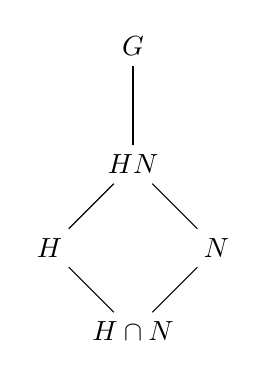
\begin{tikzpicture}[node distance=1.5cm]
    \node (G) {$G$};
    \node[below of=G] (HN) {$HN$};
    \node[below right of=HN] (N) {$N$};
    \node[below left of=HN] (H) {$H$};
    \node[below right of=H] (HiN) {$H\cap N$};
    \draw (G) edge (HN)
          (HN) edge (H)
          (HN) edge[above right] node {$\trianglelefteq$} (N)
          (H) edge[below left] node {$\trianglelefteq$} (HiN)
          (N) edge (HiN);
\end{tikzpicture}
\end{center}

\begin{theorem}[Third Isomorphism Theorem] \label{thm:iso3}
    Let $G$ be a group and let $H,N$ be normal subgroups of $G$ such that $N \leq H$. Then, $(H/N) \trianglelefteq (G/N)$ and $G/H \cong \ddfrac{G/N}{H/N}$.
\end{theorem}
\begin{center}
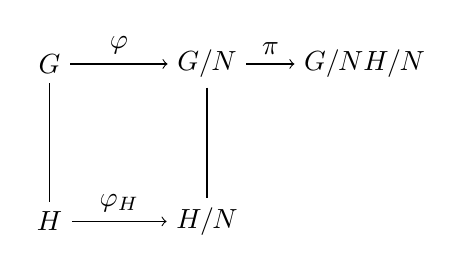
\begin{tikzpicture}[node distance=2cm]
    \node (G) {$G$};
    \node[below of=G] (H) {$H$};
    \node[right of=G] (G/N) {$G/N$};
    \node[below of=G/N] (H/N) {$H/N$};
    \node[right of=G/N] (GNHN) {$\ddfrac{G/N}{H/N}$};
    \draw   (G) edge[left] node {$\trianglelefteq$} (H)
            (G/N) edge[right] node {$\trianglelefteq$} (H/N);
    \path[->]
        (G) edge[above] node {$\varphi$} (G/N)
        (H) edge[above] node {$\varphi_H$} (H/N)
        (G/N) edge [above] node {$\pi$} (GNHN);
\end{tikzpicture}
\end{center}
\begin{proof}
    We will use the above diagrammatic representation to prove this theorem. $\varphi \colon G \to G/N$ represents the natural homomorphism $\varphi(g) = gN$. $\varphi_H$ is the restriction of $\varphi$ to $H$. Let $X \in H/N$ and $Y \in G/N$. We have $X = hN$ for some $h \in H$ and $Y = gN$ for some $g \in G$. Now,
    \[
        YXY^{-1} = (gN)(hN)(g^{-1}N) = (ghg^{-1})N
    \]
    Since $H \trianglelefteq G$, we have that $ghg^{-1} = h^{\prime}$ for some $h^{\prime} \in H$. Thus, $YXY^{-1} = h^{\prime} N \in H/N$ and hence, $H/N \trianglelefteq G/N$. Consider the map $\pi \circ \varphi \colon G \to \ddfrac{G/N}{H/N}$. Since $\pi$ and $\varphi$ are surjective homomorphisms, $\pi \circ \varphi$ is also a surjective homomorphism. We know that $\ker\pi = H/N$. Thus, $\ker(\pi\circ\varphi) = \left\{ g \in G \mid \varphi(g) = H/N \right\}$. Thus, $\ker(\pi\circ\varphi) = H$. By the \nameref{thm:iso1}, we conclude that
    \[
        G/H \cong \frac{G/N}{H/N} \qedhere
    \]
\end{proof}


\begin{theorem} \label{thm:abelian-subgroup-of-order-divisor}
    Let $G$ be a finite abelian group of order $n$ and let $d \in \N^+$ be such that $d \divides n$. Then, $G$ has a subgroup of order $d$.
\end{theorem}
\begin{proof}
    We will apply induction on the order of $G$. If $n = 1$, the theorem is true. Suppose the theorem is true for all abelian groups of order strictly less than $n$. We first prove that for any prime $p$ with $p \divides n$, $G$ has an element of order $p$.
    
    \medskip
    
    We may assume $\abs{G} > 1$. Suppose $a \in G$ such that $\abs{a} = m \geq 2$. Suppose $p \divides m$. Then, $a^{m/p}$ has order $p$. Suppose $p \notdivides m$. Consider $N = \langle a \rangle$ with $\abs{N} = m$. Since $G$ is abelian, every subgroup of $G$ is normal. Hence, $N \trianglelefteq G$. Now, consider the quotient group $G/N$. We know that $\abs{G/N} = n/m$. Since $p \divides n$ and $p \notdivides m$, we conclude that $p$ divides $\abs{G/N}$. By the induction hypothesis, there exists an element of order $p$ in $G/N$, since $G/N$ is abelian and of order strictly less than $n$. Thus, $\abs{bN} = p$ for some $b \in G$. Suppose $\abs{b} = k$. This gives us $b^k = 1 \implies (bN)^k = N$. Thus, $p \divides k$ and we are back to the first case. Hence, there is an element of order $p$ and hence a subgroup of order $p$.
    
    \medskip
    
    Fix a prime $p$ such that $p \divides d$. Let $a \in G$ be an element of order $p$ in $G$ and let $N = \langle a \rangle$. Thus, $\abs{N} = p$. We have $\abs{G/N} = n/p < n$. Now, by the induction hypothesis, there exists a subgroup $H/N$ of $G/N$ with $\abs{H/N} = d/p$. Thus, $\abs{H}/\abs{N} = d/p$, which gives us $\abs{H} = d$ and we are done.
\end{proof}
\section{Group Actions}

\subsection{Definitions}

\begin{defn}[Group Action]
    Let $G$ be a group and let $S$ be a set. A \deff{group action of $G$ on $S$} is a map from $G \times S$ to $S$ (denoted as $g\cdot s$ for all $g \in G$, $s \in S$) satisfying
    \begin{enumerate}
        \item $g \cdot (h \cdot s) = (gh) \cdot s$ for all $g,h \in G$, $s \in S$.
        \item $1 \cdot s = s$ for all $s \in S$.
    \end{enumerate}
    In this case, we say that $G$ \deff{acts} on $S$ or that $S$ is a \deff{$G$-set}.
\end{defn}

\begin{defn}[Permutation Representation]
    Let $G$ be a group and let $S$ be a set. A homomorphism $\varphi \colon G \to S_S$ is called a \deff{permutation representation of $G$ on $S$}.
\end{defn}

\begin{theorem} \label{thm:action-gives-permutation}
    Let $G$ be a group and let $S$ be a set. Define $\sigma_g \colon S \to S$ with $\sigma_g(s) = g\cdot s$ for all $s \in S$. Then, the following is true.
    \begin{enumerate}
        \item $\sigma_g$ is a bijection, and hence a permutation of $S$.
        \item The map $\varphi \colon G \to S_S$ defined by $\varphi(g) = \sigma_g$ is a permutation representation of $G$ on $S$.
    \end{enumerate}
\end{theorem}
\begin{proof}
    To prove the first part, we show that $\sigma_{g^{-1}}$ is the inverse of $\sigma_g$. Indeed, we have
    \[
        \sigma_{g^{-1}} \circ \sigma_g (s) = g^{-1} \cdot (g \cdot s) = (g^{-1}g) \cdot s = 1\cdot s = s \text{ for all }s\in S
    \]
    Similarly, $\sigma_g$ is the inverse of $\sigma_{g^{-1}}$. This shows that $\sigma_g$ is a bijection, and hence a permutation of $S$. 
    
    We already know that $1\cdot s = s$ for all $s \in S$. To prove that $\varphi$ as defined above is a homomorphism, we see that
    \[
        \sigma_g\circ \sigma_h(s) = g \cdot (h \cdot s) = (gh) \cdot s = \sigma_{gh}(s) \text{ for all }g,h \in G, s \in S
    \]
    Hence, $\varphi(g)\varphi(h) = \varphi(gh)$ for all $g,h \in G$. 
\end{proof}

It turns out that the converse of the above theorem is also true. 
\begin{prop} \label{prop:permutation-gives-action}
    Let $G$ be a group and let $S$ be a set. Let $\psi \colon G \to S_S$ be a permutation representation of $G$ on $S$. Then, the map from $G \times S$ to $S$, defined by
    \[
        g\cdot s = \psi(g)(s) \text{ for all }g\in G, s \in S
    \]
    is a group action of $G$ on $S$.
\end{prop}
\begin{proof}
    Clearly, $\psi(1)$ is the identity permutation and hence $1\cdot s = s$ for all $s \in S$. We have
    \[
        g\cdot(h\cdot s) = \psi(g)\left( \psi(h)(s) \right)
    \]
    Since $\psi$ is a group homomorphism, we get
    \[
        g \cdot(h \cdot s) = \psi(gh)(s) = (gh) \cdot s \qedhere
    \]
\end{proof}

\begin{exe}
    \phantom{hi}
    \begin{enumerate}
        \item Consider $S = G$. The map $\psi \colon G \times G \to G$ defined by $(g,h) \mapsto gh$, is a group action. The permutation representation induced by this group action is the map from $G$ to $S_G$ defined by $g \mapsto T_g$, where $T_g$ is the translation map, defined by $T_g(h) = gh$. Moreover, the kernel of this permutation representation is trivial, and hence is an injective group homomorphism from $G$ to $S_G$. Hence, $G$ is isomorphic to a subgroup of $S_G$, which is precisely Cayley's Theorem (\Cref{thm:cayley}).
        
        \item Again, consider $S = G$. The map $\psi \colon G \times G \to G$ defined by $(g,h) \mapsto ghg^{-1}$ is also a group action. The permutation induced by this group action is the map from $G$ to $S_G$ defined by $g \mapsto \gamma_g$, where $\gamma_g$ is the conjugation map, defined by $\gamma_g(h) = ghg^{-1}$. The kernel of this permutation is the set 
        \[
            \left\{ g \in G \mid ghg^{-1} = h \text{ for all } h \in G \right\}
        \]
        which is precisely the center of $G$, $Z(G)$. By the First Isomorphism Theorem (\Cref{thm:iso1}), we get
        \[
            G/Z(G) \cong \left\{ \gamma_g \mid g \in G \right\}.
        \]
        The group on the right is the group of inner automorphisms of $G$.
        
        \item Let $\F$ be a field. The group $GL_n(\F)$ acts on the $n$-dimensional vector space $V \vcentcolon= \F^n$ with the group action naturally defined from $GL_n(\F) \times V \to V$ as 
        \[
            (A, u) \mapsto Au \text{ (the matrix product).}
        \]
        In the case that the field is $\F_2$, the vector space $V = \F^2$ has precisely $4$ vectors, given by
        \[
            V = \left\{ \begin{bmatrix}
            0 \\ 0
            \end{bmatrix} \, , \, \underbrace{\begin{bmatrix}
            1 \\ 0
            \end{bmatrix}}_{e_1}\, , \, \underbrace{\begin{bmatrix}
            0 \\ 1
            \end{bmatrix}}_{e_2}\, , \, \underbrace{\begin{bmatrix}
            1 \\ 1
            \end{bmatrix}}_{e_1+e_2} \right\}
        \]
        Now, consider $S = \{ e_1, e_2, e_1+e_2\}$ and consider $G = GL_2(\F_)$ with the group action defined as above. This group action gives rise to a permutation representation from $G$ to $S_3$ (since $S$ has three elements) defined by $A \mapsto L_A$, where $L_A$ is the \emph{linear map} induced by $A$, defined by $L_A(u) = Au$. The kernel of this permutation representation is trivial and hence, is an injective group homomorphism. Moreover, since $\abs{GL_2(\F_2)} = \abs{S_3} = 6$, we must have that this homomorphism is also onto, and hence an isomorphism. Thus, $GL_2(\F_2) \cong S_3$.
    \end{enumerate}
\end{exe}

\subsection{Orbits and Stabilisers}

\begin{defn}
    Let $G$ be a group and let $S$ be a set. Let $\cdot \colon G \times S \to S$ be a group action. For a fixed $s \in S$, we define the \deff{orbit} of $s$ under this group action as
    \[
        O_s \vcentcolon= \left\{ g \cdot s \mid g \in G \right\}.
    \]
\end{defn}
\begin{defn}
    Let $G$ be a group and let $S$ be a set. Let $\cdot \colon G \times S \to S$ be a group action. For a fixed $s \in S$, we define the \deff{stabiliser} of $s$ under this group action as
    \[
        G_s \vcentcolon= \left\{ g \in G \mid g \cdot s = s \right\}.
    \]
\end{defn}
Note that $O_s \subseteq S$ and $G_s \leq G$. 

\begin{defn}
    Let $G$ be a group and let $S$ be a set. Let $\cdot \colon G \times S \to S$ be a group action. The group is said to act \deff{transitively} on $S$ (via the action $\cdot$) if $O_s = S$ for all $s \in S$. That is, for every pair $s,t \in S \times S$, there exists $g \in G$ such that $g \cdot s = t$. 
\end{defn}

\begin{prop} \label{prop:same-orbit-equivalence}
    Let $G$ be a group and let $S$ be a set. Let $\cdot \colon G \times S \to S$ be a group action. Define a relation $\sim$ on $S$ defined by $s \sim s^{\prime}$ if $s^{\prime} = g \cdot s$ for some $g \in G$. Then, $\sim$ is an equivalence relation. In other words, $s^{\prime} \sim s$ if $s^{\prime} \in O_s$.
\end{prop}
\begin{proof}
    Note that $s \sim s$ since $s = 1 \cdot s$, hence $\sim$ is reflexive. If $s \sim s^{\prime}$, then $s^{\prime} = g \cdot s$ for some $g \in G$. We then have
    \[
        g^{-1} \cdot s^{\prime} = g^{-1} \cdot g \cdot s = (g^{-1}g) \cdot s = 1 \cdot s = s \implies s \sim s^{\prime}.
    \]
    Hence, $\sim$ is symmetric. If $s \sim s^{\prime}$ and $s^{\prime} \sim s^{\prime\prime}$, we have that $s^{\prime} = g \cdot s$ and $s^{\prime\prime} = h \cdot s^{\prime}$ for some $g,h \in G$. Now, 
    \[
        s^{\prime\prime} = h \cdot s^{\prime} = h \cdot (g \cdot s) = (hg) \cdot s \implies s \sim s^{\prime\prime} \text{ since $hg \in G$.}
    \]
    Hence, $\sim$ is also transitive, and thus an equivalence relation.
\end{proof}
\begin{cor}
Let $G$ be a group and let $S$ be a set. Let $\cdot \colon G \times S \to S$ be a group action. Then, $S$ can be written as a disjoint union of orbits.
\end{cor}
\begin{proof}
    This follows trivially from \Cref{prop:same-orbit-equivalence} and \Cref{prop:equivalence-partition}.
\end{proof}

\begin{theorem}[Orbit-Stabiliser Formula] \label{thm:orbit-stabiliser}
    Let $G$ be a group and let $S$ be a set. Let $\cdot \colon G \times S \to S$ be a group action. Let $G/G_s$ denote the set\footnotemark\ of cosets of the stabiliser of an element $s \in S$. Then, $\varphi \colon G/G_s \to O_s$ defined by
    \[
        \varphi(gG_s) \vcentcolon= g \cdot s
    \]
    is a bijection. In particular, $\abs{O_s} = [G \colon G_s]$, where $[G \colon G_s] \vcentcolon= \abs{G/G_s}$ is the \emph{index} of $G_s$ in $G$. In the case that $G$ is finite, we have $[G \colon G_s] = \abs{G} / \abs{G_s}$.
\end{theorem}
\footnotetext{Note that in general $G_s$ need not be a normal subgroup of $G$. However, we can still talk about its set of cosets.}
\begin{proof}
    We first show that this map is well-defined by noting that
    \[
        gG_s = hG_s \iff h^{-1}g \in G_s \iff (h^{-1}g) \cdot s = s \iff g\cdot s = h\cdot s.
    \]
    Note that this also proves that $\varphi$ is injective. $\varphi$ is also trivially surjective, and hence a bijection. 
\end{proof}

\begin{prop}
    Let $G$ be a group and let $S$ be a set. Let $\cdot \colon G \times S \to S$ be a group action. Let $s \in S$ and $g \in G$. Then, $G_{g \cdot s} = g G_s g^{-1}.$
\end{prop}
\begin{proof}
    We have 
    \[
        h \in G_{g \cdot s} \iff h \cdot (g \cdot s) = g \cdot s \iff (g^{-1}hg) \cdot s = s \iff g^{-1}hg \in G_s \iff h \in gG_sg^{-1}.
    \]
\end{proof}

\begin{cor} \label{cor:|S|-in-terms-of-indices-of-stabilisers}
    Let $G$ be a group and let $S$ be a set. Let $\cdot \colon G \times S \to S$ be a group action. Then, 
    \[
        \abs{S} = \sum_{s_i} \, \left[ G \colon G_{s_i} \right]
    \]
    where the sum runs over one element $s_i$ from each orbit of $S$. 
\end{cor}

\begin{defn}
    Let $G$ be a group and let $g \in G$. We define the \deff{centraliser} of $g$ as
    \[
        Z(g) \vcentcolon= \left\{ h \in G \mid gh = hg \right\}.
    \]
    Moreover, the centraliser $Z(g)$ is a subgroup of $G$.
\end{defn}

\begin{defn}
    Let $G$ be a group and let $H$ be a subgroup of $G$. We define the \deff{normaliser} of $H$ as
    \[
        N(H) \vcentcolon= \left\{ g \in G \mid gH = Hg \right\}.
    \]
\end{defn}
\begin{prop} \label{prop:normaliser-properties}
    Let $G$ be a group and let $H$ be a subgroup of $G$. Then, $H \trianglelefteq N(H)$ and $N(H)$ is the largest subgroup of $G$ in which $H$ is a normal subgroup. 
\end{prop}



\begin{theorem} \label{thm:cardinality-of-conjugacy}
    Let $G$ be a finite group and let $g \in G$. Let $C(g)$ be the conjugacy class of $g$, and let $Z(g)$ be the centraliser of $g$. Then, 
    \[
        \abs{G} = \abs{C(g)} \cdot \abs{Z(g)}
    \]
\end{theorem}
\begin{proof}
    Consider $G$ acting on $G$ via conjugation. That is, consider the group action $\cdot \colon G \times G \to G$, defined by $(h,g) \mapsto hgh^{-1}$. In this case, $O_g$ is clearly the conjugacy class, $C(g)$, of $g$, and $G_g$ is the centraliser, $Z(g)$, of $g$. Applying the \nameref{thm:orbit-stabiliser} gives us the required result.
\end{proof}

\begin{cor} \label{cor:|S|-in-terms-of-conjugacy}
Let $G$ be a finite group. Then, 
\[
    \abs{G} = \sum_{g}\, \abs{C(g)}
\]
where the sum runs over one element from each conjugacy class of $G$.
\end{cor}
\begin{proof}
    This follows directly by applying \Cref{thm:cardinality-of-conjugacy} to \Cref{cor:|S|-in-terms-of-indices-of-stabilisers}.
\end{proof}

\begin{cor}[Class Equation] \label{cor:class-equation}
    Let $G$ be a group and let $Z(G)$ be its center. Then, 
    \[
        \abs{G} = \abs{Z(G)} + \sum_{g} \, \left[ G \colon Z(g) \right]
    \]
    where the sum runs over one element from each conjugacy class that is not in the center.
\end{cor}
\begin{proof}
    The proof trivially follows from \Cref{cor:|S|-in-terms-of-conjugacy} once we note that each element of the center $Z(G)$ forms a conjugacy class containing only itself.
\end{proof}

\begin{defn}
    Let $G$ be a finite group and let $p$ be a prime. $G$ is called a \deff{$p$-group} if $\abs{G} = p^n$ for some $n \in \N^+$.
\end{defn}

\begin{theorem} \label{thm:p-group-has-non-trivial-center}
    If $G$ is a $p$-group, then $\abs{Z(G)} \geq p$. In particular, every $p$-group has a non-trivial center. 
\end{theorem}
\begin{proof}
    By the \nameref{cor:class-equation} of $G$, we have
    \[
        p^n = \abs{Z(G)} + \sum_{g} \, \left[ G \colon Z(g) \right]
    \]
    Note that in the sum to the right, each index is at least $2$ (since the sum varies over only non-trivial conjugacy classes). However, $\left[ G \colon Z(g) \right]$ must divide $\abs{G} = p^n$. It follows that each index is a power of $p$, and hence, $\abs{Z(G)}$ is also a power of $p$. Hence, $\abs{Z(G)} \geq p$. 
\end{proof}
In the case that $G$ is abelian, $Z(G)$ is the entire group $G$. However, the above theorem is truly powerful for non-abelian groups as it states that every non-abelian $p$-group has a non-trivial proper normal subgroup, namely, its center. 

\begin{theorem}
    Let $G$ be a $p$-group and let $\abs{G} = p^n$. Then, there is a sequence of subgroups $H_i$ such that $\abs{H_i} = p^i$ for $i = 1, \ldots, n$. Moreover,
    \begin{enumerate}
        \item $1 \trianglelefteq H_1 \trianglelefteq \ldots \trianglelefteq H_n$, and 
        \item $(H_1 \cong) \, H_1 / 1 , H_2/H_1, \ldots, H_n/H_{n-1}$ are all cyclic groups of order $p$.
    \end{enumerate}
    Here, $1$ represents the trivial subgroup of $G$.
\end{theorem}
\begin{proof}
    We apply induction on $n$. If $n = 1$, the theorem is trivially true. Suppose the theorem holds for groups of order $p^{n-1}$ ($n > 1$). Let $x \in Z(G)$ and $x \neq 1$ (such an $x$ exists since the center is non-trivial, by \Cref{thm:p-group-has-non-trivial-center}). Moreover, $\abs{x} = p^r$ where $r < n$ (why?). We also have $\abs{x^{p^{r-1}}} = p$. Define $y \vcentcolon= x^{p^{r-1}}$ and let $H = \langle y \rangle$. We have $H \trianglelefteq G$. Now, consider the quotient group $G/H$, of order $p^{n-1}$. By the induction hypothesis, $G/H$ has a sequence of subgroups as follows.
    \[
        1 \, \trianglelefteq \, H_2/H \, \trianglelefteq \, H_3/H \, \trianglelefteq \, \ldots \, \trianglelefteq \, H_n/H = G/H.
    \]
    By the \nameref{thm:correspondence}, we may conclude the result.
\end{proof} 

\begin{defn}
    A \deff{simple group} is a non-trivial group that has no non-trivial normal subgroups.
\end{defn}
\begin{prop}
    The alternating group $A_5$ is simple.
\end{prop}
\begin{proof}
    We have $\abs{A_5} = 60$. Let the elements
    \[
        (1), \, \underbrace{(1 \, 2 \, 3)}_{\sigma}\, , \, \underbrace{(1 \, 2 \, 3 \, 4 \, 5)}_{\tau} \, , \, \underbrace{(1\, 2)(3\, 4)}_{\alpha}
    \]
    be representative elements of the conjugacy classes in $A_5$. Clearly, $\abs{C(1)} = 1$. By the \nameref{thm:orbit-stabiliser}, 
    \[
        \abs{C(\sigma)} = \frac{60}{\abs{Z(\sigma)}}.
    \]
    Now, the elements in the centraliser of $\sigma$ in $A_5$ are the powers\footnotemark\ of $\sigma$, of which there are precisely three - $(1), \sigma,$ and $\sigma^2$. Thus, $\abs{C(\sigma)} = 20$. Similarly, $\abs{C(\tau)} = 12$. Since the number of $5$-cycles in $A_5$ is $24$, there is another $5$-cycle, say $\gamma$, that lies outside of $C(\tau)$ and has its own conjugacy class of $12$ elements. That is, $\abs{C(\gamma)} = 12$. Elementary combinatorics shows that there are $15$ permutations having structure $(1 \, 2)(3 \, 4)$. Moreover, all such elements lie in the same conjugacy class (why?). We then have $\abs{C(\alpha)} = 15$, so that the class equation of $A_5$ becomes
    \[
        60 = 1 + 12 + 12 + 15 + 20.
    \]
    Now, suppose $A_5$ had a non-trivial normal subgroup, say $H$. Then, $H$ must be a disjoint union of conjugacy classes of $A_5$ and must contain the identity (the center). Moreover, $\abs{H}$ must divide $60$. However, from the class equation, we can verify that no possible combination of conjugacy classes along with the center has order that is a divisor of $60$. Hence, $A_5$ is a simple group. 
\end{proof}
\footnotetext{Note that the two cycle $(4 \, 5)$ also permutes with $\sigma$ but it is an odd permutation, hence not an element of $A_5$.}

\begin{rem}
    The simplicity of $A_5$ is crucial in proving that there is a quintic polynomial that is not solvable by radicals.
\end{rem}

\begin{lem} \label{lem:every-even-permutation-as-prod-of-3-cycles}
    Let $n \geq 3$. Any even permutation in $S_n$ can be written as a product of $3$-cycles. 
\end{lem}
\begin{proof}
    We leave the proof as an exercise to the reader. The proof should be fairly trivial after noting the following identities.
    \[
        (a \, b)(b \, c) = (a \, b \, c) \text{ and } (a \, b)(c \, d) = (a \, b \, c)(b \, c \, d).
    \]
\end{proof}

\begin{theorem}[Galois]
    $A_n$ is simple for all $n \geq 5$.
\end{theorem}
\begin{proof}
    Let $n \geq 5$. Suppose that there is a non-trivial normal subgroup of $A_n$, that is, there is a normal subgroup $N \trianglelefteq A_n$ such that $N \neq (1)$ and $N \neq A_n$. Recall that a fixed point of a permutation is a point that is not `moved' by the permutation. Among all the permutations in $A_n \setminus (1)$, pick a permutation $\sigma$ that has the maximum number of fixed points. We will show that $\sigma$ must be a $3$-cycle. First, we write $\sigma$ as a product of disjoint cycles. 
    \[
        \sigma = (a_1 \, \ldots \, a_k) (b_1 \, \ldots \, b_m) \cdots
    \]
    Suppose $k < m$. Then, observe that $\sigma^k$ is a nontrivial permutation in $A_n$ that has strictly more fixed points than $\sigma$, which is a contradiction. Similarly, $k$ cannot be strictly greater than $m$, and hence, by trichotomy, we conclude that $k = m$. Proceeding this way, we see that $\sigma$ has to decompose as a product of cycles of equal length, say $m$. Suppose $m = 2$. Then, $\sigma$ is a product of transpositions. Since $\sigma$ is an even permutation, there must be an even number of transpositions in the decomposition. Moreover, since $\sigma$ is non-trivial, we must have at least one (and hence, at least two) transpositions. Thus, 
    \[
        \sigma = (a_1 \, a_2)(a_3 \, a_4) \cdots (a_{2r-1} \, a_{2r})
    \]
    with $r \geq 2$. Since $n \geq 5$, there exists a $b \neq a_1, a_2, a_3, a_4$. Let $\tau = (a_3 \, a_4 \, b)$. Define the \emph{commutator} of $\tau$ with $\sigma$ as $\gamma \vcentcolon= \tau\sigma\tau^{-1}\sigma^{-1}$. Since $\sigma \in N$ and $N$ is normal, we conclude that $\gamma \in N$. The fixed points of $\sigma$ are carried over to $\gamma$. That is, $\sigma(j) = j \implies \gamma(j) = j$. Moreover, $a_1$ and $a_2$, which were not fixed points of $\sigma$, have become fixed under $\gamma$. Thus, $\gamma$ has strictly more fixed points than $\sigma$, which is a contradiction. Hence, $m \neq 2$ and $m \geq 3$. 
    
    We again consider the decomposition
    \[
        (a_1 \, \ldots \, a_m)(b_1 \, \ldots \, b_m) \cdots
    \]
    where $m$ is now at least $3$. Suppose $\sigma$ is not a $3$-cycle. Then, choose distinct $r,s \neq a_1, a_2, a_3$ (this is again possible since $n \geq 5$). Now, consider $\tau = (a_3 \, r \, s) \in A_n$ and the commutator $\gamma = \tau\sigma\tau^{-1}\sigma^{-1}$. As before, we have $\gamma \in N$. We may again verify that $\gamma$ preserves the fixed points of $\sigma$, and that $\gamma(a_2) = a_2$. Hence, $\gamma$ has strictly more fixed points than $\sigma$, which is a contradiction. Hence, $\sigma$ must be a $3$-cycle in which case it generates the entire group $A_n$ by \Cref{lem:every-even-permutation-as-prod-of-3-cycles}, and $N = A_n$. Thus, a nontrivial subgroup $N$ cannot exist, and hence $A_n$ is simple for $n \geq 5$. 
\end{proof}
\section{Sylow Theorems}

\begin{theorem}[Cauchy's Theorem] \label{thm:cauchy}
    Let $G$ be a finite group and let $p$ be a prime. If $p$ divides the order of $G$, then $G$ has a subgroup of order $p$. 
\end{theorem}
\begin{proof}
    Consider the set
    \[
        S = \left\{ (x_1, \ldots , x_p) \in G^p \mid x_1 \cdots x_p = 1 \right\}.
    \]
    \[
        \left( \sigma, (x_1, \ldots, x_p) \right) \longmapsto \left( x_{\sigma(1)}, \ldots, x_{\sigma(p)} \right)
    \]
    for all $\sigma \in H$ and  $(x_1, \ldots, x_p) \in S$. Notice that the orbit of the $(1, \ldots, 1)$ is itself. Since $S$ can be written as a disjoint union of orbits, it follows that there is at least another orbit that has only one element (this follows from divisibility considerations, since $p$ divides $\abs{S}$). Thus, there exists a $p$-tuple $(x_1, \ldots, x_p) \neq (1, \ldots, 1)$ such that $O((x_1, \ldots, x_p)) = \left\{ (x_1, \ldots, x_p) \right\}$. Since the orbit of this tuple contains only itself, and since permutations in $H$ cyclically permute the elements of the tuple, it follows that each element of the tuple. That is, such an element of the form $(x, \ldots, x)$ for some $x \in G$ with $x \neq 1$. Since $(x, \ldots, x) \in S$, it follows that $x^p = 1$. It then follows that $\abs{x} = p$, and the cyclic subgroup $\langle x \rangle$ is a subgroup of $G$ of order $p$. 
\end{proof}

\begin{prop} \label{prop:p^n-has-normal-subgroups-p^i}
    Let $G$ be a finite group of order $p^n$ where $p$ is a prime and $n \in \N^+$. Then, there are normal subgroups
    \[
        \left\{ 1 \right\} = G_0 < G_1 < \ldots < G_n = G
    \]
    such that $\abs{G_i} = p^i$ and $G_i \trianglelefteq G$ for $i = 0, \ldots, n$.
\end{prop}

\begin{proof}
    We prove this by induction on $n$. In the case that $n=1$, we trivially have $G_0 = \{1\}$ and $G_1 = G$. Now, assume that $n \geq 2$ and that the result holds for $n-1$. By \Cref{thm:p-group-has-non-trivial-center}, $G$ has a non-trivial center, and $p$ divides $\abs{Z(G)}$. By \nameref{thm:cauchy}, $Z(G)$ has an element of order $p$, say $z$. We define $G_1 = \langle z \rangle$. Clearly, $\abs{G_1} = p$. Moreover, since $G_1 \leq Z(G)$ and $Z(G) \trianglelefteq G$, we conclude that $G_1 \trianglelefteq G$. Now, define $H = G/G_1$. We have $\abs{H} = p^n/p = p^{n-1}$. By the induction hypothesis, $H$ has normal subgroups
    \[
        \left\{ 1 \right\} = H_0 < H_1 < \ldots < H_{n-1} = H
    \]
    such that $\abs{H_i} = p^i$ and $H_i \trianglelefteq H$ for $i = 0, \ldots, n-1$. By the \nameref{thm:correspondence}, there is a normal subgroup $G_{i+1}$ of $G$ such that $G_{i+1}/G_1 = H_i$ for $i =0, \ldots, n-1$. Moreover, $\abs{G_{i+1}} = \abs{G_1} \cdot \abs{H_i} = p^{i+1}$ for $i=0, \ldots, n-1$. We also have that $G_i \leq G_{i+1}$ by the \nameref{thm:correspondence}. This concludes the proof.
\end{proof}

\begin{defn}
    Let $G$ be a group and let $H \leq G$ be a subgroup. If $\abs{H} = p^i$ for a prime $p$ and some positive integer $i$, then $H$ is called a \deff{$p$-subgroup} of $G$.
\end{defn}

\begin{defn}
    Let $G$ be a finite group and $\abs{G} = p^n m$ where $p$ is a prime, $n$ is a positive integer, and $\gcd(p,m) = 1$. A subgroup of $G$ having order $p^n$ is called a \deff{Sylow $p$-subgroup} of $G$. The set of all Sylow $p$-subgroups of $G$ is denoted as $\Syl_p(G)$. The number of Sylow $p$-subgroups of $G$ is denoted as $n_p \vcentcolon= \abs{\Syl_p(G)}$.
\end{defn}

\begin{theorem}[Sylow Theorems] \label{thm:sylow}
Let $G$ be a finite group and $\abs{G} = p^n m$ where $p$ is a prime, $n$ is a positive integer, and $\gcd(p,m) = 1$. Then, the following are true.
\begin{enumerate}
    \item $G$ has subgroups of order $p^i$ for $i = 1, \ldots, n$. In particular, $G$ has a Sylow $p$-subgroup, that is, $n_p \geq 1$.
    \item Any $p$-subgroup of $G$ is contained in a Sylow $p$-subgroup of $G$.
    \item Any two Sylow $p$-subgroups of $G$ are conjugates of each other. 
    \item $n_p \equiv 1 \Mod{p}$ and $n_p \divides m$. 
\end{enumerate}
\end{theorem}

\begin{proof}
    \phantom{hi}
    \begin{enumerate}
        \item When $\abs{G} = 1$, the statement is trivially true. Now, assume that the statement is true for all finite groups of order less than $\abs{G}$. The class equation of $G$ is
        \[
            \abs{G} = \abs{Z(G)} + \sum_{g} \left[ G \colon Z(g) \right]
        \]
        where the sum runs over one representative from each conjugacy class that is not the center. Suppose that $p \notdivides \abs{Z(G)}$. Since $p$ divides $\abs{G}$, there exists a $g$ in the second sum such that $p \notdivides \abs{G}/\abs{Z(g)}$. Since $p^n$ divides the order of $G$, it follows that $p^n$ divides $\abs{Z(g)}$. Note that $Z(g)$ is not the whole group since $g$ is not a central element. Hence, $\abs{Z(g)} < \abs{G}$. From the induction hypothesis, it follows that $Z(g)$ has subgroups of order $p^i$ for $i = 1, \ldots, n$ and in particular, a Sylow $p$-subgroup. Since $Z(g) \leq G$, this result extends to $G$ as well. Now, if $p$ divides $Z(G)$, then by \nameref{thm:cauchy}, there exists an element $z \in Z(G)$ of order $p$. Let $H = \langle z \rangle$. Then, $H \trianglelefteq G$. We leave the rest of the proof as an exercise to the reader. The proof follows along similar lines as \Cref{prop:p^n-has-normal-subgroups-p^i}, by considering the quotient group $G/H$ (which has order strictly less than $\abs{G}$), proving the result there and pulling it back to $G$ by the \nameref{thm:correspondence}.
        
        \item Let $H^{\prime} \leq G$ and $\abs{H^{\prime}} = p^i$ for some $0 \leq i \leq n$. We must show that $H^{\prime}$ is contained in a Sylow $p$-subgroup of $G$. Suppose $H$ is a Sylow $p$-subgroup of $G$. Consider the set
        \[
            S = G/H = \left\{ gH \mid g \in G \right\}.
        \]
        We have $\abs{S} = \abs{G}/\abs{H} = m$. Let $H^{\prime}$ act on $S$ by translation, with action defined from $H \times S$ to $S$ as $(h, gH) \mapsto hgH$. We leave it to the reader to verify that this is indeed a group action. Now, $S$ is a disjoint union of $H^{\prime}$-orbits and thus 
        \[
            \abs{S} = \sum_{h} \, \abs{O_h}
        \]
        where the sum runs over one representative from each orbit. Note that each orbit must have cardinality of the form $p^k$ for $k=0, \ldots,i$, since $\abs{O}_h$ must divide $\abs{H}^{\prime}$ which is $p^i$. However, $\abs{S} = m$ and $p \notdivides m$. We hence conclude that there is at least one orbit that has only one element, that is, an orbit consisting of a single left coset, say $gH$. We thus have
        \begin{align*}
            &hgH = gH &\text{ for all } h \in H^{\prime} \\
            \implies &g^{-1}hg \in H &\text{ for all } h \in H^{\prime} \\
            \implies &g^{-1}H^{\prime}g \subseteq H \\
            \implies &H^{\prime} \subseteq gHg^{-1}
        \end{align*}
        Since $\abs{gHg^{-1}} = p^n$, $gHg^{-1}$ is also a Sylow $p$-subgroup of $G$. Hence, $H^{\prime}$ is contained in a Sylow $p$-subgroup of $G$.
        
        \item In the above, if $\abs{H}^{\prime} = p^n$, then we clearly have $H^{\prime} = gHg^{-1}$. Hence, any two Sylow $p$-subgroups are conjugates of each other.
        
        \item As defined earlier, $\Syl_p(G)$ denotes the set of all Sylow $p$-subgroups of $G$. $G$ acts on $\Syl_p(G)$ by conjugation, with action from $G \times \Syl_p(G)$ to $\Syl_p(G)$ defined as $(g,H) \mapsto gHg^{-1}$. Since every Sylow $p$-subgroup is a conjugate of a Sylow $p$-subgroup, there is only one orbit with respect to this group action, and hence, the group $G$ acts transitively on $\Syl_p(G)$. If $P$ is a Sylow $p$-subgroup, then $\Syl_p(G) = \left\{ gPg^{-1} \mid g \in G \right\}$. By the \nameref{thm:orbit-stabiliser}, 
        \[
            \abs{\Syl_p(G)} = \left[ G \colon G_P \right] = \frac{\abs{G}}{\abs{G_P}}.
        \]
        Now, 
        \[
            G_P = \left\{ g \in G \mid gPg^{-1} = P \right\} = N(P).
        \]
        Since $N(P)$ contains $P$, $\abs{N(P)} \geq p^n$. Now, the orbit-stabiliser formula immediately tells us that $\abs{\Syl_p(G)} = n_p \divides m$. Now, it remains to show that $n_p \equiv 1 \Mod{p}$.
        
        Now, we consider the Sylow $p$-subgroup, $P$, act on $\Syl_p(G)$ with the same action as defined as above. Now, $P \in \Syl_p(G)$ and $O_P = \left\{ P \right\}$. Suppose $Q \in \Syl_p(G)$, $Q \neq P$ with $O_Q = \left\{ Q \right\}$. Now, 
        \[
            O_Q = \left\{ gQg^{-1} \mid g \in P \right\} = \left\{ O_Q \right\} \iff gQg^{-1} = Q \text{ for all } g \in P
        \]
        Thus, $P \subseteq N(Q)$, and thus $P \leq N(Q)$. Moreover, $Q \trianglelefteq N(Q)$ by \Cref{prop:normaliser-properties}. By \Cref{prop:HK}, $PQ \leq N(Q)$. Since $Q \trianglelefteq N(Q)$, we also have $Q \trianglelefteq PQ$. By the \nameref{thm:iso3},
        \[
            \frac{PQ}{Q} \cong \frac{P}{P \cap Q} \implies \abs{\frac{PQ}{Q}} = \abs{\frac{P}{P\cap Q}} = p^i \text{ for some } i.
        \]
        Thus, $\abs{PQ} = p^{i+n}$, which implies that $i = 0$ and $\abs{PQ} = p^n$. Since $P \leq PQ$ and $Q \trianglelefteq PQ$, and $\abs{P} = \abs{Q} = \abs{PQ}$, it follows that $P = Q = PQ$. The main conclusion is that when $P$ acts on $\Syl_p(G)$, there is only one singleton orbit. All other orbits have cardinality $p^i$ for some $i \geq 1$. Since $\Syl_p(G)$ is a disjoint union of these orbits, we may write out the cardinality of $\Syl_p(G)$ (which is $n_p$) as the sum of cardinalities of all disjoint orbits. Now, `modding' out by $p$ gives us $n_p \equiv 1 \Mod{p}.$ \qedhere
    \end{enumerate}
\end{proof}
\section{Classification of Groups}

\subsection{Isomorphism Classes of Groups}

We now classify all groups of order at most $13$ using the Sylow theorems, along with some other specific orders.

\begin{prop}
    Let $p$ be a prime. Up to isomorphism, there is exactly one group of order $p$, namely the cyclic group $C_p$.
\end{prop}
\begin{proof}
    We leave the proof as an exercise to the reader. (Hint: \nameref{thm:lagrange}). 
\end{proof}

\begin{theorem} \label{thm:class-prime-square}
    Let $p$ be a prime. Up to isomorphism, there are only two groups of order $p^2$, namely, the cyclic group $C_{p^2}$, and the group $C_p \times C_p$. 
\end{theorem}
\begin{proof}
    Let $\abs{G} = p^2$ and let $Z(G)$ be the center of $G$. We first show that $G$ must be abelian. By \Cref{thm:p-group-has-non-trivial-center}, $Z(G)$ is non-trivial. By \nameref{thm:lagrange}, $Z(G)$ must have order $p$ or $p^2$. If $Z(G)$ has order $p^2$, then $Z(G) = G$, so that $G$ is abelian. If $Z(G)$ has order $p$, then $G/Z(G)$ has order $p$. Hence, $G/Z(G)$ is cyclic and hence abelian. However, this forces $G$ to be abelian, in which case $Z(G) = G$ and $\abs{Z(G)} = p^2$, which is a contradiction. Hence, $G$ is abelian. 
    
    Now, suppose there was an element of order $p^2$ in $G$. Then, $G \cong C_{p^2}$. If not, then all elements (except identity) have order $p$. Let $x$ be one such element. Now, choose $y \notin \langle x \rangle$. Both $\langle x \rangle$ and $\langle y \rangle$ are normal subgroups of $G$, intersecting trivially. By \Cref{prop:HK}, the cardinality of their product matches the cardinality of $G$. Hence, $G$ is the internal direct product of $\langle x \rangle$ and $\langle y \rangle$, both of which are isomorphic to $C_p$. \Cref{thm:group-isomorphic-to-product} now tells us that $G \cong C_p \times C_p$.
\end{proof}
\begin{cor} \label{cor:class-4}
    Up to isomorphism, there are only two groups of order $4$, namely, the cyclic group $C_4$, and the Klein-four group $V$. 
\end{cor}
\begin{proof}
    By \Cref{thm:class-prime-square}, $C_4$ and $C_2 \times C_2$ are the only two groups of order $4$. Since $V$ is a group of order $4$, and $V$ is not isomorphic to $C_4$ (why?), we conclude that $V \cong C_2 \times C_2$. 
\end{proof}

\begin{prop} \label{prop:unique-sylow-not-simple}
    Let $G$ be a group of order $mp^n$ where $m >1$ and $p$ is prime. If $n_p = 1$, then $G$ is not simple.
\end{prop}
\begin{proof}
    Let $H$ be the \emph{unique} Sylow $p$-subgroup of $G$. $H$ is clearly a proper non-trivial subgroup of $G$ since $\abs{H} = p^n$ and $1 < p^n < mp^n$. Moreover, for any $g \in G$, $gHg^{-1}$ is a Sylow $p$-subgroup of $G$ by the third Sylow theorem. By uniqueness, $gHg^{-1} = H$ for all $g \in G$, so that $H$ is normal. Hence, $G$ is not simple.
\end{proof}

\begin{theorem} \label{thm:class-6}
    Up to isomorphism, there are only two groups of order $6$, namely the cyclic group of order $6$, $C_6$, and the group of permutations $S_3$.
\end{theorem}
\begin{proof}
    Let $\abs{G} = 6 = 2 \cdot 3$. By the first Sylow theorem, $G$ has a Sylow $2$-subgroup, say $H$, and a Sylow $3$-subgroup, say $K$. We will let $n_2$ denote the number of Sylow $2$-subgroups of $G$, and $n_3$ denote the number of Sylow $3$-subgroups of $G$. By the fourth Sylow theorem,
    \begin{align*}
        n_2 &\equiv 1 \Mod{2} \text{ and } n_2 \divides 3 \implies n_2 = 1 \text{ or } 3. \\
        n_3 &\equiv 1 \Mod{3} \text{ and } n_3 \divides 2 \implies n_3 = 1.
    \end{align*}
    Hence, there is a unique Sylow $3$-subgroup of $G$, which is $K$, that is a normal subgroup of $G$ by \Cref{prop:unique-sylow-not-simple}. If $n_2 = 1$, then $H$ is also normal in $G$. Moreover, $\abs{H} = 2$ and $H = C_2$, and $\abs{K} = 3$ and $K = C_3$. Note that $H$ and $K$ are two normal subgroups of $G$ that intersect only in identity. By \Cref{prop:HK}, we have
    \[
        \abs{HK} = \frac{\abs{H} \cdot \abs{K}}{\abs{H \cap K}} = \frac{2 \cdot 3}{1} = 6.
    \]
    Again, from \Cref{prop:HK}, we know that $HK \leq G$. However, $\abs{HK} = \abs{G}$ and hence $HK = G$. Thus, $G$ is an internal direct product of $H$ and $K$. But $H$ and $K$ are the unique cyclic groups $C_2$ and $C_3$. Hence, $G = C_2 C_3$. By \Cref{thm:group-isomorphic-to-product}, $G \cong C_2 \times C_3$. Now, since $2$ and $3$ are coprime, by \Cref{prop:product-of-cyclic} and \Cref{ex:C6} in particular, we get that $G \cong C_6$.
    
    Now, consider that $n_2 = 3$, that is, there are $3$ Sylow $2$-subgroups of $G$, say $H_1, H_2$ and $H_3$. Let $\Syl_2(G) = \left\{ H_1, H_2, H_3 \right\}$ and let $G$ act on $\Syl_2(G)$ by conjugation, with action defined from $G \times \Syl_2(G)$ to $\Syl_2(G)$ as
    \[
        (g,H) \longmapsto gHg^{-1} \text{ for all } g \in G, H \in \Syl_2(G).
    \]
    For a fixed $g \in G$, $\gamma_g \colon \Syl_2(G) \to \Syl_2(G)$ defined by $\gamma_g(H) = gHg^{-1}$ defines a permutation of $\Syl_2(G)$, a set with $3$ elements. Now, construct the natural homomorphism $\varphi \colon G \to S_3$ with $\varphi(g) = \gamma_g$. Now, 
    \[
        \ker\varphi = \left\{ g \in G \mid gH_ig^{-1} = H_i \text{ for all } H_i \in \Syl_2(G) \right\} = N(H_1) \cap N(H_2) \cap N(H_3).
    \]
    We leave it as an exercise to show that $\ker\varphi = \{1\}$. Hence, $\varphi$ is injective. Moreover, $\abs{G} = \abs{S_3} = 6$. Thus, $\varphi$ is a bijection, and $G \cong S_3$. 
\end{proof}

\begin{theorem} \label{thm:class-pq-pnmid-q-1}
    Let $p,q$ be distinct primes with $p < q$ and let $p \notdivides q-1$. Up to isomorphism, there's only one group of order $pq$, namely the cyclic group $C_{pq}$.
\end{theorem}
\begin{proof}
    Let $\abs{G} = pq$. By the first Sylow theorem, $G$ has a Sylow $p$-subgroup, say $H$, and a Sylow $q$-subgroup, say $K$. By the fourth Sylow theorem,
    \begin{align*}
        n_p \equiv 1 \Mod{p} \text{ and } n_p \divides q \implies n_p = 1 \text{ (since $p \notdivides q-1$)}. \\
        n_q \equiv 1 \Mod{q} \text{ and } n_q \divides p \implies n_q = 1.
    \end{align*}
    Thus there is a unique Sylow $p$-subgroup, $H$, and a unique Sylow $q$-subgroup, $K$. By \Cref{prop:unique-sylow-not-simple}, $H \trianglelefteq G$ and $K \trianglelefteq G$. Since they also intersect only in identity, by \Cref{prop:HK}, we again have
    \[
        \abs{HK} = \frac{\abs{H} \cdot \abs{K}}{\abs{H \cap K}} = pq
    \]
    and $HK \leq G$. Since $\abs{HK} = \abs{G}$, we conclude that $HK = G$. Thus, $G$ is an internal direct product of $H$ and $K$. But $H$ and $K$ are the unique cyclic groups $C_p$ and $C_q$. Hence, $G = C_p C_q$. By \Cref{thm:group-isomorphic-to-product}, $G \cong C_p \times C_q$. Since $q$ and $p$ are coprime, by \Cref{prop:product-of-cyclic}, $G \cong C_{pq}$.
\end{proof}

\begin{theorem} \label{thm:class-21}
    Up to isomorphism, there are only two groups of order $21$, namely, the cyclic group $C_{21}$ and the group presented as $\left\langle x,y \mid x^7 = y^3 = 1; \, yx = x^2y \right\rangle$. 
\end{theorem}
\begin{proof}
    Let $\abs{G} = 21 = 3 \cdot 7$. By the first Sylow theorem, $G$ has a Sylow $3$-subgroup, say $H$, and a Sylow $7$-subgroup, say $K$. By the fourth Sylow theorem,
    \begin{align*}
        n_3 &\equiv 1 \Mod{3} \text{ and } n_3 \divides 7 \implies n_3 = 1 \text{ or } 7. \\
        n_7 &\equiv 1 \Mod{7} \text{ and } n_7 \divides 3 \implies n_7 = 1.
    \end{align*}
    Thus, there is a unique Sylow $7$-subgroup, $K$, of $G$. By similar reasoning as before, $K \trianglelefteq G$. Again. if $n_3 = 1$, then there is only one Sylow $3$-subgroup of $G$. By similar reasoning as before, we get $G \cong C_{21}$ in this case. 
    
    Now let us assume $n_3 = 7$ and let $H$ be a Sylow $3$-subgroup of $G$. Since $K \trianglelefteq G$, it follows from \Cref{prop:HK} that $HK \leq G$. Since $H$ and $K$ intersect only in identity, we get $HK = G$ by similar reasoning. Now, since $\abs{H} = 3$ and $\abs{K} = 7$ are both prime, these are both isomorphic to cyclic groups of corresponding orders. Thus, $H = \langle y \rangle$ and $K = \langle x \rangle$ where $\abs{y} = 3$ and $\abs{x} = 7$. Now, since $K \trianglelefteq G$, we have
    \[
        yxy^{-1} \in K \implies yxy^{-1} = x^i \text{ for some }i.
    \]
    If $i = 1$, then $G$ becomes abelian. If $G$ were abelian then for any two Sylow $3$-subgroups $H$ and $H^{\prime}$, we have $gHg^{-1} = H^{\prime} \implies H = H^{\prime}$, by commutativity. Hence, if $G$ is abelian, there is a unique Sylow $3$-subgroup, but we have assumed $n_3 = 7$. Hence, $i \neq 1$. Now, 
    \begin{align*}
        yxy^{-1} = x^i \implies y^2xy^{-2} &= y(yxy^{-1})y^{-1} = yx^iy^{-1} \\
        &= (yxy^{-1})^i = x^{i^2}.
    \end{align*}
    Similarly, we have
    \begin{align*}
        y^3xy^{-3} &= y(y^2xy^{-2})y^{-1} = yx^{i^2}y^{-1} \\
        &= (yxy^{-1})^{i^2} = x^{i^3}.
    \end{align*}
    Since $y^3 = 1$, we get $x = x^{i^3}$. Since $\abs{x} = 7$, we get $i^3 \equiv 1\Mod{7}$, which has as its solutions $i = 1,2,4 \Mod{7}$. Since $i \neq 1$, we conclude that $i = 2$ or $4$. When $i=2$, we get the presentation we desired. We now show that the case $i=4$ boils down to the same case as $i=2$. In the case that $i=4$, we have
    \[
        yxy^{-1} = x^4 \implies y^2xy^{-2} = x^{16} = x^2.
    \]
    Note that $y^2$ is also a generator of $H$. Hence, replacing $y^2$ by $y$ reduces the case $i=4$ to the case $i=2$. 
    
    Note that we are not done with the proof since we have not yet proved that such a group exists! Consider the group $GL_2(\F_7)$, where $\F_7$ is the finite field of $7$ elements, namely $\Z_7$. Now consider the elements
    \[
        A = \begin{bmatrix}
            1 & 1 \\
            0 & 1
        \end{bmatrix} \text{ and } B = \begin{bmatrix}
            2 & 0 \\
            0 & 1
        \end{bmatrix}
    \]
    It is easy to show that $\abs{A} = 7$ and $\abs{B} = 3$ in $GL_2(\F_7)$. We leave it as a simple computational exercise to show that $BA = A^2B$.
\end{proof}

\begin{theorem} \label{thm:class-12}
    Up to isomorphism, there are exactly five groups of order $12$, namely
    \begin{enumerate}
        \item $C_{12}$,
        \item $C_2 \times C_6$,
        \item $A_4$,
        \item $D_{12}$, and
        \item $\left\langle x,y \mid x^4=y^3=1; \, xy =y^2x \right\rangle$.
    \end{enumerate}
\end{theorem}
\begin{proof}
    Let $\abs{G} = 12 = 2^2 \cdot 3$. By the first Sylow theorem, $G$ has a Sylow $2$-subgroup, say $H$, and a Sylow $3$-subgroup, say $K$. Now, $H$ has order $4$, and hence, by \Cref{cor:class-4}, $H$ is either the cyclic group $C_4$, or the Klein-four group $V$. Of course, $K \cong C_3$. Now, by the fourth Sylow theorem,
    \begin{align*}
        n_2 &\equiv 1 \Mod{2} \text{ and } n_2 \divides 3 \implies n_2 = 1 \text{ or } 3. \\
        n_3 &\equiv 1 \Mod{3} \text{ and } n_3 \divides 4 \implies n_3 = 1 \text{ or } 4.
    \end{align*}
    
    We claim that one of $H$ and $K$ has to be normal in $G$. Suppose $K$ is not normal in $G$. Then, there are $4$ Sylow-$3$ subgroups, say $K_1, K_2, K_3,$ and $K_4$. Moreover, each pair intersects only in identity. Hence, we have
    \[
        \abs{\bigcup_{i=1}^4 \, K_i} = 9.
    \]
    Since any of the Sylow $2$-subgroups intersect with Sylow $3$-subgroups only in identity, and since $\abs{G} = 12$, it follows that there must be exactly one Sylow $2$-subgroup of $G$, which is normal by reasoning as before. Hence, one of $H$ and $K$ will always be normal. 
    
    \underline{Case 1}: Both $H$ and $K$ are normal in $G$. Of course, $H$ and $K$ intersect only in identity. 
    
    In this case, \Cref{prop:HK} tells us that $G = HK$ since $\abs{HK} = \abs{G}$ and $HK \leq G$. Since both $H$ and $K$ are normal, $G$ is their internal direct product. By \Cref{thm:group-isomorphic-to-product}, $G \cong H \times K$. Thus, we have the following two possibilities.
    \begin{enumerate}
        \item $G \cong C_4 \times C_4 \cong C_{12}$.
        \item $G \cong V \times C_3 \cong C_2 \times C_2 \times C_3 \cong C_2 \times C_6$.
    \end{enumerate}
    
    \underline{Case 2}: $H$ is normal in $G$, but $K$ is not normal. 
    
    In this case, there are $4$ Sylow $3$-subgroups, all of which are conjugate to each other. Let $\Syl_3(G) = \left\{ K_1, K_2, K_3, K_4 \right\}$. Suppose $G$ acts on $\Syl_3(G)$ by conjugation, with action defined as
    \[
        (g, K_i) \longmapsto gK_ig^{-1} \text{ for all } g \in G, K_i \in \Syl_3(G).
    \]
    This gives rise to a permutation representation $\varphi \colon G \to S_4$, with $\varphi(g) = \gamma_g$, where $\gamma_g \colon \Syl_3(G) \to \Syl_3(G)$ is defined as
    \[
        \gamma_g(K_i) = gK_ig^{-1} \text{ for all } g\in G, K_i \in \Syl_3(G). 
    \]
    The kernel is given by
    \[
        \ker\varphi = \left\{ g \in G \mid gK_ig^{-1} = K_i \text{ for all } i \right\} = \bigcap_{i=1}^4 \, N(K_i).
    \]
    Note that since every $K_i$ is conjugate to every $K_j$, the orbit of each $K_i$ is the entire set $\Syl_3(G)$, which has cardinality $4$. The \nameref{thm:orbit-stabiliser} now gives us that $\abs{N(K_i)} = 3$ for all $i$. But, $K_i \subseteq N(K_i)$ and $\abs{K_i} = 3$ for all $i$. Hence, $N(K_i) = K_i$ for all $i$. Since $K_i$'s intersect in identity. so do $N(K_i)$'s. Thus, $\ker\varphi$ is identity and $\varphi$ is injective. Since $G$ has $8$ elements of order $3$ ($2$ from each Sylow $3$-subgroup), $\im\varphi$ has $8$ $3$-cycles. However, there are exactly $8$ $3$-cycles in the group $S_4$. Hence, $\im\varphi$ is a subgroup of $S_4$ that contains all $3$-cycles. Moreover, $\abs{\im\varphi} = \abs{A_4} = 12$. Since $A_4$ is generated by $3$-cycles, it follows that $\im\varphi = A_4$. Now, since $\varphi$ is injective, $G \cong \im\varphi$, by \Cref{prop:im-isomorphic-to-G}. Hence, $G \cong A_4$.
    
    \underline{Case 3}: $K$ is normal in $G$, $H$ is not normal in $G$, and $H \cong C_4$. 
    
    Let $H$ act on $K$ via conjugation, with action defined as $(h,k) \mapsto hkh^{-1}$ for all $h \in H, k \in K$. Now, define $\gamma_h \colon K \to K$ with $\gamma_h(k) = hkh^{-1}$ for all $h\in H, k \in K$. Notice that $\gamma_h$ cannot be the identity map since that would force $G$ to be abelian, which is a contradiction since $H$ is not a normal subgroup of $G$. Hence, there is only one other possibility for $\gamma_h$ (why?). Suppose $H = \langle x \rangle$ and $K = \langle y \rangle$. Now, $\gamma_x(y) = y^2$ since $\gamma_x$ is not the identity map. Hence, $y^2 = xyx^{-1} \implies xy = y^2x$. As before, we must show that there is indeed such a group. That is, we must find a group $G$ which is presented as
    \[
        G = \left\langle x,y \mid x^4 = y^3 = 1; \, xy = y^2x \right\rangle.
    \]
    Define 
    \[
        X = \begin{bmatrix}
            0 & -1 \\
            1 & 0
        \end{bmatrix} \text{ and } Y = \begin{bmatrix}
            \omega & 0 \\
            0 & \omega^2
        \end{bmatrix}
    \]
    where $\omega = \exp\left( \frac{2\pi\iota}{3} \right)$. We leave it as a simple computational exercise to show that these two elements satisfy the give requirements. 
    
    \underline{Case 4}: $K$ is normal in $G$, $H$ is not normal in $G$, and $H \cong V$. 
    
    Suppose $K = \langle y \rangle$. That is, $K = \{1,y,y^2\}$. Consider the set $S = \{y, y^2\}$ and let $H$ act on $S$ via conjugation. We can restrict the action of $H$ to the set $S$ since the conjugate of $y$ must be $y$ or $y^2$, and likewise, the conjugate of $y^2$ must be $y$ or $y^2$. This is because conjugation preserves order (\Cref{prop:same-conjugacy-same-order}). Now, the stabiliser of $y$, given by
    \[
        G_y = \left\{ h \in H \mid hyh^{-1} = y \right\}
    \]
    can be easily shown to have order $2$. Thus, there is a $z \in H$ such that $zyz^{-1} = y$ and $z \neq 1$, and there is an $x \in H$ such that $xyx^{-1} = y^2$. Since $H$ is abelian, we have $xz = zx$. Hence, we have the following presentation for the group.
    \[
        G = \left\langle x,y,z \mid x^2 = y^3 = z^2 = 1 ; \, xz = zx, yz = zy, xy = y^2x \right\rangle.
    \]
    We leave it as an exercise to show that the dihedral group $D_{12}$ satisfies the above presentations. 
\end{proof}

\subsection{Simplicity of Groups}

We now state some important results that allow us to classify several groups on the basis of their simplicity.

\begin{theorem} \label{thm:simple-order-p}
    Any group with prime order is simple.
\end{theorem}
\begin{proof} 
    Let $p$ be a prime number and let $G$ be a group of order $p$. Let $H$ be any subgroup of $G$. By \nameref{thm:lagrange}, we have either $\abs{H} = 1$ or $\abs{H} = p$. In either case, $H$ is a trivial subgroup of $G$. Thus, $G$ is simple and has no non-trivial normal subgroups.
\end{proof}

\begin{prop}
    A group $G$ is simple abelian if and only if it is of prime order.
\end{prop}

\begin{theorem} \label{thm:simple-order-pn}
    Let $p$ be a prime number and let $n \geq 2$ be an integer. Any group with order $p^n$ is not simple.
\end{theorem}
\begin{proof}
    As $G$ is a $p$-group, it has a non-trivial center, $Z(G)$, by \Cref{thm:p-group-has-non-trivial-center}. If $Z(G) \neq G$, then $Z(G)$ is a proper non-trivial normal subgroup of $G$, and hence $G$ is not simple. Now, assume $Z(G) = G$, so that $G$ is abelian. Let $x \in G$ with $x \neq 1$. We have $\abs{x} = p^m$ for some $1 \leq m \leq n$. Define $y \vcentcolon= x^{p^{m-1}}$, so that $\abs{y} = p$. Now, $\langle y \rangle$ is a proper non-trivial subgroup of $G$ which is normal since $G$ is abelian. Hence, $G$ is not simple.
\end{proof}

\begin{theorem} \label{thm:simple-order-mpn}
    Let $p$ be a prime number and let $m$ be an integer with $1 < m < p$. Any group with order $mp^n$ is not simple.
\end{theorem}
\begin{proof}
    By the fourth Sylow theorem $n_p \equiv 1\Mod{p}$ so that $n_p = 1 + kp$ for some $k \in \N$. However, $n_p \divides m$ and since $m < p$, this forces $k = 0$. Thus, $n_p = 1$ and there is exactly one Sylow $p$-subgroup of $G$, say $H$. By similar reasoning as before, $H$ is a normal subgroup of $G$. It is also non-trivial since $\abs{H} = p^n$ and $1 < p^n < mp^n$. Hence, $G$ is not simple.
\end{proof}

\begin{theorem} \label{thm:simple-order-ppq}
    Let $p$ and $q$ be distinct prime numbers. Any group with order $p^2q$ is not simple.
\end{theorem}
\begin{proof}
    Let $G$ be a group of order $p^2q$. We show that $G$ is not simple.
    
    \underline{Case 1}: $p > q$.
    
    By the fourth Sylow theorem, $n_p \divides q$ and $n_p \equiv 1 \Mod{p}$. The first condition gives us $n_p = 1$ or $n_p = q$. Since $q < p$, $q \not\equiv 1\Mod{p}$. Thus, $n_p = 1$, and $G$ is not simple.
    
    \underline{Case 2}: $p < q$.
    
    Again, by the fourth Sylow theorem, we have $n_q \in \{1, p ,p^2\}$. If $n_q = 1$, we are done. As before, $n_q \neq p$ since $p < q$. Now, assume that $n_q = p^2$. Thus, there are exactly $p^2$ Sylow $q$-subgroups of $G$. Moreover, each pair of Sylow $q$-subgroups intersects only in identity since each has order $q$, a prime. Hence, these $p^2$ Sylow $q$-subgroups capture exactly $p^2(q-1)$ non-identity elements of $G$. Since the remaining $p^2$ elements (barring identity) cannot be part of any Sylow $q$-subgroup, and since $n_p \geq 1$, we conclude that these remaining  $p^2$ elements form a unique Sylow $p$-subgroup of $G$, giving us $n_p =1$. Thus, $G$ is not simple.
\end{proof}

\begin{theorem} \label{thm:simple-order-pqr}
    Let $p,q,r$ be distinct prime numbers. Any group with order $pqr$ is not simple.
\end{theorem}
\begin{proof}
    We may assume without loss of generality that $p < q < r$. Let $G$ be a group of order $pqr$. If any of $n_p,n_q$ or $n_r$ are $1$, we know that $G$ is not simple. Assume now that each of the above is strictly greater than $1$. Now, $n_r \divides pq$. Since we have assumed $n_r > 1$, and since $p,q < r$, we conclude that $n_r = pq$. Thus, we have $pq$ Sylow $r$-subgroups, that intersect pairwise in identity (since each has prime order). Thus, the number of elements having order $r$ is $o_r = pq(r-1)$. Now, $n_q > 1$ and $n_q \divides pr$ gives us $n_q \in \{p, r, pr\}$. Since $p<q$, we conclude that $n_q \neq p$ and hence $n_q \geq r$. Thus, $o_q \geq r(q-1)$. Similarly, $o_p \geq p(q-1)$.
    
    Since $o_r, o_q,$ and $o_p$ are counting distinct non-identity elements of $G$, we have
    \begin{align*}
        &\abs{G} \geq o_r + o_q + o_p + 1 \geq pq(r-1) + r(q-1) + q(p-1) \\
        &\implies \abs{G} \geq pqr + \underbrace{(r-1)(q-1)}_{>0} > pqr.
    \end{align*}
    Thus, we arrive at a contradiction since $\abs{G} = pqr$, which concludes the proof.
\end{proof}

\begin{theorem}
    Let $p$ be a prime and let $n$ be an integer with $n > 1$. Any group with order $(p+1)\cdot p^n$ is not simple.
\end{theorem}
\begin{proof}
    Let $G$ be a group with the given order. By the fourth Sylow theorem, we have $n_p \divides (p+1)$ and $n_p \equiv 1 \Mod{p}$. This gives us $n_p =1$ or $n_p = p+1$. If $n_p = 1$, we are done. Now, assume $n_p = p+1$. Thus, $G$ has $p+1$ Sylow $p$-subgroups, so that $\Syl_p(G) = \{P_1, \ldots, P_{p+1}\}$. Let $\varphi \colon G \to S_{p+1}$ be the natural homomorphism induced by the group action. By the third Sylow theorem, $G$ acts on $\Syl_p(G)$ transitively, and hence $\ker\varphi \neq G$. Assume now that the kernel is trivial, in which case $\varphi$ is injective. Thus, $\abs{\im\varphi} = (p+1)\cdot p^n$. Now, since $\im\varphi \leq S_{p+1}$ and $\abs{S_{p+1}} = (p+1)!$, by \nameref{thm:lagrange}, we must have $(p+1)\cdot p^n \divides (p+1)! \iff p^n \divides p!$ which is a contradiction (why?), since $n > 1$. Hence, the kernel is a proper non-trivial subgroup of $G$. Since kernels of all homomorphisms are normal, it follows that $G$ is not simple.
\end{proof}

The above theorems are able to classify most groups of order at most $200$ on the basis of their simplicity. For an exhaustive list, I urge the reader to refer to \href{https://aryamanmaithani.github.io/alg/groups/simple/sieve/}{Aryaman's website}.
\addcontentsline{toc}{section}{\large{\textbf{\textcolor{arsenic}{Ring Theory}}}}
\newpage
\section{Rings and Fields}

\subsection{Definitions}

\begin{defn}[Ring]
    A \deff{ring} is a set $R$ together with two binary operations $+$ and $\cdot$ (called addition and multiplication) satisfying the following properties.
    \begin{enumerate}
        \item $(R,+)$ is an abelian group with the identity element with respect to $+$ denoted by $0$.
        \item Multiplication is associative, that is, $a\cdot (b \cdot c) = (a \cdot b) \cdot c$ for all $a,b,c \in R$.
        \item There is a multiplicative identity in $R$, denoted by $1$, that is, $\exists \, 1 \in R$ such that $1\cdot a = a\cdot 1 = a$ for all $a \in R$.
        \item The distributive laws hold. That is,
        \[
            a\cdot (b + c) = a\cdot b + a\cdot c
        \]
        \[
            (b+c)\cdot a = b\cdot a + c\cdot a
        \]
        for all $a,b,c \in R$.
    \end{enumerate}
\end{defn}

We henceforth forgo the use of $\cdot$ and denote multiplication simply by juxtaposition. Moreover, we denote the additive inverse of $a$ as $-a$.
\begin{defn}[Pseudo-Ring]
    Let $R$ be a set together with two binary operations $+$ and $\cdot$ (called addition and multiplication). If $R$ satisfies only the ring axioms $1,2$ and $4$, we call $R$ a \deff{pseudo-ring} or a \deff{non-unital ring} or a \deff{rng} (``ring'' without ``i'', the multiplicative identity).
\end{defn}
\begin{prop} \label{prop:ring-basic}
    Let $R$ be a ring. Then, the following is true.
    \begin{enumerate}
        \item $0a = a0 = 0$ for all $a \in R$.
        \item $(-a)b = a(-b) = -(ab)$ for all $a,b \in R$.
        \item $(-a)(-b) = ab$ for all $a,b \in R$.
        \item The multiplicative identity, $1$, is unique and $-a = (-1)a$.
    \end{enumerate}
\end{prop}

\begin{ex}
Some examples of rings:
\begin{enumerate}
    \item $\Z, \Q, \R$ and $\C$ are all rings with respect to the usual addition and multiplication.
    \item For any $n \in \N^+$, $\Z_n$ is a ring with respect to addition and multiplication modulo $n$.
    \item Consider $n \in \N^+$ and let $M_n(\R)$ be the set of all $n \times n$ matrices with entries in $\R$. $M_n(\R)$ is a ring with respect to the usual addition and matrices.
\end{enumerate}
\end{ex}

\begin{defn}[Commutative Ring]
    A ring $R$ is said to be \deff{commutative} if $ab = ba$ for all $a,b \in R$.
\end{defn}
\begin{defn}[Zero Divisor]
    Let $R$ be a ring. An element $a \in R$ is called a \deff{zero divisor} if there is a non-zero $b \in R$ such that $ab = 0$ or $ba = 0$.
\end{defn}
\begin{defn}[Unit]
    Let $R$ be a ring. An element $a \in R$ is called a \deff{unit} if there is some $b \in R$ such that $ab = ba = 1$. The set of units in $R$ is denoted as $R^{\times}$. We call $b$ the\footnotemark\ \deff{multiplicative inverse} of $a$ and denote it as $a^{-1}$ or $1/a$. 
\end{defn}
\footnotetext{prove that it is unique.}

\begin{defn}[Irreducible Element]
    Let $R$ be a commutative ring. An element $f \in R$ is said to be \deff{irreducible} if $f$ is non-zero, non-unit in $R$ and whenever $f = gh$ for some $g,h \in R$, either $g$ is a unit or $h$ is a unit.
\end{defn}
\begin{defn}[Division Ring]
    Let $R$ be a ring. $R$ is called a \deff{division ring} or a \deff{skew field} if $R^{\times} = R\setminus\{0\}$.
\end{defn}
\begin{rem}
A division ring necessarily requires $1 \neq 0$ since $1 = 0 \implies R = \{0\}$. In this case, $0$ is indeed a unit and $R^{\times} = \{0\} \neq \emptyset = R\setminus\{0\}$.
\end{rem}
\begin{defn}[Field]
    A commutative division ring is called a \deff{field}.
\end{defn}
\begin{prop} \label{prop:field-has-zero-as-only-zero-divisor}
    A field has zero as the only zero divisor.
\end{prop}

\begin{defn}[Domain]
    A ring $R$ with $1 \neq 0$ is called a \deff{domain} if it has no non-zero zero divisors.
\end{defn}
\begin{defn}[Integral Domain]
    A commutative domain is called an \deff{integral domain}.
\end{defn}
\begin{prop} \label{prop:ab-equals-ac}
    If $R$ is an integral domain, then $ab = ac \implies a = 0$ or $b=c$ for all $a,b,c \in R$.
\end{prop}
\begin{proof}
    If $ab = ac$, then $a(b-c) = 0$. If $a=0$, the result follows trivially.  If $a \neq 0$, then $a$ is also not a zero divisor, since $R$ is an integral domain. Hence, $b-c = 0$, giving us $b=c$.
\end{proof}
\begin{prop} \label{prop:field-and-integral-domain}
    \phantom{hi}
    \begin{enumerate}
        \item Every field is an integral domain.
        \item Every finite integral domain is a field.
    \end{enumerate}
\end{prop}
\begin{proof}
    \phantom{hi}
    \begin{enumerate}
        \item This follows trivially from \Cref{prop:field-has-zero-as-only-zero-divisor}.
        \item We give an outline of the proof. Suppose that the elements of the finite integral domain are $0, a_1, \ldots, a_n$. Fix some non-zero $a_i$. Now, consider the set
        \[
            \left\{ 0a_i, a_1a_i, \ldots, a_na_i \right\}
        \]
        From \Cref{prop:ab-equals-ac}, it follows that each element of the above set is distinct. Hence, one of them must be equal to $1$, the multiplicative identity. Hence, for every non-zero $a_i$, we have a multiplicative inverse.
    \end{enumerate}
\end{proof}
\subsection{Polynomial Rings} \label{sec:poly}

\begin{defn}[Polynomial]
    Let $R$ be a commutative ring and let $x$ be an indeterminate. The formal sum
    \[
        a_nx^n + a_{n-1}x^{n-1} + \ldots + a_1x + a_0
    \]  
    with $n \geq 0$ and each $a_i \in R$ is called a \deff{polynomial} in $x$ with coefficients in $R$.
\end{defn}
\begin{defn}[Degree]
    Let $f(x)$ be a polynomial in $x$ with coefficients in $R$. The \deff{degree} of $f(x)$ is defined as
    \[
        \deg f(x) \vcentcolon= \max\left\{ i \in \N \mid a_i \neq 0 \right\}
    \]
\end{defn}
By convention, we define the degree of the \emph{zero} polynomial (one which has all coefficients equal to $0$) as $-\infty$.

We denote the set of all polynomials in $x$ with coefficients in $R$ as $R[x]$. We define the addition or sum of two polynomials ``componentwise''. That is,
\begin{align*}
    (a_nx^n &+ a_{n-1}x^{n-1} + \ldots + a_1x + a_0) + (b_nx^n + b_{n-1}x^{n-1} + \ldots + b_1x + b_0) \\
    &= (a_n+b_n)x^n + (a_{n-1}+b_{n-1})x^{n-1} + \ldots + (a_1+b_1)x + (a_0 + b_0)
\end{align*}  
For multiplication, we first define $(ax^i)(bx^j) = abx^{i+j}$ for polynomials with only one non-zero term. We then extend this to all polynomials using the distributive laws. That is,
\begin{align*}
    &(a_0 + a_1x + a_2x^2 + \ldots) \cdot (b_0 + b_1x + b_2x^2 + \ldots) \\
    &= (a_0b_0) + (a_1b_0 + a_0b_1)x + (a_2b_0 + a_1b_1 + a_0b_2)x^2 + \ldots
\end{align*}
In general, the coefficient of $x^k$ in the product will be $\sum_{i=0}^k a_ib_{k-i}$.
\begin{prop} \label{prop:ring-of-polynomials}
    Let $R$ be a commutative ring and let $R[x]$ denote the set of all polynomials in $x$ with coefficients in $R$. Then, under the above defined addition and multiplication, $R[x]$ forms a commutative ring, called the \emph{ring of polynomials in $x$ with coefficients in $R$}.
\end{prop}
The ring $R$ itself appears in $R[x]$ as the \emph{constant polynomials}. The multiplicative identity in $R[x]$ is the constant polynomial $1$ where $1$ is the multiplicative identity in $R$. For example, $\Z[x]$ and $\Q[x]$ are examples of such rings. The ring $\Z_3[x]$ consists of polynomials in $x$ where coefficients are either $0,1$ or $2$ and addition, multiplication is carried out modulo $p$. For example, if
\[
    p(x) = x^2 + 2x + 1 \text{ and } q(x) = x^3 + x + 2
\]
then
\begin{align*}
    p(x) + q(x) &= x^3 + x^2 \\
    p(x) \cdot q(x) &= x^5 + 2x^4 + 2x^3 + x^2 + 2x + 2
\end{align*}

\begin{defn}[Power Series]
    Let $R$ be a commutative ring and let $x$ be an indeterminate. The formal sum
    \[
        a_0 + a_1x + a_2x^2 + \ldots
    \]  
    with each $a_i \in R$ is called a \deff{(formal)\footnotemark\ power series} in $x$ with coefficients in $R$.
\end{defn}
\footnotetext{the term `formal' signifies that we are only dealing with the `expression' $a_0 + a_1x + \ldots$ but not actually evaluating it, so we need not worry about convergence.}
Note that unlike a polynomial, a power series may have infinitely many terms. We can think of both polynomials and power series as a sequence of coefficients. The sequence of coefficients in a polynomial would have to be an eventually zero sequence (or a sequence with finite support), whereas there is no such restriction on the sequence of coefficients for a power series. Moreover, addition and multiplication of two formal power series follow the same pattern as the polynomials.

\begin{prop} \label{prop:ring-of-power-series}
    Let $R$ be a commutative ring and let $R\powser{x}$ denote the set of all formal power series in $x$ with coefficients in $R$. Then, with addition and multiplication as in $R[x]$, $R \powser{x}$ forms a commutative ring, called the \emph{ring of formal power series in $x$ with coefficients in $R$}.
\end{prop}

Unlike the polynomials, there are non-trivial (non-constant) units in the ring of power series. For example, consider the ring $\Z\powser{x}$ and consider $f(x) = 1 - x$. One may verify that the power series $g(x) = 1 + x + x^2 + \ldots$ is a multiplicative inverse of $f(x)$, i.e, $f(x)g(x) = 1$. In fact, the following is true.
\begin{prop} \label{prop:unit-in-power-series}
    Let $R$ be a commutative ring and let $f(x) = \sum_{i=0}^{\infty} a_ix^i$ be a formal power series in $R\powser{x}$. Then $f(x)$ is a unit in $R\powser{x}$ if and only if $a_0$ is a unit in $R$.
\end{prop}
\begin{proof}
    Let $f(x)$ be the formal power series $\sum_{i=0}^{\infty}a_ix^i$ and suppose $g(x) = \sum_{j=0}^{\infty} b_jx^j$ be a formal power series that is a multiplicative inverse of $f(x)$. We then have
    \[
        f(x)g(x) = \sum_{k=0}^{\infty} \left( \sum_{i=0}^k a_ib_{k-i} \right) x^k = 1
    \]
    On comparing coefficients, we get $a_0b_0 = 1$. If $a_0$ is not a unit in $R$ then there does not exist any $b_0$ in $R$ satisfying the above equation, and hence, such a $g(x)$ does not exist and $f(x)$ is not a unit in $R\powser{x}$. If $a_0$ is invertible in $R$, then we define $b_0 \vcentcolon= a_0^{-1}$. For $k \geq 1$, we have
    \[
        \sum_{i=0}^k a_ib_{k-i} = 0 \implies a_0b_k = - \sum_{i=1}^k a_ib_{k-i}
    \]
    Multiplying throughout by $b_0$, we get
    \[
        b_k = -b_0\, \sum_{i=1}^k a_ib_{k-i}
    \]
    This allows us to solve for each coefficient $b_i$ by substituting $k=1,2,\ldots$ sequentially. Thus, a multiplicative inverse of $f(x)$ exists in $R\powser{x}$ and hence $f(x)$ is a unit in this ring.
\end{proof}

We now restrict ourselves to polynomials over fields. 

\begin{prop}[Division Algorithm] \label{prop:div_algo_fields}
    Let $\F$ be a field and let $f(x), g(x) \in \F[x]$ with $g(x) \neq 0$. Then, there are unique polynomials $q(x), r(x) \in \F[x]$ such that 
    \[
        f(x) = g(x)q(x) + r(x)
    \]
    and $\deg r(x) < \deg g(x)$.
\end{prop}
\begin{proof}
    We first prove existence. If $\deg f(x) < \deg g(x)$, then taking $q(x) = 0$ and $r(x) = f(x)$ works. Assume that $\deg f(x) \geq \deg g(x)$. We can induct on $n = \deg f(x)$. If $n=0$, then $\deg g(x) = 0$, since $g(x)$ is non-zero. In this case, $f(x),g(x)$ are constant polynomials. We take $r(x) = 0$ and $q(x) = f(x)/g(x)$. Here $1/g(x)$ represents the multiplicative inverse of $g(x)$, which must exist since $g(x)$ is a non-zero constant polynomial and $\F$ is a field. 
    
    \medskip
    
    Now, suppose $n > 0$ and the result holds for polynomials of degree less than $n$. Suppose $f(x) = a_nx^n + a_{n-1}x^{n-1} + \ldots + a_1x + a_0$ and $g(x) = b_mx^m + b_{m-1}x^{m-1} + \ldots + b_1x + b_0$ where $a_i,b_j \in \F$ with $a_n \neq 0$ and $b_m \neq 0$. Since $b_m \neq 0$, it has a multiplicative inverse. Moreover, $n \geq m$ by assumption. Now, consider
    \[
        f_1(x) = f(x) - \frac{a_n}{b_m} x^{n-m} \cdot g(x)
    \]
    Then, $f_1(x) \in \F[x]$ and $\deg f_1(x) < n$. By the induction hypothesis, there exist $q_1(x), r_1(x) \in \F[x]$ such that $f_1(x) = g(x)q_1(x) + r_1(x)$ and $\deg r_1(x) < m$. Now, define
    \[
        q(x) \vcentcolon= \frac{a_n}{b_m} x^{n-m} + q_1(x) \text{  and  } r(x) \vcentcolon= r_1(x)
    \]
    Verify that these two polynomials satisfy the conditions of the proposition, proving existence.
    
    \medskip
    
    To prove uniqueness, suppose there are $\Tilde{q}(x), \Tilde{r}(x) \in \F[x]$ also satisfying the above conditions. We have
    \[
        q(x)g(x) + r(x) = \Tilde{q}(x)g(x) + \Tilde{r}(x) \implies r(x) - \Tilde{r}(x) = g(x) \left( q(x) - \Tilde{q}(x) \right)
    \]
    Observe that if $q-\Tilde{q}$ is non-zero, then the degree of the RHS is at least $\deg g(x)$ and, if $r-\Tilde{r}$ is non-zero, then the degree of the LHS is strictly less than $\deg g(x)$. Hence, equality holds only if $\Tilde{r}(x) = r(x)$ and $\Tilde{q}(x) = q(x)$, proving uniqueness.
\end{proof}

\begin{rem}
The above result is also valid for an integral domain, provided the leading coefficient of $g(x)$ is a unit.
\end{rem}

\begin{defn}[Root]
    Let $R$ be a commutative ring and let $f(x) \in R[X]$. An element $\alpha \in R$ is said to be a \deff{root} of $f(x)$ if $f(\alpha) = 0$.
\end{defn}

\begin{theorem}[Remainder Theorem] \label{thm:remainder-theorem}
    Let $K$ be an integral domain and let $\alpha \in K$, $f(x) \in K[x]$. Then, the remainder upon dividing $f(x)$ by $(x-\alpha)$ is $f(\alpha)$.
\end{theorem}
\begin{proof}
    Since the polynomial $g(x) = (x-\alpha)$ is monic, the \nameref{prop:div_algo_fields} applies. Thus, there exist unique $q(x),r(x) \in K[x]$ such that
    \[
        f(x) = q(x)(x-\alpha) + r(x)
    \]
    and $\deg r(x) < 1$. Hence, $r(x)$ is a constant polynomial, say $r$. Substituting $x = \alpha$, we get
    \[
        f(\alpha) = q(\alpha) (\alpha - \alpha) + r \implies f(\alpha) = r \qedhere
    \]
\end{proof}

\begin{theorem}[Factor Theorem] \label{thm:factor-theorem}
    Let $K$ be an integral domain. Let $\alpha \in K$ and let $f(x) \in K[x]$. Then, $\alpha$ is a root of $f(x)$ if and only if $(x-\alpha)$ is a factor of $f(x)$, that is, $f(x) = (x-\alpha)h(x)$ for some $h(x) \in K[x]$.
\end{theorem}
\begin{proof}
    If $\alpha$ is a root of $f(x)$, then $f(\alpha) = 0$. Hence, by the \nameref{thm:remainder-theorem}, the remainder upon dividing $f(x)$ by $(x-\alpha)$ is $0$. Hence, $f(x) = h(x)(x-\alpha)$ for some $h(x) \in K[x]$.
    
    Conversely, suppose that $f(x) = (x-\alpha)h(x)$. Then, the remainder upon diving $f(x)$ by $(x-\alpha)$ is $0$. Hence, by the \nameref{thm:remainder-theorem}, $f(\alpha) = 0$ and $\alpha$ is a root of $f(x)$.
\end{proof}

\begin{cor}
    Let $K$ be an integral domain and let $f(x) \in K[x]$ be a non-zero polynomial of degree $n$. Then, $f(x)$ has at most $n$ roots in $K$.
\end{cor}
\begin{proof}
    We leave the proof as an exercise to the reader. (Hint: induction).
\end{proof}

\begin{theorem}[Fundamental Theorem of Algebra - Version 1] \label{thm:FTA1}
    Every non-zero polynomial $f(x) \in \C[x]$ has a root in $\C$.
\end{theorem}
\begin{theorem}[Fundamental Theorem of Algebra - Version 2] \label{thm:FTA2}
    For $f(x) \in \C[x]$ of degree $n \neq 0$, we can write
    \[
        f(x) = a \prod_{i=1}^h (x-\alpha_i)^{e_i}
    \]
    for some $a \in \C$, $a \neq 0$, $h \geq 0$, distinct $\alpha_1, \ldots, \alpha_h \in \C$ and $e_1, \ldots, e_h \in \N^+$. In particular, $e_i$ is the multiplicity of $\alpha_i$ as a root of $f(x)$ and
    \[
        \sum_{i=1}^h e_i = n
    \]
\end{theorem}

\begin{defn}
    Let $R$ be a commutative ring. Given $f(x),g(x) \in R[x]$, we say that $g(x)$ \deff{divides} $f(x)$ and write $g(x) \divides f(x)$ if $f(x) = g(x)h(x)$ for some $h(x) \in R[x]$.
\end{defn}

\begin{defn}[Irreducible Polynomial]
    Let $R$ be a commutative ring. A polynomial $f(x) \in R[x]$ is said to be \deff{irreducible} if $f(x)$ is an irreducible element in $R[x]$.
\end{defn}

\begin{prop} \label{prop:linear-irreducible}
    Let $R$ be an integral domain. $(x-\alpha)$ is irreducible in $R[x]$ for any $\alpha \in R$.
\end{prop}

\begin{defn}[Nilpotent Element]
    Let $R$ be a commutative ring. An element $a \in R$ is said to be \deff{nilpotent} if there exists $n \in \N^+$ such that $a^n = 0$.
\end{defn}

\begin{prop} \label{prop:nilpotent-properties}
    Let $R$ be a commutative ring and let $a,b$ be nilpotent elements in $R$. Then, 
    \begin{enumerate}
        \item $a+b$ is nilpotent.
        \item $ar = ra$ is nilpotent for all $r \in R$. In particular, $-a$ is nilpotent.
        \item If $u \in R$ is a unit, then $u-a$ is also a unit.
    \end{enumerate}
\end{prop}
\begin{proof}
    We leave the first part as an exercise to the reader (Hint: Binomial theorem). The second part is also trivial. We now prove the third part. 
    
    \medskip
    
    Let $n \in \N^+$ be such that $a^n = 0$. Suppose that $u = 1$. In this case, we have
    \[
        1 = 1 - a^n = (1-a)(a^{n-1} + a^{n-2} + \ldots + a + 1)
    \]
    Thus $1-a = u-a$ is a unit with multiplicative inverse $(a^{n-1} + a^{n-2} + \ldots + a + 1)$. Now, in general, suppose $u$ is a unit with $uw = 1$ and suppose $a$ is nilpotent. We then have
    \[  
        (u-a) = u(1 - wa)
    \]
    Since $a$ is nilpotent, $wa$ is also nilpotent, by the second part. Thus, by the above argument, $(1-wa)$ is a unit. Thus, $(u-a)$ is a product of two units and is a unit itself.
\end{proof}

\begin{theorem} \label{thm:condition-for-unit-in-polynomial-ring}
    Let $R$ be a commutative ring and let $f(x) = a_nx^n + \ldots + a_0 \in R[x]$. $f(x)$ is a unit in $R[x]$ if and only if $a_0$ is a unit in $R$ and $a_i$ is nilpotent for each $i > 0$.
\end{theorem}
\begin{proof}
    One direction is easy to show. We leave it as an exercise to show that if $a_0 \in R$ is a unit then the constant polynomial $a_0$ is a unit in $R[x]$. It is also trivial to show that $a_i x^i$ is nilpotent in $R[x]$ if and only if $a_i$ is nilpotent. Thus, if $a_0$ is a unit and $a_i$ is nilpotent for each $i>0$, the polynomial $f(x) = a_0 + \ldots + a_nx^n$ is a unit in $R[x]$ since it is the sum of a unit and nilpotent elements.
\end{proof}

\begin{prop} \label{prop:no-nilpotent-in-integral}
    An integral domain has no nonzero nilpotent elements.
\end{prop}

\begin{cor} \label{cor:units-in-integral-domain-polynomials}
    Let $R$ be an integral domain. Then, the group of units of $R[x]$ is precisely the group of constant polynomials in $R[x]$ which are units in $R$.
\end{cor}
\begin{proof}
    The proof follows trivially from \Cref{thm:condition-for-unit-in-polynomial-ring} and \Cref{prop:no-nilpotent-in-integral}.
\end{proof}

\begin{prop} \label{prop:irreducible-cubic-in-field}
    Let $\F$ be a field and $f(x) \in \F[x]$ have degree $d$ such that $1 \leq d \leq 3$. If $f(x)$ has no root in $\F[x]$, then $f(x)$ is irreducible in $\F[x]$.
\end{prop}
\begin{proof}
    Since $\deg f(x) \geq 1$, we see that $f(x)$ is non-zero and non-unit in $\F[x]$ (\Cref{cor:units-in-integral-domain-polynomials}). Further, if $f(x) = g(x)h(x)$ for some $g(x),h(x) \in \F[x]$ and if both $g(x),h(x)$ are non-units, then $\deg g(x) \geq 1$ and $\deg h(x) \geq 1$. Since $\deg f(x) \leq 3$ and $\deg g(x) + \deg h(x) = \deg f(x)$, we conclude that at least one of $g(x)$ and $h(x)$ must have degree $1$. Hence, at least one of them has a root in $\F$. However, this implies that $f(x)$ has a root in $\F$, which is a contradiction. Hence, $f(x)$ is irreducible.
\end{proof}
This allows us to easily conclude that $x^2 + 1$ is irreducible in $\R[x]$. Note that \Cref{prop:irreducible-cubic-in-field} breaks down for degree-$4$ polynomials. For example, consider the polynomial $f(x) = x^4 + 3x^2 + 2 \in \R[x]$. $f(x)$ clearly does not have a root in $\R$ since $a^4 + 3a^2 + 2 \geq 2 > 0$ for all $a \in \R$. However, we may factorise $f(x)$ as $(x^2+1)(x^2+2)$, both of which are non-units. 

\begin{prop}
    An odd-degree polynomial of degree greater than $1$ in $\R[x]$ is reducible.
\end{prop}
\begin{proof}
    This follows from an elementary result in calculus which states that an odd-degree polynomial has a root in $\R$. Once we know that the polynomial has a root in $\R$, we may appeal to the \nameref{thm:factor-theorem}, to conclude. We leave it to the reader to work out the details.
\end{proof}
Does the same work for $\Q[x]$? That is, is an odd-degree polynomial in $\Q[x]$ of degree greater than $1$ always reducible in $\Q[x]$? (Hint: No).

\begin{theorem}[Fundamental Theorem of Algebra - Version 3] \label{thm:FTA3}
    Every non-zero polynomial in $\R[x]$ can be factored as 
    \[
        f(x) = a \cdot (x-\alpha_1) \cdots (x-\alpha_r) \cdot q_1(x) \cdots q_s(x)
    \]
    where $a \in \R^{\times}$, $\alpha_1, \ldots, \alpha_r \in \R$, not necessarily distinct, and $q_1(x), \ldots, q_s(x)$ are monic, quadratic polynomials in $\R[x]$ with negative discriminants. That is, $q_i(x)$ is of the form $x^2 + bx + c$ where $b,c \in \R$ with $b^2 - 4c < 0$, for all $i \in \{1, \ldots, s\}$.
\end{theorem}

\begin{theorem}[Fundamental Theorem of Algebra - Version 4] \label{thm:FTA4}
    The only monic, irreducible polynomials in $\C[x]$ are $(x-\alpha)$ where $\alpha \in \C$.
\end{theorem}

\begin{theorem}[Fundamental Theorem of Algebra - Version 5] \label{thm:FTA5}
    The only monic, irreducible polynomials in $\R[x]$ are of the form $(x-\alpha)$ where $\alpha \in \R$, or of the form $x^2 + bx + c$ where $b,c \in \R$ with $b^2 - 4c < 0$.
\end{theorem}

\begin{theorem}
    Let $\F$ be a field and $f(x)$ be a nonzero polynomial in $\F[x]$. Then, $f(x)$ can be factored as
    \[
        f(x) = a \cdot p_1(x) \cdots p_h(x)
    \]
    where $a \in \F^{\times}$, $h \in \N$ and $p_1(x), \ldots, p_h(x)$ are monic irreducible polynomials in $\F[x]$.
\end{theorem}
\begin{proof}
    We leave the proof as an exercise to the reader. The proof follows along similar lines as the proof for \Cref{thm:FTAr}.
\end{proof}

\begin{defn}[Greatest Common Divisor]
    Let $R$ be an integral domain and let $f(x), g(x) \in R[x]$ be such that $f(x)$ and $g(x)$ are not both zero. A polynomial $h(x) \in R[x]$ is said to be a \deff{greatest common divisor} or \deff{$\gcd$} of $f(x)$ and $g(x)$ if the following hold.
    \begin{enumerate}
        \item $h(x) \divides f(x)$ and $h(x) \divides g(x)$.
        \item If $\Tilde{h}(x) \in R[x]$ is such that $\Tilde{h}(x) \divides f(x)$ and $\Tilde{h}(x) \divides g(x)$, then $\Tilde{h}(x) \divides h(x)$.
    \end{enumerate}
    If $f(x), g(x)$ are both zero, we define the zero polynomial as the $\gcd$ of $f(x)$ and $g(x)$. We denote the $\gcd$ of $f(x)$ and $g(x)$ as $\left( f(x), g(x) \right)$.
\end{defn}

\begin{rem}
    Suppose $R$ is an integral domain. If the $\gcd$ of $f(x)$ and $g(x)$ exists, then it is unique up to multiplication by a unit in $R[x]$.
\end{rem}
\begin{lem}
    If $\F$ is a field, then for any $f(x), g(x) \in \F[x]$, $\left( f(x), g(x) \right)$ exists and moreover, it can be expressed as $u(x)f(x) + v(x)g(x)$ for some $u(x),v(x) \in \F[x]$.
\end{lem}
\begin{proof}
    We leave this as an exercise too. The proof follows along similar lines as \Cref{prop:bezout}.
\end{proof}
\begin{cor}
    Let $\F$ be a field and $p(x) \in \F[x]$ be irreducible. If $p(x) \divides f(x)g(x)$ for some $f(x), g(x) \in \F[x]$, then $p(x) \divides f(x)$ or $p(x) \divides g(x)$.
\end{cor}
\begin{proof}
    Again, the proof follows along similar lines as \Cref{prop:a|c} and \Cref{cor:euclid_lemma}.
\end{proof}

\begin{comment}

\subsection{Polynomial in Several Variables}

\begin{defn}
   A polynomial in $n$ variables $x_1, \ldots, x_n$ with coefficients in a commutative ring $R$ is an expression of the form
   \[
        \sum \, a_{i_1, \ldots, i_n} \, x_1^{i_1} \cdots x_n^{i_n}
   \]   
   where the summation is over a finite set of $n$-tuples $(i_1, \ldots, i_n)$ in $\N^n$ where $a_{i_1, \ldots, i_n} \in R$ for every such $n$-tuple.
\end{defn}

\begin{defn}
   Let $R$ be a commutative ring and let $\Lambda$ be a finite subset of $\N^n$. Let $f(x_1, \ldots, x_n)$ be a polynomial in $x_1, \ldots, x_n$ of the form
   \[
        f(x_1, \ldots, x_n) = \sum_{(i_1,\ldots,i_n)\,\in\, \Lambda} \, a_{i_1, \ldots, i_n} \, x_1^{i_1} \cdots x_n^{i_n}.
   \]
   Then, 
   \[
        a_{i_1,\ldots,i_n} \, x_1^{i_1} \cdots x_n^{i_n}
   \]
   is called a \deff{term} of the polynomial $f(x_1, \ldots,x_n)$ provided $a_{i_1,\ldots,i_n} \neq 0$. Moreover, $i_1+\ldots+i_n$ is called the \deff{degree} of this term.
\end{defn}

Two polynomials are equal if and only if they have the same terms. The zero polynomial is defined as the polynomial having no terms. Since any non-zero polynomial must have at least one term, we can define the degree of such polynomials as follows.
\begin{defn}
   Let $f(x_1, \ldots, x_n)$ be a non-zero polynomial in $x_1,\ldots,x_n$. The \deff{degree} or \deff{total degree} of $f(x_1, \ldots, x_n)$ is defined as
   \[
        \deg f(x_1, \ldots, x_n) \vcentcolon= \max\left\{ i_1 + \ldots + i_n \mid (i_1, \ldots, i_n) \in \Lambda \text{ and } a_{i_1, \ldots, i_n} \neq 0 \right\}.
   \]
   As in the case of single variable polynomials, we define the degree of the zero polynomial as $-\infty$.
\end{defn}

\begin{defn}
   Let $f(x_1, \ldots, x_n)$ be a non-zero polynomial in $x_1, \ldots, x_n$. If every term of the polynomial has the same degree $d$, then $f(x_1, \ldots, x_n)$ is said to be a \deff{homogeneous} polynomial of degree $d$. 
\end{defn}

\begin{defn}
   A polynomial that has a single term with coefficient $1$, of the form $x_1^{i_1} \cdots x_n^{i_n}$ is called a \deff{monomial}.
\end{defn}

With this, we may think of a polynomial as a finite $R$-linear combination of monomials. That is, a finite linear combination of monomials with coefficients in the commutative ring $R$. Moreover, addition and multiplication of any two such polynomials is defined in the natural way, as was defined in the single variable case. With this, we have the following.

\begin{prop}
    Let $R$ be a commutative ring and let $R[x_1, \ldots, x_n]$ denote the set of all polynomials in $n$ variables, $x_1, \ldots, x_n$, with coefficients in $R$. Then, $R[x_1, \ldots, x_n]$ forms a commutative ring.
\end{prop}

For convenience, we define and use the following notation henceforth. 

\underline{Multi-index notation}: For any $\alpha = (\alpha_1, \ldots, \alpha_n) \in \N^n$, we define
\[
    \mathbf{x}^{\alpha} \vcentcolon= x_1^{\alpha_1} \cdots x_n^{\alpha_n}
\]
and we define $\alpha \vcentcolon= \deg \mathbf{x}^{\alpha} = \alpha_1 + \ldots + \alpha_n$.

With this notation, any polynomial in $R[x_1, \ldots, x_n]$ may be succinctly written as
\[
    \sum_{\alpha \, \in \, \Lambda} a_{\alpha} \mathbf{x}^{\alpha}
\]
where $\Lambda$ is a finite subset of $\N^n$. Of course, we may define $a_{\alpha}$ to be $0$ when $\alpha \notin \Lambda$ and then allow $\alpha$ to vary freely over $\N^n$ in the sum above.

\end{comment}

\subsection{Subrings and Ideals}

\begin{defn}[Subring]
    Let $S$ be a ring. A subset $R$ of $S$ is said to be a \deff{subring} of $S$ if $R$ is a ring with respect to addition and multiplication induced from $S$ and $R$ contains $1$, the multiplicative identity of $S$. In this case, we say that $S$ is an \deff{overring} or a \deff{ring extension} of $R$.
\end{defn}
\begin{prop}
    Let $S$ be a ring and let $R \subseteq R$. $R$ is a subring of $S$ iff the following properties hold.
    \begin{enumerate}
        \item $1 \in R$.
        \item $R$ is closed under addition and subtraction. That is, $a,b \in R \implies a+b \in R$ and $a-b \in R$.
        \item $R$ is closed under multiplication. That is, $a,b \in R \implies ab \in R$.
    \end{enumerate}
\end{prop} 

\begin{defn}[Subfield]
    If $\K$ is a field and $\F$ is a subring of $\K$ such that $\F$ is also a field, then $\F$ is called a \deff{subfield} of $\K$. In this case, we say that $\K$ is an \deff{overfield} or a \deff{field extension} of $\F$.
\end{defn}

\begin{ex}
\phantom{hi}
\begin{enumerate}
    \item $\Z$ is a subring of $\Q$. $\Q$ is a subring of $\R$. This also tells us that $\Z$ is a subring of $\R$. In general, if $S$ is a subring of $R$ and $T$ is a subring of $S$, then $T$ is also a subring of $R$. In other words, the relation ``is a subring of'', is transitive (we leave the proof as an exercise). In fact, the above examples are also fields themselves. Hence, $\Z$ is a subfield of $\Q$, $\Q$ is a subfield of $\R$ and so on. Equivalently, $\Q$ is a field extension of $\Z$, $\R$ is a field extension of $\Q$ and so on. Naturally, the relation ``is a subfield of'', is also transitive.
    
    \item $2\Z$ is closed under addition and multiplication, however it has no multiplicative identity. Hence, it is not a subring of $\Z$.
    \item $\Z[\iota]$ is a subring of $\C$ where $\Z[\iota]$ is defined as
    \[
        \Z[\iota] \vcentcolon= \left\{ m + n\iota \mid m,n \in \Z \right\}.
    \]
    $\Z[\iota]$ is called the \emph{ring of Gaussian integers}.
    \item $\Q[\sqrt{2}]$ is a subring of $\R$ where $\Q[\sqrt{2}]$ is defined as
    \[
        \Q[\sqrt{2}] \vcentcolon= \left\{ r + s\sqrt{2} \mid r,s \in \Q \right\}.
    \]
    It is, in fact, a field. Note that for $r,s \in \Q$, $r+s\sqrt{2} \neq 0 \iff (r,s) \neq (0,0)$ . For $(r,s) \neq (0,0)$, we leave it as an exercise to verify that
    \[
        \frac{r-s\sqrt{2}}{r^2 - 2s^2} \in \Q[\sqrt{2}]
    \]
    is a multiplicative inverse of $r+s\sqrt{2}$. Thus, $\Q[\sqrt{2}]$ is a subfield of $\R$. One may also verify that $\Q[\sqrt{2}]$ is a field extension of $\Q$.
\end{enumerate}
\end{ex}

\begin{defn}
   Given rings $R \subseteq S$, and $\alpha \in S$, we define $R[\alpha]$ to be the smallest subring of $S$ containing $\alpha$ and $R$.
   
   Given fields $\F \subseteq \K$, and $\alpha \in \K$, we define $\F(\alpha)$ to be the smallest subfield of $\K$ containing $\alpha$ and $\F$.
   
   Similarly, given a set $A \subseteq R$ (or $A \subseteq \F$), we can talk about $R[A]$ (or $\F(A)$) to be the smallest ring (or field) \deff{generated by $A$ over $R$ (or $\F$)}.
\end{defn}

\begin{prop} \label{prop:field-generation-construction}
    Let $\F \subseteq \K$ be field and let $A \subseteq \K$ be a set. If $A = \emptyset$, then $\F(A) = \F$. Assume $A \neq \emptyset$.
    
    Let 
    \[
        M \vcentcolon= \left\{ a_1\cdots a_n \mid n \in \N, a_1, \ldots, a_n \in A \right\}
    \]
    be the set of all finite products of elements of $A$. Let
    \[
        S \vcentcolon= \left\{ b_0 + b_1m+1 + \cdots + b_nm_n \mid n \in \N, m_1, \ldots, m_n \in M, b_0,b_1,\ldots, b_n \in \F \right\}
    \]
    be the set of all finite sums of elements of $M$. (These are polynomials in $A$ with coefficients in $\F$). Then, 
    \[
        \F(A) = \left\{ \frac{s_1}{s_2} \mid s_1,s_2 \in S \text{ and } s_2 \neq 0 \right\}.
    \]
\end{prop}
\begin{proof}
    The case $A = \emptyset$ is trivial. Assume $A \neq \emptyset$. Let the set on the RHS of the last equation be $Q$. Note that $M$ is closed under products, and $S$ is closed under sums and products both. Moreover, $S$ contains $\F$ as the constant polynomials. It is hence clear that $Q$ is a subfield of $\K$. Taking denominator to be $1$, we also see that $S \subseteq Q$, and thus $Q$ contains $\F$ as well. Since $A \subseteq M \subseteq S$, $Q$ also contains $A$. Thus, $\F(A) \subseteq Q$.
    
    On the other hand, note that $M \subseteq \F(A)$ since $A \subseteq \F(A)$. Since $\F \subseteq \F(A)$, we get $S \subseteq \F(A)$, so that $Q \subseteq \F(A)$. (All these assertions follow from the relevant closure properties of $\F(A)$, a field). Thus, $Q = \F(A)$.
\end{proof}

\begin{cor} \label{cor:exists-a-finite-set-with-a-in-F(B)}
    Let $\F \subseteq \K$ be fields and let $A \subseteq \K$ be a set. If $a \in \F(A)$, then there exists a finite set $B \subseteq A$, such that $a \in \F(B)$.
\end{cor}
\begin{proof}
    Let $a \in \F(A)$ and let $M,S$ be as in \Cref{prop:field-generation-construction}. Then, $a = s_1/s_2$ for some $s_1, s_2 \in S$. Then, both $s_1$ and $s_2$ are polynomials in finitely many $a_i \in A$ with coefficients in $\F$. Let $B$ be the set of those finitely many $a_i$. Then, $a \in \F(B)$.
\end{proof}

\begin{defn}[Ideal]
    A subset $I$ of a ring $R$ is called an \deff{ideal}\footnotemark\ of $R$ if 
    \begin{enumerate}
        \item $I$ is an additive subgroup of $R$, or equivalently, $0 \in I$ and $a,b \in I \implies a-b \in I$ (\Cref{thm:subgroup-criterion}). 
        \item $a \in I$ and $r \in R \implies ra \in I$ and $ar \in I$.
    \end{enumerate}
\end{defn}
\footnotetext{We sometimes call this a \emph{two-sided} ideal since we require the set to be closed under both right multiplication and left multiplication by elements in the ring. We may also define a \emph{right} and \emph{left} ideal, similarly.}
\begin{prop} \label{prop:unit-ideal}
    Let $R$ be a commutative ring and let $I$ be an ideal of $R$. Show that $I \neq R \iff 1 \notin I \iff I$ does not contain any unit.
\end{prop}
\begin{proof}
    This follows trivially from the second condition and is left as an exercise.
\end{proof}
Motivated by \Cref{prop:unit-ideal}, we sometimes call $R$ the \emph{unit ideal} of $R$ and any ideal $I$ different from $R$ is called a \emph{non-unit ideal} of $R$.

\begin{cor} \label{cor:ideals-of-a-field}
    If $\F$ is a field, then the only ideals of $\F$ are the trivial or zero ideal $\{0\}$, and $\F$ itself.
\end{cor}
\begin{proof}
    This follows directly from \Cref{prop:unit-ideal} since every non-zero element in a field is a unit.
\end{proof}

\begin{defn}
    Let $R$ be a commutative ring. Given any $a_1, \ldots, a_n \in R$, the set
    \[
        \langle a_1, \ldots, a_n \rangle \vcentcolon= \left\{ r_1a_1 + \ldots + r_na_n \mid r_1, \ldots, r_n \in R \right\}
    \]
    is an ideal of $R$ called the \deff{ideal generated by $a_1, \ldots, a_n$}. More generally, if $A \subseteq R$, then the set of all finite $R$-linear combinations of elements in $A$, defined as
    \[
        \langle A \rangle \vcentcolon= \left\{ r_1a_1 + \ldots + r_na_n \mid r_1, \ldots, r_n \in R, a_1, \ldots, a_n \in A, n \in \N \right\}
    \]
    is an ideal of $R$ called the \deff{ideal generated by $A$}.\footnotemark
\end{defn}
\footnotetext{Instead of $(a_1, \ldots, a_n)$ or $(A)$, it is also common to denote these ideals as $\langle a_1, \ldots, a_n \rangle$ or $\langle A \rangle$.}

\begin{defn}[Principal Ideal]
   An ideal $I$ of a commutative ring $R$ is called a \deff{principal ideal} of $R$ if it can be generated by a single element in $R$, i.e, $I = \langle a \rangle$ for some $a \in R$.
\end{defn}

\begin{ex} \label{ex:ideal-examples}
\phantom{hi}
\begin{enumerate}
    \item $n\Z$ is an ideal of $\Z$ for any $n \in \Z$. For $n=1$, we get the unit ideal and for $n=0$, we get the trivial or zero ideal. Moreover, $n\Z$ and $-n\Z$ are the same ideal for any $n \in \Z$. Additionally, one can prove that these are the only ideals of $\Z$ (Hint: \Cref{cor:additive_subgroup_nZ}). Note also that $n\Z$ is the ideal generated by $n$. We hence conclude that all ideals of $\Z$ are principal.
    \item Let $\F$ be a field. For any $f(x) \in \F[x]$, the set
    \[
       \langle f(x) \rangle \vcentcolon= \left\{ f(x) g(x) \mid g(x) \in \F[x] \right\}
    \]
    is an ideal of $\F[x]$. Are these the only ideals of $\F[x]$? That is, if $I$ is an ideal of $\F[x]$ then is $I = \langle f(x) \rangle$ for some $f(x) \in \F[x]$? The answer is again \textbf{yes}. In fact, the proof is also eerily similar to the one for ideals of $\Z$. This is not surprising since they both are a consequence of the division algorithm, which holds true for both integers as well as polynomials. We again leave the exact details of the proof as an exercise to the reader. If $I$ was the zero ideal, then taking $f(x)$ to be the zero polynomial suffices. If $I$ is a nonzero ideal, then one may consider $f(x)$ to be a nonzero polynomial in $I$ such that $\deg f(x)$ is the least among the degrees of all nonzero polynomials in $I$. One may then appeal to the division algorithm (\Cref{prop:div_algo_fields}) to conclude that any polynomial $h(x)$ will be a multiple of $f(x)$. Thus, any ideal of $\F[x]$ is principal, just like $\Z$.
    
    \item Consider the ring $\Z[x]$ and the ideal $I = \langle 2,x \rangle$. We have
    \[
        I = \left\{ 2 f(x) + x g(x) \mid f(x), g(x) \in \Z[x] \right\}
    \]
    We would like to show that the ideal $I$ is \emph{not} principal. Suppose $I$ is principal and $I = \langle f(x) \rangle$ for some $f(x) \in \Z[x]$. Since $2 \in I$, we have $2 = f(x) g(x)$ for some $g(x) \in \Z[x]$. Comparing degrees, we get $\deg f(x) + \deg g(x) = 0$, which tells us that $f(x), g(x)$ are both non-zero constant polynomials whose product is $2$. We hence conclude that $f(x) = \pm 1$ or $f(x) = \pm 2$. If $f(x) = \pm 1$, then $I = \Z[x]$, which is a contradiction since $1 \notin I$ (since $2$ is not a unit in $\Z[x]$) but $1 \in \Z[x]$. Thus, $f(x) = \pm 2$ and $I$ is the ideal generated by $2$ (which is the same as the ideal generated by $-2$). Now, $x \in I$ and hence $x = 2 h(x)$ for some $h(x) \in \Z[x]$. On comparing degrees, we conclude that $h(x)$ must be a linear polynomial, of the form $ax + b$ for some $a,b \in \Z$. Comparing the leading coefficients, we get $2a = 1$ which is not possible since, again, $2$ is not a unit in $\Z$. Thus, $I$ is not principal.
    
    \item Consider the set
    \[
        R = \left\{ \begin{bmatrix}
            a & 0 \\
            0 & b
        \end{bmatrix} \mid a,b \in \R \right\}
    \]
    $R$ forms a commutative ring under the usual addition and multiplication of matrices. The set
    \[
        S = \left\{ \begin{bmatrix}
            a & 0 \\
            0 & 0
        \end{bmatrix} \mid a \in \R \right\}
    \]
    forms a ring and is a subset of $R$. However, it does \textbf{not} form a subring of $R$ since the multiplicative identity of $R$ ($I_{2 \times 2}$) is not present in the set $S$. The ring $S$ has its own multiplicative identity (put $a = 1$ in the definition above), which is different from the identity in $R$.
\end{enumerate}
\end{ex}
\section{Ring Homomorphisms}

\begin{defn}[Ring Homomorphism]
    Let $R$ and $S$ be rings. A map $\varphi \colon R \to S$ is called a \deff{ring homomorphism} if 
    \begin{enumerate}
        \item $\varphi(a+b) = \varphi(a) + \varphi(b)$ for all $a,b \in R$.
        \item $\varphi(ab) = \varphi(a)\varphi(b)$ for all $a,b \in R$.
        \item $\varphi(1) = 1$.\footnotemark
    \end{enumerate}
    A \deff{field homomorphism} is a ring homomorphism between fields.
\end{defn}
\footnotetext{Note that a more suggestive way of writing this is $\varphi(1_{R}) = 1_{S}$. For brevity, we drop the subscript and $1$ will be assumed to be the multiplicative identity of the appropriate ring.}

\begin{defn}
    Since any field homomorphism is injective (why?), we also call them \deff{embeddings}.
\end{defn}

\begin{ex}
\phantom{hi}
\begin{enumerate}
    \item Of course, for any ring $R$, the identity map of $R$ is a ring homomorphism.
    \item Let $R$ be a commutative ring and let $R^{\prime}$ be any overring of $R$, that is, $R$ is a subring of $R^{\prime}$. For some $\alpha \in R^{\prime}$, we define the map $\pi_{\alpha} \colon R[x] \to R^{\prime}$ as follows
    \[
        \pi_{\alpha} \left( f(x) \right) = f(\alpha) \text{ for all } f(x) \in R[x].
    \]
    We leave it as an easy exercise to the reader to show that $\pi_{\alpha}$ is a homomorphism, called the \emph{substitution homomorphism} or the \emph{substitution map}.
    \item If $R$ is a subring of $R^{\prime}$, then the \emph{inclusion map} $\varphi \colon R \to R^{\prime}$ defined as
    \[
        \varphi(a) = a \text{ for all } a \in R
    \]  
    is a homomorphism.
    \item Let $R$ be a commutative ring and let $M_n(R)$ be the ring of $n\times n$ matrices with entries in $R$. For a fixed invertible matrix $P \in M_n(R)$, the map, $\varphi_P \colon M_n(R) \to M_n(R)$ defined by
    \[
        \varphi_P(A) = PAP^{-1}
    \]
    is a homomorphism.
\end{enumerate}
\end{ex}

\begin{prop}
    Let $\varphi \colon R \to S$ be a ring homomorphism. Then,
    \begin{enumerate}
        \item $\varphi(0) = 0$.
        \item $\varphi(-r) = -\varphi(r)$ for all $r \in R$.
        \item If $r \in R^{\times}$ then $s \in S^{\times}$ and $\varphi(r^{-1}) = (\varphi(r))^{-1}$.
        \item The image of $R$ under $\varphi$ is a subring of $S$, where the image is defined as
        \[
            \im\varphi \vcentcolon= \left\{ \varphi(r) \mid r \in R \right\}
        \]
    \end{enumerate}
\end{prop}
\begin{proof}
    We have
    \[
        \varphi(0 + 0) = \varphi(0) + \varphi(0)
    \]
    Since $0 + 0 = 0$, we have
    \[
        \varphi(0) + \varphi(0) = \varphi(0) \implies \varphi(0) = 0
    \]
    For any $a \in R$, we have
    \[
        \varphi(a - a) = 0 = \varphi(a) + \varphi(-a)
    \]
    This gives us
    \[
        \varphi(-a) = -\varphi(a)
    \]
    Let $r \in R^{\times}$. Then, $r^{-1}$ exists. We have
    \[
        \varphi(r) \varphi(r^{-1}) = \varphi(r r^{-1}) = \varphi(1) = 1
    \]
    from which, the third part clearly follows.
    The proof of the fourth part is left as an exercise and follows directly from the first three parts.
\end{proof}

\begin{defn}[Kernel]
    Let $\varphi \colon R \to S$ be a ring homomorphism. The \deff{kernel} of $\varphi$, denoted as $\ker\varphi$ is defined as 
    \[
        \ker\varphi \vcentcolon= \left\{ a \in R \mid \varphi(a) = 0 \right\}
    \]
\end{defn}

Note that the definition straightaway implies that $0 \in \ker\varphi$. Moreover, we have the following.
\begin{prop} \label{prop:kernel-is-ideal}
    If $\varphi \colon R \to S$ is a ring homomorphism, then $\ker\varphi$ is an ideal of $R$.
\end{prop}
\begin{proof}
    Left as an exercise.
\end{proof}

\begin{defn}[Quotient Ring]
    Let $R$ be a ring and let $I$ be an ideal of $R$. Then, $I$ is an additive subgroup of $R$ and the quotient group
    \[
        R/I \vcentcolon= \left\{ r + I \mid r \in R \right\}
    \]
    is an abelian group with addition defined as
    \[
        (a+I) + (b+I) \vcentcolon= (a+b) + I \text{ for all } a,b \in R.
    \]
    Moreover, $R/I$ is a ring where multiplication is defined\footnotemark\ as
    \[
        (a + I) (b + I) \vcentcolon= ab + I \text{ for all } a,b \in R.
    \]
    In fact, $R/I$ is a ring with respect to addition and multiplication as defined above, with $1+I$ as the multiplicative identity in $R/I$.\footnotemark\ We call $R/I$ the \deff{quotient ring} of $I$ in $R$.
\end{defn}
\footnotetext{One should check that this is indeed well-defined. That is, if $a+I = a^{\prime} + I$ and $b+I = b^{\prime}+I$, then $ab + I = a^{\prime}b^{\prime} + I$.}
\footnotetext{We leave it as an exercise to verify that $R/I$ is indeed a ring.}

\begin{prop} \label{prop:ideal-is-kernel}
    Let $R$ be a ring and let $I$ be an ideal of $R$. Let $\varphi \colon R \to R/I$ be a map defined by
    \[
        \varphi(r) = r + I \text{ for all } r \in R.
    \]
    Then, 
    \begin{enumerate}
        \item $\varphi$ is a homomorphism,
        \item $\ker\varphi = I$.
    \end{enumerate}
\end{prop}

From \Cref{prop:kernel-is-ideal} and \Cref{prop:ideal-is-kernel}, we see that any ideal is the kernel of some ring homomorphism and that the kernel of any homomorphism is an ideal.

\begin{defn}[Isomorphism]
    Let $R,S$ be rings. A ring homomorphism $\varphi \colon R \to S$ is called an isomorphism if $\varphi$ is a bijection. In this case, $R$ and $S$ are said to be isomorphic and we denote this as $R \cong S$.
\end{defn}

\begin{exe}
    Let $R,S$ be rings and let $\varphi \colon R \to S$ be an isomorphism. Then,
    \begin{enumerate}
        \item $\varphi^{-1}$ is an isomorphism,
        \item $r \in R$ is a unit if and only if $\varphi(r)$ is a unit in $S$,
        \item $r \in R$ is a zero divisor if and only if $\varphi(r)$ is a zero divisor in $S$,
        \item $R$ is commutative if and only if $S$ is commutative,
        \item $R$ is an integral domain if and only if $S$ is an integral domain, and
        \item $R$ is a field if and only if $S$ is a field.
    \end{enumerate}
\end{exe}

\begin{theorem}[Isomorphism Theorem for Rings] \label{thm:ring-iso-1}
    Let $R,S$ be rings. If $\varphi \colon R \to S$ is a homomorphism, then $\im\varphi \cong R/\ker \varphi$.
\end{theorem}
\begin{proof}
Verify that the map $r + \ker\varphi \mapsto \varphi(r)$ defines an isomorphism.
\end{proof}

\begin{defn}[Prime Ideal]
    Let $R$ be a ring and let $P$ be an ideal of $R$. $P$ is called a \deff{prime ideal} of $R$ if $P \neq R$ and for all $a,b \in R$,
    \[
        ab \in P \implies a \in P \text{ or } b \in P
    \]
\end{defn}

\begin{defn}[Maximal Ideal]
    Let $R$ be a ring and let $M$ be an ideal of $R$. $M$ is called a \deff{maximal ideal} of $R$ if $M \neq R$ and whenever $J$ is an ideal of $R$ such that $M \subseteq J$, we have either $J = M$ or $J = R$.
\end{defn}

\begin{ex}
    \phantom{hi}
    \begin{enumerate}
        \item In the ring $\Z$, the ideals $\langle 0 \rangle = \{0\}$ and $p\Z$, where $p$ is a prime, are prime ideals of $\Z$, as is proved trivially by Euclid's Lemma (\Cref{cor:euclid_lemma}). In fact, these are the only prime ideals of $\Z$. Moreover, the ideals $p\Z$ are the only maximal ideals of $\Z$.
        
        \item Similarly, in the ring $\F[x]$ where $\F$ is a field, the only maximal ideals are ideals of the form $\langle f(x) \rangle$ where $f(x)$ is irreducible in $\F[x]$. Further, these ideals, together with the zero ideal, are the only prime ideals of $\F[x]$. In particular, $\F = \C$, we have two more versions of the Fundamental Theorem of Algebra, as stated ahead,
    \end{enumerate}
\end{ex}

\begin{theorem}[Fundamental Theorem of Algebra - Version 6] \label{thm:FTA6}
    The only maximal ideals in $\C[x]$ are $\langle x-\alpha \rangle$ where $\alpha \in \C$.
\end{theorem}
\begin{theorem}[Fundamental Theorem of Algebra - Version 7] \label{thm:FTA7}
    The only maximal ideals in $\R[x]$ are of the form $\langle x-a \rangle$ or $\langle x^2 + bx + c \rangle$ where $a,b,c \in \R$ and $b,c$ are such that $b^2 - 4c < 0$.
\end{theorem}

\begin{prop} \label{prop:ideal-characterisation-using-quotient-ring}
    Let $R$ be a commutative ring and let $I$ be an ideal of $R$. Then, 
    \begin{enumerate}
        \item $I$ is a prime ideal if and only if $R/I$ is an integral domain;
        \item $I$ is a maximal ideal if and only if $R/I$ is a field.
    \end{enumerate}
\end{prop}
\begin{proof} \phantom{hi}
\begin{enumerate}
    \item Suppose $I$ is a prime ideal. Since $I \neq R$, $R / I$ is not the trivial ring. Thus, $1 \neq 0$ in the ring $R/I$. We now show that if the product of two cosets of $I$ is equal to $I$ (the additive identity of the ring $R/I$), then at least one of them must be equal to $I$. For $a,b \in R$, if we have $(a+I)(b+I) = I$, then $ab + I = I \implies ab \in I$. Since $I$ is a prime ideal, this means that either $a \in I$ or $b \in I$. Thus, either $a + I = I$ or $b + I = I$, proving that $R/I$ is an integral domain. The converse is straightforward as well and is left as an exercise.
    
    \item Suppose $I$ is a maximal ideal of $R$. Then, $I \neq R$ and thus $1 \neq 0$ in $R/I$. Now suppose that $a+I$ is a non-zero element of $R/I$ for some $a \in R$. Then, $a \notin I$. Let $J$ be the ideal generated by $a$ and $I$. We have
    \[
        J = \left\{ ra + u \mid r \in R \text{ and } u \in I \right\}
    \]
    We leave it as an exercise to show that $J$ is indeed an ideal. Notice that $J$ contains $I$ (take $r$ to be $0$). Moreover, $J \neq I$ since $a \in J$ and $a \notin I$. Thus, by the maximality of $I$, we must have that $J = R$. In particular, we have that
    \[
        1 = ba + u \text{ for some } b \in R \text{ and } u \in I.
    \]
    This implies that
    \[
        (a + I)(b + I) = ab + I = ba + I = 1 - u + I
    \]
    Since $u \in I$, we get that
    \[
        (a + I)(b + I) = 1 + I
    \]
    and hence, $b + I$ is a multiplicative inverse of $a+I$ in $R/I$. Hence, $R/I$ is a field. We again leave the converse as an exercise to the reader. 
\end{enumerate}
    
\end{proof}

\begin{cor} \label{cor:maximal-is-prime}
    Let $R$ be a commutative ring and let $I$ be an ideal of $R$. If $I$ is maximal, then $I$ is prime.
\end{cor}
\begin{proof}
    This follows from \Cref{prop:ideal-characterisation-using-quotient-ring} since every field is an integral domain.
\end{proof}
\begin{prop} \label{prop:finite-prime-and-maximal}
    In a finite commutative ring, every prime ideal is maximal. 
\end{prop}
\begin{proof}
    We leave the proof as an exercise. (Hint: \Cref{prop:field-and-integral-domain} and \Cref{prop:ideal-characterisation-using-quotient-ring})
\end{proof}

\begin{exe}
    Let $R$ be a commutative ring and let $I$ be an ideal of $R$. Show that there is an inclusion-preserving\footnotemark\ bijection between ideals of $R$ containing $I$ and the set of ideals of $R/I$, which is given by $J \mapsto J/I \vcentcolon= \left\{ a + I \mid a \in J \right\}$ where $J$ is an ideal of $R$ containing $I$. Moreover, this correspondence preserves primality and maximality. 
\end{exe}
\footnotetext{Let $\varphi$ be the bijection. By `inclusion-preserving', we mean that if $J_1$ and $J_2$ are ideals containing $I$ and if $J_1 \subset J_2$, then $\varphi(J_1) \subset \varphi(J_2)$.}

\begin{prop}
    Let $R$ be a ring and let $I$ be an ideal of $R$ such that $I \neq R$. Then, there exists a maximal ideal $M$ of $R$ such that $I \subseteq M$.
\end{prop}
\begin{proof}
    Consider the set 
    \[
        \mathcal{F} = \left\{ J \mid \text{$J$ is an ideal of $R$ with $J \neq R$ and $I \subseteq J$} \right\}.
    \]
    $\mathcal{F}$ is clearly non-empty since $I \in \mathcal{F}$. Further, suppose that $\left\{ I_{\alpha} \right\}_{\alpha \, \in \Lambda}$ is a chain in $\mathcal{F}$, that is, a subset of $\mathcal{F}$ such that for any $\alpha, \beta \in \Lambda$, either $I_{\alpha} \subseteq I_{\beta}$ or $I_{\beta} \subseteq I_{\alpha}$. Now, we define 
    \[
        J \vcentcolon= \bigcup_{\alpha \, \in \, \Lambda} I_{\alpha}.
    \]
    We claim that $J$ is an ideal of $R$ (the proof is left as an exercise) and $I \subseteq J$. Moreover, $J \neq R$, since $1 \in J \implies 1 \in I_{\alpha} \implies I_{\alpha} = R$ for some $\alpha \in \Lambda$, which is a contradiction. Thus $J \in \mathcal{F}$ and clearly, $I_{\alpha} \subseteq J$ for all $\alpha \in \Lambda$. So, $J$ is an upper bound in $\mathcal{F}$ on the chain $\left\{ I_{\alpha} \right\}_{\alpha \, \in \Lambda}$. Hence, by Zorn's Lemma, $\mathcal{F}$ has a maximal element with respect to inclusion, say $M$. Clearly, $M$ has the desired properties.
    
\end{proof}


\begin{prop} \label{prop:subring-of-field-is-ID}
    Every subring of a field is an integral domain.
\end{prop}
\begin{proof}
    Left as an exercise.
\end{proof}

Interestingly, the converse of \Cref{prop:subring-of-field-is-ID} is also true.

\begin{prop} \label{prop:ID-has-fof}
    Every integral domain is a subring of some field.
\end{prop}

The simplest way to prove \Cref{prop:ID-has-fof} is to construct the so-called field of fractions of the integral domain. This is similar to the construction of $\Q$ from $\Z$.

\subsection{Construction of Field of Fractions of an Integral Domain}

For the remainder, we let $R$ denote an integral domain and let $S \vcentcolon= R \times R^{\times} = \{ (a,b) \mid a,b \in R, b \neq 0 \}$

\begin{defn}
    We define a relation $\sim$ on $S$ as follows:
    \[
        (a,b) \sim (c,d) \iff ad = bc.
    \]
\end{defn}
\begin{lem}
    The relation $\sim$ on $S$ is an equivalence relation. 
\end{lem}
\begin{proof}
    Given any $(a,b) \in S$, we clearly have $ab = ab \implies (a,b) \sim (a,b)$. Hence $\sim$ is reflexive. 
    
    Suppose $(a,b) \sim (c,d)$. Then, $ad = bc \implies cb = ad  \implies (c,d) \sim (a,b)$ and hence $\sim$ is symmetric.
    
    Suppose $(a,b) \sim (c,d)$ and $(c,d) \sim (e,f)$. Then, $ad = bc$ and $cf = de$. Now,
    \begin{align*}
        ad = bc &\implies adf = bcf  \\
        &\implies adf = bde \\
        &\implies af = be &\text{(since $d \neq 0$ and $R$ is an integral domain)}\\ 
        &\implies (a,b) \sim (e,f)
    \end{align*}
    Hence, $\sim$ is transitive.
\end{proof}

\begin{defn}[Field of Fractions]
    The \deff{field of fractions} of an integral domain $R$, denoted as $\fr(R)$, is the collection of equivalence classes of the relation $\sim$ on $S$. If $(a,b) \in S$, we denote the equivalence class of $(a,b)$ with respect to $\sim$ as $\frac{a}{b}$. Thus,
    \[
        \fr(R) \vcentcolon= \left\{ \frac{a}{b} \mid (a,b) \in S \right\}
    \]
\end{defn}

We are yet to prove that the above construction is a field. First, we define the field operations on this set and show that these are indeed well-defined.

\begin{defn}
    We define addition and multiplication as follows. Given, $\frac{a}{b}, \frac{c}{d} \in \fr(R)$
\begin{align*}
    \frac{a}{b} + \frac{c}{d} &\vcentcolon= \frac{ad + bc}{bd} \\
    \frac{a}{b} \cdot \frac{c}{d} &\vcentcolon= \frac{ac}{bd}
\end{align*}
\end{defn}

\begin{prop}
    Addition in $\fr(R)$ is well-defined. That is, if $(a,b) \sim (a^{\prime}, b^{\prime})$ and $(c,d) \sim (c^{\prime}, d^{\prime})$, then
    \[
        (ad + bc, bd) \sim (a^{\prime}d^{\prime} + b^{\prime}c^{\prime}, b^{\prime}d^{\prime}).
    \]
\end{prop}

\begin{prop}
    Multiplication in $\fr(R)$ is well-defined. That is, if $(a,b) \sim (a^{\prime}, b^{\prime})$ and $(c,d) \sim (c^{\prime}, d^{\prime})$, then
    \[
        (ac, bd) \sim (a^{\prime}c^{\prime}, b^{\prime}d^{\prime}).
    \]
\end{prop}

\begin{theorem}
    The set $\fr(R)$ along with addition and multiplication as defined above, forms a field where 
    \begin{enumerate}
        \item the additive identity is $\frac{0}{1}$,
        \item the additive inverse of $\frac{a}{b}$ is $\frac{-a}{b}$,
        \item the multiplicative identity is $\frac{1}{1}$, and
        \item for $\frac{a}{b} \neq \frac{0}{1}$, the multiplicative inverse of $\frac{a}{b}$ is $\frac{b}{a}$.
    \end{enumerate}
\end{theorem}

We leave the proofs of the above results as an instructive exercise.

The map $\varphi \colon R \to \fr(R)$ defined by
\[
    \varphi(a) = \frac{a}{1} \text{ for } a \in R
\]
is an injective homomorphism, which we refer to as the \emph{natural inclusion map}. Thus, $R \cong \im\varphi$, which is a subring of $\fr(R)$. Thus, identifying $R$ with $\im\varphi$, we may regard $R$ to be a subring of $\fr(R)$, which is what we had wanted to show all along.

\begin{theorem}[Universal Property] \label{thm:universal-property} Let $R$ be an       integral domain and let $R \xhookrightarrow{\varphi} \fr(R)$ be the natural inclusion map. If $\F$ is a field such that there is an injective homomorphism $R \xhookrightarrow{\psi} \F$, then there exists an injective homomorphism $\fr(R) \xhookrightarrow{\chi} \F$ such that $\psi = \chi \circ \varphi$.
\end{theorem}

\adjustbox{scale=1.2,center}{%
\begin{tikzcd}
                                                          &  & \F                       \\
                                                          &  &                                  \\
R \arrow[rr, "\varphi"', hook] \arrow[rruu, "\psi", hook] &  & \fr(R) \arrow[uu, "\chi"', dashed, hook]
\end{tikzcd}
}

Intuitively, the universal property states that if $\F$ is any field that contains $R$ as a subring, then the field $\F$ also contains $\fr(R)$. Thus, $\fr(R)$ is the smallest field containing $R$ as a subring.

\begin{proof}
    We define $\chi \colon \fr(R) \to \F$ as 
    \[
        \chi\left( \frac{a}{b} \right) \vcentcolon= \psi(a) \psi(b)^{-1} \text{ for } a,b \in R, b \neq 0.
    \]
    Since $\psi$ is injective and $\F$ is a field, the above map is well-defined.\footnotemark\ It is also straightforward to check that $\chi$ is a homomorphism. Now, it remains to show that $\chi$ is injective. We have
    \begin{align*}
        \chi\left( \frac{a}{b} \right) = 0 &\implies \psi(a)\psi(b)^{-1} = 0 \\
        &\implies \psi(a) = 0 &\text{(since $b \neq 0$ and hence $\psi(b)^{-1} \neq 0$)} \\
        &\implies a = 0 &\text{(since $\psi$ is injective)} \\
        &\implies \frac{a}{b} = 0.
    \end{align*}
    Hence, $\ker\chi$ is trivial and $\chi$ is indeed injective. Now, for any $a \in R$, we have
    \[
        \chi\circ\varphi(a) = \chi\left( \frac{a}{1} \right) = \psi(a)\psi(1)^{-1} = \psi(a) \implies \chi\circ\varphi = \psi.\qedhere
    \]
\end{proof}
\footnotetext{One must also check that if $\frac{a}{b} = \frac{a^{\prime}}{b^{\prime}}$, then $\chi\left( \frac{a}{b} \right) = \chi\left( \frac{a^{\prime}}{b^{\prime}} \right)$.}


\begin{cor}
    If $\F$ is any field such that there is an injective homomorphism $R \xhookrightarrow{\psi} \F$ satisfying the universal property, then $\F$ and $\fr(R)$ are isomorphic. Moreover, there exists an isomorphism $\chi \colon \fr(R) \to \F$ such that $\psi = \chi\circ\varphi$.
\end{cor}
\begin{proof}
    Left as an exercise. This indicates that $\fr(R)$ is unique up to isomorphism. 
\end{proof}

\begin{defn}
    Let $R$ be an integral domain. The field $\fr(R[x])$ is called the \deff{field of rational functions} with coefficients in $R$ and is denoted as $R(x)$.
\end{defn}

The field of rational functions $R(x)$ consists of elements of the form $\frac{p(x)}{q(x)}$ where $p(x), q(x) \in R[x]$ and $q(x) \neq 0$.
\section{Domains}

For the remainder, we assume all rings to be commutative.

\subsection{Euclidean Domains}

\begin{defn}
    Let $R$ be an integral domain. Any function $N \colon R \to \N$ with $N(0) = 0$ is called a \deff{norm} on $R$. If $N(a) > 0$ for $a \neq 0$, we call $N$ a \deff{positive norm}.
\end{defn}

Observe that this definition of a norm is fairly weak, and hence any integral domain $R$ possesses several different norms. 

\begin{defn}
    An integral domain $R$ is said to be a \deff{Euclidean domain} (or possess a \deff{division algorithm}) if there is a norm $N$ on $R$ such that for any two elements $a,b \in R$ with $b \neq 0$, there exist elements $q,r \in R$ such that
    \[
        a = qb + r \text{ with $r=0$ or N(r) < N(b).}
    \]
    $q$ is called the \deff{quotient} and $r$ is called the \deff{remainder} of the division. Such a norm $N$ is called a \deff{Euclidean function}.
\end{defn}

In a Euclidean domain, we have the Euclidean algorithm, which allows us to write the following by successive ``divisions''.
\begin{align*}
    a &= q_0 b + r_0 \\
    b &= q_1 r_0 + r_1 \\
    r_0 &= q_2 r_1 + r_2 \\
    &\vdots \\
    r_{n-2} &= q_n r_{n-1} + r_n \\
    r_{n-1} &= q_{n+1} r_n
\end{align*}

where $r_n$ is the last nonzero remainder. Such an $r_n$ exists since $N(b) > N(r_0) > N(r_1) \ldots > N(r_n)$ is a decreasing sequence of non-negative integers if the remainders are nonzero, and such a sequence cannot continue indefinitely. Note that there is no guarantee that these elements are unique.

\begin{ex}
    \phantom{hi}
    \begin{enumerate}
        \item Fields are trivial examples of Euclidean domains, that satisfy the defining conditions with any norm. This is because for all elements $a,b$ with $b \neq 0$, we have
        \[
            a = qb + 0
        \]
        where $q = ab^{-1}$.
        \item The integers, $\Z$, form a Euclidean domain with norm given by $N(a) = a$, the usual absolute value, for all $a \in \Z$. Of course, a division algorithm does exist for the integers, as we have seen before (\Cref{prop:div_algo}). Note however that if $a$ is not a multiple of $b$, we have two possible pairs of quotient and remainder. For example, we have
        \[
            5 = 2 \cdot 2 + 1 \text{ and } 5 = 3 \cdot 2 - 1.
        \]
        If however we restrict the remainder to be non-negative, this factorisation is unique.
    \end{enumerate}
\end{ex}

\begin{defn}
    Let $\F$ be a field. A \deff{discrete valuation} on $\F$ is a function $\nu \colon \F^{\times} \to \Z$ satisfying the following.
    \begin{enumerate}
        \item $\nu(ab) = \nu(a) + \nu(b)$, i.e, $\nu$ is a homomorphism from the multiplicative group of units of $\F$ to the additive group $\Z$.
        \item $\nu$ is surjective.
        \item $\nu(x+y) \geq \min\left\{ \nu(x), \nu(y) \right\}$ for all $x,y \in \F^{\times}$ with $x+y \neq 0$.
    \end{enumerate}
\end{defn}
\begin{defn}
    Let $\nu$ be a discrete valuation on a field $\F$. The set $\left\{ x \in \F^{\times} \mid \nu(x) \geq 0 \right\} \cup \{0\}$ forms a subring of $\F$ called the \deff{valuation ring} of $\nu$.
\end{defn}
\begin{prop}
    Let $\nu$ be a discrete valuation on a field $\F$. Then, 
    \begin{enumerate}
        \item $\nu(1) = 0$, and
        \item $\nu(b^{-1}) = -\nu(b)$ for all $b \in \F^{\times}$.
    \end{enumerate}
\end{prop}
\begin{proof}
    We leave the proof as an exercise to the reader. These properties follow directly from the definition.
\end{proof}
\begin{defn}
    An integral domain $R$ is called a \deff{discrete valuation ring} if there exists a discrete valuation $\nu$ on $\fr(R)$ such that $R$ is the valuation ring of $\nu$.
\end{defn}
\begin{prop}
    A discrete valuation ring is a Euclidean domain.
\end{prop}
\begin{proof}
    Let $R$ be a discrete valuation ring. We define the norm on $R$ to be $N(0) = 0$ and $N = \nu$ on non-zero elements of $R$. Now, for $a,b \in R$ with $b \neq 0$, we have that
    \begin{enumerate}
        \item if $N(a) < N(b)$, then $a = 0b + a$, and
        \item if $N(a) \geq N(b)$, then we have $q = ab^{-1} \in R$, since 
        \[
            \nu(q) = \nu(ab^{-1}) = \nu(a) - \nu(b)
        \]
        \[
            \therefore \, \nu(q) \geq 0 \implies q \in R.
        \]
        We then have $a = qb + 0. \hfill\qedhere$
    \end{enumerate}
\end{proof}

\begin{prop}
    Every ideal in a Euclidean domain is principal. More precisely, if $I$ is a nonzero ideal in a Euclidean domain $R$, then $I = \langle d \rangle$, where $d$ is any nonzero element of $I$ of minimum norm.
\end{prop}
\begin{proof}
    If $I$ is the zero ideal, we are done. Else, let $d$ be an element of $I$ of minimum norm. Such an element exists since the set $\left\{ N(a) \mid a \in I \right\}$ has a minimum element by the well-ordering property (\Cref{rem:wop}). Clearly, $\langle d \rangle \subseteq I$ since $d$ is an element of $I$. Suppose $a \in I$. Since $R$ is a Euclidean domain applying the division algorithm allows us to write $a = qd + r$ with $r = 0$ or $N(r) < N(d)$. Then, $r = a - qd$. Since $d \in I$, we have $qd \in I$. Now, since $a \in I$ and $qd \in I$, we have that $r \in I$. By the minimality of norm of $d$, we must have $r = 0$, giving us $a = qd \implies a \in \langle d \rangle$. Hence, $I = \langle d \rangle$.
\end{proof}

\begin{ex} \label{ex:Z[x]-not-principal ideal domain}
    Let $R = \Z[x]$. Since $\langle 2,x \rangle$ is not a principal ideal of $\Z[x]$ (why?), it follows that $\Z[x]$ is not a Euclidean domain.
\end{ex}

\begin{prop}
    Let $R$ be a commutative ring and let $a,b \in R$. If $I = \langle a,b \rangle$, then $d$ is a $\gcd$ of $a$ and $b$ if
    \begin{enumerate}
        \item $I$ is contained in the principal ideal $\langle d \rangle$, and
        \item if $\langle d^{\prime} \rangle$ is any principal ideal containing $I$, then $\langle d\rangle \subseteq \langle d^{\prime}  \rangle$. 
    \end{enumerate}
\end{prop}
\begin{prop}
    If $a$ and $b$ are nonzero elements of a commutative ring $R$ such that the ideal generated by $a$ and $b$ is a principal ideal $\langle d \rangle$, then $d$ is a $\gcd$ of $a$ and $b$.
\end{prop}

\begin{defn}
    An integral domain in which every ideal generated by two elements is principal is called a \deff{Bézout domain}.
\end{defn}

\begin{exe}
    In a Bézout domain, every finitely generated ideal is principal.
\end{exe}

\begin{prop}
    Let $R$ be an integral domain. If for two elements $d, d^{\prime} \in R$, we have $\langle d \rangle = \langle d^{\prime} \rangle$, then $d^{\prime} = ud$ for some unit $u$. In particular, if $d$ and $d^{\prime}$ are both greatest common divisors of two elements, then $d^{\prime} = ud$ for some unit $u$.
\end{prop}
\begin{proof}
    The proof is trivial if either of $d$ or $d^{\prime}$ is zero, so we may assume that both $d$ and $d^{\prime}$ are non-zero. Since $d \in \langle d^{\prime} \rangle$, we have $d = xd^{\prime}$ for some $x \in R$. Similarly, since $d^{\prime} \in \langle d \rangle$, we have $d^{\prime} = yd$ for some $y \in R$. Thus, $d = xyd$ and $d(1-xy) = 0$. Since $d \neq 0$ and $R$ is an integral domain, it follows that $xy = 1$. That is, both $x$ and $y$ are units in $R$. This proves the first part. The second part follows trivially since any two greatest common divisors of two elements generate the same principal ideal.
\end{proof}

\begin{theorem}
    Let $R$ be an integral domain and let $a$ and $b$ be two non-zero elements of $R$. Let $d = r_n$ be the last non-zero remainder in the Euclidean algorithm for $a$ and $b$. Then,
    \begin{enumerate}
        \item $d$ is a greatest common divisor of $a$ and $b$, and
        \item the principal ideal $\langle d \rangle$ is the ideal generated by $a$ and $b$. In particular, $d$ can be written as an $R$-linear combination of $a$ and $b$, that is, there exist elements $x,y \in R$ such that 
        \[
            d = ax + by.
        \]
    \end{enumerate}
\end{theorem}
One we may regard the last statement of the above theorem as an extension of \nameref{prop:bezout}.

\begin{proof}
    Since the ideal generated by $a$ and $b$ is principal, $a$ and $b$ do have a $\gcd$, namely, any element which generates the principal ideal $\langle a,b \rangle$. Both parts of the theorem follow once we show that $d = r_n$ generates the said ideal. To do so, we will show that \begin{enumerate}
        \item $d \divides a$ and $d \divides b$, so that $\langle a,b \rangle \subseteq \langle d \rangle$, and
        \item $d$ is an $R$-linear combination of $a$ and $b$, so that $\langle d \rangle \subseteq \langle a,b \rangle$.
    \end{enumerate}
    It is easy to show via induction that $d$ indeed divides $a$ and $b$ (keep track of the divisibilities in the Euclidean algorithm). To prove the second part, we may again proceed inductively to show that $r_n \in \langle a,b \rangle$. More specifically, we have that $r_0 \in \langle a,b \rangle$. Assuming $r_{k-1}, r_k \in \langle a,b \rangle$, we have
    \[
        r_{k+1} = r_{k-1} - q_{k+1} r_k \in \langle r_{k-1}, r_k \rangle \subseteq \langle a,b \rangle.
    \]
    Hence, by induction, $r_n \in \langle a,b \rangle$, which completes the proof.
\end{proof}

\begin{aside}
    The above discussion gives an interesting perspective on the existence of a solution in the integers to the first-order Diophantine equation, given by
    \[
        ax + by = N
    \]
    where $a,b,N \in \Z$. Observe that the existence of a solution $(x,y)$ to the above equation is just another way of saying that $N \in \langle a,b \rangle$. By the above theorem, this is the same as saying that $N \in \langle d \rangle$ where $d = \gcd(a,b)$. Hence, the equation $ax + by = N$ is solvable in integers $x$ and $y$ if and only if $N$ is divisible by $\gcd(a,b)$. Moreover, let $(x_0, y_0)$ be a solution of the above equation. Then, the complete set of solutions to the equation is given by 
    \begin{align*}
        x &= x_0 + m \cdot \frac{a}{\gcd(a,b)} \\
        y &= y_0 - m \cdot \frac{b}{\gcd(a,b)}
    \end{align*}
    where $m$ varies over $\Z$.
\end{aside}

We end this discussion with another useful notion that is sometimes used to prove that a given integral domain is not a Euclidean domain. For any integral domain $R$, we define $\Tilde{R} \vcentcolon= R^{\times} \cup \{0\}$. 

\begin{defn}
    Let $R$ be an integral domain. An element $u \in R \setminus \Tilde{R}$ is called a \deff{universal side divisor} if for every $x \in R$, there is some $z \in \Tilde{R}$ such that $u$ divides $x - z$. That is, every $x \in R$ can be written as $x = qu + z$ where $z$ is either zero or a unit.
\end{defn}

\begin{prop}
    Let $R$ be an integral domain that is not a field. If $R$ is a Euclidean domain, then there are universal side divisors in $R$. 
\end{prop}
\begin{proof}
    Suppose $R$ is a Euclidean domain with some norm $N$, and let $u$ be an element of $R \setminus \Tilde{R}$ (this is nonempty since $R$ is not a field) of minimal norm. For any $x \in R$, write $x = qu + r$, where either $r = 0$, or $N(r) < N(u)$. In either case, the minimality of $N(u)$ implies that $r \in \Tilde{R}$. Hence, $u$ is a universal side divisor of $R$.
\end{proof}

\subsection{Principal Ideal Domains}

\begin{defn}
    A \deff{principal ideal domain} (PID) is an integral domain in which every ideal is principal.
\end{defn}
An immediate consequence of the above definition is the following. 
\begin{cor} \label{cor:ED-is-PID}
    Every Euclidean domain is a principal ideal domain.
\end{cor}

\begin{ex}
\phantom{hi}
\begin{enumerate}
    \item We have seen in \Cref{ex:ideal-examples}, that $\Z$ is a principal ideal domain.
    \item \Cref{ex:Z[x]-not-principal ideal domain} tells us that $\Z[x]$ is not a principal ideal domain.
\end{enumerate}
\end{ex}

\begin{prop} \label{prop:prime-is-maximal-PID}
    Every nonzero prime ideal in a principal ideal domain is a maximal ideal.
\end{prop}
\begin{proof}
    Let $\langle p \rangle$ be a prime ideal in a principal ideal domain $R$, and let $I = \langle m \rangle$ be an ideal containing $\langle p \rangle$. We must show that $I = \langle p \rangle$ or $I = R$. Since $p \in \langle m \rangle$, we must have $p = rm$ for some $r \in R$. Since $\langle p \rangle$ is a prime ideal and $rm \in \langle p \rangle$, we must have $r \in \langle p \rangle$ or $m \in \langle p \rangle$. If $m \in \langle p \rangle$, then $\langle p \rangle = \langle m \rangle = I$, and we are done. Suppose otherwise that $r \in \langle p \rangle$. Then, $r = ps$ for some $s \in R$. Now, we have $rm = psm = p$ and hence $sm = 1$, since $R$ is an integral domain. Thus, $m$ is a unit and hence $I = R$. 
\end{proof}

\begin{cor}
If the polynomial ring $R[x]$ is a principal ideal domain, then $R$ is a field.
\end{cor}
\begin{proof}
    Assume that $R[x]$ is a principal ideal domain. Since $R$ is a subring of $R[x]$, $R$ is an integral domain. Define $\psi \colon R[x] \to R$ by
    \[
        \psi\left( f(x) \right) = f(0) \text{ for all } f(x) \in R[x].
    \]
    We leave it as an exercise to verify that $\psi$ is a homomorphism. By the \nameref{thm:ring-iso-1}, $R[x] / \ker\psi$ is isomorphic to $R$. We may show that $\ker\psi = \langle x \rangle$ and hence, $R[x] / \langle x \rangle \cong R$. Thus, $R[x] / \langle x \rangle$ is an integral domain. By \Cref{prop:ideal-characterisation-using-quotient-ring}, $\langle x \rangle$ is a non-zero prime ideal. By \Cref{prop:prime-is-maximal-PID}, $\langle x \rangle$ is also maximal. Again, \Cref{prop:ideal-characterisation-using-quotient-ring} tells us that $R[x] / \langle x \rangle$ is a field, and hence $R$ is a field.
\end{proof}

\begin{defn}
    A norm $N$ on an integral domain $R$ is called a \deff{Dedekind-Hasse norm} if $N$ is a positive norm, and for every non-zero $a,b \in R$, either $a \in \langle b \rangle$, or there is a nonzero element in $\langle a,b \rangle$ with norm strictly lesser than $N(b)$. That is, either $b$ divides $a$ in $R$, or there exist $s,t \in R$ with $0 < N(sa - tb) < N(b)$.
\end{defn}

Notice that the $R$ is a Euclidean domain with respect to a positive norm $N$ if it is always possible to satisfy the Dedekind-Hasse condition with $s=1$. Thus, the Dedekind-Hasse condition is a weakening of the Euclidean condition, and we may think of a Dedekind-Hasse norm as a generalisation of a Euclidean function.

\begin{prop}
    An integral domain $R$ is a principal ideal domain if and only if $R$ has a Dedekind-Hasse norm.
\end{prop}
\begin{proof}
    Let $I$ be a nonzero ideal in $R$ and let $b$ be a nonzero element of $I$, chosen such that $N(b)$ is minimal (again, such a $b$ exists by the \nameref{rem:wop}). Suppose $a$ is a nonzero element in $I$, so that $\langle a,b \rangle \subseteq I$. Let $N$ be a Dedekind-Hasse norm on $R$. We must have that either $b$ divides $a$, or that there exist $s,t \in R$ such that $0 < N(sa - tb) < N(b)$. Since $N(b)$ is minimal, we conclude that $a \in \langle b \rangle$. Thus, $I$ is principal and $R$ is a principal ideal domain. We shall prove the converse in a later section.
\end{proof}

\subsection{Unique Factorisation Domains}

So far, we have computed the $\gcd$ of two elements algorithmically. However, \Cref{prop:gcd-lcm-prime-factorisation} shows us that for elements in $\Z$, we may calculate the $\gcd$ of two numbers using their prime factorisations. This idea generalises to a large class of rings, as we now show. We first recall the definition of an irreducible element. We restrict ourselves to integral domains for the following discussion.

\begin{defn}
    Let $R$ be an integral domain. An element $f \in R$ is said to be \deff{irreducible} if $f$ is non-zero, non-unit in $R$, and whenever $f = gh$ for some $g,h \in R$, at least one of $g$ and $h$ is a unit.
\end{defn}

\begin{defn}
    Let $R$ be an integral domain. An element $p \in R$ is said to be \deff{prime} if $p$ is non-zero, and the ideal $\langle p \rangle$ is a prime ideal. In other words, a non-zero element $p$ is a prime if it is not a unit, and whenever $p \divides ab$ for $a,b \in R$, then either $p \divides a$ or $p \divides b$.
\end{defn}

\begin{defn}
    Let $R$ be an integral domain. Two elements $a,b \in R$ are said to be \deff{associate} if $a = ub$ for some unit $u \in R^{\times}$.
\end{defn}

\begin{prop} \label{prop:prime-implies-irreducible}
    In an integral domain, every prime element is irreducible.
\end{prop}
\begin{proof}
    Let $p$ be a prime, so that $\langle p \rangle$ is a nonzero prime ideal. Suppose $p = ab$ for some $a,b \in R$, so that $ab = p \in \langle p \rangle$. Since $\langle p \rangle$ is a prime ideal, one of $a$ or $b$ must be in $\langle p \rangle$. Assume without loss of generality that $a \in \langle p \rangle$, so that $a = pr$ for some $r \in R$. Now, $p = ab = prb \implies rb = 1$. Thus, $b$ is a unit and $p$ is irreducible.
\end{proof}

\begin{prop} \label{prop:PID-prime-iff-irreducible}
    In a principal ideal domain, an element is prime iff it is irreducible.
\end{prop}
\begin{proof}
    \Cref{prop:prime-implies-irreducible} already shows us that prime implies irreducible. Hence it suffices to show that in a principal ideal domain, an irreducible element is prime. Let $M$ be any ideal containing $\langle p \rangle$. Since $R$ is a principal ideal domain, $M = \langle m \rangle$ for some $m \in R$. Since $p \in \langle m \rangle$, $p = rm$ for some $r \in R$. Now, since $p$ is irreducible, one of $r$ or $m$ must be a unit. Thus, either $\langle p \rangle = \langle m \rangle$ or $\langle m \rangle = R$. Thus, the only ideals containing $\langle p \rangle$ are $\langle p \rangle$ itself, and $R$. Hence, $\langle p \rangle$ is maximal ideal. By \Cref{cor:maximal-is-prime}, $\langle p \rangle$ is a prime ideal, and hence $p$ is prime.
\end{proof}

\begin{defn}
    A \deff{unique factorisation domain} (UFD) is an integral domain $R$ in which every non-zero, non-unit element $r \in R$ has the following properties. 
    \begin{enumerate}
        \item $r$ can be written as a finite product of irreducibles (not necessarily distinct): $r = p_1 \cdots p_n$.
        \item The decomposition is above is unique up to associates. That is, if $r = q_1 \cdots q_m$ is another factorisation of $r$ into irreducibles, then $n = m$, and there is some permutation $\sigma$ such that $p_i$ is associate to $\sigma(q_i)$ for $i = 1, \ldots, n$.
    \end{enumerate}
\end{defn}

As a trivial example, observe that any field is vacuously a unique factorisation domain since there are no non-zero non-unit elements.

\begin{prop} \label{prop:UFD-prime-iff-irreducible}
In a unique factorisation domain, an element is prime iff it is irreducible.
\end{prop}
\begin{proof}
    As before, \Cref{prop:prime-implies-irreducible} already shows us that prime implies irreducible. We now show that in a unique factorisation domain, an irreducible element is prime. Let $p$ be an irreducible element and suppose $p \divides ab$ for some $a,b \in R$. Thus, $ab = pc$ for some $c \in R$. Writing $a,b,c$ as their irreducible decompositions, and from the uniqueness of this decomposition, we see that $p$ must be associate to one of the irreducibles on the LHS. Without loss of generality, assume that $p$ is associate to one of the irreducibles in the decomposition of $a$, so that $a = (up) p_2 \cdots p_n$ for some unit $u \in R^{\times}$ and some (possibly empty) set of irreducibles $p_2, \ldots, p_n$. Thus, $p \divides a$ since $a = pd$ with $d = u p_2 \cdots p_n$. This completes the proof.
\end{proof}

We may now use the terms prime and irreducible interchangeably. This allows us to talk about `prime factorisations', which is just the decomposition of nonzero elements into irreducibles or primes. 

\begin{prop}
    Let $a$ and $b$ be two nonzero elements of a unique factorisation domain $R$ and suppose 
    \begin{align*}
        a &= u p_1^{e_1} \cdots p_n^{e_n} \\
        b &= v p_1^{f_1} \cdots p_n^{f_n}
    \end{align*}
    where $u$ and $v$ are units, the primes $p_1, \ldots, p_n$ are distinct, and the exponents $e_i$ and $f_i$ are non-negative. Then, the element
    \[
        d = p_1^{\min(e_1, f_1)} \cdots p_n^{\min(e_n, f_n)}
    \]
    is a $\gcd$ of $a$ and $b$.
\end{prop}
\begin{proof}
    Since the exponents of each of the primes occurring in $d$ are no larger than the exponents occurring in the prime factorisations of $a$ and $b$, it follows that $d$ is a common divisor of $a$ and $b$. We leave it as an exercise to show that if $c$ is a common divisor of $a$ and $b$, then $c \divides d$.
\end{proof}

\begin{theorem} \label{thm:PID-is-UFD}
    Every principal ideal domain is a unique factorisation domain.
\end{theorem}
\begin{proof}
    Let $R$ be a principal ideal domain and let $r \in R$ be non-zero and non-unit. We must show that $r$ can be written as a finite product of irreducibles in $R$, and that this decomposition is unique up to units. We first prove that such a decomposition indeed exists.
    
    If $r$ is itself reducible, then we are done. If not, then $r = r_1 r_2$ where $r_1, r_2$ are both non-unit. If both these elements are irreducible then again we are done. If not, at least one element, say $r_1$, can be written as a product of two non-unit elements, $r_1 = r_{11} r_{12}$, and so forth. We must verify that this process terminates, that is, we must necessarily reach a point where all factors of $r$ are irreducible. If this is not the case, we obtain an \emph{infinite ascending chain} of ideals, as follows.
    \[
        \langle r \rangle \subset \langle r_1 \rangle \subset \langle r_{11} \rangle \subset \ldots \subset R
    \]
    where all inclusions are proper. Moreover, such an infinite chain exists thanks to the Axiom of Choice. We now show that such an ascending chain of ideals $I_1 \subseteq I_2 \subseteq \ldots \subseteq R$ eventually becomes stationary. That is, there is some positive integer $n$ such that $I_k = I_n$ for all $k \geq n$. This means that it is not possible to have an infinite ascending chain of ideals where all containments are proper. Let $I \vcentcolon= \cup_{i=1}^{\infty} I_i$. It is easy to show that $I$ is an ideal of $R$. Since $R$ is a principal ideal domain, $I = \langle a \rangle$ for some $a \in R$. Since $a \in I$, we must have $a \in I_n$ for some $n$. We then have $I_n \subseteq I = \langle a \rangle \subseteq I_n$, so that $I = I_n$ and the chain becomes stationary at $I_n$. This proves that every non-zero, non-unit element in $R$ has a finite decomposition into irreducibles.
    
    We now show that this decomposition is unique up to units. We induct on the number, $n$, of irreducible factors in some factorisation of the element $r \in R$. If $n = 0$, then $r$ is a unit and the factorisation is trivially unique since if $r = qc$ for some irreducible $q$, then $q$ divides a unit, which is a contradiction. Suppose now that $n \geq 1$ and we have that
    \[
        r = p_1 \cdots p_n = q_1 \cdots q_m \quad m \geq n
    \]
    where $p_i$ and $q_j$ are (not necessarily distinct) irreducibles. Since $p_1$ divides the product on the right, it must divide one of the factors. Without loss of generality, suppose $p_1$ divides $q_1$ so that $q_1 = p_1 u$ for some $u \in R$. Since $q_1$ is irreducible, $u$ is a unit and thus $p_1$ and $q_1$ are associates. Since we are operating in an integral domain, we may `cancel' $p_1$ to get
    \[
        p_2 \cdots p_n = u q_2 \cdots q_m = q_2^{\prime} \cdots q_m \quad m \geq n
    \]
    where $q_2^{\prime} = uq_2$ is also irreducible. By induction on $n$, we may conclude that up to associates, each factor on the left matches bijectively with factor on the right. Since we have already shown that $p_1$ and $q_1$ are associates, we are done.
\end{proof}
\begin{cor} \label{cor:ED-is-UFD}
    Every Euclidean domain is a unique factorisation domain.
\end{cor}
\begin{proof}
    This follows straight from \Cref{thm:PID-is-UFD} and \Cref{cor:ED-is-PID}.
\end{proof}
\begin{cor}[Fundamental Theorem of Arithmetic] \label{cor:FTAr-UFD}
    The integers $\Z$ form a unique factorisation domain.
\end{cor}
\begin{proof}
    This is trivial since $\Z$ is a Euclidean domain.
\end{proof}

\begin{prop}
    Let $R$ be a principal ideal domain. Then, there exists a multiplicative Dedekind-Hasse norm on $R$.
\end{prop}
\begin{proof}
    If $R$ is a principal ideal domain, then $R$ is a unique factorisation domain. Define the norm $N$ by setting $N(0) = 0$, $N(u) = 1$ if $u$ is a unit, and $N(a) = 2^n$ if $a = p_1 \cdots p_n$ where $p_i$'s are irreducibles in $R$. This is well-defined since the number of irreducible factors of $a$ is unique. Clearly, $N(ab) = N(a)N(b)$, so that $N$ is positive and multiplicative. Suppose $a,b$ are nonzero elements in $R$. Since $R$ is a principal ideal domain, we have $\langle a,b \rangle = \langle r \rangle$ for some $r \in R$. If $b$ divides $a$ in $R$ then we are done. If $b$ does not divide $a$, that is, $a \notin \langle b \rangle$, and hence $r \notin \langle b \rangle$. However, $b = xr$ for some $x \in R$, and thus $x$ is not a unit in $R$. We then have that $N(b) = N(x)N(r) > N(r)$, proving that there is an element in $\langle a,b \rangle$ with norm strictly smaller than $N(b)$. Hence, $N$ is a multiplicative Dedekind-Hasse norm on $R$.
\end{proof}

\section{Polynomial Rings}

\subsection{Definitions}

For this section, whenever we talk about rings, we assume commutative rings. Recall that the polynomial ring $R[x]$ in the indeterminate $x$ with coefficients in the ring $R$ is defined as the set of all formal sums $a_nx^n + \ldots a_0$ with $n \geq 0$ and each $a_i \in R$. If $a_n \neq 0$, then $a_n x^n$ is the leading term, $a_n$ is the leading coefficient, and the degree of the polynomial is $n$. We define the leading coefficient of the zero polynomial as zero. If $a_n = 1$, we call the polynomial monic. With addition and multiplication of polynomials defined the usual way, $R[x]$ is a commutative ring that borrows its identity from $R$ itself. Moreover, we identify $R$ with the subring of constant polynomials. We now state, without proof, a proposition that summarises a bunch of results from \Cref{sec:poly}.

\begin{prop} \label{prop:poly-summary}
    Let $R$ be an integral domain. Then,
    \begin{enumerate}
        \item $\deg (p(x) q(x)) = \deg p(x) + \deg q(x)$ for all $p(x), q(x) \in R[x]$,
        \item the units of $R[x]$ are just the units of $R$, and
        \item $R[x]$ is an integral domain.
    \end{enumerate}
\end{prop}

Recall also that if $R$ is an integral domain, then we denote by $R(x)$, the field of fractions of $R[x]$ (the field of rational functions in $x$ with coefficients in $R$), which consists of all quotients of the form $\frac{p(x)}{q(x)}$ where $p(x), q(x) \in R[x]$ and $q(x)$ is non-zero.

\begin{prop} \label{prop:prime-ideals-maintained}
    Let $I$ be an ideal of the ring $R$ and let $\langle I \rangle = I[x]$ denote the ideal of $R[x]$ generated by $I$ (the set of polynomials with coefficients in $I$). Then, 
    \[
        R[x] / \langle I \rangle \cong (R/I)[x].
    \]
    In particular, if $I$ is a prime ideal of $R$, then $\langle I \rangle$ is a prime ideal of $R[x]$.
\end{prop}
\begin{proof}
    We have a natural map $\varphi \colon R[x] \to (R/I)[x]$ obtained by reducing each coefficient of a polynomial in $R[x]$ modulo $I$. Moreover, $\varphi$ is a ring homomorphism. Observe that $\ker\varphi = I[x] = \langle I \rangle$ and thus, $R[x]/\langle I \rangle \cong (R/I)[x]$ by \Cref{thm:ring-iso-1}, proving the first part. If $I$ is a prime ideal of $R$, then $R/I$ is an integral domain by \Cref{prop:ideal-characterisation-using-quotient-ring}, and hence, by \Cref{prop:poly-summary}, $(R/I)[x]$ is an integral domain. Once again, by \Cref{prop:ideal-characterisation-using-quotient-ring}, we conclude that $\langle I \rangle$ is a prime ideal of $R[x]$.
\end{proof}

\begin{defn}
    The \deff{polynomial ring in variables $x_1, \ldots , x_n$} with coefficients in $R$, denoted as $R[x_1, \ldots, x_n]$ is defined inductively as 
    \[
        R[x_1, \ldots, x_n] \vcentcolon= R[x_1, \ldots, x_{n-1}][x_n].
    \]
\end{defn}

A more concrete formulation of this idea is as follows. 

\begin{defn}
   A polynomial in $n$ variables $x_1, \ldots, x_n$ with coefficients in a commutative ring $R$ is an expression of the form
   \[
        \sum \, a_{d_1, \ldots, d_n} \, x_1^{d_1} \cdots x_n^{d_n}
   \]   
   where the summation is over a finite set of $n$-tuples $(d_1, \ldots, d_n)$ in $\N^n$ where $a_{d_1, \ldots, d_n} \in R$ for every such $n$-tuple.
\end{defn}

\begin{defn}
   Let $R$ be a commutative ring and let $\Lambda$ be a finite subset of $\N^n$. Let $f(x_1, \ldots, x_n)$ be a polynomial in $x_1, \ldots, x_n$ of the form
   \[
        f(x_1, \ldots, x_n) = \sum_{(d_1,\ldots,d_n)\,\in\, \Lambda} \, a_{d_1, \ldots, d_n} \, x_1^{d_1} \cdots x_n^{d_n}.
   \]
   Then, 
   \[
        a_{d_1,\ldots,d_n} \, x_1^{d_1} \cdots x_n^{d_n}
   \]
   is called a \deff{term} of the polynomial $f(x_1, \ldots,x_n)$ provided $a_{d_1,\ldots,d_n} \neq 0$. Moreover, $d_i$ is called the \deff{degree} of $x^i$ in the above term, and $d \vcentcolon= d_1+\ldots+d_n$ is called the \deff{degree} of this term. We call the $n$-tuple $(d_1, \ldots, d_n)$ the \deff{multidegree} of the term.
\end{defn}

For brevity, we represent a polynomial in $n$ variables, $f(x_1, \ldots, x_n)$ as simply $f$.

Two polynomials are equal if and only if they have the same terms. The zero polynomial is defined as the polynomial having no terms. Since any non-zero polynomial must have at least one term, we can define the degree of such polynomials as follows.
\begin{defn}
   Let $f$ be a non-zero polynomial in $x_1,\ldots,x_n$. The \deff{degree} or \deff{total degree} of $f$ is defined as
   \[
        \deg f \vcentcolon= \max\left\{ d_1 + \ldots + d_n \mid (d_1, \ldots, d_n) \in \Lambda \text{ and } a_{d_1, \ldots, d_n} \neq 0 \right\}.
   \]
   As in the case of single variable polynomials, we define the degree of the zero polynomial as $-\infty$.
\end{defn}

\begin{defn}
   Let $f$ be a non-zero polynomial in $x_1, \ldots, x_n$. If every term of the polynomial has the same degree $d$, then $f$ is said to be a \deff{homogeneous} polynomial of degree $d$.
\end{defn}

\begin{defn}
   A polynomial that has a single term with coefficient $1$, of the form $x_1^{i_1} \cdots x_n^{i_n}$ is called a \deff{monomial}.
\end{defn}



With this, we may think of a polynomial as a finite $R$-linear combination of monomials. That is, a finite linear combination of monomials with coefficients in the commutative ring $R$. 

\begin{defn}
   Let $f$ be a non-zero polynomial in $x_1, \ldots, x_n$. The sum of all monomial terms in $f$ of degree $k$ is called the \deff{homogeneous component of degree $k$ in $f$}.
\end{defn}

If $f$ is a nonzero polynomial having degree $d$, then we may write $f$ uniquely as $f_0 + \ldots f_d$ where $f_k$ is the homogeneous component of degree $k$ in $f$, for $0 \leq k \leq d$.

\subsection{Polynomial Rings over Fields}

We now consider the special case when the coefficient ring is itself a field, say $\F$. We define a norm $N$ on $\F[x]$ with $N(p(x)) = \deg p(x)$ and $N(0) = 0$. Recall from \Cref{prop:div_algo_fields} that the division algorithm holds. We restate this proposition for sake of completeness.

\begin{prop}[Division Algorithm]
    Let $\F$ be a field and let $f(x), g(x) \in \F[x]$ with $g(x) \neq 0$. Then, there are unique polynomials $q(x), r(x) \in \F[x]$ such that 
    \[
        f(x) = g(x)q(x) + r(x)
    \]
    with $r(x) = 0$ or $\deg r(x) < \deg g(x)$.
\end{prop}

Notice that $\deg r(x) = N(r(x))$ and $\deg g(x) = N(g(x))$. Thus, the above proposition states that $\F[x]$ is a Euclidean domain. An immediate corollary is the following.

\begin{cor} \label{cor:F[x]-is-UFD-and-PID}
    If $\F$ is a field, then $\F[x]$ is a principal ideal domain and a unique factorisation domain.
\end{cor}
\begin{proof}
    This is immediate since every Euclidean domain is a principal ideal domain and every principal ideal domain is a unique factorisation domain.
\end{proof}

\begin{prop}[Gauss' Lemma] \label{prop:gauss-lemma}
    Let $R$ be a unique factorisation domain and let $\F$ be its field of fractions. If $p(x) \in R[x]$ is reducible in $\F[x]$, then $p(x)$ is reducible in $R[x]$. More precisely, if $p(x) = A(x) B(x)$ for some non-constant polynomials $A(x), B(x) \in \F[x]$, then there exist nonzero elements $r,s \in \F$ such that $a(x) \vcentcolon= rA(x)$ and $b(x) \vcentcolon= sB(x)$ both lie in $R[x]$ and $p(x) = a(x) b(x)$ is a factorisation in $R[x]$. 
\end{prop}
\begin{proof}
    The coefficients of polynomials $A(x), B(x)$ are elements of $\F$ and hence quotients of elements in $R$. Multiplying throughout by a common denominator, we get $dp(x) = a^{\prime}(x) b^{\prime}(x)$, where $a^{\prime}(x), b^{\prime}(x) \in R[x]$, and $d$ is a nonzero element of $R$. If $d$ is a unit in $R$, then the proposition holds with $a(x) = d^{-1} a^{\prime}(x)$ and $b(x) = b^{\prime}(x)$. If not, we can write $d$ as a product of irreducibles in $R$ (since $R$ is a unique factorisation domain), say $d = p_1 \cdots p_n$. Since $p_1$ is irreducible and $R$ is a unique factorisation domain, $p_1$ is also prime by \Cref{prop:UFD-prime-iff-irreducible}. Hence, the ideal $\langle p_1 \rangle$ is prime. Now, by \Cref{prop:prime-ideals-maintained}, $p_1 R[x]$ is a prime ideal of $R[x]$ and $(R/p_1R)[x]$ is an integral domain. Reducing the equation $dp(x) = a(x)b(x)$ modulo $p_1$, we obtain $0 = \overline{a^{\prime}(x)} \,  \overline{b^{\prime}(x)}$, where the bar indicates the images of these polynomials in the quotient ring. Since $(R/p_1R)[x]$ is an integral domain, one of the factors, say $\overline{a^{\prime}(x)}$ must be zero. This means that all coefficients of $a^{\prime}(x)$ are divisible by $p_1$, so that $\frac{1}{p_1} a^{\prime}(x) \in R[x]$. Thus, from the equation $dp(x) = a(x) b(x)$, we can cancel a factor of $p_1$ from both sides while still having an equation in $R[x]$. Proceeding the same way with all remaining factors of $d$, we obtain $p(x) = a(x) b(x)$ as a factorisation in $R[x]$ with $a(x), b(x)$ being $\F$-multiples of $A(x), B(x)$ respectively.
\end{proof}

\begin{cor} \label{cor:gcd-1-implies-equivalence}
    Let $R$ be a unique factorisation domain, let $\F$ be its field of fractions, and let $p(x) \in R[x]$. If the greatest common divisor of coefficients of $p(x)$ is $1$, then $p(x)$ is irreducible in $R[x]$ if and only if $p(x)$ is irreducible in $\F[x]$. In particular, if $p(x)$ is a monic polynomial that is irreducible in $R[x]$, then $p(x)$ is irreducible in $\F[x]$.
\end{cor}
\begin{proof}
    By Gauss' Lemma (\Cref{prop:gauss-lemma}), if $p(x)$ is reducible in $\F[x]$, then it is irreducible in $R[x]$. Conversely, since the greatest common divisor of coefficients of $p(x)$ is $1$, we have that if $p(x)$ is reducible in $R[x]$, then $p(x) = a(x) b(x)$ where $a(x), b(x) \in R[x]$ are both non-constant. This same factorisation also shows that $p(x)$ is reducible in $\F[x]$, completing the proof. 
\end{proof}

\begin{theorem}
    $R$ is a unique factorisation domain if and only if $R[x]$ is a unique factorisation domain.
\end{theorem}
\begin{proof}
    If $R[x]$ is a unique factorisation domain, then $R$ is trivially a unique factorisation domain (since the factorisation of any element of $R$ in $R[x]$ must be a factorisation in $R$ itself, due to degree considerations). Suppose conversely that $R$ is a unique factorisation domain and let $\F$ be its field of fractions. Let $p(x)$ be a nonzero polynomial in $R[x]$. Let $d$ be the greatest common divisor of the coefficients of $p(x)$, so that $p(x) = dp^{\prime}(x)$ where the greatest common divisor of coefficients of $p^{\prime}(x)$ is $1$. Notice that $d$ is unique up to units in $R$ (which are also units in $R[x]$) and $d$ can be factored into irreducibles in $R$ (which are also irreducibles in $R[x]$). It suffices to show that $p^{\prime}(x)$ can be uniquely (up to units) factored into irreducibles in $R[x]$. We may hence assume that the greatest common divisor of coefficients of $p(x)$ is $1$ and that $p(x)$ is not a unit in $R[x]$, that is, $\deg p(x) > 0$. By \Cref{cor:F[x]-is-UFD-and-PID}, $\F[x]$ is a unique factorisation domain, and hence $p(x)$ can be factored uniquely as a finite product of irreducibles in $\F[x]$. Using Gauss' Lemma (\Cref{prop:gauss-lemma}) and \Cref{cor:gcd-1-implies-equivalence}, we can show that $p(x)$ can be written as a finite product of irreducibles in $R[x]$. We leave the proof of uniqueness as an exercise to the reader. It follows from the uniqueness of decomposition in $\F[x]$.
\end{proof}

\subsection{Irreducibility Criteria}

\begin{prop}
    Let $\F$ be a field and let $p(x) \in \F[x]$. Then $p(x)$ has a factor of degree one if and only if $p(x)$ has a root in $\F$, that is, there is an $\alpha \in \F$ with $p(\alpha) = 0$.
\end{prop}
\begin{proof}
    Since $\F$ is a field, if $p(x)$ has a factor of degree one, we may assume it to be monic, i.e, of the form $(x-\alpha)$ for some $\alpha \in \F$. Then clearly $p(\alpha) = 0$. Conversely, suppose that $p(\alpha) = 0$ for some $\alpha \in \F$. By the division algorithm in $\F[x]$ (\Cref{prop:div_algo_fields}), we may write
    \[
        p(x) = q(x) (x-\alpha) + r
    \]
    where $r$ is a constant (since $\deg r < \deg (x-\alpha)$). Since $p(\alpha) = 0$, $r$ must be zero, and hence $p(x)$ has $(x-\alpha)$ as a factor.
\end{proof}

\begin{prop}
    A polynomial of degree two or three over a field $\F$ is reducible in $\F[x]$ if and only if it has a root in $\F$.
\end{prop}
\begin{proof}
    We leave this as an exercise.
\end{proof}

\begin{prop} [Rational Root Theorem] \label{prop:rational-root-thm}
    Let $p(x) = a_nx^n + \ldots + a_0$ be a polynomial of degree $n$ in $\Z[x]$. If $\frac{r}{s} \in \Q$ is in lowest terms (i.e, $\gcd(r,s) = 1$), and $\frac{r}{s}$ is a root of $p(x)$, then $r \divides a_0$ and $s \divides a_n$.
\end{prop}
\begin{proof}
    We have
    \[
        p\left( \frac{r}{s} \right) = a_n \left( \frac{r}{s} \right)^n + \ldots + a_0 = 0 \implies a_n r^n + a_{n-1} r^{n-1}s + \ldots + a_0 s^n = 0
    \]
    Thus, we have $a_n r^n = s(-a_{n-1}r^{n-1} - \ldots - a_0 s^{n-1})$ so that $s \divides a_n r^n$. Since $\gcd(r,s) = 1$, it follows that $s \divides a_n$. The proof for $r \divides a_0$ follows along similar lines.
\end{proof}

\begin{cor}
    Let $p(x) \in \Z[x]$ be monic. If $p(d) \neq 0$ for all integers $d$ dividing the constant term of $p(x)$, then $p(x)$ has no root in $\Q$.
\end{cor}
\begin{proof}
    This follows trivially from \Cref{prop:rational-root-thm}.
\end{proof}

\begin{prop}
    Let $I$ be a proper ideal\footnotemark\ in the integral domain $R$. Let $p(x)$ be a non-constant monic polynomial in $R[x]$. If the image of $p(x)$ in $(R/I)[x]$ cannot be factored in $(R/I)[x]$ into two polynomials of smaller degree, then $p(x)$ is irreducible in $R[x]$.
\end{prop}
\footnotetext{That is, $I$ is an ideal of $R$ and $I \neq R$.}
\begin{proof}
    Suppose that $p(x)$ cannot be factored in $(R/I)[x]$ but is reducible in $R[x]$. Then, there exist non-constant polynomials $a(x), b(x) \in R[x]$ such that $p(x) = a(x) b(x)$. Moreover, $a(x), b(x)$ are both monic since $p(x)$ is monic. By \Cref{prop:prime-ideals-maintained}, reducing the coefficients modulo $I$ gives us a non-constant factorisation in $(R/I)[x]$, which is a contradiction.
\end{proof}

\begin{prop}[Eisenstein-Schönemann Criterion] \label{prop:ES-criterion}
    Let $P$ be a prime ideal of the integral domain $R$. Let $f(x) = x^n + a_{n-1} x^{n-1} + \ldots + a_0$ be a polynomial in $R[x]$ ($n \geq 1$). If $a_{n-1}, \ldots, a_0 \in P$ and $a_0 \notin P^2$, then $f(x)$ is irreducible in $R[x]$.
\end{prop}
\begin{proof}
    Suppose $f(x)$ were reducible in $R[x]$, say $f(x) = a(x) b(x)$ where $a(x), b(x) \in R[x]$ are non-constant polynomials. Reducing this equation modulo $P$, we obtain $x^n = \overline{a(x)} \, \overline{b(x)}$ in $(R/P)[x]$, where the bar indicates polynomials whose coefficients are reduced modulo $P$. Since $P$ is a prime ideal, $R/P$ is an integral domain, it follows that the constant terms of both $\overline{a(x)}$ and $\overline{b(x)}$ are $0$, that is, the constant terms of both $a(x)$ and $b(x)$ are elements of $P$. However, this implies that the constant term $a_0$ of $f(x)$ is an element of $P^2$, which is a contradiction.
\end{proof}

\Cref{prop:ES-criterion} is most frequently used in the case of $\Z[x]$, so we state this result explicitly as a corollary. 

\begin{cor}[Eisenstein-Schönemann Criterion for Integers] \label{cor:ES-criterion-for-Z}
    Let $p$ be a prime in $\Z$ and let $f(x) = x^n + a_{n-1}x^{n-1} + \ldots + a_0$ be a polynomial in $\Z[x]$, with $n \geq 1$. If $p \divides a_i$ for all $i \in \{0, \ldots, n-1\}$ but $p^2 \notdivides a_0$, then $f(x)$ is irreducible in both $\Z[x]$ and $\Q[x]$.
\end{cor}
\begin{proof}
    Trivial.
\end{proof}
\addcontentsline{toc}{section}{\large{\textbf{\textcolor{arsenic}{Galois Theory}}}}
\newpage
\section{Algebraic Extensions}

\subsection{The Prime Subfield}

\begin{defn}
    A \deff{number field} is a subfield of $\C$.
\end{defn}
\begin{prop}
    Any number field contains the field $\Q$.
\end{prop}
\begin{proof}
    We leave this as a simple exercise to the reader. 
\end{proof}

\begin{defn}
    The \deff{characteristic} of a field $\F$ is the smallest positive integer $p$ such that $p \cdot 1 = 0$ if such a $p$ exists, and is defined to be $0$ otherwise. Here, $p \cdot 1$ is defined as
    \[
        p\cdot1 \vcentcolon= \underbrace{1 + \cdots + 1}_{p\text{ times}}.
    \]We denote the characteristic of $\F$ as $\ch(\F)$.
\end{defn}
\begin{prop} \label{prop:char-basics}
    Let $\F$ be a field. Then, the following are true.
    \begin{enumerate}
        \item $\ch(\F)$ is either $0$ or a prime.
        \item If $\ch(\F) = p$, a prime and if $n \cdot 1 = 0$ for some $n \in \Z$\footnotemark, then $p \divides n$.
        \item If $\ch(\F) = p$, a prime, then for any $\alpha \in \F$,
        \[  
            p \cdot \alpha = \underbrace{\alpha + \cdots + \alpha}_{p\text{ times}} = 0.
        \]
        \item If $\ch(\F) = p$, a prime, then for any $x,y \in \F$, 
        \[
            (x+y)^p = x^p + y^p.
        \]
    \end{enumerate}
\end{prop}
\footnotetext{We define $(-n)\cdot1 \vcentcolon= -(n\cdot1)$ for positive $n$, and define $0\cdot1 \vcentcolon= 0$.}
\begin{proof}
\phantom{hi}
\begin{enumerate}
    \item Observe that 
    \[
        m \cdot 1 + n \cdot 1 = (m + n) \cdot 1 \text{ and}
    \]
    \[
        (m \cdot 1)(n \cdot 1) = (mn) \cdot 1
    \]
    for $m,n \in \N^+$. It follows that $\ch(\F)$ is either $0$ or prime. Suppose that $\ch(\F)$ is some composite number $n=ab$ ($a,b \in \N^+$ and $a,b < n$). We then have $n \cdot 1 = 0 \implies (ab) \cdot 1 = 0 \implies (a \cdot 1)(b \cdot 1) = 0$. Since $\F$ is a field, it follows that one of $a\cdot 1$ or $b\cdot 1$ must be zero, which is a contradiction since $a,b < n$.
    
    \item This follows trivially from the first part itself, along with an elementary application of the \nameref{prop:div_algo}.
    
    \item This is trivial as well, since $p \cdot \alpha = p \cdot (1\alpha) = (p\cdot 1)\alpha = 0$. 
    
    \item This is again trivial and follows from the the third part. (Hint: Binomial Theorem)
\end{enumerate}
\end{proof}

\begin{cor} \label{cor:p-power-of-sum}
    Let $\F$ be a field of characteristic $p > 0$. Then, for any $a_1,\ldots,a_n \in \F$, we have
    \[
        (a_1 + \cdots + a_n)^p = a_1^p + \cdots + a_n^p.
    \]
\end{cor}
\begin{proof}
    Apply induction on part $4$ of \Cref{prop:char-basics}.
\end{proof}
\begin{defn}
    Let $\F$ be a field. The \deff{prime subfield} of $\F$ is the subfield of $\F$ generated by the multiplicative identity, $1 \in \F$.
\end{defn}

\begin{prop}
    Let $\F$ be a field. If $\ch(\F) = 0$, then the prime subfield of $\F$ is isomorphic to $\Q$. If $\ch(\F) = p$ for some prime $p$, then the prime subfield of $\F$ is isomorphic to $\Z_p =\vcentcolon \F_p$.
\end{prop}

\begin{proof}
    We have the natural ring homomorphism $\varphi \colon \Z \to \F$ defined by
    \[
        \varphi(n) = n \cdot 1.
    \]
    Note that $\ker\varphi = (\ch(\F) \Z$. Depending on the characteristic, quotienting by the kernel gives us an injection of either $\Z$ or $\Z_p$ into $\F$. Since $\F$ is a field, the \nameref{thm:universal-property} tells us that $\F$ must either contain an isomorphic copy of $\Q$, the field of fractions of $\Z$ (when $\ch(\F) = 0$), or an isomorphic copy of $\F_p \vcentcolon= \Z_p$, the field of fractions of $\Z_p$ (when $\ch(\F) = p$).
\end{proof}

\subsection{Extensions and Degrees}

\begin{defn}
    Let $\F$ be a subfield of $\K$. We say that $\K$ is an \deff{extension field} of $\F$ and we call $\F$ the \deff{base field}. We denote this as $\K/\F$.
\end{defn}
\begin{rem}
    Note that $\K/\F$ is not a quotient. In fact, since the only ideals of $\K$ are $0$ and $\K$, quotienting does not make sense in the first place. 
\end{rem}
\begin{defn}
    Let $\K/\F$ be a field extension. We may regard $\K$ as a vector space over $\F$. We denote $\dim_{\F}\K$ as $[\K \colon \F]$ and call it the \deff{degree} of the field extension $\K/\F$.
\end{defn}
\begin{defn}
    A field extension $\K/\F$ is said to be a \deff{finite extension} if $[\K \colon \F]$ is finite.
\end{defn}
\begin{defn}
    A field extension $\K/\F$ is said to be a \deff{simple extension} if there exists $\alpha \in \K$ such that $\K = \F(\alpha)$.
\end{defn}

\begin{defn}
    Let $\K/\F$ be a field extension and let $\alpha \in \K$. $\alpha$ is said to be \deff{algebraic over $\F$} if there exists a non-zero polynomial $f(x) \in \F[x]$ such that $f(\alpha) = 0$. 
    
    $\alpha$ is called \deff{transcendental over $\F$} if it is not algebraic over $\F$.
    
    If every element of $\K$ is algebraic over $\F$, then $\K/\F$ is called an \deff{algebraic extension}.
\end{defn}

\begin{prop}
    Let $\F \subseteq \mathbb{E} \subseteq \K$ be fields and let $\alpha \in \K$. If $\alpha$ is algebraic over $\F$, then $\alpha$ is algebraic over $\mathbb{E}$. 
\end{prop}
\begin{proof}
    We leave this as an exercise to the reader.
\end{proof}
\begin{cor}
    Let $\F \subseteq \mathbb{E} \subseteq \K$ be fields. If $\K/\F$ is algebraic, then so are $\K/\mathbb{E}$ and $\mathbb{E}/\F$.
\end{cor}

\begin{prop} \label{prop:finite-is-algebraic}
    Every finite extension is an algebraic extension.
\end{prop}
\begin{proof}
    Let $\K/\F$ be a finite extension and let $n \vcentcolon= \dim_{\F}\K$. Let $a \in \K$ be an arbitrary element. We show that $\alpha$ is algebraic over $\F$. Since the set $\{1, \alpha, \ldots, \alpha^n\}$ has $n+1$ elements, it is linearly dependent over $\F$. Thus, there $b_0, \ldots, b_n \in \F$ not all $0$ such that
    \[
        b_0 + b_1 a + \cdots + b_n a^n = 0.
    \]
    Thus, $f(x) \vcentcolon= b_0 + b_1 x + \cdots + b_n x^n \in \F[x]$ is a non-zero polynomial satisfying $f(\alpha) = 0$.
\end{proof}

\begin{ex}
    \phantom{hi}
    \begin{enumerate}
        \item Consider the extensions $\Q \subseteq \R \subseteq \C$. It is known that $\pi \in \R$ is transcendental over $\Q$. A consequence of this is that $\pi \iota \in \C$ is also transcendental over $\Q$. However, $\pi \iota$ is algebraic over $\R$ since it satisfies the non-zero polynomial $x^2 + \pi^2 \in \R[x]$. 
        
        
        Thus, the property of being algebraic depends on the base field. In particular, we have shown that $\C/\Q$ is not an algebraic extension, whereas $\C/\R$ is, by \Cref{prop:finite-is-algebraic}, since $[\C \colon \R] = 2$.
        
        \item Let $\K$ be a finite field and let $\F$ be its prime subfield. Then, $\K$ is a finite dimensional vector space over $\F$ (since $\K$ is finite) and thus, $\K/\F$ is an algebraic extension by \Cref{prop:finite-is-algebraic}.
    \end{enumerate}
\end{ex}

\begin{prop} \label{prop:irreducible-monic-poly}
    Let $\K/\F$ be a field extension and let $\alpha \in\K$ be algebraic over $\F$. Then, the following are true (with ``irreducible'' meaning ``irreducible'' over $\F[x]$). 
    \begin{enumerate}
        \item There exists a unique monic irreducible polynomial $f(x) \in \F[x]$ such that $f(\alpha) = 0$.
        \item $f(x)$ generates the kernel of the map $\F[x] \to \F[\alpha] \subseteq \K$ defined by $p(x) \mapsto p(\alpha)$.
        \item If $g(x) \in \F[x]$ is such that $g(\alpha) = 0$, then $f(x) \divides g(x)$.
        \item $f(x)$ has the least positive degree among all polynomials in $\F[x]$ that are satisfied by $\alpha$. 
    \end{enumerate}
\end{prop}
\begin{proof}
    Define $\psi \colon \F[x] \to \K$ by $p(x) \mapsto p(\alpha)$. Since $\alpha$ is algebraic over $\F[x]$, $I \vcentcolon= \ker\psi$ is non-zero. By \Cref{cor:F[x]-is-UFD-and-PID}, $\F[x]$ is a principal ideal domain, and hence $I = \langle f(x) \rangle$ for some $f(x) \in \F[x]$. Moreover, $f(x)$ is non-zero since $I$ is non-zero. By the \nameref{thm:ring-iso-1}, $\F[x]/I$ is isomorphic to a subring of $\K$, and hence is an integral domain. By \Cref{prop:ideal-characterisation-using-quotient-ring}, $I$ is a prime ideal, and hence $f(x)$ is prime. By \Cref{prop:PID-prime-iff-irreducible}, $f(x)$ is irreducible. Scaling by an appropriate factor, we may assume that $f(x)$ is monic. Clearly, any other $g(x)$ that is satisfied by $\alpha$ must be an element of $I$, and thus $f(x) \divides g(x)$. In particular, if $g(x)$ is irreducible and monic, then $f(x) \divides g(x) \implies g(x) = af(x)$ for some $a \in \F^{\times}$. Since $g(x)$ is also monic, we have that $a = 1$, giving us $f(x) = g(x)$. Thus, such an $f(x)$ is unique.
    
    This proves the first three parts. The fourth part follows from the third via a simple application of the \nameref{prop:div_algo_fields}.
\end{proof}

\begin{defn}
    Let $\K/\F$ be a field extension, and let $\alpha \in \K$ be algebraic over $\F$. The unique irreducible monic polynomial in $\F[x]$ that is satisfied by $\alpha$ is called the \deff{minimal polynomial of $\alpha$ over $\F$}. We denote this as $\irr(\alpha, \F)$.
    
    The degree of $\irr(\alpha, \F)$ is called the \deff{degree of $\alpha$ over $\F$} and is denoted as $\deg_{\F}\alpha$.
\end{defn}

\begin{ex}
    Let $\alpha \in \C$ be a square root of $\iota$. Then, $\alpha$ satisfies $f(x) \vcentcolon= x^4 + 1$. We may show that $f(x) = \irr(\alpha, \Q)$, and hence $\deg_{\Q}\alpha = 4$. However, $\alpha$ also satisfies $x^2 - \iota$, so that $\irr(\alpha, \Q(\iota)) = x^2 - \iota$, and $\deg_{\Q(\iota)}\alpha = 2$. Hence, the degree also depends on the base field.
\end{ex}

\begin{prop}
    Let $\K/\F$ be a field extension and $\alpha \in \K$ be algebraic over $\F$. Let $f(x) \vcentcolon= \irr(\alpha, \F)$ and let $n \vcentcolon= \deg f(x)$. Then, 
    \begin{enumerate}
        \item $\F[\alpha] = \F(\alpha) \cong \F[x]/\langle f(x) \rangle$.
        \item $\dim_{\F}(\F(\alpha)) = n$ and $\{1, \alpha, \ldots, \alpha^{n-1}\}$ is an $\F$-basis of $\F(\alpha)$.
    \end{enumerate}
\end{prop}
\begin{proof}
    Consider the substitution homomorphism $\psi \colon \F[x] \to \F[\alpha]$ defined by $p(x) \mapsto p(\alpha)$. By \Cref{prop:irreducible-monic-poly}, $\ker\psi = \langle f(x) \rangle$. By \Cref{cor:F[x]-is-UFD-and-PID}, $\F[x]$ is a principal ideal domain. Hence, $f(x)$ is a prime element by \Cref{prop:PID-prime-iff-irreducible}, and hence $\langle f(x) \rangle$ is a prime ideal. Since $f(x) \neq 0$, we get that $\langle f(x) \rangle$ is also a maximal ideal, by \Cref{prop:prime-is-maximal-PID}. Moreover, $\psi$ is clearly surjective so that $\im\psi = \F[\alpha]$. Hence, by the \nameref{thm:ring-iso-1}, $\F[x]/\langle f(x) \rangle \cong \F[\alpha]$. Since $\langle f(x) \rangle$ is maximal, $\F[x]/\langle f(x) \rangle$ is a field by \Cref{prop:ideal-characterisation-using-quotient-ring}. Thus, $\F[\alpha] = \F(\alpha)$.
    
    Consider the set $B = \{1, \alpha, \ldots, \alpha^{n-1}\}$. Using $f(x)$, we may write all higher powers of $\alpha$ as an $\F$-linear combination of elements of $B$. Hence, $B$ spans $\F[\alpha]$. Now, suppose $a_0, \ldots, a_{n-1} \in \F$ satisfy
    \[
        a_0 + a_1 \alpha + \cdots + a_{n-1} \alpha^{n-1} = 0.
    \]
    Then, $g(x) \vcentcolon= a_0 + a_1 x + \ldots + a_{n-1} x^{n-1} \in \F[x]$ is a polynomial that is satisfied by $\alpha$. However since $\deg g(x) < \deg f(x)$, by \Cref{prop:irreducible-monic-poly}, we get that $g(x) = 0$. This proves linear independence.
\end{proof}
\begin{cor}
    Let $\K/\F$ be a field extension and let $\alpha \in \K$ be algebraic over $\F$. Then, $\F(\alpha)/\F$ is a finite, and hence, algebraic extension.
\end{cor}

\begin{defn}
    Let $\F \subseteq \E_1, \E_2$ be fields. A \deff{$\F$-homomorphism} from $\E_1$ to $\E_2$ is a field homomorphism $\varphi \colon \E_1 \to \E_2$ that fixes $\F$.
    
    If $\varphi$ is an isomorphism, we call it an \deff{$\F$-isomorphism}.
\end{defn}

\begin{prop}
    Let $\K/\F$ be a field extension and let $\alpha, \beta \in \K$ be algebraic over $\F$. Then, the following two statements are equivalent. 
    \begin{enumerate}
        \item There exists an $\F$-isomorphism $\psi \colon \F(\alpha) \to \F(\beta)$ such that $\psi(\alpha) = \beta$.
        \item $\irr(\alpha, \F) = \irr(\beta, \F)$.
    \end{enumerate}
\end{prop}
\begin{proof}
    ($1 \implies 2$) Let $\psi \colon \F(\alpha) \to \F(\beta)$ be as mentioned. Let $f(x) \vcentcolon= \irr(\alpha, \F)$ and $g(x) \vcentcolon= \irr(\beta, \F)$. Then,
    \begin{align*}
        0 &= \psi(0) \\
        &= \psi(f(\alpha)) \\
        &= f(\psi(\alpha)) &\text{(since $\psi$ is an $\F$-isomorphism)} \\
        &= f(\beta).
    \end{align*}
    Thus, by \Cref{prop:irreducible-monic-poly}, $g(x) \divides f(x)$. Since both are irreducible and monic, $g(x) = f(x)$. 
    
    ($2 \implies 1$) Let $f(x) \vcentcolon= \irr(\alpha, \F) = \irr(\beta, \F)$. The isomorphisms $\F(\alpha) \cong \F[x]/\langle f(x) \rangle \cong \F(\beta)$ are $\F$-isomorphisms, and thus, so is their composition.
\end{proof}

\begin{defn}
    A field extension $\K/\F$ is called a \deff{quadratic extension} if $[\K \colon \F] = 2$. 
\end{defn}
\begin{rem}
    Every quadratic extension is simple. If $\K/\F$ is a quadratic extension and $\alpha \in K \setminus \F$, then $[\F(\alpha) \colon \F] > 1$, and thus $[\F(\alpha) \colon \F] = 2$. Thus, $\F(\alpha) = \K$ and $\K/\F$ is simple.
\end{rem}

\begin{defn}
    A chain of fields $\F_1 \subseteq \ldots \subseteq \F_n$ is called a \deff{tower of fields} if $\F_i$ is a subfield of $\F_{i+1}$ for all $i=1,\ldots,n-1$.
\end{defn}
\begin{prop}[Tower Law] \label{prop:tower}
    Let $\F \subseteq \E \subseteq \K$ be a tower of fields. Then, 
    \[
        \left[ \K \colon \F \right] = \left[ \K \colon \E \right] \cdot \left[ \E \colon \F \right].
    \]
    In particular, the left side is $\infty$ iff the right side is.
\end{prop}
\begin{proof}
    If $\K/\F$ is a finite extension, then so are $\K/\E$ (any finite basis for $\K/\F$ is a spanning set for $\K/\E$) and $\E/\F$ ($\E$ is an $\F$-subspace of $\K$). Thus, if either of $\K/\E$ or $\E/\F$ is not a finite extension, then neither is $\K/\F$. 
    
    Now, suppose $[\K\colon\E] =\vcentcolon n$ and $[\E\colon\F] =\vcentcolon m$ are both finite. Let $\{\alpha_i\}_{i=1}^n \subseteq \K$  be an $\E$-basis of $\K$, and let $\{\beta_j\}_{j=1}^m \subseteq \E$ be an $\F$-basis of $\E$. Now, put $B \vcentcolon= \left\{ \alpha_i \beta_j \mid 1 \leq i \leq n, 1 \leq j \leq m \right\}$. We show that $B$ is an $\F$-basis for $\K$. 
    
    Let $a \in \K$ be arbitrary. Then, 
    \[
        a = \sum_{i=1}^n \, a_i \alpha_i
    \]
    for $a_i \in \E$. For each $i =1, \ldots, n$, we may write
    \[
        a_i = \sum_{j=1}^m \, b_{ij} \beta_j
    \]
    for $b_{ij} \in \F$. Now, 
    \[
        a = \sum_{i=1}^n \sum_{j=1}^m \, b_{ij} (\alpha_i \beta_j)
    \]
    is an $\F$-linear combination of elements of $B$. Hence, $B$ spans $\K$.
    
    Now, suppose $\left\{ b_{ij} \mid 1 \leq i \leq n, 1 \leq j \leq m \right\} \subseteq \F$ satisfies 
    \[
        \sum_{i=1}^n \sum_{j=1}^m \, b_{ij} (\alpha_i \beta_j) = 0.
    \]
    We may group the terms to get
    \[
        \sum_{i=1}^n \left[ \sum_{j=1}^m \, b_{ij} \alpha_i \right] \beta_j = 0.
    \]
    Linear independence of $\{\beta_j\}_{j=1}^m$ forces $\sum_{j=1}^m b_{ij} \alpha_i = 0$ for all $i$, Now, linear independence of $\{\alpha_i\}_{i=1}^n$ forces $b_{ij} = 0$ for all $i,j$, which proves linear independence. It remains to show that $\abs{B} = nm$, which we leave as an exercise.
\end{proof}
\begin{cor}
Let $\K/\F$ be a finite extension and let $\alpha \in \K$. Then, $\deg_{\F} \alpha$ divides $[\K \colon \F]$.
\end{cor}
\begin{proof}
    This follows from the \nameref{prop:tower} by considering the tower $\F \subseteq \F(\alpha) \subseteq \K$. Note that since $\K/\F$ is a finite extension, $\alpha$ is algebraic over $\F$.
\end{proof}

\begin{prop} \label{prop:field-generated-by-algebraic-is-finite-extension}
Let $\K/\F$ be a field extension and let $\alpha_1, \ldots, \alpha_n \in \K$ be algebraic over $\F$. Then, $\F(\alpha_1, \ldots, \alpha_n)$ is a finite (and hence, algebraic) extension of $\F$.
\end{prop}
\begin{proof}
    We leave the details of the proof to the reader. The following tower might be helpful. 
    \[
        \F \subseteq \F(\alpha_1) \subseteq \F(\alpha_1, \alpha_2) \cdots \subseteq \F(\alpha_1, \ldots, \alpha_n) \qedhere
    \]
\end{proof}

\begin{cor} \label{cor:algebraic-transitive}
    Let $\E/\F$ and $\K/\E$ be algebraic extensions. Then, $\K/\F$ is an algebraic extension. 
\end{cor}
\begin{proof}
    Let $\alpha \in \K$ and let $\irr(\alpha,\E) = a_0 + a_1x+ \cdots a_{n-1}x^{n-1} + x^n =\vcentcolon f(x)$. Let $\bbL = \F(a_0, \ldots, a_{n-1})$. Then, $\bbL/\F$ is a finite extension since each $a_i \in \E$ is algebraic over $\F$. Moreover, $0 \neq f(x) \in \bbL[x]$. Thus, $\alpha$ is algebraic over $\bbL$ and $\bbL(\alpha)/\bbL$ is a finite extension. By the \nameref{prop:tower}, $\bbL(\alpha)/\F$ is a finite extension. Hence, $\alpha$ is algebraic over $\F$ by \Cref{prop:finite-is-algebraic}. 
\end{proof}

\begin{cor} \label{cor:A/F-is-algebraic}
Let $\K/\F$ be a field extension. Then, 
\[
    \A \vcentcolon= \left\{ \alpha \in \K \mid \alpha \text{ is algebraic over } \F \right\}
\]
is a subfield of $\K$ containing $\F$. Moreover, $\A/\F$ is an algebraic extension.
\end{cor}
\begin{proof}
    It is clear that $\A$ contains $\F$. We now show that $\A$ is a subfield. Let $\alpha, \beta \in \A$ with $\beta \neq 0$. Then, $\bbL \vcentcolon= \F(\alpha, \beta)$ is a finite extension of $\F$. Thus, all elements of $\bbL$ are algebraic over $\F$. In particular, so are $\alpha \pm \beta$, $\alpha \beta$ and $\alpha \beta^{-1}$.
\end{proof}

\subsection{Compositum of Fields}

\begin{defn}
    Let $\E_1,\E_2 \subseteq \K$ be fields. The \deff{compositum} of $\E_1$ and $\E_2$ is the smallest subfield of $\K$ containing $\E_1$ and $\E_2$. We denote this by $\E_1\E_2$.
\end{defn}

\begin{ex}
    \phantom{hi}
    \begin{enumerate}
        \item Suppose $\F \subseteq \E_1, \E_2 \subseteq \K$ and $\E_1 = \F(\alpha_1, \ldots, \alpha_n)$. Then,
        \[
            \E_1\E_2 = \E_2(\alpha_1, \ldots, \alpha_n).
        \]
        
        \item Let $m$ and $n$ be coprime positive integers. Consider the subfields $\F \vcentcolon= \Q(\zeta_m)$ and $\E \vcentcolon= \Q(\zeta_n)$ of $\C$. Then, 
        \[
            \E\F = \Q(\zeta_{mn}).
        \]
        It is clear that $\E\F \subseteq \Q(\zeta_{mn})$, since $\zeta_n = \zeta^m_{mn}$ and $\zeta_m = \zeta^n_{mn}$. On the other hand, since $\gcd(m,n) = 1$, by \nameref{prop:bezout}, there exist integers $a,b \in \Z$ such that $am + bn =1$. Thus, 
        \[
            \frac{a}{n} + \frac{b}{m} = \frac{1}{mn}
        \]
        which gives us $\zeta_{mn} = \zeta_n^a\zeta_m^b$ and thus $\Q(\zeta_{mn}) \subseteq \E\F$.
    \end{enumerate}
\end{ex}

\begin{prop} \label{prop:finite-dimensional-vector-space-implies-ID-is-field}
    Let $\F$ be a field that is a subring of an integral domain $R$. If $R$ is finite dimensional as an $\F$ vector space, then $R$ is a field.
\end{prop}
\begin{proof}
    It suffices to show that every non-zero element in $R$ has a multiplicative inverse in $R$. Let $a \in R$ be arbitrary with $a \neq 0$. Since $\dim_{\F}R < \infty$, there is a smallest $n \geq 1$ such that the set $\{1, a, \ldots, a^n\}$ is linearly dependent. Then, let $b_0, \ldots, b_n \in \F$ be not all zero such that
    \[
        b_0 + b_1 a + \cdots + b_n a^n = 0.
    \]
    If $b_n = 0$, then the minimality of $n$ is contradicted. Hence, $b_n \neq 0$. If $b_0 = 0$, we may cancel $a$ (since $R$ is an integral domain and $a \neq 0$) to again contradict the minimality of $n$. Thus, $b_0 \neq 0$. Now, we have
    \[
        a(b_1 + \cdots b_na^{n-1}) = -b_0
    \]
    which shows that
    \[
        -\frac{1}{b_0} (b_1 + \cdots + b_na^{n-1}) \in R
    \]
    is a multiplicative inverse of $a$.
\end{proof}

\begin{prop}
    Let $\F \subseteq \E_1, \E_2 \subseteq \K$ be fields. Consider
    \[
        \bbL \vcentcolon= \left\{ \sum_{i=1}^n \, \alpha_i \beta_i \mid n \in \N, \alpha_i \in \E_1, \beta_i \in \E_2 \right\}.
    \]
    That is, $\bbL$ is the set of all finite sums of products of elements of $\E_1$ and $\E_2$.
    
    Suppose $d \vcentcolon= [\E_1 \colon \F] \cdot [\E_2 \colon \F] < \infty$. Then, $\bbL = \E_1\E_2$ and $[\bbL \colon \F] \leq d$. If $[\E_1 \colon \F]$ and $[\E_2 \colon \F]$ are coprime, then equality holds.
\end{prop}

\begin{proof}
    We leave it as an exercise to the reader to show that $\bbL$ is a subring of $\K$. Thus, $\bbL$ is an integral domain. Let $n \vcentcolon= [\E_1 \colon \F]$ and $m \vcentcolon= [\E_2 \colon \F]$. If $\{\alpha_1, \ldots, \alpha_n\}$ and $\{\beta_1, \ldots, \beta_m\}$ are $\F$-bases for $\E_1$ and $\E_2$, then the set $\left\{ \alpha_i \beta_j \mid 1 \leq i \leq n, 1 \leq j \leq m \right\}$ clearly spans $\bbL$ over $\F$. Hence $\dim_{\F}\bbL \leq mn = d$. In particular, $\dim_{\F}\bbL$ is finite, so that $\bbL$ is a field by \Cref{prop:finite-dimensional-vector-space-implies-ID-is-field}. 
    
    Lastly, note that $[\E_i \colon \F]$ divides $[\bbL \colon \F]$ by the \nameref{prop:tower}. In particular, if $\gcd(m,n) = 1$, then $mn \divides [\bbL \colon \F]$. Since $[\bbL \colon \F] \leq mn$, we are done.
    
    Diagrammatically, this is depicted as
\begin{center}
    

\begin{tikzcd}
                                                                     & \mathbb{K} \arrow[d, no head]                         &              \\
                                                                     & \mathbb{E}_1\mathbb{E}_2 \arrow[rd, "\leq n", no head] &              \\
\mathbb{E}_1 \arrow[ru, "\leq m", no head] \arrow[rd, "n"', no head] &                                                       & \mathbb{E}_2 \\
                                                                     & \mathbb{F} \arrow[ru, "m"', no head]                  &             
\end{tikzcd}
\end{center}
\end{proof}

\subsection{Splitting Fields}

\begin{defn}
    Let $\F$ be a field and $f(x) \in \F[x]$ be a non-constant polynomial of degree $n$ with leading coefficient $a \in \F^{\times}$. A field $\K \supseteq \F$ is called a \deff{splitting field of $f(x)$ over $\F$} if there exist (not necessarily distinct) $r_1, \ldots, r_n \in \K$ such that $f(x) = a(x-r_1)\cdots(x-r_n)$ and $\K = \F(r_1, \ldots, r_n)$. 
\end{defn}

\begin{ex}
    Consider $\F = \Q$, $f(x) = x^2 + 1 \in \Q[x]$, and $\K = \C$. Although $f(x)$ does factor linearly over $\C$ as $(x+\iota)(x-\iota)$, $\C$ is \textbf{not} a splitting field of $f(x)$ over $\Q$ since $\C \neq \Q(\iota, -\iota)$. On the other hand, $\C$ \emph{is} a splitting field of $f(x)$ over $\R$ since $\C = \R(\iota, -\iota)$.
\end{ex}

\begin{cor}
    Let $f(x) \in \F[x]$ be non-constant and let $\K$ be a splitting field of $f(x)$ over $\F$. Then, $\K/\F$ is an algebraic extension.
\end{cor}
\begin{proof}
    This follows trivially from \Cref{prop:field-generated-by-algebraic-is-finite-extension}.
\end{proof}

\begin{theorem} \label{thm:extension-field-that-contains-root}
    Let $\F$ be a field and let $f(x) \in \F[x]$ be non-constant. Then, there exists a field $\K \supseteq \F$ such that $f(x)$ has a root in $\K$.
\end{theorem}
\begin{proof}
    Let $g(x)$ be an irreducible factor of $f(x)$. Since $\F[x]$ is a principal ideal domain (\Cref{cor:F[x]-is-UFD-and-PID}), $g(x)$ is also a prime element (\Cref{prop:PID-prime-iff-irreducible}), so that $\langle g(x) \rangle$ is a prime ideal. Since $g(x)$ is non-zero, $\langle g(x) \rangle$ is also a maximal ideal (\Cref{prop:prime-is-maximal-PID}). Now, put $\K = \F[x]/\langle g(x) \rangle$. $\K$ is clearly a field by \Cref{prop:ideal-characterisation-using-quotient-ring}. $\K$ clearly contains $\F$ as a subfield via the identification $a \mapsto \overline{a}$, where the bar indicates the image in the quotient. Moreover, $\overline{x}$ is a root of $g(x)$ since $g(\overline{x}) = \overline{g(x)} = 0$ in the quotient.
\end{proof}

\begin{theorem}[Existence of Splitting Field] \label{thm:existence-of-splitting-field}
    Let $\F$ be a field. Any polynomial $f(x) \in \F[x]$ of positive degree has a splitting field. 
\end{theorem}
\begin{proof}
    Let $n \vcentcolon= \deg f(x)$. By \Cref{thm:extension-field-that-contains-root}, there exists a field $\F_1 \supseteq \F$ such that $f(x)$ has a root, say $a_1$, in $\F_1$. Now, 
    \[
        f(x) = (x-a_1) \cdot f_1(x)
    \]
    where $\deg f_1(x) = n-1$. Continuing inductively, we get fields
    \[
        \F_n \supseteq \cdots \supseteq \F_1 \supseteq \F
    \]
    with $a_i \in \F_i$ such that 
    \[
        f(x) = a(x-a_1)\cdots(x-a_n).
    \]
    Then, $\K = \F(a_1, \ldots, a_n) \subseteq \F_n$ is a splitting field.
\end{proof}
\section{Symmetric Polynomials}

\begin{defn}
    Let $R$ be a ring and let $S = R[x_1, \ldots, x_n]$. Let $S_n$ denote the symmetric group. Then, any $\tau \in S_n$ induces an automorphism $g_{\tau} \colon S \to S$, defined by
    \[
        g_t\left( f(x_1, \ldots, x_n) \right) \vcentcolon= f\left( x_{\tau(1)}, \ldots, x_{\tau(n)} \right).
    \]
\end{defn}
\begin{ex}
    Suppose $n = 3$ and $\tau = (1 \, 2 \, 3)$. Then, the polynomial $x_1 + x_2^2 + x_3^3$ in $\Z[x]$ is mapped to $x_2 + x_3^2 + x_1^3$ via $g_{\tau}$.
\end{ex}
\begin{defn}
    A polynomial $f \in R[x_1, \ldots, x_n]$ is said to be a \deff{symmetric polynomial (in $n$ variables)} if $g_{\tau}(f) = f$ for all $\tau \in S_n$.
\end{defn}

\begin{defn}
    Let $S = R[x_1, \ldots, x_n]$ and consider $f(T) \in S[T]$ given by
    \[
        f(T) = (T-x_1) \cdots (T-x_n).
    \]
    We may write $f(T)$ as
    \[
        f(T) = T^n - \sigma_1 T^{n-1} + \cdots + (-1)^n \sigma_n,
    \]
    for $\sigma_1, \ldots, \sigma_n \in S$. Then, $\sigma_1, \ldots, \sigma_n$ are symmetric polynomials, called the \deff{elementary symmetric polynomials (in $n$ variables)}.
\end{defn}
\begin{rem}
    Note that one can explicitly write down the elementary symmetric polynomials, as follows. 
    \begin{align*}
        \sigma_1 &= \sum_{i=1}^n \, x_i \\
        \sigma_2 &= \sum_{1 \leq i_1 < i_2 \leq n} \, x_{i_1} x_{i_2} \\
        &\vdots \\
        \sigma_n &= x_1 \cdots x_n.
    \end{align*}
    It is now easy to verify that these are all indeed symmetric polynomials.
\end{rem}

\begin{defn}
    Given an elementary symmetric polynomial $\sigma_i \in R[x_1, \ldots, x_n]$ (for $n \geq 2$), we define the elementary symmetric polynomial $\sigma_i^0$ in $(n-1)$ variables as
    \[
        \sigma_i^0 \vcentcolon= \sigma_i(x_1, \ldots, x_{n-1}, 0).
    \]
\end{defn}
\begin{ex}
    Consider $n = 3$ and $\sigma_2 = x_1x_2 + x_1x_3 + x_2x_3$. Then, $\sigma_2^0 = x_1x_2$ is the second symmetric polynomial in $2$ variables. In fact, any elementary symmetric polynomial in $(n-1)$ variables is of the form $\sigma_i^0$ for the corresponding elementary symmetric polynomial $\sigma_i$ in $n$ variables.
\end{ex}

\begin{theorem}[Fundamental Theorem of Symmetric Polynomials] \label{thm:ftsp}
    Let $R$ be a commutative ring. Then, every symmetric polynomial in $S \vcentcolon= R[x_1, \ldots, x_n]$ is a polynomial in the elementary symmetric polynomials in a unique way. More precisely, if $f(x_1, \ldots, x_n) \in S$ is symmetric, then there exists a unique $g \in R[u_1, \ldots, u_n]$ such that 
    \[
        g(\sigma_1, \ldots, \sigma_n) = f(x_1, \ldots, x_n)
    \]
    where the above equality is in $S$.
\end{theorem}
\begin{proof}
    \textbf{Existence.} We apply induction on $n$, the number of variables. The case $n=1$ is clear since every polynomial is symmetric and $\sigma_1 = x_1$. Thus, we may choose $g$ to have the same coefficients as $f$.
    
    Suppose the theorem is true for $n-1$ variables. We now apply induction on $\deg f$. If $f$ is constant, then again choosing $g$ to have the same coefficients as $f$ works. Suppose $\deg f \geq 1$. Now, we define
    \[
        f^0 \vcentcolon= f(x_1, \ldots, x_{n-1}, 0) \in R[x_1, \ldots, x_{n-1}].
    \]
    Then, $f^0$ is a symmetric polynomial in $n-1$ variables. By the induction hypothesis on the number of variables, there exists $g \in R[u_1, \ldots, u_{n-1}]$ such that
    \[
        f^0(x_1, \ldots, x_{n-1}) = g(\sigma^0_1, \ldots, \sigma^0_{n-1}).
    \]
    Now, define $f_1(x_1, \ldots, x_n) \in R[x_1, \ldots, x_n]$ as
    \[
        f_1(x_1, \ldots, x_n) \vcentcolon= f(x_1, \ldots, x_n) - g(\sigma_1, \ldots, \sigma_{n-1}).
    \]
    Then, we have $f_1(x_1, \ldots, x_{n-1}, 0) = 0$. Thus, $x_n \divides f_1$. Since $f_1$ is symmetric, each $x_i$ divides $f_1$, so that $\sigma_n \divides f_1$. Thus, we can write
    \[
        f_1(x_1, \ldots, x_n) = \sigma_n \cdot h(x_1, \ldots, x_n)
    \]
    for some $h \in R[x_1, \ldots, x_n]$. Since $\sigma_n$ is not a zero-divisor in $R[x_1, \ldots, x_n]$, we get that $h$ is also a symmetric polynomial and $\deg h < \deg f$. Thus, $h$ is a polynomial in $\sigma_1, \ldots, \sigma_n$ and hence, so is $f$.
    
    \textbf{Uniqueness.} For uniqueness, it suffices to show that the elementary symmetric polynomials are algebraically independent. That is, the map $\varphi \colon R[z_1, \ldots, z_n] \to R[x_1, \ldots, x_n]$ defined by
    \[
        z_i \mapsto \sigma_i \text{ and } \varphi\restr{R} = \id_R
    \]
    is an injection. We use induction on $n$ to prove this. The case $n=1$ is clear since $\sigma_1 = x_1$. Assume now that $n \geq 2$, and that the result holds for $n-1$. If $\varphi$ is not an injection, then pick a nonzero polynomial $f(z_1, \ldots, z_n) \in \ker\varphi$ of least degree. We may write $f$ as a polynomial in $z_n$ as follows. 
    \[
        f(z_1, \ldots, z_n) = f_0(z_1, \ldots, z_{n-1}) + \cdots + f_d(z_1, \ldots, z_{n-1})z^n
    \]
    with $f_d \neq 0$. Since $d$ is minimal, and $\sigma_n$ is not a zero-divisor, we also get $f_0 \neq 0$. Since $f \in \ker\varphi$, we have
    \[
        f_0(\sigma_1, \ldots, \sigma_{n-1}) + \cdots + f_d(\sigma_1, \ldots, \sigma_{n-1}) \sigma_n^d = 0.
    \]
    The above equality is in $R[x_1, \ldots, x_n]$. Putting $x_n = 0$, we get
    \[
        f_0(\sigma_1^0, \ldots, \sigma^0_{n-1}) = 0
    \]
    which shows that the corresponding $\varphi$ for $n-1$ variables is not an injection, a contradiction.
\end{proof}

\begin{defn}
    Let $S = R[x_1, \ldots, x_n]$. For $k \geq 1$, we define
    \[
        w_k = x_1^k + \cdots + x_n^k.
    \]
\end{defn}

\begin{theorem}[Newton's Identities] \label{thm:newton}
    With $w_k$ as defined above, we have
    \[
        w_k = \begin{cases}
            \sigma_1 w_{k-1} - \sigma_2 w_{k-2} + \cdots + (-1)^k \sigma_{k-1} w_1 + (-1)^{k+1} \sigma_k k\footnotemark& k \leq n, \\
            \sigma_1 w_{k-1} - \sigma_2 w_{k-2} + \cdots + (-1)^{n+1} \sigma_{n} w_{k-n}& k > n.
        \end{cases}
    \]
\end{theorem}
\footnotetext{Note that the last term is $\sigma_k \textcolor{red}{k}$ and not $\sigma_k \textcolor{red}{n}$, as one might have expected.}
\begin{proof}
    Let $z$ be an indeterminate over $S \vcentcolon= R[x_1, \ldots, x_n]$. Observe that
    \[
        (1-x_1z) \cdots (1-x_nz) = 1 - \sigma_1z + \cdots + (-1)^n \sigma_nz^n =\vcentcolon \sigma(z).
    \]
    Now, define $w(z) \in S\powser{z}$ as
    \begin{align*}
        w(z) &= \sum_{k=1}^{\infty} \, w_k z^k \\
        &= \sum_{k=1}^{\infty} \left( \sum_{i=1}^n \, x_i^k \right) z^k \\
        &= \sum_{i=1}^n \left( \sum_{k=1}^{\infty} \, (x_i z)^k \right) \\
        &= \sum_{i=1}^n \, \frac{x_iz}{1-x_iz}.
    \end{align*}
    Now, since $\sigma(z) = (1-x_1z)\cdots(1-x_nz)$, we have
    \[
        \sigma^{\prime}(z) = - \sum_{i=1}^n \, \frac{x_i \sigma(z)}{1-x_iz}
    \]
    where we have taken the formal derivative in $S\powser{z}$. (We shall define this derivative more formally later on in \Cref{defn:derivative}, but for now, one may think of it as the `usual' derivative). On rearranging, we get
    \[
        - \frac{z \sigma^{\prime}(z)}{\sigma(z)} = \sum_{i=1}^n \, \frac{x_iz}{1-x_iz} = w(z)
    \]
    which further gives us
    \[
        w(z)\sigma(z) = -z\sigma^{\prime}(z).
    \]
    Moreover, one may compute $\sigma^{\prime}(z)$ independently from the first equation. Using that expression, we get
    \[
        w(z) \sigma(z) = \sigma_1 z - 2 \sigma_2 z^2 + \cdots + (-1)^n n \sigma_n z^n.
    \]
    Comparing the coefficients of $z^k$ on both sides gives us the desired result.
\end{proof}

\begin{defn}
    Let $\F$ be a field and let $f(x) \in \F[x]$ be a non-constant monic polynomial. Let $\K$ be a splitting field of $f(x)$ over $\F$, so that 
    \[
        f(x) = (x-r_1)\cdots(x-r_n)
    \]
    for $r_1,\ldots,r_n \in \K$. Then, the \deff{discriminant of $f(x)$} is defined as
    \[
        \disc_{\K}(f(x)) \vcentcolon= \prod_{1 \leq i < j \leq n} \, (r_i - r_j)^2.
    \]
\end{defn}

\begin{rem} \label{rem:disc=0-iff-repeated}
    Note that $\disc_{\K}(f(x)) = 0 \iff f(x)$ has repeated roots in $\K$. Moreover, by construction, $\disc_{\K}(f(x))$ has a square root in $\K$, given by
    \[
        \prod_{1 \leq i < j \leq n} \, (r_i - r_j) \in \K.
    \]
\end{rem}

\begin{prop} \label{prop:disc-independent-of-SF}
    Let $\F$ be a field and let $f(x) \in \F[x]$ be non-constant and monic. Suppose $\K$ and $\K^{\prime}$ are two splitting fields of $f(x)$ over $\F$. Then, 
    \[
        \disc_{\K}(f(x)) = \disc_{\K^{\prime}}(f(x)) \in \F.
    \]
    In other words, the discriminant takes value in $\F$ and is independent of the splitting field chosen.
\end{prop}
\begin{proof}
    Let $r_1, \ldots, r_n \in \K$ be such that $f(x) = (x-r_1)\cdots(x-r_n)$. Consider the Vandermonde matrix, 
    \[
        M = \begin{bmatrix}
            1 & 1 & \cdots & 1 \\
            r_1 & r_2 & \cdots & r_n \\
            r_1^2 & r_2^2 & \cdots & r_n^2 \\
            \vdots & \vdots & \ddots & \vdots \\
            r_1^{n-1} & r_2^{n-1} & \cdots & r_n^{n-1}
        \end{bmatrix}.
    \]
    Then, $\disc_{\K}(f(x)) = \left( \det(M) \right)^2 = \det(MM^{\top})$. Let $\sigma_1, \ldots, \sigma_n \in \F[x_1, \ldots, x_n]$ be the elementary symmetric polynomials and define
    \[
        s_i \vcentcolon= \sigma_i(r_1, \ldots, r_n).
    \]
    Now, note that
    \[
        f(x) = x^n - s_1x^{n-1} + \cdots + (-1)^n s_n
    \]
    and since $f(x) \in \F[x]$, $s_i \in \F$ for all $i$. Also, define
    \[
        v_k \vcentcolon= r_1^k + \cdots + r_n^k
    \]
    for all $k \geq 1$. By \nameref{thm:newton}, each $v_k$ can be written as a combination of $s_i$'s, so that each $v_k \in \F$. Moreover, we have
    \[
        MM^{\top} = \begin{bmatrix}
            n & v_1 & \cdots & v_{n-1} \\
            v_1 & v_2 & \cdots & v_n \\
            v_2 & v_3 & \cdots & v_{n+1} \\
            \vdots & \vdots & \ddots & \vdots \\
            v_{n-1} & v_n & \cdots & v_{2n-2}
        \end{bmatrix}.
    \]
    Thus, $\disc_{\K}(f(x)) = \det(MM^{\top}) \in \F$.\footnotemark\ Note that since $v_k$ can be calculated directly in terms of $s_i$, the coefficients of $f(x)$ itself, the discriminant does not depend on the choice of the splitting field.
\end{proof}
\footnotetext{Note that the \textcolor{red}{$n$} in the matrix is defined as $1 + \cdots + 1 (n \text{ times})$, where $1$ is the identity in $\F$. We may also regard $n$ to represent the image of $n \in \Z$ under the homomorphism that sends $1_{\Z}$ to $1_{\F}$.}

In view of the above proof, we have the following alternate definition of the discriminant, that is independent of the splitting field. 

\begin{defn}
    Let $\F$ be a field and let $f(x) = x^n - \sigma_1 x^{n-1} + \cdots + (-1)^n \sigma_n \in \F[x]$ be a monic polynomial. With $w_k$ for $k=1,\ldots,2n-2$ as defined in \nameref{thm:newton}, we have
    \[
        \disc(f(x)) \vcentcolon= \det \begin{bmatrix}
            n & w_1 & \cdots & w_{n-1} \\
            w_1 & w_2 & \cdots & w_n \\
            w_2 & w_3 & \cdots & w_{n+1} \\
            \vdots & \vdots & \ddots & \vdots \\
            w_{n-1} & w_n & \cdots & w_{2n-2}
        \end{bmatrix}.
    \]  
\end{defn}
\begin{rem}
    In the above definition, $\sigma_i$ are \textbf{not} the elementary symmetric polynomials. They are arbitrary elements of $\F$. We are \emph{defining} $w_k$ recursively in terms of $\sigma_i$, using \nameref{thm:newton}, which is what motivates the use of the same notation.
\end{rem}

\begin{prop}[Discriminant in terms of derivative] \label{prop:d-in-terms-of-d}
    Suppose $f(x) = \prod_{i=1}^n \, (x-r_i)$, then $f^{\prime}(x) = (-1)^{\binom{n}{2}} \prod_{i=1}^n \, f^{\prime}(r_i)$.
\end{prop}
\begin{proof}
    Observe that
    \[
        f^{\prime}(x) = \sum_{i=1}^n \, \frac{f(x)}{x-r_i} = \sum_{i=1}^n \, \prod_{\substack{j=1 \\ j \neq i}}^n \, (x-r_j).
    \]
    Thus, we have
    \[
        f^{\prime}(r_i) = \prod_{\substack{j=1 \\ j \neq i}}^n \, (r_i - r_j)
    \]
    from which the result follows.
\end{proof}

\begin{ex}[Discriminant of a Quadratic]
        \item Let $x^2 + bx + c \in \F[x]$ be a quadratic. We have $\sigma_1 = -b, \sigma_2 = c$. Thus, \nameref{thm:newton} give us
        \begin{align*}
            w_1 &= -b, \\
            w_2 &= b^2 - 2c.
        \end{align*}
        Thus, we have
        \[
            \disc(f(x)) = \det \begin{bmatrix}
                2 & -b \\
                -b & b^2 - 2c
            \end{bmatrix} = b^2 - 4c,
        \]
        which is the usual determinant of a quadratic.
\end{ex}

We now (finally) prove the Fundamental Theorem of Algebra. 

\begin{lem} \label{lem:FTA-lem}
    \phantom{hi}
    \begin{enumerate}
        \item Every real polynomial of odd degree has a real root. 
        \item Every complex number has a square root. Thus, every complex quadratic polynomial has a root in $\C$.
    \end{enumerate}
\end{lem}
\begin{proof}
    The first part follows trivially from the intermediate value property. For the second, for any $a + b\iota \in \C$, with $a,b \in \R$, we define $c,d \in \R$ as follows.
    \[
        c \vcentcolon= \sqrt{\frac{1}{2} [ a + \sqrt{a^2 + b^2} ]} \text{ and } d \vcentcolon= \sqrt{\frac{1}{2} [ -a + \sqrt{a^2 + b^2} ]}.
    \]  
    Then, we have $(c+d\iota)^2 = a + b\iota$.
\end{proof}

\begin{theorem}[Fundamental Theorem of Algebra] \label{thm:FTA-sym}
    Every non-constant complex polynomial has a root in $\C$.
\end{theorem}
\begin{proof}
    Let $g(x) \in \C[x]$ be a non-constant complex polynomial. Then, $f(x) \vcentcolon= g(x) \overline{g}(x)$ is a non-constant real polynomial, where $\overline{g}(x)$ denotes the polynomial whose coefficients are complex conjugates of the coefficients of $g(x)$. Note that if $f(z) = 0$ for some $z \in \C$, then $g(z) = 0$ or $\overline{g}(z) = 0$. If $\overline{g}(z) = 0$, then $g(\overline{z}) = 0$, so that $g(x)$ has a complex root in either case. Thus, it suffices to show that every non-constant real polynomial has a complex root. 
    
    Given any $f(x) \in \R[x]$, we can write $\deg f(x) = 2^nq$ for unique $n \geq 0$, and odd $q \in \N$. We prove the statement by induction on $n$. In the case that $n =0$, $f(x)$ has odd degree, and hence has a real (and consequently, a complex) root. Now, assume that $n \geq 1$ and that the statement is true for $n-1$. Let $d \vcentcolon= \deg f(x)$ and let $\K \vcentcolon= \C(\alpha_1, \ldots, \alpha_d)$ be a splitting field of $f(x)$ over $\C$, where $\alpha_i$ are the roots of $f(x)$. For $r \in \R$, define
    \[
        y_{ij}(r) = \alpha_i + \alpha_j + r\alpha_i\alpha_j
    \]
    for $1 \leq i \leq j \leq d$. There are $\binom{d+1}{2}$ such pairs $(i,j)$, so that the polynomial
    \[
        h_r(x) \vcentcolon= \prod_{1\leq i\leq j\leq d} \, (x- y_{ij}(r))
    \]
    has degree
    \[
        \deg h_r(x) = \binom{d+1}{2} = \frac{1}{2} d(d+1) = 2^{n-1} \underbrace{q(d+1)}_{\text{odd}}.
    \]
    Note that the coefficients of $h_r(x)$ are elementary symmetric polynomials in $y_{ij}$'s, and hence, are symmetric polynomials in $\alpha_i,\ldots,\alpha_d$. Thus, the coefficients of $h_r(x)$ are polynomials in coefficients of $f(x)$, so that $h_r(x) \in \R[x]$. By the inductive hypothesis on $n$, $h_r(x)$ has a root $z_r \in \C \subseteq \K$. Thus, $z_r = y_{i(r), j(r)}(r)$ for some $1 \leq i(r) \leq j(r) \leq d$. 
    
    Let $P \vcentcolon= \left\{ (i,j) \mid 1 \leq i \leq j \leq d \right\}$ and define $\varphi \colon \R \to P$ by $r \mapsto (i(r), j(r))$. Since $P$ is finite and $\R$ is not, $\varphi$ is not injective. Thus, there exist $c,d \in \R$, with $c \neq d$, such that
    \[
        (i(c), j(c)) = (i(d), j(d)) = \vcentcolon= (a,b) \in P.
    \]
    Thus, 
    \[
        z_c = \alpha_a + \alpha_b + c\alpha_a\alpha_b \text{ and } z_d = \alpha_a + \alpha_b + d\alpha_a\alpha_b.
    \]  
    Although apriori we only know that $\alpha_a, \alpha_b \in \K$, we now have
    \[
        \alpha_a\alpha_b = \frac{z_c - z_d}{d-c} \in \C
    \]
    and consequently,
    \[
        \alpha_a + \alpha_b = z_c - c\alpha_a\alpha_b \in \C.
    \]
    Thus, $\alpha_a\alpha_b$ and $\alpha_a + \alpha_b \in \C$. However, these are the coefficients of the quadratic
    \[
        x^2 - (\alpha_a + \alpha_b)x + \alpha_a\alpha_b \in \C[x],
    \]
    of which $\alpha_a$ and $\alpha_b$ are both roots. By \Cref{lem:FTA-lem}, one of $\alpha_a$ and $\alpha_b$ must be in $\C$. Since $\alpha_a$ and $\alpha_b$ are both roots of $f(x)$, we are done.
\end{proof}

\section{Algebraic Closure of a Field}

\begin{defn}
    A field $\K$ is called an \deff{algebraically closed field} if every non-constant polynomial $f(x) \in \K[x]$ has a root in $\K$.
\end{defn}
\begin{defn}
    Let $\K/\F$ be a field extension. We say that $\K$ is an \deff{algebraic closure of $\F$} if $\K$ is algebraically closed and $\K/\F$ is an algebraic extension.
\end{defn}

We have the following simple proposition.

\begin{prop}
    \phantom{hi}
    \begin{enumerate}
        \item $\K$ is algebraically closed iff every non-constant polynomial in $\K[x]$ factors as a product of linear factors. 
        \item $\C$ is algebraically closed.
        \item If $\K$ is algebraically closed and $\bbL/\K$ is an algebraic extension, then $\bbL = \K$.
    \end{enumerate}
\end{prop}
\begin{prop} \label{prop:algebraic-closure}
    Let $\K/\F$ be an extension where $\K$ is algebraically closed. Define,
    \[
        \A \vcentcolon= \left\{ \alpha \in \K \mid \alpha \text{ is algebraic over } \F \right\}.
    \]
    Then, $\A$ is an algebraic closure of $\F$.
\end{prop}
\begin{proof}
    By \Cref{cor:A/F-is-algebraic}, we already know that $\A/\F$ is an algebraic extension. Hence, it remains to show that $\A$ is algebraically closed. Let $f(x) \in \A[x]$ be non-constant. Then, $f(x)$ has a root $\alpha \in\K$ since $\K$ is algebraically closed. Thus. $\alpha$ is algebraic over $\A$, and hence over $\F$, by \Cref{cor:algebraic-transitive}. Thus, $\alpha \in \A$.
\end{proof}

\begin{lem} \label{lem:sequence-of-fields}
    Let $\{\F_i\}_{i \geq 1}$ be a sequence of fields with
    \[
        \F_1 \subseteq \F_2 \subseteq \cdots
    \]
    and let $\F \vcentcolon= \bigcup_{i \geq 1} \F_i$. Then, $\F$ is a field with the following operations: Given $a,b \in \F$, there exist smallest $i,j \in \N$ such that $a \in \F_i$ and $b \in \F_j$. Then, $a,b \in \F_{i+j}$ and we define $a+b$ and $ab$ to be the corresponding elements from $\F_{i+j}$.
    
    Moreover, each $\F_i$ is a subfield of $\F$.
\end{lem}
\begin{proof}
    We leave this as an exercise to the reader. Note that we have used ``smallest'' just to ensure that the operations are well-defined. Of course, since $\F_i \subseteq \F_j$ (by which we always mean that $\F_i$ is a subfield of $\F_j$) for any $i \leq j$, we may pick any $i$ and $j$.
\end{proof}

\begin{theorem}[Existence of Algebraically Closed Extension] \label{thm:existence-of-ACE}
    Let $\F$ be a field. Then, there exists an algebraically closed field containing $\F$.
\end{theorem}
\begin{proof}[Proof. (Artin)]
    We first show that given any field $\F$, we can construct a field $\F_1 \supseteq \F$ containing roots of any non-constant polynomial in $\F[x]$. Let $S$ be a set of indeterminates which are in one-to-one correspondence with the set of non-constant polynomials in $\F[x]$. Let $x_f \in S$ denote the indeterminate corresponding to $f$. 
    
    Consider the polynomial ring $\F[S]$. Let
    \[
        I \vcentcolon= \left\langle f(x_f) \mid f \in \F[x], \deg f \geq 1 \right\rangle
    \]
    be the ideal generated by the polynomials $f(x_f) \in S$. We now show that $1 \notin I$, so that $I$ is a proper ideal of $\F[S]$. Suppose that $1 \in I$. Then, 
    \[
        1 = g_1 f_1(x_{f_1}) + \cdots + g_n f_n(x_{f_n})
    \]
    for some $g_1, \ldots, g_n \in \F[S]$. Note that the polynomials $g_j$ involve only finitely many variables. Let $x_i \vcentcolon= x_{f_i}$ for $i=1,\ldots,n$ and let $x_{n+1},\ldots,x_m$ be the remaining variables in $g_1,\ldots,g_n$. Then, we have
    \[
        \sum_{i=1}^n \, g_i\left( x_1, \ldots, x_n, x_{n+1}, \ldots, x_m \right) f_i(x_i) = 1.
    \]
    Now, let $\E \supseteq \F$ be an extension containing roots $\alpha_i$ of $f_i$ ($\E$ exists thanks to \Cref{thm:extension-field-that-contains-root}). Then, putting $x_i = \alpha_i$ for $i=1,\ldots,n$ and $x_{n+1}=\cdots=x_m = 0$, we arrive at a contradiction.
    
    Hence, $I$ is a proper ideal of $\F[S]$, and is thus contained in some maximal ideal $\mathfrak{m} \subseteq \F[S]$. Put $\F_1 \vcentcolon= \F[S]/\mathfrak{m}$. Then, $\F_1$ is a field extension of $\F$. Moreover, $\overline{x_f} \vcentcolon= x_f + \mathfrak{m} \in \F_1$ is a root of $f(x) \in \F[x]$. Thus, $\F_1$ is an extension of $\F$ in which every non-constant polynomial of $\F[x]$ has a root. 
    
    Repeating this procedure, we get a sequence of fields
    \[
        \F =\vcentcolon \F_0 \subseteq \F_1 \subseteq \F_2 \cdots
    \]
    such that every non-constant polynomial in $\F_i$ has a root in $\F_{i+1}$.
    
    Now, put $\K = \bigcup_{i \geq 0} \, \F_i$. $\K$ is a field by \Cref{lem:sequence-of-fields} that has each $\F_i$ as a subfield. Now, if $f(x) \in \K[x]$, then $f(x) \in \F_n[x]$ for some $n$. Thus, $f(x)$ has a root in $\F_{n+1}[x] \subseteq \K$, as desired.
\end{proof}

\begin{cor}[Existence of Algebraic Closure] \label{cor:existence-of-AC}
    Every field $\F$ has an algebraic closure.
\end{cor}
\begin{proof}
    By \Cref{thm:existence-of-ACE}, there exists an algebraically closed field $\bbL \supseteq \F$. Now, use \Cref{prop:algebraic-closure}.
\end{proof}

\begin{prop} \label{prop:embedding-extension}
    Let $\sigma \colon \F \to \bbL$ be an embedding of fields and let $\bbL$ be algebraically closed. Let $\alpha \in \K \supseteq \F$ be algebraic over $\F$ and let $p(x) = \irr(\alpha, \F)$. Suppose $p(x) = \sum a_i x^i$ and define $p^{\sigma}(x) \vcentcolon= \sum \sigma(a_i) x^i$. Then, $\tau \mapsto \tau(\alpha)$ is a bijection between the following sets. 
    \[
        \left\{ \tau \colon \F(\alpha) \to \bbL \mid \tau \text{ is an embedding and } \tau\restr{\F} = \sigma \right\} \leftrightarrow \left\{ \beta \in \bbL \mid p^{\sigma}(\beta) = 0 \right\}.
    \]
\end{prop}
\begin{proof}
    First, we note that the map is indeed well-defined. Let $\tau$ be an embedding that extends $\sigma$. Then, 
    \[
        \tau(p(\alpha)) = p^{\sigma}(\tau(\alpha)) = 0.
    \]
    Thus, $\tau(\alpha)$ is indeed a root of $p^{\sigma}$.
    
    Now, let $\beta \in \bbL$ be such that $p^{\sigma}(\beta) = 0$. Define $\tau_{\beta} \colon \F(\alpha) \to \bbL$ by $\tau_{\beta}(f(\alpha)) = f^{\sigma}(\beta)$ for $f(x) \in \F[x]$. We show that $\tau_{\beta}$ is well-defined. Suppose $f(\alpha) = g(\alpha)$. Then, $(f-g)(\alpha) = 0$, so that $p(x) \divides f(x) - g(x)$ by \Cref{prop:irreducible-monic-poly}. Hence, $p^{\sigma}(x) \divides f^{\sigma}(x) - g^{\sigma}(x)$, giving us $f^{\sigma}(\beta) = g^{\sigma}(\beta)$. Hence, $\tau_{\beta}$ is well-defined. Moreover, it is clearly a homomorphism that extends $\sigma$. It is easily seen that $\beta \mapsto \tau_{\beta}$ is a two-sided inverse of the map $\tau \mapsto \tau_{\alpha}$.
\end{proof}

\begin{rem}
    The above proposition essentially says that the number of ways to extend from $\F$ to $\F(\alpha)$ is precisely the number of roots that $p^{\sigma}(x)$ has in $\bbL$. In particular, this set is non-empty since $\bbL$ is algebraically closed. 
\end{rem}

\begin{theorem} \label{thm:isomorphic-embedding-extension}
    Let $\sigma \colon \F \to \bbL$ be an embedding where $\bbL$ is algebraically closed. If $\K/\F$ is an algebraic extension, then there exists an embedding $\tau \colon \K \to \bbL$ that extends $\sigma$. 
    
    Moreover, if $\K$ is an algebraic closure of $\F$, and $\bbL$ is an algebraic closure of $\sigma(\F)$, then $\tau$ is an isomorphism extending $\sigma$. 
\end{theorem}
\begin{proof}
    Consider the set
    \[
        \Sigma \vcentcolon= \left\{ (\E, \tau) \mid \F \subseteq \E \subseteq \K \text{ and } \tau \colon \E \to \bbL \text{ such that } \tau\restr{\F} = \sigma \right\}.
    \]
    Note that $\Sigma$ is non-empty since $(\F,\sigma) \in\Sigma$. Define the relation $\leq$ on $\Sigma$ by
    \[
        (\E, \tau) \leq (\E^{\prime}, \tau^{\prime}) \iff \E \subseteq \E^{\prime} \text{ and } \tau^{\prime}\restr{\E} = \tau.
    \]
    Then, $(\Sigma, \leq)$ is a partially ordered set. Moreover, if $\Lambda = \left\{ (\E_i, \tau_i) \right\}_{i \in I}$ is a chain in $\Sigma$, then $\E \vcentcolon= \bigcup_{i \in I} \, \E_i$ is a subfield of $\K$, and $\tau \colon \E \to \bbL$ defined as $\tau(x) \vcentcolon= \tau_i(x)$ for $x \in \E_i$ is well-defined. Furthermore, $(\E, \tau)$ is an upper bound on $\Lambda$. By Zorn's Lemma, there exists a maximal element $(\E, \tau) \in \Sigma$. We show that $\E = \K$. If not, pick $\alpha \in \K \setminus \E$. By \Cref{prop:embedding-extension}, we can extend $\tau$ to an embedding $\tau^{\prime} \colon \E(\alpha) \colon \bbL$, which contradicts the maximality of $(\E,\tau)$. Thus, $\tau \colon \K \to \bbL$ is the desired embedding that extends $\sigma$.
    
    Suppose now that $\K$ is an algebraic closure of $\F$ and $\bbL$ of $\sigma(\F)$. We have
    \[
        \sigma(\F) \subseteq \tau(\K) \subseteq \bbL.
    \]
    Thus, $\bbL / \tau(\K)$ is also algebraic. Since $\tau(\K)$ is algebraically closed, we get $\bbL = \tau(\K)$, which proves that $\tau$ is surjective, and hence an isomorphism. (Since $\tau$ is an embedding, it is injective to begin with).
\end{proof}

\begin{cor}[Isomorphism of Algebraic Closures] \label{cor:iso-AC}
    If $\K_1$ and $\K_2$ are two algebraic closures of $\F$, then they are $\F$-isomorphic.
\end{cor}
\begin{proof}
    Consider the inclusion map $i \colon \F \xhookrightarrow{} \K_2$. \Cref{thm:isomorphic-embedding-extension} allows us to extend it to an $\F$-isomorphism $\tau \colon \K_1 \to \K_2$.
\end{proof}

\begin{defn}
    Given a field $\F$, we use $\overline{\F}$ to denote an algebraic closure of $\F$.
\end{defn}

\begin{theorem}[Isomorphism of Splitting Fields] \label{thm:iso-SF}
    Any two splitting fields $\E$ and $\E^{\prime}$ of a non-constant polynomial $f(x) \in \F[x]$ over $\F$ are $\F$-isomorphic.
\end{theorem}
\begin{proof}
    Let $\overline{\E}$ be an algebraic closure of $\E$. Then, it is also one of $\F$. Thus, there exists an embedding $\tau \colon \E^{\prime} \to \overline{\E}$ that extends the inclusion $i \colon \F \xhookrightarrow{} \overline{\E}$, by \Cref{thm:isomorphic-embedding-extension}. 
    
    Let $f(x) = a(x-\alpha_1)\cdots(x-\alpha_n)$ be a factorisation of $f(x)$ in $\E^{\prime}[x]$. Then,
    \[
        f^{\tau}(x) = a(x-\tau(\alpha_1)) \cdots (x-\tau(\alpha_n)) \in \overline{\E}[x].
    \]
    We have $\E^{\prime} = \F(\alpha_1,\ldots,\alpha_n)$ and so $\tau(\E^{\prime}) = \F(\tau(\alpha_1), \ldots, \tau(\alpha_n))$. Thus, $\tau(\E^{\prime})$ is a splitting field of $f^{\tau}$ over $\F$. But $f^{\tau} = f$ since $\tau$ extends the inclusion map. Thus, $\tau(\E^{\prime}) = \E$ since any algebraic closure contains a unique splitting field. 
\end{proof}
\section{Separable Extensions}

\subsection{Definitions}

\begin{defn} \label{defn:derivative}
    Let $\F$ be a field. Define the $\F$-linear map $D_{\F} \colon \F[x] \to \F[x]$ by
    \[
        D_{\F} \left( \sum_{i=0}^n \, a_i x^i \right) \vcentcolon= \sum_{i=1}^n \, i a_i x^{i-1}.
    \]
    Given any $f(x) \in \F[x]$, we call $D_{\F}(f(x))$ the \deff{(formal) derivative} of $f(x)$, and denote it by $f^{\prime}(x)$.
\end{defn}

\begin{rem}
    Note that the above definition requires no notion of limits. In the case that $\F = \R$ or $\C$, it coincides with the usual derivative if we identify a polynomial by the function it represents.
\end{rem}

We leave the proofs of the following two easy propositions as exercises. 

\begin{prop}
    Let $f(x),g(x) \in \F[x]$ and let $a \in \F$ be arbitrary. Then, 
    \begin{enumerate}
        \item $(f\pm ag)^{\prime}(x) = f^{\prime}(x) \pm ag^{\prime}(x)$,
        \item $(fg)^{\prime}(x) = f^{\prime}(x)g(x) + f(x)g^{\prime}(x)$.
    \end{enumerate}
\end{prop}
\begin{prop}
    Let $\F \subseteq \E$ be a field extension. Then, $D_{\E} \restr{\F} = D_{\F}$. Thus, the notation $f^{\prime}(x)$ is unambiguous. 
\end{prop}

\begin{defn}
    Let $f(x) \in \F[x]$ be a non-constant monic polynomial and let $\E$ be a splitting field of $f(x)$ over $\F$. In $\E[x]$, factorise $f(x)$ uniquely as
    \[
        f(x) = (x-r_1)^{e_1} \cdots (x-r_g)^{e_g},
    \]
    where $r_1,\ldots,r_g \in \E$ are distinct and each $e_i \in \N^+$.
    
    The numbers $e_1,\ldots,e_g$ are called the \deff{multiplicities} of the roots $r_1,\ldots,r_g$. If $e_i = 1$ for some $i$, then $r_i$ is called a \deff{simple root} and a \deff{repeated root} otherwise.
    
    If each root is a simple root, then $f(x)$ is said to be a \deff{separable polynomial}.
    
    If $f(x)$ is not monic, we have the same definitions upon division by the leading coefficient.
\end{defn}

\begin{rem}
    Note that as stated above, the separability of a polynomial depends on the splitting field chosen. However, in view of \Cref{rem:disc=0-iff-repeated}, we see that separability depends only on $\disc(f(x))$, which we have seen to be independent of the splitting field chosen. (\Cref{prop:disc-independent-of-SF}). The following proposition shows something stronger.
\end{rem}
\begin{prop} \label{prop:roots-mults-independent-of-SF}
    The number of roots and their multiplicities are independent of the splitting field chosen for $f(x)$ over $\F$.
\end{prop}
\begin{proof}
    Let $\E$ and $\K$ be splitting fields of $f(x)$ over $\F$. By \Cref{thm:iso-SF}, there exists an $\F$-isomorphism $\tau \colon \E \to \K$. In turn, we get an isomorphism $\varphi_{\tau} \colon \E[x] \to \K[x]$, defined by
    \[
        \sum \, a_i x^i \mapsto \sum \, \tau(a_i) x^i.
    \]
    Now, let $\prod_{i=1}^g \, (x-r_i)^{e_i}$ be the unique factorisation of $f(x)$ in $\E[x]$. Then, the above isomorphism shows that
    \[
        f(x) = \prod_{i=1}^g \, (x-\tau(r_i))^{e_i}
    \]
    is the unique factorisation of $f(x)$ in $\K[x]$, from which the result follows.
\end{proof}
\begin{prop} \label{prop:repeated-root-iff-derivative-zero}
    Let $f(x) \in \F[x]$ be monic and let $r \in \E \supseteq \F$ be a root of $f(x)$. Then, $r$ is a repeated root iff $f^{\prime}(r) = 0$.
\end{prop}
\begin{proof}
    ($\implies$) If $r$ is a repeated root, then write $f(x) = (x-r)^2 g(x)$ for $g(x) \in \E[x]$. Then, taking the derivative gives us
    \[
        f^{\prime}(x) = 2(x-r)g(x) + (x-r)^2 g^{\prime}(x).
    \]
    Thus, $f^{\prime}(r) = 0$.
    
    ($\impliedby$) Suppose $f(x) = (x-r)g(x)$. Then,
    \[
        0 = f^{\prime}(r) = (r-r)g^{\prime}(r) + g(r) = g(r).
    \]
    Thus, $(x-r) \divides g(x)$ and hence, $(x-r)^2 \divides f(x)$.
\end{proof}

\begin{theorem}[Derivative Criterion for Separability] \label{thm:derivative-criterion-separability}
    Let $f(x) \in \F[x]$ be monic.
    \begin{enumerate}
        \item If $f^{\prime}(x) = 0$, then every root of $f(x)$ is a repeated root.
        \item If $f^{\prime}(x) \neq 0$, then $f(x)$ has all roots simple iff $\gcd(f(x), f^{\prime}(x)) = 1$.
    \end{enumerate}
\end{theorem}
\begin{proof}
    Let $\E$ be a splitting field of $f(x)$ over $\F$.
    \begin{enumerate}
        \item Let $r \in \E$ be a root of $f(x)$. Then, $f^{\prime}(r) = 0$ by hypothesis, and hence $r$ is a repeated root by \Cref{prop:repeated-root-iff-derivative-zero}. 
        \item Assume $f^{\prime}(x) \neq 0$.
        
        $(\implies)$ Suppose $f(x)$ has all roots simple. We need to show that $f(x)$ and $f{\prime}(x)$ has no common root. Let $r$ be a root of $f(x)$. Then, $f^{\prime}(r) \neq 0$, by \Cref{prop:repeated-root-iff-derivative-zero}, and we are done.
        
        $(\impliedby)$ Suppose $\gcd(f(x), f^{\prime}(x)) = 1$ and $r \in \E$ is an arbitrary root of $f(x)$. Then, $f^{\prime}(r) \neq 0$, and $r$ is a simple root by \Cref{prop:repeated-root-iff-derivative-zero}. \qedhere
    \end{enumerate}
\end{proof}
\begin{prop} \label{prop:irreducible-separable-zero-char}
    Let $f(x) \in \F[x]$ be irreducible and non-constant.
    \begin{enumerate}
        \item $f(x)$ is separable iff $f^{\prime}(x) \neq 0$.
        \item If $\ch(\F) = 0$, then $f(x)$ is separable.
    \end{enumerate}
    In other words, irreducible polynomials over fields of characteristic zero are separable.
\end{prop}
\begin{proof}
    Let $\E$ be a splitting field of $f(x)$ over $\F$.
    \begin{enumerate}
        \item $(\implies)$ $f(x)$ has no repeated roots, thus $f^{\prime}(x) \neq 0$ by \nameref{thm:derivative-criterion-separability}.
        
        $(\impliedby)$ Suppose $f^{\prime}(x) \neq 0$ and $r \in \E$ is a repeated root of $f(x)$. Then, by \Cref{prop:repeated-root-iff-derivative-zero}, $f^{\prime}(r) = 0$. Thus, $g(x) \vcentcolon= \gcd(f(x), f^{\prime}(x)) \neq 1$. Irreducibility of $f(x)$ forces $f(x) = g(x)$, which implies $f(x) \divides f^{\prime}(x)$, a contradiction since $\deg f^{\prime}(x) < \deg f(x)$. 
        
        \item In fields of characteristic zero, only the constant polynomials have derivative zero (since $i \cdot a_i \neq 0$ if $a_i \neq 0$). Since $f(x)$ is non-constant, $f^{\prime}(x) \neq 0$, and thus the previous part applies. \qedhere
    \end{enumerate}
\end{proof}
\begin{defn}
    Let $\F$ be a field of prime characteristic $p$. Define
    \[
        \F^p \vcentcolon= \left\{ \alpha^p \in \F \mid \alpha \in \F \right\}
    \]
    to be the set of all $p^{\text{th}}$ powers of elements of $\F$.
\end{defn}
\begin{prop}
    $\F^p$ is a subfield of $\F$. 
\end{prop}
\begin{proof}
    Only closure under addition is not obvious. For this, recall that $(x+y)^p = x^p + y^p$. (\Cref{prop:char-basics}).
\end{proof}

\begin{prop} \label{prop:p-power-irreducible-or-root}
    Let $\F$ be a field with $\ch(\F) = p > 0$. Then, $f(x)\vcentcolon= x^p -a \in \F[x]$ is either irreducible in $\F[x]$, or $a \in \F^p$. In other words, either $f(x)$ is irreducible or it has a root.
\end{prop}
\begin{proof}
    Suppose $f(x)$ is not irreducible. Write $f(x) = g(x)h(x)$ with $1 \leq \deg g(x) =\vcentcolon m < p$. Let $b \in \E$ be a root of $f(x)$ in a splitting field $\E$ of $f(x)$ over $\F$. Then, $b^p = a$. Thus, $f(x)$ factorises in $\E[x]$ as 
    \[
        f(x) = x^p - b^p = (x-b)^p.
    \]
    Since $\E[x]$ is a unique factorisation domain (\Cref{cor:F[x]-is-UFD-and-PID}), we see that $g(x) = (x-b)^m$ (we may assume that $g(x)$ is monic). Note that the coefficient of $x^{m-1}$ is $mb$. By assumption, $mb \in \F$. Since $1 \leq m < p$, we see that $b \in \F$. Thus, $a = b^p \in \F^p$.
\end{proof}

\begin{prop} \label{prop:poly-p-power-not-sep}
    Let $f(x) \in \F[x]$ be an irreducible polynomial and let $p \vcentcolon= \ch(\F) > 0$. If $f(x)$ is not separable, then there exists $g(x) \in \F[x]$ such that $f(x) = g(x^p)$.
\end{prop}
\begin{proof}
    Since $f(x)$ is irreducible and not separable, we must have $f^{\prime}(x) = 0$. Write
    \[
        f(x) = a_0 + a_1x + \cdots + a_n x^n
    \]
    and note that
    \[
        f^{\prime}(x) = a_1 + 2a_2 x + \cdots + na_nx^{n-1} = 0.
    \]
    Thus, $ka_k = 0$ for $k=1,\ldots,n$. When $p \notdivides k$, we clearly have $a_k = 0$, since we may cancel the $k$. Thus, $f(x)$ is of the form
    \[
        f(x) = a_0 + a_p x^p + \cdots + a_{mp} x^mp.
    \]
    for some $m \in \N^+$. Thus, $g(x) = a_0 + a_p x + \cdots + a_{mp} x^m$ works.
\end{proof}

\begin{defn}
    Let $\K/\F$ be a field extension. An algebraic element $\alpha \in \K$ over $\F$ is called a \deff{separable element over $\F$} if $\irr(\alpha, \F)$ is separable over $\F$.
    
    We say that $\K/\F$ is a \deff{separable extension} if every $\alpha \in \K$ is separable. 
    
    We say that $\F$ is a \deff{perfect field} if every algebraic extension of $\F$ is separable. Equivalently, every irreducible polynomial in $\F[x]$ is separable.
\end{defn}

\begin{cor}\label{cor:zero-char-perfect}
    Every field of characteristic zero is perfect.
\end{cor}
\begin{proof}
    \Cref{prop:irreducible-separable-zero-char}.
\end{proof}

\begin{prop} \label{prop:perfect-iff-F=F^p}
    Let $\F$ be a field with characteristic $p > 0$. Then, $\F$ is perfect iff $\F = \F^p$.
\end{prop}
\begin{proof}
    $(\implies)$ Suppose $\F$ is perfect and suppose $\F \neq \F^p$. Pick $\alpha \in \F \setminus \F^p$. Consider the polynomial $f(x) = x^p - \alpha \in \F[x]$. By \Cref{prop:p-power-irreducible-or-root}, $f(x)$ is irreducible. However, $f^{\prime}(x) = px^{p-1} = 0$ (since $\F$ has characteristic $p$). Thus, by \Cref{prop:irreducible-separable-zero-char}, $f(x)$ is not separable, which is a contradiction since $\F$ was assumed to be perfect.
    
    $(\impliedby)$ Suppose $\F = \F^p$ and $f(x) \in \F[x]$ is irreducible and not separable. By \Cref{prop:poly-p-power-not-sep}, we may write 
    \[
        f(x) = \sum_{i=0}^m \, a_i x^{ip}.
    \]
    Let $b_i \in \F$ be such that $a_i = b_i^p$. (Such a $b_i$ exists since $\F = \F^p$). Now, we have
    \begin{align*}
        f(x) &= \sum_{i=0}^m \, a_i x^{ip} = \sum_{i=0}^m \, b_i^p x^{ip} = \left( \underbrace{\sum_{i=0}^m \, b_i x^i}_{\in \, \F[x]} \right)^p, &\text{(By \Cref{cor:p-power-of-sum})}
    \end{align*}
    which contradicts the irreducibility of $f(x)$. Thus, $\F$ is perfect. 
\end{proof}

\begin{cor}
    Every finite field is perfect.
\end{cor}
\begin{proof}
    Let $\F$ be a finite field of characteristic $p > 0$ (a finite cannot have characteristic zero since $\Z$ is infinite). We show that $\F = \F^p$. 
    
    Recall that the prime subfield of $\F$ is the field $\F_p$ with $p$ elements. Since $\F$ is a vector space over $\F_p$, we have $\abs{\F} = p^n$ for some $n \in \N^+$, where $n = \left[ \F \colon \F_p \right]$ (Note that $\left[ \F \colon \F_p \right] < \infty$ since $\F$ is finite). By \nameref{thm:lagrange}, $\alpha^{p^n -1} = 1$ for all $\alpha \in \F^{\times}$ (consider the multiplicative group $\F^{\times}$ of order $p^n - 1$). Thus, $\alpha^{p^n} = \alpha$ for all $\alpha \in \F$ (including $0$). 
    
    Thus, given any arbitrary $\alpha \in \F$, choosing $\beta = \alpha^{p^{n-1}}$ gives us $\alpha = \beta^p \in \F^p$. The result follows from \Cref{prop:perfect-iff-F=F^p}.
\end{proof}

\subsection{Extensions of Embeddings}

\begin{prop} \label{multiplicity-is-power-of-p}
    Let $f(x) \in \F[x]$ be an irreducible monic polynomial. Then, all roots of $f(x)$ have equal multiplicity (in any splitting field). If $\ch(\F) = 0$, then all roots are simple. If $\ch(\F) =\vcentcolon p > 0$, then all roots have multiplicity $p^n$ for some $n \in \N$.
\end{prop}
\begin{proof}
    Let $\overline{\F} \supseteq \F$ be an algebraic closure of $\F$. Let $\alpha, \beta \in \F$ be roots of $f$. We have an $\F$-isomorphism $\sigma \colon \F(\alpha) \to \F(\beta)$ determined by $\alpha \mapsto \beta$. Thus, $\sigma$ can be extended to an automorphism $\tau$ of $\F$. Suppose $f(x) = (x-\alpha)^mh(x)$ where $m$ is the multiplicity of $\alpha$ and $h(x) \in \overline{\F}[x]$. Since $\tau$ fixes $\F$, it also fixes $f(x) \in \F[x]$. Thus, applying $\tau$, we get
    \[
        f(x) = f^{\tau}(x) = (x-\beta)^m h^{\tau}(x).
    \]
    Thus, the multiplicity of $\beta$ is at least $m$. By symmetry, we have equality. 
    
    If $\ch(\F) = 0$, then $f(x)$ is separable by \Cref{prop:irreducible-separable-zero-char}. Thus, all roots are simple.
    
    Now, suppose $\ch(\F) = \vcentcolon p > 0$. Let $n \in \N$ be the largest such that there exists a polynomial $g(x) \in \F[x]$ such that $f(x) = g(x^{p^n})$. Note that if no such positive $n$ exists, we can take $g = f$ and $n = 0$. Then, $g$ is irreducible since $f$ is so. Moreover, $g$ must be separable. If not, by \Cref{prop:poly-p-power-not-sep}, we must have $g(x) = h(x^p)$ for some $h(x) \in \F[x]$. But then, $f(x) = h(x^{p^{n+1}})$, contradicting the maximality of $n$. Thus, $g(x)$ factors as $(x-r_1)\cdots(x-r_g)$ in $\overline{\F}$ where each factor is distinct. Since $\overline{\F}$ is algebraically closed, we can find $s_1, \ldots, s_g$, necessarily distinct, such that $s_i^{p^n} = r_i$ for all $i$. We then have
    \[
        f(x) = g(x^{p^n}) = (x-s_1)^{p^n} \cdots (x-s_g)^{p^n},
    \]
    as desired.
\end{proof}

\begin{theorem} \label{thm:cardinality-of-extension}
    Let $\sigma \colon \F \to \bbL$ be an embedding of fields where $\bbL$ is an algebraic closure of $\sigma(\F)$. Similarly, let $\tau \colon \F \to \bbL^{\prime}$ be an embedding of fields where $\bbL^{\prime}$ is an algebraic closure of $\tau(\F)$. Let $\E$ be an algebraic extension of $\F$.
    
    Let $S_{\sigma}$ (resp. $S_{\tau}$) denote the set of extensions of $\sigma$ (resp. $\tau$) to embeddings of $\E$ into $\bbL$ (resp. $\bbL^{\prime}$). Let $\lambda \colon \bbL \to \bbL^{\prime}$ be an isomorphism extending $\tau \circ \sigma^{-1} \colon \sigma(\F) \to \tau(\F)$.
    
    The map $\psi \colon S_{\sigma} \to S_{\tau}$ given by $\psi(\widetilde{\sigma}) = \lambda \circ \widetilde{\sigma}$ is a bijection.
    
    \begin{center}
        \begin{tikzcd}
\mathbb{L}^{\prime} \arrow[d, no head]      &                                                                                             & \mathbb{L} \arrow[ll, "\lambda"'] \arrow[d, no head] \\
\widetilde{\tau}(\mathbb{E}) \arrow[d, no head] & \mathbb{E} \arrow[l, "{\widetilde{\tau} \, \in \, S_{\tau}}"'] \arrow[r, "{\widetilde{\sigma} \, \in \, S_{\sigma}}"] & \widetilde{\sigma}(\mathbb{E}) \arrow[d, no head]        \\
\tau(\mathbb{F})                            & \mathbb{F} \arrow[l, "\tau"'] \arrow[r, "\sigma"]                                           & \sigma(\mathbb{F})   \end{tikzcd}
    \end{center}                               
\end{theorem}
\begin{proof}
    If $\widetilde{\sigma} \in S_{\sigma}$, then for any $x \in \F$, we have
    \[
        (\lambda \circ \widetilde{\sigma})(x) = \lambda(\sigma(x)) = (\tau \circ \sigma^{-1})(\sigma(x)) = \tau(x).
    \]
    Thus, $\psi$ actually maps into $S_{\tau}$. Since $\lambda$ is an isomorphism, $\psi$ is easily seen to be a bijection. Explicitly, the inverse of $\psi$ is the map $\widetilde{\tau} \mapsto \lambda^{-1} \circ \tau$.
\end{proof}

\begin{rem}
    The above proposition says that the ``number'' (cardinality) of extensions does not depend on $\bbL$ or on the embedding $\sigma$. Since $\E$ is an arbitrary algebraic extension of $\F$, the set $S_{\sigma}$ need not be finite. 
    
    Thus, we may assume $\bbL \supseteq \F$ to be an algebraic closure of $\F$ and $\sigma$ to be the inclusion map.
\end{rem}

\begin{defn}
    If $\E/\F$ is an algebraic extension, then the cardinality of $S_{\sigma}$ (as in \Cref{thm:cardinality-of-extension}) is called the \deff{separable degree} of $\E/\F$ and is denoted as $[ \E\colon\F]_s$.
\end{defn}

\begin{prop} \label{prop:separable-leq-actual}
    Let $\alpha \in \E \supseteq \F$ be algebraic over $\F$ and $n \vcentcolon= \deg \left( \irr(\alpha, \F) \right)$. Then, $[\F(\alpha) \colon \F]_s \leq n = [\F(\alpha) \colon \F]$ with equality iff $\alpha$ is separable over $\F$.
\end{prop}
\begin{proof}
    By \Cref{prop:embedding-extension}, $[\F(\alpha) \colon \F]_s$ is exactly the number of roots of $p(x) \vcentcolon= \irr(\alpha, \F)$ in $\overline{\F}$. This is at most $n = \deg p(x)$. Moreover, equality occurs implies that all roots are distinct, and thus $\alpha$ is separable over $\F$.
\end{proof}

\begin{theorem}[Tower Law for separable degree] \label{thm:tower-separable}
    Let $\F \subseteq \E \subseteq \K$ be a tower of finite algebraic extensions. Then, $[\E\colon\F]_s \leq [\E\colon\F]$, and
    \[
        \left[ \K  \colon \F \right]_s = \left[ \K  \colon \E \right]_s \cdot \left[ \E  \colon \F \right]_s.
    \]
\end{theorem}
\begin{proof}
    We first show that the separable degree is multiplicative. Let $n \vcentcolon= [\K \colon \E]_s$ and $m \vcentcolon= [\E \colon \F]_s$, and let $\sigma \colon \F \to \bbL$ be an embedding into an algebraically closed field $\bbL$.
    
    Let $\sigma_1, \ldots, \sigma_m \colon \E \to \bbL$ be extensions of $\sigma$. Then, each $\sigma_i$ has extensions $\sigma_i^{(1)},\ldots,\sigma_i^{(n)} \colon \K \to \bbL$. Note that the set $\left\{ \sigma_i^{(j)} \colon 1 \leq i \leq m, 1 \leq j \leq n \right\}$ has cardinality $mn$ since all extensions obtained are distinct. Clearly, any embedding $\tau \colon \K \to \bbL$ extending $\sigma$ is obtained this way. ($\tau \restr{\E} = \sigma_i$ for some $i$, and thus, $\tau = \sigma_i^{(j)}$ for some $j$). Thus, $[\K \colon \F]_s = mn$ as desired.
    
    Now, since $\E/\F$ is finite, we can construct $\alpha_1, \ldots, \alpha_g$ such that $\E = \F(\alpha_1, \ldots, \alpha_g)$. We have the chain
    \[
        \F \subseteq \F(\alpha_1) \subseteq \F(\alpha_1, \alpha_2) \subseteq \cdots \subseteq \F(\alpha_1, \ldots, \alpha_g).
    \]
    By \Cref{prop:separable-leq-actual}, we have
    \[
        \left[ \F(\alpha_1, \ldots, \alpha_{i+1} \colon \F(\alpha_1, \ldots, \alpha_i) \right]_s \leq \left[ \F(\alpha_1, \ldots, \alpha_{i+1} \colon \F(\alpha_1, \ldots, \alpha_i) \right]
    \]
    for all $i = 0,\ldots,g-1$. Since both degrees are multiplicative, we are done. 
\end{proof}

\begin{cor} \label{cor:equality-at-each-stage}
    Let $\F \subseteq \E \subseteq \K$ be a tower of finite algebraic extensions. Then, $[\K\colon\F] = [\K\colon\F]_s$ iff the equality holds at each stage.
\end{cor}

\begin{theorem} \label{thm:separable-iff-degrees-equal}
    Let $\E/\F$ be a finite extension. Then, $\E/\F$ is separable iff $[\E\colon\F] = [\E\colon\F]_s$.
\end{theorem}
\begin{proof}
    Write $\E = \F(\alpha_1, \ldots, \alpha_n)$ for $\alpha_i \in \E$. (Since $\E/\F$ is finite, it is also algebraic by \Cref{prop:finite-is-algebraic}). Now, put
    \[
        \F_0 \vcentcolon= \F \text{  and  } \F_i \vcentcolon= \F(\alpha_1,\ldots,\alpha_i),
    \]
    for $i=1,\ldots,n$.
    
    ($\implies$) Assume $\E/\F$ is separable. Then, since each $\alpha_i$ is separable over $\F$, it follows that $\alpha_i$ is separable over $\F_i$ for $i=1,\ldots,n$. (Note that $\irr(\alpha_i,\F_i) \divides \irr(\alpha_i, \F)$). Thus, we see that
    \[
        [\F_i \colon \F_{i-1}]_s = [\F_i \colon \F_{i-1}]
    \]
    for all $i = 1,\ldots,n$. Multiplying gives us $[\E\colon\F]_s = [\E\colon\F]$.
    
    ($\impliedby$) Let $\alpha \in \E$ be arbitrary. Consider the tower 
    \[
        \F \subseteq \F(\alpha) \subseteq \E.
    \]
    Since $[\E\colon\F]_s = [\E\colon\F]$, we must also have $[\F(\alpha) \colon \F]_s = [\F(\alpha) \colon \F]$, by \Cref{cor:equality-at-each-stage}. Thus, $\alpha$ is separable over $\F$ by \Cref{prop:separable-leq-actual}.
\end{proof}

\begin{cor} \label{cor:separable-element-generates-separable-extension}
    Let $\alpha \in \E \supseteq \F$ be separable over $\F$. Then, $\F(\alpha)/\F$ is separable.
\end{cor}
\begin{proof}
    By \Cref{prop:separable-leq-actual}, $[\F(\alpha)\colon\F]_s = [\F(\alpha)\colon\F]$. The result follows by \Cref{thm:separable-iff-degrees-equal}.
\end{proof}

\begin{prop}
    Let $\F \subseteq \E \subseteq \K$ be a tower of fields. Then, $\K/\F$ is separable iff $\K/\E$ and $\E/\F$ are.
\end{prop}
\begin{proof}
    For both parts, note that if $\alpha \in \K$ is algebraic over $\F$, then it is also algebraic over $\E$. Moreover, $\irr(\alpha, \E) \divides \irr(\alpha, \F)$. (The divisibility is in $\E[x]$). 
    
    ($\implies$) Let $\alpha \in \K$ be arbitrary. Then, $\alpha$ is algebraic over $\F$ and thus, over $\E$. Since $\irr(\alpha, \F)$ has no repeated roots, neither does its factor $\irr(\alpha, \E)$. 
    Thus, $\K/\E$ is separable. Now, let $\beta \in \E$ be arbitrary. Then, $\beta \in \K$ and thus, $\irr(\alpha, \F)$ is separable. Thus, $\E/\F$ is separable. 
    
    ($\impliedby$) Let $\alpha \in \K$ be arbitrary. Note that $\alpha$ is algebraic over $\E$ since it is separable over $\E$. Let $\irr(\alpha, \E) = a_1 + \cdots + a_nx^{n-1} + x^n \in \E[x]$. Put
    \[
        \F_0 = \F \text{  and  } \F_i = \F(a_1,\ldots, a_i),
    \]
    for $i=1,\ldots,n$. By ($\implies$), we see that $a_i$ is separable over $\F_{i-1}$ and hence,
    \[
        \left[ \F_i \colon \F_{i-1} \right]_s = \left[ \F_i \colon \F_{i-1} \right]
    \]
    for all $i=1,\ldots,n$. Finally, put $\F_{n+1} = \F_n(\alpha)$. Then, the above equality also holds for $i=n+1$, since $\alpha$ is separable over $\F_n$. (Note that by construction, $\irr(\alpha, \F_n) = \irr(\alpha, \E)$, and the latter is separable by assumption). Upon multiplying, we get $\left[ \F_{n+1} \colon \F \right]_s = \left[ \F_{n+1} \colon \F\right]$, and thus $\F_{n+1}/\F$ is separable. Since $\alpha \in \F_{n+1}$, $\alpha$ is separable over $\F$, and thus $\K/\F$ is separable.
\end{proof}

\begin{cor}
    Let $f(x) \in \F[x]$ be a separable polynomial and let $\E \supseteq \F$ be a splitting field of $f(x)$ over $\F$. Then, $\E/\F$ is separable. 
\end{cor}
\begin{proof}
    Write $\E = \F(r_1,\ldots,r_n)$ where $f(x) = a(x-r_1)\cdots(x-r_n)$, and apply the previous proposition and corollary repeatedly.
\end{proof}

\begin{prop}
    Let $\E/\F$ be a finite extension. Then, $[\E\colon\F]_s$ divides $[\E\colon\F]$. If $\ch(\F) =\vcentcolon p > 0$, then the quotient $\ddfrac{[\E\colon\F]}{[\E\colon\F]_s}$ is a power of $p$.
\end{prop}
\begin{proof}
    If $\ch(\F) = 0$, then $\F$ is a perfect field by \Cref{cor:zero-char-perfect}. Since $\E/\F$ is a finite extension, it is also algebraic by \Cref{prop:finite-is-algebraic}. Thus. $\E/\F$ is separable and the two degrees are equal. Suppose now that $\ch(\F) =\vcentcolon p > 0$.
    
    First suppose that $\E = \F(\alpha)$ for some $\alpha \in \E$. Let $p(x) \vcentcolon= \irr(\alpha, \E)$ and let $d \vcentcolon= \deg p(x)$. By \Cref{multiplicity-is-power-of-p}, $p(x)$ factors in $\overline{\F}[x]$ as
    \[
        p(x) = (x-\alpha)^{p^n} (x-\alpha_2)^{p^n} \cdots (x-\alpha_g)^{p^n}
    \]
    for some $n \in \N$, where $\alpha_2,\ldots,\alpha_g \in \overline{\F} \setminus \{\alpha\}$ are distinct. Note that $gp^n = d$. By \Cref{prop:embedding-extension}, $[\F(\alpha) \colon \F]_s = g$. Thus, the statement is true. 
    
    For a general finite extension $\E/\F$, write $\E = \F(\beta_1, \ldots, \beta_k)$ and use the fact that degrees are multiplicative. 
\end{proof}
\section{Finite Fields}

\subsection{Existence and Uniqueness}

We let $p$ denote an arbitrary prime number.

\begin{theorem}[Uniqueness of finite fields] \label{thm:finite-field-uniqueness}
    Let $\K$ and $\bbL$ be two finite fields with the same cardinality. Then, $\K$ and $\bbL$ are isomorphic.
\end{theorem}
\begin{proof}
    Let $q \vcentcolon= \abs{\K}$ and $p \vcentcolon= \ch(\K)$. Then, $q = p^n$ for some $n \in \N^+$. Note that $\K^{\times}$ is a (multiplicative) group of order $q-1$. By \nameref{thm:lagrange}, we have that $a^{q-1} = 1$ for all $a \in \K^{\times}$. We thus get that $a^q - a = 0$ for \emph{all} $a \in \K$ (including $0$). Hence, $\K$ is a splitting field of $x^q - x$ over $\F_p$, and so is $\bbL$. By the \nameref{thm:iso-SF}, $\K$ and $\bbL$ are isomorphic.
\end{proof}

\begin{defn}
    We shall denote \emph{the} finite field with $p^n$ elements as $\F_{p^n}$.
\end{defn}

\begin{rem}
    Note that we have not yet shown that the finite field $\F_{p^n}$ exists for all prime $p$, and all $n \in \N^+$. We have only shown that if such a field exists, then it is unique up to isomorphism.
\end{rem}

\begin{theorem}[Existence of finite fields] \label{thm:finite-field-existence}
    Fix a prime $p$ and an algebraic closure $\overline{\F}_p$. For every $n \in \N^+$, there exists a unique subfield of $\overline{\F}_p$ of size $p^n$, denoted by $\F_{p^n}$. Furthermore, 
    \[
        \overline{\F}_p = \bigcup_{n \, \in \, \N^+}  \F_{p^n}.
    \]  
\end{theorem}
\begin{proof}
    Fix $n \in \N^+$ and let $q \vcentcolon= p^n$. $\overline{\F}_p$ contains a unique splitting field of $x^q - x =\vcentcolon f(x)$ over $\F_p$. We show that this splitting field has $q$ elements. Consider
    \[
        \K = \left\{ \alpha \in \overline{\F}_p \mid f(\alpha) = 0 \right\}.
    \]
    Then, $\abs{\K} = q$, since $f(x)$ is separable by the \nameref{thm:derivative-criterion-separability}. Thus, $\K$ is the desired splitting field. Conversely, any field with $q$ elements would be the set of roots of $x^q - x$, hence we have uniqueness. 
    
    We now show that $\overline{\F}_p = \bigcup_{k\geq 1}\, \F_{p^k}$. Let $\alpha \in \overline{\F}_p$ and let $d \vcentcolon= \deg_{\F_p} (\alpha)$. Then, $[\F_p(\alpha) \colon \F_p] = d$ and hence, $\alpha \in \F(\alpha) = \F_{p^d}$.
\end{proof}

\begin{prop}
    The polynomial $f(x) \vcentcolon= x^4 + 1$ is irreducible in $\Z[x]$ but it is reducible in $\F_p$ for every prime $p$.
\end{prop}
\begin{proof}
    For irreducibility in $\Z[x]$, note that
    \[
        f(x+1) = x^4 + 4x^3 + 6x^2 + 4x + 2
    \]  
    is irreducible by applying the \nameref{prop:ES-criterion} at the prime $2$.
    
    Now, let $p$ be a prime. If $p = 2$, then $x^4 + 1 = (x+1)^4$. Let $p > 2$ be an odd prime. Then, $p^2 \equiv 1 \Mod{8}$. We then have
    \[
        x^4 +1 \divides x^8 - 1 \divides x^{p^2-1} - 1 \divides x^{p^2} - x.
    \]
    Now, suppose $x^4 + 1$ is irreducible and let $\alpha \in \overline{\F}_p$ be a root. Then, $[\F_p(\alpha) \colon \F_p] = \deg(x^4 + 1) = 4$. But, $\alpha$ is clearly contained in the splitting field of $x^{p^2} - x$ over $\F_p$, which is $\F_{p^2} \subseteq \overline{\F}_p$ and so, is contained in a degree $2$ extension, a contradiction.
\end{proof}

\subsection{Gauss' Necklace Formula}

We recall (without proof) the Möbius inversion formula.

\begin{defn}
    The \deff{Möbius function} $\mu \colon \N^+ \to \N^+$ is defined as
    \[
        \mu(n) \vcentcolon= \begin{cases}
            1 & n = 1, \\
            (-1)^r & \text{$n$ is a product of $r$ distinct primes, and} \\
            0 & p^2 \divides n \text{ for some prime $p$.}
        \end{cases}
    \]
\end{defn}
\begin{theorem}[Möbius inversion formula] \label{thm:möbius}
    Let $f,g \colon \N^+ \to \N^+$ be functions satisfying 
    \[
        f(n) = \sum_{d \divides n} g(d).
    \]
    Then, they also satisfy
    \[
        g(n) = \sum_{d \divides n} f\left( \frac{n}{d} \right) \mu(d).
    \]
\end{theorem}

For the remainder, $p$ denotes an odd prime and $q$ denotes a positive integral power of $p$.

\begin{lem} \label{lem:finite-field-polynomial-division}
    If $m \divides n$, then $x^{q^m} - x \divides x^{q^n} - x$ in $\F_q[x]$.
\end{lem}
\begin{proof}
    Fix an algebraic closure $\overline{\F}_q$. Since $f(x) \vcentcolon= x^{q^m} - x$ is separable, by the \nameref{thm:derivative-criterion-separability}, it suffices to show that every root of $f(x)$ is also a root of $x^{q^n} - x =\vcentcolon= g(x)$. Let $\alpha$ be a root of $f(x)$. We have
    \[
        \alpha^{q^m} = \alpha.
    \]
    Raising both sides to the power $q^m$, we obtain
    \[
        \alpha^{q^{2m}} = \alpha^{q^m} = \alpha.
    \]
    Continuing repeatedly, we see that
    \[
        \alpha^{km} = \alpha
    \]
    for all $k \in \N^+$, and for $k = n/m$ in particular. This gives us $g(\alpha) = 0$, as desired.
\end{proof}

\begin{lem} \label{lem:factorisation-of-x^q^n-x}
    Let $f(x) \in \F_q[x]$ be a monic irreducible polynomial. Then, $f(x) \divides x^{q^n} - x$ iff $\deg f \divides n$.
\end{lem}
\begin{proof}
    ($\implies$) Suppose $f(x) \divides x^{q^n} - x$. Then, $\F_{q^n}$ contains all roots of $f(x)$. Let $\alpha \in \F_{q^n}$ be a root of $f(x)$. Considering the tower $\F_q \subseteq \F_q(\alpha) \subseteq \F_{q^n}$, shows that $\deg f(x) = [\F_q(\alpha) \colon \F_q]$ divides $[\F_{q^n} \colon \F_q] = n$.
    
    ($\impliedby$) Let $d \vcentcolon= \deg f(x)$ and suppose $d \divides n$. Fix an algebraic closure $\overline{\F}_q$ of $\F_q$. Let $\alpha \in \overline{\F}_q$ be a root of $f(x)$. Then, $[\F(\alpha) \colon \F] = d$ and thus, by \Cref{thm:finite-field-existence}, we have that
    \[
        \F(\alpha) = \F_{q^d} = \left\{ \beta^{q^d} - \beta = 0 \mid \beta \in \overline{\F}_q \right\}.
    \]
    Thus, every root of $f(x)$ satisfies $x^{q^d} - x$. Since this divides $x^{q^n} - x$ by \Cref{lem:finite-field-polynomial-division}, we are done.
\end{proof}

\begin{rem}
    \Cref{lem:factorisation-of-x^q^n-x} essentially shows that the monic factorisation of $x^{q^n} - x$ in $\F_q[x]$ consists of every (monic) irreducible polynomial of degree $d$ where $d$ runs over all the divisors of $n$. Moreover, no factor can be repeated since $x^{q^n} - x$ is separable.
\end{rem}

\begin{theorem}[Gauss' Necklace Formula] \label{thm:gauss-necklace}
    The number of irreducible polynomials of degree $n$ over $\F_q$ is given by
    \[
        N_q(n) \vcentcolon= \frac{1}{n} \sum_{d \divides n} \mu(d) q^{n/d}.
    \]
\end{theorem}
\begin{proof}
    By \Cref{lem:factorisation-of-x^q^n-x}, we note that
    \[
        x^{q^n} - x = \prod_{d \divides n} f_1^{(d)}(x) \cdots f_{N_q(d)}^{(d)}(x),
    \]
    where $f_1^{(d)}(x), \ldots ,f_{N_q(d)}^{(d)}(x)$ are all the monic irreducible polynomials of degree $d$. Equating the degree on both sides gives us
    \[
        q^n = \sum_{d \divides n} d N_q(d).
    \]
    Defining $f(n) \vcentcolon = q^n$ and $g(n) \vcentcolon= nN_q(n)$ allows us to use the \nameref{thm:möbius} to obtain the result.
\end{proof}

\subsection{Primitive Element Theorem}

\begin{defn}
    Let $\E/\F$ be a field extension. An element $\alpha \in \E$ is called a \deff{primitive element for $\E$ over $\F$} if $\E = \F(\alpha)$.
    
    We say that \deff{$\E$ is primitive over $\F$} if there exists a primitive element for $\E$ over $\F$.
\end{defn}

\begin{theorem}[Primitive Element Theorem] \label{thm:primitive}
    Let $\K/\F$ be a finite extension.
    \begin{enumerate}
        \item There is a primitive element for $\K/\F$ iff the number of intermediate subfields $\E$ such that $\F \subseteq \E\subseteq \K$ is finite.
        
        \item If $\K/\F$ is separable, then $\K/\F$ is primitive.
    \end{enumerate}
\end{theorem}

\begin{proof}
    Omitted due to time constraints. 
\end{proof}

\section{Normal Extensions}

\begin{defn}
    An algebraic extension $\E/\F$ is called a \deff{normal extension} if whenever $f(x) \in \F[x]$ is irreducible and has a root in $\E$, then $f(x)$ splits into linear factors in $\E[x]$.
\end{defn}

\begin{defn}
    Let $\E/\F$ be an extension and let $\mathcal{F} = \left\{ f_i(x) \right\}_{i \in \mathcal{I}}$ be a (possibly infinite) family of non-constant polynomials in $\F[x]$. Then, $\E$ is said to be a \deff{splitting field for the family $\mathcal{F}$ over $\F$} if each $f_i(x) \in \mathcal{F}$ splits as a product of linear factors in $\E[x]$ and is generated by the roots of the polynomials. 
\end{defn}

\begin{rem} \label{rem:splitting-field-for-family-exists}
    A splitting field for any family always exists since an algebraic closure exists. So, we consider $A \subseteq \overline{\F}$ to be the set of roots of all polynomials in the family, and put $\E \vcentcolon= \F(A) \subseteq \overline{\F}$.
\end{rem}

\begin{prop}
    Let $\F$ be a field and let $\mathcal{F} \subseteq \F[x]$ be a family of separable polynomials. Then, $\E/\F$ is separable where $\E \subseteq \overline{\F}$ is the splitting field of $\mathcal{F}$ over $\F$.
\end{prop}

\begin{proof}
    Let $a \in \E = \F(A)$ where $A$ is as in \Cref{rem:splitting-field-for-family-exists}. By \Cref{cor:exists-a-finite-set-with-a-in-F(B)}, there is a finite set $\{a_1, \ldots, a_n\} \subseteq A$ such that $a \in \F(a_1, \ldots, a_n)$. Since each $a_i$ is a root of a separable polynomial, it is separable. Applying \Cref{cor:separable-element-generates-separable-extension} repeatedly, we see that $\F(a_1,\ldots,a_n)/\F$ is a separable extension, hence $a$ is separable over $\F$.
\end{proof}

\begin{lem} \label{lem:F-embedding-is-automorphism}
    Let $\E/\F$ be an algebraic extension. Let $\sigma \colon \E \to \E$ be an $\F$-embedding. Then, $\sigma$ is an automorphism of $\E$.
\end{lem}
\begin{proof}
    We only need to prove that $\sigma$ is onto. Let $\alpha \in \E$ be arbitrary. Put $p(x) \vcentcolon= \irr(\alpha, \F)$. Let $\K \subseteq \E$ be the subfield of $\E$ generated by the roots of $p(x)$ in $\E$. Then, $\K$ is a finite dimensional vector space over $\F$ and $\alpha \in \K$. Since $\sigma$ is an $\F$-embedding, it maps roots of $p(x)$ to roots of $p(x)$. Thus, $\sigma(\K) \subseteq \K$. Since $\sigma$ is an $\F$-linear map and $\K$ is a finite dimensional vector space over $\F$, $\sigma\restr{\K}$ is onto and contains $\alpha$ in its image. Since $\alpha \in \E$ was arbitrary, we are done.
\end{proof}

\begin{theorem} \label{thm:normality-automorphic-embedding}
    Let $\F$ be a field and fix an algebraic closure $\overline{\F}$ of $\F$. Let $\F \subseteq \E \subseteq \overline{\F}$ be fields. Then, the following are equivalent. 
    \begin{enumerate}
        \item Every $\F$-embedding $\sigma \colon \E \to \overline{\F}$ is an automorphism of $\E$.
        \item $\E$ is a splitting field of a family of polynomials in $\F[x]$.
        \item $\E/\F$ is a normal extension.
    \end{enumerate}
\end{theorem}
\begin{proof}
    ($1 \implies 2$) Let $a \in \E$ and $p_a(x) = \irr(a,\F)$. If $b \in \overline{\F}$ is a root of $p_a(x)$, then there exists an $\F$-isomorphism $\F(a) to \overline{\F}$ with $a \mapsto b$. Extend this to a map $\sigma \colon \E \to \overline{\F}$. By hypothesis, we have $\E = \sigma(\E) \ni b$. Thus, $\E$ is a splitting field of the family $\left\{ p_a(x) \right\}_{a \in \E}$.
    
    ($2 \implies 3$) Let $\E$ be a splitting field of the family $\left\{ p_i(x) \right\}_{i \in I} \subseteq \F[x]$ over $\F$. Let $f(x) \in \F[x]$ be an irreducible having a root $a \in \E$. Let $b \in \overline{\F}$ be any root of $f(x)$. There exists an $\F$-embedding $\F(a) \to \overline{\F}$ with $a \mapsto b$. Extend this to an $\F$-embedding $\sigma \colon \E \to \overline{\F}$. Since $\sigma$ fixes $\F$, it maps roots of $p_i(x)$ to its roots for all $i \in I$. Since $\E$ is generated by these roots, we see that $\sigma(\E) \subseteq \E$ and hence $b \in \E$. Thus, all roots of $f(x)$ lie in $\E$, and hence, $f(x)$ splits linearly over $\E$. Since $f(x)$ was an arbitrary irreducible polynomial, we are done.
    
    ($3 \implies 1$) Let $\sigma \colon \E \to \overline{\F}$ be an $\F$-embedding. Let $a \in \E$. Then, $p(x) \vcentcolon= \irr(a, \F)$ splits linearly over $\E$. Since $\sigma$ fixes $\F$, $\sigma(a)$ is a root of $p(x)$, and thus $\sigma(a) \in \E$. Thus, $\sigma(\E) \subseteq \E$. By \Cref{lem:F-embedding-is-automorphism}, we get that $\sigma$ is an automorphism of $\E$. (Note that $\E/\F$ is indeed algebraic since $\E \subseteq \overline{\F}$.)
\end{proof}

\begin{prop}
    Let $\F \subseteq \E_1, \E_2 \subseteq \K$ be fields. Suppose that $\E_i/\F$ are normal. Then, so are $\E_1\E_2/\F$ and $(\E_1 \cap \E_2) / \F$.
\end{prop}
\begin{proof}
    Fix an algebraic closure $\overline{\F} \supseteq \K$. Let $\sigma \colon \E_1 \E_2 \to \overline{\F}$ be an $\F$-embedding. Then, $\sigma(\E_1 \E_2) = \sigma(\E_1) \sigma(\E_2) = \E_1 \E_2$. Since this is true for any $\F$-embedding, $\E_1\E_2/\F$ is normal by \Cref{thm:normality-automorphic-embedding}. Similar calculations also hold for the intersection.
\end{proof}

\begin{ex}
    Quadratic extensions are always normal. Pick $\alpha \in \E \setminus \F$, then $\E = \F(\alpha)$ is a splitting field of $\irr(\alpha, \F)$ over $\F$.
\end{ex}

\begin{rem}
    Unlike the ``tower laws'' for algebraic and separable extensions, the ``composition'' of normal extensions need not be normal. For example, consider the chain
    \[
        \Q \subseteq \Q(\sqrt{2}) \subseteq \Q(\sqrt[4]{2}).
    \]
    Each successive extension is quadratic and hence normal. However, $\Q(\sqrt[4]{2}) / \Q$ is not normal since the irreducible (via \nameref{prop:ES-criterion}) polynomial $x^4 - 2 \in \Q[x]$ has a root in $\Q(\sqrt[4]{2})$ but does not factor completely. However, one part of the ``tower law'' does hold, as can be easily verified. 
\end{rem}

\begin{prop}
    Let $\F \subseteq \E \subseteq \K$ be fields. If $\K/\F$ is normal, then so is $\K/\E$.
\end{prop}

\section{Galois Extensions}

\subsection{Introduction}

\begin{defn}
    A field extension $\E/\F$ is called a \deff{Galois extension} if it is normal and separable. The \deff{Galois group of a Galois extension} $\E/\F$ is the group of all $\F$-automorphisms of $\E$ under composition. It is denoted as $\Gal(\E/\F)$.
    
    If $f(x) \in \F[x]$ is a separable polynomial and $\E$ is a splitting field of $f(x)$ over $\F$, then $\E/\F$ is a Galois extension and the \deff{Galois group of $f(x)$ over $\F$} is defined to be $\Gal(\E/\F)$ and is denoted as $\Gal(f(x), \F)$ or simply $\G_f$ if $\F$ is clear from context.
\end{defn}

\begin{rem}
    The definition of $\Gal(f(x), \F)$ does not depend on the splitting field chosen, up to isomorphism. Let $\E$ and $\E^{\prime}$ be two splitting fields of $f(x)$ over $\F$. By the \nameref{thm:iso-SF}, there is an $\F$-isomorphism $\tau \colon \E \to \E^{\prime}$. Then, $\sigma \mapsto \tau \circ \sigma \circ \tau^{-1}$ is an isomorphism from $\Gal(\E/\F)$ to $\Gal(\E^{\prime}/\F)$.
\end{rem}

\begin{ex}
    \phantom{hi}
    \begin{enumerate}
        \item Let $\E/\F$ be an extension of finite fields. Then, $\abs{F} = q$ and $\abs{\E} = q^n$ for some prime power $q$ and some $n \in \N^+$. Then, $\E$ is a splitting field for $x^{q^n} - x \in \F[x]$ over $\F$. Thus, the extension is normal. Since the fields are finite, it is also separable. Thus, $\E/\F$ is Galois. 
        
        \item The extension $\Q(\sqrt[3]{2}) / \Q$ is \textbf{not} Galois. Since $\ch(\Q) = 0$, it is separable by \Cref{cor:zero-char-perfect}. However, it is not normal since the irreducible (via \nameref{prop:ES-criterion}) polynomial $x^3 - 2 \in \Q[x]$ has a root in $\Q(\sqrt[3]{2})$ but does not split as a product of linear factors.
    \end{enumerate}
\end{ex}

\begin{prop} \label{prop:Galois-order-is-degree}
    Let $\E/\F$ be a finite Galois extension. Then, $\abs{\Gal(\E/\F)} = \left[ \E\colon\F \right]_s = \left[ \E\colon\F \right]$. 
\end{prop}

\begin{proof}
    Fix an algebraic closure $\overline{\F} \supseteq \E$. Let $n \vcentcolon \left[ \E\colon\F \right]_s$. Let $\sigma_1, \ldots, \sigma_n \colon \E \to \overline{\F}$ be $\F$-embeddings. Since $\E/\F$ is normal, $\sigma_i \in \Gal(\E/\F)$. Thus, $\abs{\Gal(\E/\F)} \geq n$. On the other hand, if $\sigma \in \Gal(\E/\F)$, then $\sigma$ is an $\F$-embedding of $\E$ into $\overline{\F}$ when composed with the inclusion. Thus, $\Gal(\E/\F) = \left\{ \sigma_1, \ldots, \sigma_n \right\}$. The last equality follows by \Cref{thm:separable-iff-degrees-equal}.
\end{proof}

\begin{rem}
    The above proposition shows why both normality and separability are needed. If the extension is normal but not separable, then the order of the group would be the separable degree, which would not be equal to the degree by \Cref{thm:separable-iff-degrees-equal} again.
    
    On the other hand, if the extension was separable but not normal, then there would be an extension $\sigma \colon \E \to \overline{\F}$ that would map $\E$ outside $\E$ and so, not all extensions will belong to the Galois group. 
    
    For example, consider $\Q(\sqrt[3]{2})/\Q$. Since there is only one root of $x^3 - 2 \in \Q[x]$ in $\Q(\sqrt[3]{2})$, there is only one $\Q$-automorphism of $\Q(\sqrt[3]{2})$.
\end{rem}

\begin{prop}
    Let $q$ be a prime power. The Galois group of the Galois extension $\F_{q^n} / \F_q$ is the cyclic group of order $n$ generated by the Frobenius automorphism $\varphi \colon \F_{q^n} \to \F_{q^n}$ defined by $a \mapsto a^q$.
\end{prop}
\begin{proof}
    $\varphi$ is an $\F_q$-automorphism since any $a \in \F_q$ satisfies $x^q - x$. Thus, $\varphi \in \Gal(\F_{q^n}/\F_q)$. By \Cref{prop:Galois-order-is-degree}, we have $\abs{\Gal(\F_{q^n}/\F_q)} = n$. Thus, it suffices to show that $\varphi$ has order at least $n$. Let the order of $\varphi$ be $d$. Then, $d \leq n$. Note that
    \[
        \varphi^d(a) = a^{q^d}.
    \]
    If $\varphi^d = \id_{\F_{q^n}}$, then every $a \in F_{q^n}$ satisfies $x^{q^d} - x$. Thus, $q^d \geq q^n$ and thus $d \geq n$. Hence, $d = n$. 
\end{proof}

\begin{ex}
    An extension $\K/\F$ is called \deff{biquadratic} if $\left[ \K \colon \F \right] = 4$ and $\K$ is generated over $\F$ by roots of two irreducible separable quadratic polynomials. 
    In particular, $\K/\F$ is Galois. Write $\K = \F(\alpha, \beta)$ and let $p(x) \vcentcolon= \irr(\alpha, \F)$ and $q(x) \vcentcolon= \irr(\beta,\F)$. Let $\overline{\alpha}, \overline{\beta} \in \K$ denote the other root of $p(x)$ and $q(x)$ respectively. By separability, $\alpha \neq \overline{\alpha}$ and $\beta \neq \overline{\beta}$.
    
    Since $\left[ \F(\alpha,\beta) \colon \F \right] = 4$, $p(x)$ is irreducible over $\F(\beta)$ and $q(x)$ over $\F(\alpha)$. The four automorphisms are thus determined by sending $\alpha$ to $\alpha$ or $\overline{\alpha}$ and $\beta$ to $\beta$ or $\overline{\beta}$.
    
    Define the automorphisms $\tau, \sigma \colon \K \to \K$ by
    \begin{align*}
        \tau(\alpha) = \overline{\alpha}&, \tau(\beta) = \beta, \\
        \sigma(\alpha) = \alpha &, \tau(\beta) = \overline{\beta}.
    \end{align*}
    Then, $\tau^2 = \sigma^2 = \id_{\K}$. Thus, $\Gal(\K/\F) = \Z_2 \times \Z_2$, the Klein-four group, $V_4$. 
\end{ex}

\begin{ex}[Galois group of a separable cubic]
    Let $\F$ be a field with $\ch(\F) \neq 2,3$. Let $f(x) = x^2 + px + q \in \F[x]$ be an irreducible cubic. In particular, $f(x)$ has no roots in $\F[x]$. Note that 
    \[
        f^{\prime}(x) = 3x^2 + p \neq 0
    \]
    since $\ch(\F) \neq 3$. Thus, $f(x)$ is separable by \Cref{prop:irreducible-separable-zero-char}. Thus, a splitting field $\E$ of $f(x)$ over $\F$ must have degree either $3$ or $6$. Thus, by \Cref{prop:Galois-order-is-degree}, $\abs{\Gal(\E/\F)} = 3$ or $6$. We now show how the discriminant determines this. 
    
    Let $\E = \F(\alpha_1, \alpha_2, \alpha_3)$, where $f(x) = \prod_{i=1}^3 (x-\alpha_i)$. Any $\sigma \in \Gal(\E/\F)$ permutes these roots. Let $p_{\sigma} \in S_3$ denote the corresponding permutation. Then, $\sigma \mapsto p_{\sigma}$ is injective. Under this, we identify $\Gal(\E/\F)$ with a subgroup of $S_3$. Thus, $\Gal(\E/\F) = A_3$ or $S_3$. 
    
    Let 
    \[
        \delta = (\alpha_1 - \alpha_2) (\alpha_2 - \alpha_3) (\alpha_3 - \alpha_1).
    \]
    Then, $\delta^2 = \disc(f(x)) = -(4p^3 + 7q^2) \in \F$. Thus, $\left[ \F(\delta) \colon \F \right] \leq 2$. Now, if $\delta \in \F$, then $\Gal(\E/\F)$ cannot have any odd permutations since they do not fix $\delta$, and thus $\Gal(\E/\F) = A_3$. On the other hand, if $\delta \notin \F$, then $2 = \left[ \F(\delta) \colon \F \right] \divides \left[ \E \colon \F \right]$, and thus $\Gal(\E/\F) = S_3$.  
    
    Note that $\delta \in \F \iff \disc(f(x))$ is a perfect square in $\F$, so the above is completely determined by the discriminant being a perfect square. For example, if $f(x) = x^3 + x + 1 \in \Q[x]$, then $\disc(f(x)) = -31$ and $\Gal(\E/\Q) \cong S_3$. On the other hand, if $f(x) = x^3 + 3x + 1$, then $\disc(f(x)) = 81 = 9^2$, and thus, $\Gal(\E/\Q) \cong A_3$.
\end{ex}

\subsection{The Fundamental Theorem of Galois Theory}

\begin{defn}
    Let $\E$ be a field and let $G$ be \emph{a} group of automorphisms of $\E$. Then, 
    \[
        \E^G \vcentcolon= \left\{ a \in \E \mid \sigma(a) = a \text{ for all } \sigma \in G \right\}
    \]
    is called the \deff{fixed field of $G$ acting on $\E$}.
\end{defn}

\begin{theorem}[Fundamental Theorem of Galois Theory (FTGT)]
    Let $\K/\F$ be a \emph{finite} Galois extension. Consider the sets
    \[
        \mathcal{I} = \left\{ \E \mid \E \text{ is an intermediate field of $\K/\F$} \right\} \text{ and } \mathcal{G} = \left\{ H \mid H \leq \Gal(\K/\F) \right\}.
    \]
    \begin{enumerate}
        \item The maps 
        \[
            \E \mapsto \Gal(\K/\E) \text{ and } H \mapsto \K^H
        \]
        gives a one-to-one correspondence between $\mathcal{I}$ and $\mathcal{G}$, called the \deff{Galois correspondence}. Moreover, this correspondence is inclusion reversing.
        
        \item $\E/\F$ is Galois iff $\Gal(\K/\E) \trianglelefteq \Gal(\K/\F)$, and in this case
        \[
            \Gal(\E/\F) \cong \frac{\Gal(\K/\F)}{\Gal(\K/\E)}.
        \]
        
        \item $\K/\E$ is always Galois and $\abs{\Gal(\K/\E)} = \left[ \K \colon \E \right] = \dfrac{\left[ \K \colon \E \right]}{\left[ \E \colon \F \right]}$.
        
        \item If $\E_1, \E_2 \in \mathcal{I}$ correspond to $H_1, H_2 \in \mathcal{G}$, then $\E_1 \cap \E_2$ corresponds to $ \left\langle H_1, H_2 \right\rangle$ and $\E_1\E_2$ corresponds to $H_1 \cap H_2$.
    \end{enumerate}
\end{theorem}
\begin{proof}
    Omitted due to time constraints.
\end{proof}
%\newpage
\section{Exercises}

\begin{enumerate}
    \item Let $\nu \colon \mathbb{Q} \to \mathbb{Z} \cup \{\infty\}$ be a function such that 
    \begin{enumerate}
        \item $\nu$ is surjective.
        \item $\nu(r) = \infty \iff r = 0$.
        \item $\nu(rs) = \nu(r) + \nu(s)$ for all $r,s \in \mathbb{Q}$.
        \item $\nu(r + s) \geq \min\{\nu(r), \nu(s)\}$ for all $r,s \in \mathbb{Q}$.
    \end{enumerate}
    Then, show that $\nu = \nu_p$ for a unique prime $p$.\footnote{Try at your own risk!}
    \item \label{problem:multiplicativity_bijection} Can we find a bijection between the following two sets:
    \[
        \left\{ (a,b) \in \mathbb{Z}^2 \mid 1 \leq a \leq m, 1 \leq b \leq n \text{ and } (a,m) = 1, (b,n) = 1 \right\}
    \] 
    \[
        \left\{ c \in \mathbb{Z} \mid 1 \leq c \leq mn \text{ and } (c,mn) = 1 \right\}
    \]
    for positive integers $m,n$ with $(m,n) = 1$. (Hint: Multiplicativity of $\varphi$)
    \item Let $(R,+,\cdot)$ be a system satisfying all the axioms of a ring, except possibly $a+b = b+a$. Show that $a+b = b+a$ for all $a,b \in R$ so $R$ is indeed a ring. 
    \item Let $R$ be a ring. Show that if $1 = 0$ in $R$, then $R$ is the trivial or the null ring.
    \item Show that every finite integral domain is a field.
    \item Show that the group of units of $M_n(\mathbb{R})$ is $GL_n(\mathbb{R})$.
    \item Let $R$ be a commutative ring and let $f,g \in R[x]$. Show that $\deg(fg) \leq \deg f + \deg g$ and equality holds if $R$ is an integral domain. Consequently, show that if $R$ is an integral domain then $R[x]$ is an integral domain.
    \item \begin{enumerate}
        \item Let $\mathbb{F}$ be a field where $1+1 = 0$. Show that $(x+y)^2 = x^2 + y^2$ for all $x,y \in \mathbb{F}$.
        \item Suppose further that $\mathbb{F}$ is finite. Show that every element of $\mathbb{F}$ is a square.
        \item Generalise the above with a general prime $p$.
    \end{enumerate}
    \item \label{problem:number-of-squares}Let $\mathbb{F}$ be a finite field where $-1 \neq 1$. Show that the number of squares in $\mathbb{F}$ is $\frac{\abs{\mathbb{F}}+1}{2}$.
    \item In the same setup as Problem \ref{problem:number-of-squares}, show that every element is a sum of two squares.
    \item Let $R$ be a commutative ring and let $A \in M_n(R)$. Show that $A$ is invertible if and only if $\det A$ is a unit in $R$.
    \item Determine all the prime ideals of $\mathbb{Z}[x]$.
    \item Let $\mathcal{C}[a,b]$ be the ring of continuous real-valued functions on the interval $[a,b]$ (where $a,b \in \mathbb{R}$ and $a<b$), with respect to pointwise addition and multiplication. Show that for every $c \in [a,b]$, the set
    \[
        M_c \vcentcolon= \left\{ f \in \mathcal{C}[a,b] \mid f(c) = 0 \right\}
    \]
    is a maximal ideal of $\mathcal{C}[a,b]$. Further, show that these are the only maximal ideals of $\mathcal{C}[a,b]$.
    \item Let $R$ be a commutative ring. Show that if $J$ is an ideal of the ring $M_n(R)$, then $J = M_n(I)$ for some ideal $I$ of $R$. In particular, show that if $\mathbb{F}$ is a field, then the only ideals of $M_n(\mathbb{F})$ are the zero ideal and the unit ideal.
\end{enumerate}

\par\noindent\rule{\textwidth}{0.4pt}

\begin{enumerate}[resume]
    \item Show that if $G$ has even order then $G$ has exactly an odd number of elements of order two. In particular, if $G$ has even order, there exists an $x \in G$, $x \neq 1$ such that $x^2 = 1$.
    \item Let $G$ be a group. For any $a,b \in G$, show that $\abs{ab} = \abs{ba}$. (Hint: elements in the same conjugacy class have the same order)
    \item Let $\mathcal{G}$ be any collection of groups. Show that isomorphism is an equivalence relation on $\mathcal{G}$.
    \item Let $G,H$ be two groups and let $\varphi \colon G \to H$ be an isomorphism. Then prove that
    \begin{enumerate}
        \item $G$ is abelian if and only if $H$ is abelian.
        \item for all $x \in G$, $\abs{x} = \abs{\varphi(x)}$.
    \end{enumerate}
    \item Let $G$ be a group and $H,K$ be subgroups of $G$. Prove that $H \cup K$ is a subgroup if and only if $H \subseteq K$ or $K \subseteq H$.
    \item Prove that any two cyclic groups of the same order are isomorphic. More specifically, 
    \begin{enumerate}
        \item if $n \in \mathbb{N}^+$ and $H = \langle x \rangle$ and $K = \langle y \rangle$ are both of order $n$, then $H \cong K$. That is, up to isomorphism, there is only one cyclic group of order $n$ for any $n \in \mathbb{N}^+$.
        \item if $H = \langle x \rangle$ is an infinite cyclic group, then $(\mathbb{Z},+) \cong H$. That is, up to isomorphism, there is only one infinite cyclic group.
    \end{enumerate}
    \item Show that the quaternion group $Q_8$ and the dihedral group $D_8$ of order $8$ are \emph{not} isomorphic.
    \item Show that $D_8$ is isomorphic to a subgroup of $S_4$ but $Q_8$ is not.
    \item Given any permutation $\sigma \in S_{\Omega}$, show that the order of $\sigma$, i.e, the least positive integer $n$ such that $\sigma^n = 1$, is equal to the least common multiple of the lengths of disjoint cycles present in its cycle decomposition.
    \item Let $G$ be a group such that $x^2 = 1$ for all $x \in G$. Show that $G$ is abelian.
    \item Show that all automorphism of $S_3$ are inner automorphisms but the same is not true for $S_4$.
    \item \label{problem:Aut} Determine the group of automorphisms - $\Aut\mathbb{Z}$, $\Aut S_3$ and $\Aut\mathbb{Z}_n$.
    \item Show that every subgroup of an abelian group is a normal subgroup. Show that the converse is not true.
    \item Show that $SL_n(\mathbb{F}) \trianglelefteq GL_n(\mathbb{F})$.
    \item Show that the center of $GL_n(\mathbb{R})$ is the set of scalar matrices.
    \item For $n \geq 3$, show that the center of $S_n$ is trivial.
    \item Show that $C_2 \times C_2$ is isomorphic to the Klein-four group.
    \item An alternate version of Problem \ref{problem:multiplicativity_bijection}: Find a bijection between $\mathbb{Z}_{mn}^{\times}$ and $\mathbb{Z}_m^{\times} \times \mathbb{Z}_n^{\times}$ where for any $d \in \mathbb{N}^+$, $\mathbb{Z}_d^{\times}$ denotes the multiplicative group of residue classes $\Mod{d}$ of integers coprime to $d$.
    \item Let $G$ be a group and let $S = \{ g \in G \mid g^2 = 1 \}$. Show that the product of elements in $S$ is equal to the product of elements in $G$.
    \item Let $G$ be a group and let $K \leq H \leq G$. Show that $[G:K] = [G:H] \cdot [H:K]$.
    \item Let $F$ be a field. Show that $GL_n(\mathbb{F})/SL_n(\mathbb{F}) \cong \mathbb{F}^{\times}$.
\end{enumerate}
%\section{Extra}

\subsection{Constructing the Rationals from the Integers} \label{subs:Q-from-Z}

We give an elementary construction of $\mathbb{Q}$ from $\mathbb{Z}$ and show that addition and multiplication is well-defined on $\mathbb{Q}$.

\begin{defn}
    Let $X = \{ (a,b) \mid a,b \in \mathbb{Z}, b \neq 0 \}$. We define a relation $\sim$ on $X$ as follows:
    \[
        (a,b) \sim (c,d) \iff ad = bc
    \]
\end{defn}
\begin{lem}
    The relation $\sim$ on $X$ is an equivalence relation. 
\end{lem}
\begin{proof}
    Given any $(a,b) \in X$, we clearly have $ab = ab \implies (a,b) \sim (a,b)$. Hence $\sim$ is reflexive. 
    
    \medskip
    
    Suppose $(a,b) \sim (c,d)$. Then, $ad = bc \implies cb = ad \implies (c,d) \sim (a,b)$ and hence $\sim$ is symmetric.
    
    \medskip
    
    Suppose $(a,b) \sim (c,d)$ and $(c,d) \sim (e,f)$. Then, $ad = bc$ and $cf = de$. Now,
    \begin{align*}
        ad = bc &\implies adf = bcf  \\
        &\implies adf = bde \\
        &\implies af = be \text{ (since $d \neq 0$)}\\ 
        &\implies (a,b) \sim (e,f)
    \end{align*}
    Hence, $\sim$ is transitive.
\end{proof}

\begin{defn}[Rationals]
    Formally, we define the set of rationals, $\mathbb{Q}$, as the collection of equivalence classes of the relation $\sim$ on $X$. If $(a,b) \in X$, we denote the equivalence class of $(a,b)$ with respect to $\sim$ as $[(a,b)]$. Thus,
    \[
        \mathbb{Q} \vcentcolon= \left\{ [(a,b)] \mid (a,b) \in X \right\}
    \]
\end{defn}

\begin{defn}
    We define addition ($+_{\mathbb{Q}}$) and multiplication $(\cdot_{\mathbb{Q}})$ as follows. Given, $[(a,b)], [(c,d)] \in \mathbb{Q}$
\begin{align*}
    [(a,b)] +_{\mathbb{Q}} [(c,d)] &\vcentcolon= \left[ (ad + bc, bd) \right] \\
    [(a,b)] \cdot_{\mathbb{Q}} [(c,d)] &\vcentcolon= \left[ (ac, bd) \right]
\end{align*}
\end{defn}

\begin{theorem}
    Addition in $\mathbb{Q}$ is well-defined. That is, if $(a,b) \sim (a^{\prime}, b^{\prime})$ and $(c,d) \sim (c^{\prime}, d^{\prime})$, then
    \[
        (ad + bc, bd) \sim (a^{\prime}d^{\prime} + b^{\prime}c^{\prime}, b^{\prime}d^{\prime})
    \]
\end{theorem}

\begin{theorem}
    Multiplication in $\mathbb{Q}$ is well-defined. That is, if $(a,b) \sim (a^{\prime}, b^{\prime})$ and $(c,d) \sim (c^{\prime}, d^{\prime})$, then
    \[
        (ac, bd) \sim (a^{\prime}c^{\prime}, b^{\prime}d^{\prime})
    \]
\end{theorem}

\begin{theorem}
    The rational numbers, $\mathbb{Q}$, form a field where 
    \begin{enumerate}
        \item The additive identity is $[(0,1)]$.
        \item The additive inverse of $[(a,b)]$ is $[(-a,b)]$.
        \item The multiplicative identity is $[(1,1)]$.
        \item For $[(a,b)] \neq [(0,1)]$, the multiplicative inverse of $[(a,b)]$ is $[(b,a)]$.
    \end{enumerate}
\end{theorem}

\begin{defn}[Order]
    Let $[(a,b)], [(c,d)] \in \mathbb{Q}$ with $b,d > 0$ in $\mathbb{Z}$.\footnotemark\ We define a relation $<_{\mathbb{Q}}$ as follows
    \[
        [(a,b)] <_\mathbb{Q} [(c,d)] \iff ad < bc
    \]
\end{defn}
\footnotetext{we can always choose a representative of any equivalence class $[(a,b)]$ such that $b>0$.}
\begin{theorem}
    The above relation on $\mathbb{Q}$ is well-defined. That is, if $(a,b) \sim (a^{\prime}, b^{\prime})$ and $(c,d) \sim (c^{\prime}, d^{\prime})$, then
    \[
        ad < bc \iff a^{\prime} d^{\prime} < b^{\prime} c^{\prime}
    \]
    Moreover, $<_{\mathbb{Q}}$ is an ordering of the rationals, $\mathbb{Q}$.
\end{theorem}
%\section{Solutions}

\begin{enumerate}
    \item[\ref{problem:multiplicativity_bijection}]
    \begin{solution}
        Chinese Remainder Theorem tells us that the map from $\mathbb{Z}_{mn} \to \mathbb{Z}_m \times \mathbb{Z}_n$ defined by
        \[
            c \longmapsto \left( c \Mod{m}, c \Mod{n} \right)
        \]
        is surjective. One can also verify that this map is injective (this follows since $m$ and $n$ are coprime). Hence, this map is bijective. The induced map from $\mathbb{Z}_{mn}^{\times} \to \mathbb{Z}_m^{\times} \times \mathbb{Z}_n^{\times}$ as 
        \[
            c \longmapsto \left( c \Mod{m}, c \Mod{n} \right)
        \]
        is also clearly injective. It is a good exercise to show that the induced map is also surjective, and thus, this is a bijection. Alternatively, it is an interesting exercise to define the following map from $\mathbb{Z}_m^{\times} \times \mathbb{Z}_n^{\times} \to \mathbb{Z}_{mn}^{\times}$ defined as
        \[
            (\overline{a}, \overline{b}) \longmapsto \overline{na + mb}
        \]
        is a bijection.
    \end{solution}
    
    \item[\ref{problem:Aut}]
    \begin{solution}
        \underline{$\mathbb{Z}$:} Let $f \colon \mathbb{Z} \to \mathbb{Z}$ be an automorphism. Since $f$ is a bijection, we have $\im f = \mathbb{Z}$. Moreover, $f$ must preserve the identiy. Hence $f(0) = 0$. Suppose $f(1) = 1$. Then, we claim that $f$ is the identity map. For $n > 0$, we have
        \[
            f(n) = f(\underbrace{1 + \ldots + 1}_{n\text{ times}}) = \underbrace{f(1) + \ldots + f(1)}_{n\text{ times}} = \underbrace{1 + \ldots + 1}_{n\text{ times}} = n
        \]  
        If $n<0$, then $(-n)>0$ and we have
        \[
            f(n) + f(-n) = f(n+(-n)) = f(0) = 0
        \]
        \[
            \therefore \, f(n) + (-n) = 0 \implies f(n) = n
        \] 
        Hence, $f(n) = n$ for all $n \in \mathbb{Z}$. Similarly, we may show that if $f(1) = -1$, then $f(n) = -n$ for all $n \in \mathbb{Z}$. Suppose that $f(1) = n$ for some $n > 1$. Since $f$ is surjective, there exists a $k \in \mathbb{Z}$ such that $f(k) = 1$. We have
        \[
            f(1) = n = \underbrace{1 + \ldots + 1}_{n\text{ times}} = \underbrace{f(k) + \ldots + f(k)}_{n\text{ times}} = f(\underbrace{k + \ldots + k}_{n\text{ times}})
        \]
        Since $f$ is also injective, we must have
        \[
            1 = \underbrace{k + \ldots + k}_{n\text{ times}}
        \]
        which has the only solution $k = 1$ and $n = 1$. Hence $f(1)$ cannot be any integer greater than $1$. Similarly, we can show that $f(1)$ cannot be any integer less than $-1$. It is also trivial to verify that $f(1)$ cannot be $0$. Thus, we have only two automorphisms on $\mathbb{Z}$, namely the identity map and the negation map.
        
        \medskip
        
        \underline{$S_3$:} It is easy to show that $S_3 = \left\langle (1 \, 2), (1 \, 2 \, 3) \right\rangle$. Since automorphism will not change the cycle structure, if $f \colon S_3 \to S_3$ is an automorphism then $f\left((1 \, 2)\right)$ will be one of three $2$-cycles, giving us three possibilities. Similarly, $f\left( (1 \, 2 \, 3) \right)$ will be one of two $3$-cycles, giving us two possibilities. Hence, $\Aut S_3$ has no more than $6$ elements. 
        
       Consider a group $G$, and define $\varphi \colon G \to \Aut G$, defined by $\varphi(h) = \gamma_h$. $\varphi$ is a group homomorphism. Moreover, 
       \[
        \ker\varphi = \left\{ h \in G \mid \gamma_h \text{ is the identity map} \right\}
       \]
       Now,
       \[
            \gamma_h(g) = g \text{ for all } g \in G\iff hgh^{-1} = g \text{ for all }g \in G \iff h \in Z(G)
       \]
       For $G = S_3$, we have $\ker\varphi = \{ () \}$, the identity permutation. Hence, $\varphi \colon S_3 \to \Aut S_3$ is injective, telling us that $\Aut S_3$ has at least six elements. Combining the two results, we see that $\Aut S_3$ has exactly six elements. Moreover, $\Aut S_3 = I(S_3)$, the group of inner automorphisms of $S_3$.
       
       \medskip
       
       \underline{$\mathbb{Z}_n$:} For $\mathbb{Z}_n$, we see that any generator of $\mathbb{Z}_n$ must map to another generator of $\mathbb{Z}_n$, else the map will not be surjective. Suppose $f \colon \mathbb{Z}_n \to \mathbb{Z}_n$ is an automorphism, then $f(\overline{1})$ should generate $\mathbb{Z}_n$. Thus, $f(\overline{1}) = f(\overline{m})$ where $1 \leq m \leq n$ and $(m,n) = 1$. Thus, $\abs{\Aut\mathbb{Z}_n} \leq \varphi(n)$. Moreover, $f(\overline{k}) = \overline{km}$ is indeed an automorphism when $(m,n) = 1$. Thus, we can construct a map $\psi \colon \Aut\mathbb{Z}_n \to \mathbb{Z}_n^{\times}$ defined by $\psi(f) = f(\overline{1})$. Verify that this is an isomorphism. Hence, $\Aut\mathbb{Z}_n \cong \mathbb{Z}_n^{\times}$.
    \end{solution}
\end{enumerate}
%\section*{Updates/Corrections}

\begin{enumerate}
    \item `Well-definedness' of even/odd permutations
    \item Order of $A_n$ for $n=1$?
    \item Show that $H = \{1, g^{\pm 1}, g^{\pm 2}, \ldots \}$ is indeed a group and that any group containing $g$ must contain $H$ (subgroup generated by $g$)
    \item show that for an infinite, cyclic group, $x^{-1}$ is indeed a generator
    \item Homomorphism properties - $f$ is bijective + homom $\implies$ $f^{-1}$ is also homom
    \item (idk where to put this) order of $GL_n(\mathbb{F})$ for a finite field. Deduce order of $SL_n(\mathbb{F})$.
    \item Mobius inversion 
    \item Complete Fundamental Theorem of Algebra part
    \item Proof of theorem - units in $R[x]$.
\end{enumerate}

Lectures Completed:

\begin{enumerate}
    \item Introduction
    \item Equivalence Relations and Partitions
    \item Examples of Groups - I
    \item Examples of Groups - II
    \item Division Algorithm for integers
    \item Cyclic Groups, Group Homomorphisms
    \item Subgroups and Cyclic Groups
    \item Group Homomorphisms
    \item Prime Numbers, Fundamental Theorem of Arithmetic
    \item Kernel of a Homomorphism, Lagrange's Theorem
    \item Normal Subgroups
    \item Correspondence Theorem and Direct Products
    \item p-Adic Valuation on Rationals, Euler's Totient function, Euler's product formula using the inclusion-exclusion principle.
    \item Theorems of Euler, Fermat and Wilson. Chinese Remainder Theorem.
    \item Rings and Fields
    \item Polynomial Rings, Division Algorithm in Polynomial Rings over Fields
    \item Direct Products and Quotient Groups
    \item Isomorphism Theorems and Group Actions
    \item Polynomials and their roots, Factor Theorem, Remainder Theorem
    \item Fundamental Theorem of Algebra, Irreducible Polynomials
    \item Subrings and Ideals
    \item Ring Homomorphisms and Quotient Rings
\end{enumerate}

\underline{Ongoing:} Tutorial-3 (19:26) | Prime Ideals and Maximal Ideals (53:49)

\medskip

Some Extra References 
\begin{enumerate}
    \item \url{http://www.math.uchicago.edu/~boller/IBL/M162script7.pdf}
    \item \url{http://web.math.ucsb.edu/~padraic/ucsb_2014_15/ccs_proofs_f2014/ccs_proofs_f2014_lecture5.pdf}
\end{enumerate}
\addcontentsline{toc}{section}{References}
\begin{thebibliography}{9}
\bibitem{ma419}
\href{https://www.cdeep.iitb.ac.in/vod/vodCloud/course_intra.php?ccode=186}{Lectures on MA419: Basic Algebra}, \textit{Sudhir R. Ghorpade and Jugal K. Verma}.
\bibitem{df}
\href{https://www.wiley.com/en-us/Abstract+Algebra\%2C+3rd+Edition-p-9780471433347}{Abstract Algebra}, \textit{David S. Dummit and Richard M. Foote}.
\bibitem{oreo}
\href{https://aryamanmaithani.github.io/math/ma-414/notes.pdf}{Notes on Galois Theory}, \textit{Aryaman Maithani}.
\bibitem{ma414}
\href{https://nptel.ac.in/courses/111/101/111101001/}{Lectures on MA414: Galois Theory}, \textit{Jugal K. Verma}.
\end{thebibliography}

\end{document}